\usepackage[notref,notcite]{showkeys}
\usepackage{varioref}
\usepackage{nicefrac}
\usepackage[backend=biber,style=alphabetic]{biblatex}
\addbibresource{all.bib}
\addbibresource{skript.bib}
\usetikzlibrary{snakes}

\title{\textbf{Numerical Analysis of\\ Ordinary Differential Equations}}
\author{Guido Kanschat}
\date{\today}

\newslidetheorem{Algorithm}
% Definitions for Runge-Kutta-Koefficients
\def\rks{s}  % Number of steps
\def\rka{a}  % Coefficient matrix
\def\rkb{b}  % Quadrature weights
\def\rkc{c}  % Quadrature points
\def\rkg{g}  % Intermediate points
% Rannacher:
%\def\rka{b} \def\rkb{c} \def\rkc{a} \def\rks{r}

% Definitions for LMM coefficients
\def\lmms{s}

% Definitions for boundary value problems
\def\rwaa{B_a}
\def\rwab{B_b}

\begin{document}

\maketitle

\section*{Preface}
%These notes are a short presentation of the material presented in my
lecture. They follow the notes by Rannacher (Numerik 1 in German)
as well as the books by Hairer, Nørsett, and
Wanner~\cite{HairerNorsettWanner93} and Hairer and
Wanner~\cite{HairerWanner10}. Furthermore, I used the book by
Deuflhard and Hohmann~\cite{DeuflhardBornemann08}. Historical remarks
are in part taken from the article by Butcher~\cite{Butcher96}.

I am always thankful for hints and errata. But please verify that you
have the latest version, which is available on github.

My thanks go to Dörte Jando, Markus Schubert, Lukas Schubotz, and David Stronczek for their help
with writing and editing these notes.

\clearpage
\section*{Index for shortcuts}
\begin{tabular}{ll}
  IVP & Initial value problem, s. definition~\ref{Definition:IVP} on page~\pageref{Definition:IVP}\\
  BDF & Backward differencing formula, s. example~\ref{ex:lmm:3} on page~\pageref{ex:lmm:3}\\
  ODE & Ordinary differential equation\\
  DIRK & Diagonal implicit Runge-Kutta method\\
  ERK & Explicit Runge-Kutta method\\
  IRK & Implicit Runge-Kutta method\\
  LMM & Linear multistep method, s. Definition~\ref{Definition:lmm} on
  page~\pageref{ex:lmm:1}\\
  VIE & Volterra integral equation, s. Remark~\vref{remark:volterra}
\end{tabular}

\section*{Index for symbols}
\begin{tabular}{lp{10cm}}
  $\C$ & The set of complex numbers\\
  $e_i$ & The unit vector of $\C^d$ in direction $d$\\
  $\Re$ & Real part of a complex number\\
  $\R$ & The set of real numbers\\
  $\R^d$ & The $d$-dimensional vectorspace of the real $d$-tuple\\
  $u$ & The exact solution of an ODE or IVP\\
  $u_k$ & The exact solution at time step $t_k$\\
  $y_k$ & The discrete solution at time step $t_k$\\
  $\scal(x,y)$ & The Euclidean scalar product in the space $\R^d$ or
  $\C^d$\\
  $\abs{x}$ & The absolute value of a real number, the modulus of a
  complex number, or the Euclidean norm in $\R^d$ or $\C^d$, depending
  on its argument\\
  $\norm{u}$ & A norm in a vector space (with exception of the special
  cases covered by $\abs{x}$)
\end{tabular}

\cleardoublepage

%%% Local Variables: 
%%% mode: latex
%%% TeX-master: "notes"
%%% End: 


%\todo{!!!}

Special thanks go to Dr.~Daniel Arndt for contributing problems,
solutions, and improving the notes at many points. Furthermore, I
thank Vladislav Olkhovskiy and Saurabh Mehta for valuable corrections
and additions.
\thispagestyle{empty}
\setcounter{page}{0}

\tableofcontents

\chapter{Initial Value Problems and their Properties}
\label{cha:awa}
\section{Modeling with ordinary differential equations}

\begin{example}[Exponential growth]
  Bacteria are living on a substrate with ample nutrients. Each
  bacteria splits into two after a certain time $\Delta t$. The time
  span for splitting is fixed and independent of the individuum. Then,
  given the amount $u_0$ of bacteria at time $t_0$, the amount at
  $t_1 = t_0+\Delta t$ is $u_1 = 2 u_0$. Generalizing, we obtain
  \begin{gather*}
    u_n = u(t_n) = 2^n u_0, \qquad t_n = t_0 + n\Delta t.
  \end{gather*}

  After a short time, the number of bacteria will be huge, such that
  counting is not a good idea anymore. Also, the cell division does
  not run on a very sharp clock, such that after some time, divisions
  will not only take place at the discrete times $t_0+n\Delta t$, but
  at any time between these as well. Therefore, we apply the continuum
  hypothesis, that is, $u$ is not a discrete quantity anymore, but a
  continuous one that can take any real value. In order to accommodate
  for the continuum in time, we make a change of variables:
  \begin{gather*}
    u(t) = 2^{\frac{t-t_0}{\Delta t}} u_0.
  \end{gather*}

  Here, we have already written down the solution of the problem,
  which is hard to generalize. The original description of the problem
  involved the change of $u$ from one point in time to the next. In
  the continuum description, this becomes the derivative, which we can
  now compute from our last formula:
  \begin{gather*}
    \tfrac{d}{dt} u(t) = \frac{\ln 2}{\Delta t} 2^{\frac{t-t_0}{\Delta t}} u_0
    = \frac{\ln 2}{\Delta t} u(t).
  \end{gather*}
  
  We see that the derivative of $u$ at a certain time depends on $u$
  itself at the same time and a constant factor, which we call the
  growth rate $\alpha$. Thus, we have arrived at our first
  differential equation
  \begin{gather}
    \label{eq:models:1}
    u'(t) = \alpha u(t).
  \end{gather}
  What we have seen as well is, that we had to start with some
  bacteria to get the process going. Indeed, any function of the form
  \begin{gather*}
    u(t) = c e^{\alpha t}
  \end{gather*}
  is a solution to equation~\eqref{eq:models:1}. It is the initial
  value $u_0$, which anchors the solution and makes it unique.
\end{example}

\begin{example}[Predator-prey systems]
  We add a second species to our bacteria example. Let's say, we
  replace the bacteria by sardines living in a nutrient rich sea, and
  we add tuna eating sardines. The amount of sardines eaten depends on
  the likelyhood that a sardine and a tuna are in the same place, and
  on the hunting efficiency $\beta$ of the tuna. Thus,
  equation~\eqref{eq:models:1} is augmented by a negative change in
  population depending on the product of sardines $u$ and tuna $v$:
  \begin{gather*}
    u' = \alpha u - \beta u v.
  \end{gather*}

  In addition, we need an equation for the amount of tuna. In this
  simple model, we will make two assumptions: first, tuna die of
  natural causes at a death rate of $\gamma$. Second, tuna procreate
  if there is enough food (sardines), and the procreation rate is
  proportional to the amount of food. Thus, we obtain
  \begin{gather*}
    v' = \delta u v - \gamma v.
  \end{gather*}

  Again, we will need initial populations at some point in time to
  compute ahead from there.
\end{example}

\begin{remark}
  The Lotka-Volterra-equations have periodic solutions. Even though
  none of these exist in closed form the sulotions can be simulated:
  \begin{center}
  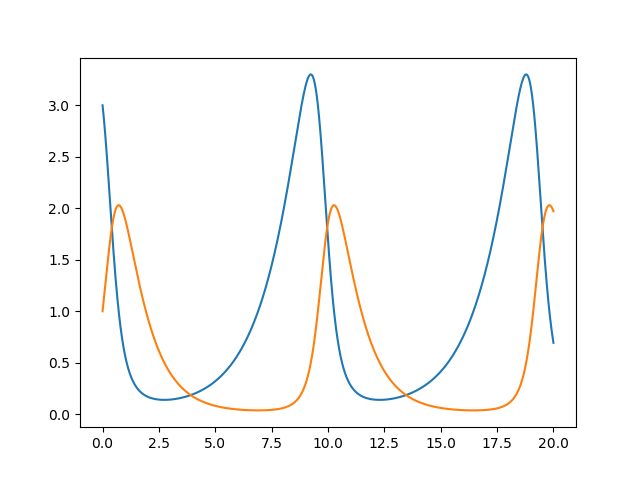
\includegraphics[width=.48\textwidth]{fig/lotkavolterra}
  \captionof{figure}{Plot of a solution to the Lotka-Volterra equation with
  parameters $\alpha = \frac 23$, $\beta  = \frac 43$, $\delta = \gamma = 1$
  and initial values $u(0) = 3$, $v(0) = 1$. Solved with a Runge-Kutta
  method of order five and step size $h = 10^{-5}$ \label{fig:lotkavolterra}}
  \end{center}
  Lotka and Volterra became interested in this system as they had
  found that the amount of predatory fish caught had increased
  during World War I. During the war years there was a strong
  decrease of fishing effort. In conclusion, they thought, there had
  to be more prey fish.
  
  A (far too rarely) applied consequence is that in order to diminish
  the amount of e.g. foxes one should hunt rabbits as foxes feed
  on rabbits.
\end{remark}

\begin{example}[Graviational two-body systems]
  According to Newton's law of universal gravitation, two bodies of
  masses $m_1$ and $m_2$ attract each other with a force
  \begin{gather*}
    \vec F_1 = G \frac{m_1m_2}{r^3} \vec r_1,
  \end{gather*}
  where $\vec F_1$ is the force vector acting on $m_1$ and $\vec r_1$
  is the vector pointing from $m_1$ to $m_2$ and $r = \lvert\vec r_1\rvert = \lvert\vec r_2\rvert$.

  Newton's second law of motion on the other hand relates forces and
  acceleration:
  \begin{gather*}
    \vec F = m \vec x'',
  \end{gather*}
  where $\vec x$ is the position of a body in space.

  Combining these, we obtain equations for the positions of the two bodies:
  \begin{gather*}
    \vec x''_i = G \frac{m_{3-i}}{r^3} (\vec x_i - \vec x_{3-i}), \qquad i=1,2.
  \end{gather*}
  This is a system of 6 independent variables. Nevertheless, it can be
  reduced to three by using that the center of mass moves
  inertially. Then, the distance vector is the only variable to be
  computed for:
  \begin{gather*}
    \vec r'' = - G \frac{m}{r^3} \vec r.
  \end{gather*}
  Intuitively, that we need an initial position and an initial
  velocity for the two bodies. Later on, we will see that this can
  actually be justified mathematically.
\end{example}

\begin{example}[Celestial mechanics]
  Now we extend the two-body system to a many-body system. Again, we
  subtract the center of mass, such that we obtain $n$ sets of 3
  equations for an $n+1$-body system. Since forces simply add up, this
  system becomes
  \begin{gather}
    \label{eq:celestial}
    \vec x_i = -G \sum_{j\neq i} \frac{m_j}{r_{ij}^3} \vec r_{ij}.
  \end{gather}
  Here, $\vec r_{ij} = \vec r_j - \vec r_i$ and $r_{ij} = \lvert \vec r_{ij}\rvert$.
  Initial data for the solar system can be obtained from
  \begin{center}
    \texttt{https://ssd.jpl.nasa.gov/?horizons}
  \end{center}
\end{example}

%%% Local Variables: 
%%% mode: latex
%%% TeX-master: "notes"
%%% End: 

%%%%%%%%%%%%%%%%%%%%%%%%%%%%%%%%%%%%%%%%%%%%%%%%%%%%%%%%%%%%%%%%%%%%%%
%%%%%%%%%%%%%%%%%%%%%%%%%%%%%%%%%%%%%%%%%%%%%%%%%%%%%%%%%%%%%%%%%%%%%%
\section{Introduction to initial value problems}
%%%%%%%%%%%%%%%%%%%%%%%%%%%%%%%%%%%%%%%%%%%%%%%%%%%%%%%%%%%%%%%%%%%%%%
%%%%%%%%%%%%%%%%%%%%%%%%%%%%%%%%%%%%%%%%%%%%%%%%%%%%%%%%%%%%%%%%%%%%%%


\begin{Definition*}{ode}{Ordinary differential equations}
  \defindex{differential equation!ordinary|see{ordinary differential equation}} \index{ODE|see{ordinary
      differential equation}} An \define{ordinary differential
    equation} (ODE) is an equation for a function $u(t)$, defined on
  an interval $I \subset \R$ and with values in the real or complex
  numbers or in the space $\R^d$ ($\C^d$), of the form
  \begin{gather}
    F\bigl(t, u(t), u'(t), u''(t), \dots, u^{(n)}(t)\bigr) = 0.
  \end{gather}
  Here $F(\ldots)$ denotes an arbitrary function of its arguments.
  The \textbf{order}\defindex{order!of a differential equation} $n$ of
  a differential equation is the highest derivative which occurs.  If
  the dimension $d$ of the value range of $u$ is higher than one, we
  talk about systems of differential equations.
\end{Definition*}

\begin{remark}
  A differential equation, which is not ordinary, is called partial.
  These are equations or systems of equations, which involve partial
  derivatives with respect to several independent variables.  While
  the functions in an ordinary differential equation may be dependent
  on additional parameters, derivatives are only taken with respect to
  one variable, typically, but not exclusively, this variable is
  time. Due to the fact that this manuscript just deals with ordinary
  differential equations, the adjective will be omitted in the
  following.
\end{remark}

\begin{Definition}{explicit-ode}{Explicit differential equation}
  \defindex{ordinary differential equation!explicit} An \define{explicit
    differential equation} of first order is a equation of the form
  \begin{align}
    \label{eq:awa:ode}
    u'(t) &= f(t,u(t))\\
    \text{or shorter:}\qquad u'&=f(t,u). \notag
  \end{align}
  A differential equation of order $n$ is called explicit, if it is of
  the form
  \begin{gather*}
    u^{(n)}(t) = F\left(t, u(t), u'(t), \ldots, u^{(n-1)}(t)\right)
  \end{gather*}
\end{Definition}
\begin{Lemma}{first-order}
  Every differential equation of higher order can be written as a
  system of first-order differential equations. If the equation is
  explicit, then the system is explicit.
\end{Lemma}

\begin{proof}
  By the introduction of additional variables $u_0(t) = u(t)$, $u_1(t)
  = u'(t)$ to $u_{n-1}(t) = u^{(n-1)}(t)$, each differential equation of
  order $n$ can be transformed into a system of $n$ differential equations
  of first order. This system has the form
  \begin{gather}
    \label{eq:awa:13}
    \begin{pmatrix}
      u_0'(t) - u_1(t) \\
      u_1'(t) - u_2(t) \\
      \vdots\\
      u_{n-2}'(t) - u_{n-1}(t) \\
      F\bigl(t, u_0(t),u_1(t),\dots,u_{n-1}(t), u_{n-1}'(t)\bigr)
    \end{pmatrix}
    =
    \begin{pmatrix}
      0\\0\\\vdots\\0\\0
    \end{pmatrix}.
  \end{gather}
  In the case of an explicit equation, the system has the form
  \begin{gather}
    \label{eq:awa:13a}
    \begin{pmatrix}
      u_0'(t) \\
      u_1'(t) \\
      \vdots\\
      u_{n-2}'(t) \\
      u_{n-1}'
    \end{pmatrix}
    =
    \begin{pmatrix}
      u_1(t)\\u_2(t)\\\vdots\\u_{n-1}(t)\\F\bigl(t, u_0(t),u_1(t),\dots,u_{n-1}(t)\bigr)
    \end{pmatrix}.
  \end{gather}
\end{proof}

\begin{example}
  \label{ex:awa:sine-1}
  The differential equation
  \begin{gather}
    \label{eq:awa:17}
    u'' + \omega^2 u = f(t)
  \end{gather}
  can be transformed into the system
  \begin{gather}
    \label{eq:awa:18}
    \begin{split}
      u_1' - u_2 &= 0, \\
      u_2' + \omega^2 u_1 &= f(t).
    \end{split}
  \end{gather}
  The transformation is not uniquely determined. In this example, a
  more symmetric system can be obtained:
  \begin{gather}
    \label{eq:awa:18a}
    \begin{split}
      u_1' - \omega u_2 &= 0, \\
      u_2' + \omega u_1 &= f(t).
    \end{split}
  \end{gather}
\end{example}

\begin{Definition}{autonomization}
  A differential equation of the form~\eqref{eq:awa:ode} is called
  \textbf{autonomous}, \defindex{autonomous differential equation} if
  the right hand side $f$ is not explicitly dependent on $t$, i.e.
  \begin{gather}
    u'=F(u).
  \end{gather}

  Each differential equation can be transformed into an autonomous
  differential equation.  This is called
  \textbf{autonomization}. \defindex{autonomization}
  \begin{equation*}
    U = \begin{pmatrix} u \\ t \end{pmatrix},
    \qquad
    F(U) = \begin{pmatrix} f(t,u) \\ 1 \end{pmatrix},
    \qquad
    U' = F(U)
  \end{equation*}

  A method which provides the same solution for the autonomous
  differential equation as for the original IVP, is called
  \textbf{invariant under autonomization}.
\end{Definition}


Differential equations usually provide sets of solutions from which we
have to choose a solution. An important selection criteria is setting
an initial value which leads to a well-posed problem (see below).

\begin{Definition}{IVP}
  \index{IVP|see{initial value problem}} Given a point
  $(t_0,u_0)\in \R \times \R^d$.  Furthermore, let the function
  $f(t,u)$ with values in $\R^d$ be defined in a neighborhood
  $I\times U \subset \R\times \R^d$ of the initial value.  Then an
  \define{initial value problem} (IVP) is defined as follows: find a
  function $u(t)$, such that
  \begin{subequations}
    \label{eq:awa}
    \begin{align}
      \label{eq:awa:2}
      u'(t)&=f\bigl(t,u(t)\bigr)
      \\
      \label{eq:awa:3}
      u(t_0)&=u_0
  \end{align}
  \end{subequations}
\end{Definition}
\begin{Definition}{local-solution}
    \label{def:awa:local solution}
  \defindex{solution!local} We call a continuously differentiable
  function $u(t)$ with $u(t_0) = 0$ a \define{local solution} of the
  IVP~\eqref{eq:awa}, if there exists a neighborhood $J$ of the point
  in time $t_0$ in which $u$ and $f(t,u(t))$ are defined and if the
  equation~\eqref{eq:awa:2} holds for all $t\in J$.
\end{Definition}

\begin{remark}
  We introduced the IVP deliberately in a ``local'' form because the
  local solution term is the most useful one for our purpose. Due to
  the fact that the neighborhood $J$ in the definition above can be
  arbitrarily small, we will have to deal with the extension to larger
  intervals below.
\end{remark}

\begin{remark}
  Through the substitution of $t\mapsto \tau$ with $\tau = t-t_0$ it
  is possible to transform every IVP at the point $t_0$ to a IVP in
  point $0$. We will make use of this fact and soon always assume
  $t_0 = 0$.
\end{remark}

\begin{Lemma}{volterra}
  Under the assumption that the right hand side $f$ is continuous in
  both arguments, the function $u(t)$ is a solution of the initial
  value problem~\eqref{eq:awa} if and only if it is a solution of the
  \define{Volterra integral equation} (VIE) \index{VIE!see{Volterra
      integral equation}}
  \begin{gather}
    \label{eq:volterra}
    u(t) = u_0 + \int_{t_0}^t f\bigl(s,u(s)\bigr)\ds.
  \end{gather}
  The formulation as integral equation allows on the other hand a more
  general solution term, because the problem is already well-posed for
  functions $f(t,u)$, which are just integrable with respect to $t$.
  In that case the solution $u$ would be just absolutely continuous
  and not continuously differentiable.
\end{Lemma}

%%% Local Variables: 
%%% mode: latex
%%% TeX-master: "../notes"
%%% End: 


\begin{remark}
  Both the theoretical analysis of the IVP and the numerical methods
  (with exception of the BDF methods) in this lecture notes, solve
  actually never the IVP~\eqref{eq:awa} but always the associated
  integral equation ~\eqref{eq:volterra}.
\end{remark}

\begin{Theorem*}{peano}{Peano's existence theorem}
  \defindex{Peano's theorem}
  \label{satz:peano}
  Let the function $f(t,u)$ be continuous on the closed set
  \begin{gather*}
    \overline D =\bigl\{
    (t,u) \in \R\times\R^d \;\big|
    \;|t-t_0| \le \alpha,\;
    |u-u_0|\le\beta
    \bigr\},
  \end{gather*}
  where $\alpha,\beta>0$. Then there exists a solution
    $u(t) \in C^1(I)$
  on the interval
    $I=[t_0-T,t_0+T]$
  with
  \begin{gather*}
    T=\min\left(\alpha ,\frac{\beta}{M}\right),\;
    M=\max_{(t,u)\in \overline D} \ |f(t,u)|.
  \end{gather*}
\end{Theorem*}


The proof of this theorem is of little consequence for the remainder
of these notes.  For its verification, we refer to textbooks on the
theory of ordinary differential equations.

\begin{remark}
  The Peano existence theorem does not make any statements about the
  uniqueness of a solution and also just guarantees local existence.
  The second limitation is addressed by the following theorem. The
  first will be postponed to section~\ref{sec:awa:well-posedness}.
\end{remark}

\begin{Theorem*}{peano-continuation}{Peano's continuation theorem}
  Let the assumptions of Theorem~\ref{satz:peano} hold. Then, the
  solution can be extended to an interval $I_m = [t_-, t_+]$ such that
  the points $\bigl(t_-,u(t_-)\bigr)$ and $\bigl(t_+,u(t_+)\bigr)$ are
  on the boundary of $\overline D$. Neither the values of $t$, nor of
  $u(t)$ need to be bounded as long as $f$ remains bounded.
\end{Theorem*}

\begin{example}
  The IVP
  \begin{gather*}
    u' = 2 \sqrt{\lvert u \rvert}, \qquad u(0) = 0,
  \end{gather*}
  has solutions $u(t) = t^2$ and $u(t) = 0$.
\end{example}

\begin{example}
  The functions $1/(t-t_0)$ are solutions to the IVP
  \begin{gather*}
    u'=-u^2, \qquad u(t_0) = 1.
  \end{gather*}
\end{example}

%%%%%%%%%%%%%%%%%%%%%%%%%%%%%%%%%%%%%%%%%%%%%%%%%%%%%%%%%%%%%%%%%%%%%%
%%%%%%%%%%%%%%%%%%%%%%%%%%%%%%%%%%%%%%%%%%%%%%%%%%%%%%%%%%%%%%%%%%%%%%
\section{Linear differential equations
  and Grönwall's inequality}
%%%%%%%%%%%%%%%%%%%%%%%%%%%%%%%%%%%%%%%%%%%%%%%%%%%%%%%%%%%%%%%%%%%%%%
%%%%%%%%%%%%%%%%%%%%%%%%%%%%%%%%%%%%%%%%%%%%%%%%%%%%%%%%%%%%%%%%%%%%%%

\begin{intro}
  The examination of linear differential equation turns out to be
  particularly simple. On the other hand, results obtained here will
  provide us with important statements for general non-linear
  IVP. Therefore we pay particular attention to the linear case.
\end{intro}

\begin{Definition}{linear-ode}
    \defindex{ordinary differential equation!linear} An IVP according to
  definition ~\ref{Definition:IVP} is called \textbf{linear} \defindex{linear
    differential equation} if the right hand side $f$ is an affine
  function of $u$. Thus, we can write it in the form
  \begin{subequations}    
    \label{eq:awa:4}
    \begin{xalignat}{2}
      \label{eq:awa:5}
      u'(t) &= A(t)u(t) + b(t)
      & \forall t &\in \R \\
      \label{eq:awa:6}
      u(t_0) &= u_0
    \end{xalignat}
  \end{subequations}
  with a continuous matrix function $A:\R\to \C^{d \times d}$. If in
  addition $b(t) \equiv 0$, we call it \define{homogeneous}.
\end{Definition}
\begin{Definition}{integrating factor}
    Let be the matrix function $A:I\to \C^{d\times d}$ continuous.  Then
  the function defined by
  \begin{gather}
    \label{eq:awa:7}
    M(t) = \exp\left(-\int_{t_0}^t A(s) \ds\right)
  \end{gather}
  is called \define{integrating factor} of the
  equation~\eqref{eq:awa:5}.
\end{Definition}

\begin{corollary}
  The integrating factor $M(t)$ has the properties
  \begin{align}
    \label{eq:awa:14}
    M(t_0) &= \identity\\
    \label{eq:awa:15}
    M'(t) &= -M(t)A(t).
  \end{align}
\end{corollary}

\begin{Lemma}{linear-representation}
  % Voraussetzungen an A und b
  A solution of the IVP~\eqref{eq:awa:4} is given through the 
  representation
  \begin{gather}
    \label{eq:awa:8}
    u(t) =  M(t)^{-1}\left(u_0 + \int_{t_0}^t M(s) b(s) \ds\right)
  \end{gather}
  with the integrating factor $M(t)$ of the equation~\eqref{eq:awa:7}.
  This solution exists for all $t\in \R$.
\end{Lemma}


%%% Local Variables:
%%% mode: latex
%%% TeX-master: "../notes"
%%% End:


\begin{proof}
  We consider the auxiliary function $w(t) = M(t) u(t)$ with the
  integrating factor $M(t)$ of the equation~\eqref{eq:awa:7}. Using the
  chain rule, there holds
  \begin{gather}
    \label{eq:awa:19}
    w'(t) =  M(t) u'(t) + M'(t) u(t)
    =  M(t) u'(t) - M(t)A(t)u(t).
  \end{gather}
  Comparing this to the differential equation~\eqref{eq:awa:5}, we see
  that $w$ solves
  \begin{gather*}
    w'(t) = M(t) b(t).
  \end{gather*}
	This can be integrated directly to obtain	
  \begin{gather*}
    w(t) = u_0 + \int_{t_0}^t M(t) b(t),
  \end{gather*}
  where we use that $w(t_0) = u_0$.  According to
  lemma~\ref{Lemma:appendix:exp-1}, about the \putindex{matrix
    exponential}, $M(t)$ is invertible for all $t$.  With the
  definition of $w(t)$ we are therefore able to solve for $u(t)$,
  which results in the equation~\eqref{eq:awa:8}. The global
  solvability follows from the fact that the solution is defined for
  arbitrary $t\in \R$.
\end{proof}

\begin{example}
  \label{ex:awa:sine-2}
  The equation in example~\ref{ex:awa:sine-1} is linear and can be
  written in the form of~\eqref{eq:awa:4} with
  \begin{align*}
    A(t) = A &=
    \begin{pmatrix}
      0 & \omega \\ -\omega & 0
    \end{pmatrix}
    \\
    b(t) &= f(t).
  \end{align*}
  Let now $f(t) \equiv 0$. The Jordan canonical form of $A$ is
  \begin{gather*}
    A = C^{-1}
    \begin{pmatrix}
      \omega i \\ & -\omega i
    \end{pmatrix}
    C
  \end{gather*}
  with a suitable transformation matrix $C$. The integrating factor is
  \begin{gather*}
    M(t) = e^{At} = C^{-1}
    \begin{pmatrix}
      e^{\omega i} \\ & e^{-\omega i}
    \end{pmatrix} C
    =
    \begin{pmatrix}
      \cos \omega t & \sin \omega t \\
      -\sin \omega t & \cos \omega t
    \end{pmatrix}.
  \end{gather*}
  Thus, given an initial value $(u_0, v_0)^T$, the solution is
  \begin{gather*}
    u(t) =  \begin{pmatrix}
      \cos \omega t & \sin \omega t \\
      -\sin \omega t & \cos \omega t
    \end{pmatrix}
    \begin{pmatrix}
      u_0\\v_0
    \end{pmatrix}.
  \end{gather*}
  The missing details in this argument and the case for an
  inhomogenety $f(t) = \cos \alpha t$ are left as an exercise.
\end{example}

\begin{remark}
  If the function $b(t)$ in~\eqref{eq:awa:5} is only integrable, the
  function $u(t)$ defined in~\eqref{eq:awa:8} is absolutely continuous
  and thus differentiable almost everywhere. The chain
  rule~\eqref{eq:awa:19} is applicable in all points of
  differentiability and $w(t)$ solves the Volterra integral equation
  corresponding to~\eqref{eq:awa:4}. Thus, the representation
  formula~\eqref{eq:awa:8} holds generally for solutions of linear
  Volterra integral equations.
\end{remark}

%%%%%%%%%%%%%%%%%%%%%%%%%%%%%%%%%%%%%%%%%%%%%%%%%%%%%%%%%%%%%%%%%%%%%%
\begin{Lemma*}{gronwall}{Grönwall}
  Let be $w(t)$, $a(t)$ and $b(t)$ be nonnegative, integrable
  functions, such that $a(t)w(t)$ is integrable. Furthermore, let
  $b(t)$ be monotonically nondecreasing and let $w(t)$ satisfy the
  integral inequality
  \begin{gather}
    \label{eq:awa:10}
    w(t) \le b(t) + \int_{t_0}^t a(s)w(s)\ds,\qquad t\ge t_.
  \end{gather}
  Then, for almost all $t \ge t_0$ there holds:
  \begin{gather}
    \label{eq:awa:11}
    w(t) \le b(t) \exp\left( \int_{t_0}^t  a(s) \ds\right).
  \end{gather}
\end{Lemma*}

%%% Local Variables:
%%% mode: latex
%%% TeX-master: "../notes"
%%% End:

\begin{proof}
  Using the integrating factor
  \begin{gather*}
    m(t) = \exp\left(-\int_{t_0}^t a(s) \ds\right),
    \quad
    \frac1{m(t)} = \exp\left(\int_{t_0}^t a(s) \ds\right),
  \end{gather*}
  we introduce the auxiliary function
  \begin{gather*}
    v(t) = m(t) % \exp\left(-\int_{t_0}^t a(s) \ds\right)
    \int_{t_0}^t a(s)w(s)\ds,
  \end{gather*}
  This function is absolutely continuous and almost everywhere
  \begin{gather*}
    v'(t) = m(t) a(t) %\exp\left(-\int_{t_0}^t a(s) \ds\right)
    \left[
      w(t) - \int_{t_0}^t a(s) w(s) \ds
    \right].
  \end{gather*}
  By assumption~\eqref{eq:awa:10}, the bracket on the right is bounded
  by $b(t)$. Thus,
  \begin{gather*}
    v'(t) \le m(t) a(t) b(t) %\exp\left(-\int_{t_0}^t a(s) \ds\right),
  \end{gather*}
  and since $v(t_0) = 0$ by its definition,
  \begin{gather*}
    v(t) \le \int_{t_0}^t m(s) a(s) b(s) % \exp\left(-\int_{t_0}^s a(r)
    \ds.
  \end{gather*}
  From the definition of $v(t)$, we obtain
  \begin{gather*}
    \int_{t_0}^t a(s)w(s)\ds = \frac1{m(t)} % \exp\left(\int_{t_0}^t a(s) \ds\right)
    v(t)
    \le \frac1{m(t)} \int_{t_0}^t m(s)a(s)b(s) \ds
    % \exp\left( %\int_{t_0}^t a(r) \dr
    %   - \int_{t_0}^s a(r) \dr\right)\ds
  \end{gather*}
  Finally, since $b(t)$ is nondecreasing we obtain almost everywhere
  \begin{align*}
    \int_{t_0}^t a(s)w(s)\ds
    &\le  \frac{b(t)}{m(t)} \int_{t_0}^t a(s)
    \exp\left(-\int_{t_0}^s a(r) \dr\right)\ds
    \\
    &= \frac{b(t)}{m(t)} \left[-
    \exp\left(-\int_{t_0}^s a(r) \dr\right)
      \right]_{t_0}^t
    \\
    &= \frac{b(t)}{m(t)} \bigl(m(t_0)-m(t)\bigr)
      = \frac{b(t)}{m(t)} - b(t)
  \end{align*}
  Now, entering into the integral inequality~\eqref{eq:awa:10}, we
  obtain
  \begin{gather*}
    w(t) \le b(t) + \int_{t_0}^t a(s)w(s)\ds = \frac{b(t)}{m(t)},
  \end{gather*}
  which proves the lemma.
\end{proof}

%%%%%%%%%%%%%%%%%%%%%%%%%%%%%%%%%%%%%%%%%%%%%%%%%%%%%%%%%%%%%%%%%%%%%%

\begin{remark}
	On the form of the requirements~\eqref{eq:awa:10} as well as the
  estimation~\eqref{eq:awa:11}, we can see that Grönwall's
  inequality is basically based on the construction of a majorant for 
	$w(t)$, which satisfies a linear IVP.
\end{remark}

%%%%%%%%%%%%%%%%%%%%%%%%%%%%%%%%%%%%%%%%%%%%%%%%%%%%%%%%%%%%%%%%%%%%%%
\begin{Corollary}{awa:unique-linear}
  Let the functions $u(t)$ and $v(t)$ be two solutions of the linear
  differential equation~\eqref{eq:awa:5}. If both functions
  coincide in a point $t_0$ then they are identical.
\end{Corollary}

\begin{proof}
	The difference $w(t) = v(t) - u(t)$ solves the integral equation
  \begin{gather*}
    w(t) = \int_{t_0}^t A(s) w(s) \ds.
  \end{gather*}
  Hence $|w(t)|$ satisfies the integral inequality
  \begin{gather*}
    |w(t)| \le \int_{t_0}^t |A(s)| |w(s)| \ds,
  \end{gather*}
	from which we conclude with Grönwall's inequality~\eqref{eq:awa:11} 
	for $b(t) = 0$, that $|w(t)|=0$ for all $t$ and therefore
  $u(t) = v(t)$.
\end{proof}

\begin{corollary}
  The representation formula~\eqref{eq:awa:8} in
  Lemma~\ref{Lemma:linear-representation} defines the unique solution to the
  IVP~\eqref{eq:awa:4}. In particular, solutions of linear IVP are
  always defined on the whole real axis.
\end{corollary}

\begin{example}
  Let $A \in \C^{d\times d}$ be diagonalizable with possibly repeated
  eigenvalues $\lambda_1,\dots,\lambda_d$ and corresponding
  eigenvectors $\psi^{(i)}$. Let $\Psi$ be the matrix of column
  vectors $\psi^{(i)}$. Then, the solution of the IVP
  \begin{gather*}
    \begin{split}
      u' &= A u,\\
      u(0) &= u_0,
    \end{split}
  \end{gather*}
  is given by the formula
  \begin{gather*}
    u(t) = e^{At} u_0 = \Psi \exp
    \begin{pmatrix}
      \lambda_1\\&\ddots\\&&\lambda_d
    \end{pmatrix}
    \Psi^{-1} u_0.
  \end{gather*}
  This is due to the fact, that $M(t) = e^{-At}$ and $e^{-\Psi A
    \psi^{-1}t} = \Psi e^{-At} \Psi^{-1}$.
\end{example}
%%%%%%%%%%%%%%%%%%%%%%%%%%%%%%%%%%%%%%%%%%%%%%%%%%%%%%%%%%%%%%%%%%%%%%

\begin{Lemma}{solution-space}
  \index{homogeneous}
  \index{ordinary differential equation!linear!homogeneous}
  The solutions of the homogeneous, linear differential equation
  \begin{gather}
    \label{eq:awa:9}
    u'(t) = A(t) u(t)
  \end{gather}
  with $u:\R\to\R^d$, define a vector space of dimension $d$. Let
  $\{\psi^{(i)}\}_{i=1,\dots,d}$ be a basis of $\R^d$. 
	Then the solutions $\phi^{(i)}(t)$ of the equation~\eqref{eq:awa:9} with 
  initial values $\phi^{(i)}(0) = \psi^{(i)}$ form a basis of the solution
  space. The vectors $\{\phi^{(i)}(t)\}$ are linear independent
  for all $t\in \R$.
\end{Lemma}


\begin{proof}
  At first we observe that for two solutions $u(t)$ and $v(t)$ of the
  equation~\eqref{eq:awa:9}, their sum and their scalar multiples are
  solutions too, due to linearity \index{linear} of the derivative
  and the right hand side.  Therefore the vector space structure is
  proven.
 
  Let now $\phi^{(i)}(t)$ be solutions of the IVP with linear
  independent initial values $\{\psi^{(i)}\}$.  As a consequence the
  functions are linear independent as well.

  Assume that $w(t)$ is a solution of the equation~\eqref{eq:awa:9},
  which cannot be written as a linear combination of $\psi^{(i)}$.
  Then $w(0)$ is not a linear combination of the vectors $\psi^{(i)}$:
  else let's say $w(0) = \sum \alpha_i \psi^{(i)}$, then
  $w(t) = \sum \alpha_i \phi^{(i)}(t)$ would be a linear combination
  because of uniqueness proven in
  corollary~\ref{Corollary:awa:unique-linear}.  Since $\{\psi^{(i)}\}$
  according to the assumtions is a basis of $\R^d$, such a $w(0)$
  cannot exist.  Hence it is shown that $\phi^{(i)}(t)$ is a basis of
  the solution space of dimension $d$.
  
  It remains to show that the $\phi^{(i)}(t)$ are linearly independent
  for all $t\in \R$. To this end, assume that the set $\phi^{(i)}(t)$
  is linearly dependent for a value $t_1$.  Then the following holds
  true without loss of generality
  \begin{gather*}
    \phi^{(d)}(t_1) = \sum_{i=1}^{d-1}\alpha_i\phi^{(i)}(t_1) =: w(t).
  \end{gather*}
  Again according to corollary~\ref{Corollary:awa:unique-linear} we
  have $\phi^{(d)} \equiv w$, moreover $\phi^{(d)}(0) = w(0)$ which
  again is a contradiction to the assumption $\psi^{(d)}$ is a linear
  combination of the other initial values.
\end{proof}

%%%%%%%%%%%%%%%%%%%%%%%%%%%%%%%%%%%%%%%%%%%%%%%%%%%%%%%%%%%%%%%%%%%%%%

\begin{Definition}{fundamental-system}
  A basis $\{\phi^{(1)},\dots,\phi^{(d)}\}$ of the solution space of
  the linear differential equation~\eqref{eq:awa:9}, in particular the
  basis with initial values $\phi^{(i)}(0) = e_i$, is called
  \define{fundamental system} of solutions.  The
  matrix function
  \begin{gather}
    \label{eq:awa:12}
    \fundam(t) =
    \begin{pmatrix}
      \phi^{(1)}(t)\dots\phi^{(d)}(t)
    \end{pmatrix}
  \end{gather}
  with column vectors $\phi^{(i)}(t)$ is called
  \define{fundamental matrix}.
\end{Definition}



\begin{Corollary}{fundamental-regular}
  The fundamental matrix is regular for all $t\in \R$ and solves the
  IVP
  \begin{align*}
    \fundam'(t) &= A(t)\fundam(t)\\
    \fundam (0) &= \identity.
  \end{align*}
\end{Corollary}

\begin{proof}
  The initial value is part of the definition. On the other hand,
  splitting the the matrix valued IVP into its column vectors, we
  obtain the original IVP defining the solution space. Regularity
  follows from linear independence of solutions for any $t$.
\end{proof}

%%%%%%%%%%%%%%%%%%%%%%%%%%%%%%%%%%%%%%%%%%%%%%%%%%%%%%%%%%%%%%%%%%%%%%
%%%%%%%%%%%%%%%%%%%%%%%%%%%%%%%%%%%%%%%%%%%%%%%%%%%%%%%%%%%%%%%%%%%%%%
\section{Well-posedness of the IVP}
%%%%%%%%%%%%%%%%%%%%%%%%%%%%%%%%%%%%%%%%%%%%%%%%%%%%%%%%%%%%%%%%%%%%%%
%%%%%%%%%%%%%%%%%%%%%%%%%%%%%%%%%%%%%%%%%%%%%%%%%%%%%%%%%%%%%%%%%%%%%%
\label{sec:awa:well-posedness}


\begin{Definition}{hadamard} 
  A mathematical problem is called \define{well-posed} if the
  following \textbf{Hadamard conditions} are satisfied:
  \index{Hadamard conditions}
  \begin{enumerate}
  \item A solution exists.
  \item The solution is unique.
  \item The solution is continuously dependent on the data.
  \end{enumerate}
  The third condition in this form is purely qualitative. Typically,
  in order to characterize problems with good approximation
  properties, we will require \putindex{Lipschitz continuity}, which
  has a more quantitative character.
\end{Definition}

%%% Local Variables:
%%% mode: latex
%%% TeX-master: "../notes"
%%% End:


\begin{example}
  The IVP
  \begin{gather*}
    u'= \sqrt[3]{u}, \qquad u(0) = 0,
  \end{gather*}
  has solutions of the form
  \begin{gather*}
    u(t) =
    \begin{cases}
      0 \\
      c \left(\tfrac23t\right)^{3/2}.
    \end{cases}
  \end{gather*}
  Thus, the solution is not unique and therefore, the IVP is not
  well-posed.
  Let now the initial value be nonzero, but slightly positive. Then, a small
  perturbation, which changes its sign, will have dramatic effect on
  the solution.
\end{example}

\begin{Definition}{Lipschitz-condition}
  The function $f(t,y)$ satisfies on its domain $D = I\times\Omega \subset
  \R \times \R^d$ an uniformly continuous \define{Lipschitz condition} if 
	it is Lipschitz continuous with regard to $y$, i.e., it exists a 
	positive constant $L$, such that
  \begin{gather}
    \label{eq:awa:1}
    \forall t\in I;\,x,y\in\Omega \;:\;
    \abs{f(t,x)-f(t,y)} \le L \abs{x-y}
  \end{gather}
  It satisfies a local Lipschitz condition if the same holds true for all 
  compact subsets of $D$.
\end{Definition}


\begin{example}
  Let $f(t,u)\in C^1(\R \times\R^d $ and let all partial derivatives
  with respect to components of $u$ be bounded by
  \begin{gather*}
    \max_{\substack{t\in \R\\u\in \R^d\\1\le i,j \le d}}
   \abs{
     \frac{\partial}{\partial u_i} f_j(t,u)
   } \le K.
  \end{gather*}
  Then, $f$ satisfies the Lipschitz condition~\eqref{eq:awa:1} with
  $L=K$. Indeed, by using Taylor expansion, we see that
  \begin{multline*}
    f_j(t, u) - f_j(t,v)
    = \int_0^1 \frac{d}{ds}f_j\bigl(t,u+s(v-u)\bigr)\ds\\
    = \int_0^1 \sum_{i=1}^d(u_i-v_i)\partial_if_j\bigl(t,u+s(v-u)\bigr)\ds.
  \end{multline*}
  It is an easy conclusion that
  \begin{gather*}
    \abs{f(t,u)-f(t,v)}
    \le K \abs{u-v}.
  \end{gather*}
\end{example}


\begin{Theorem*}{awa-stability}{Stability}
  Let $f(t,u)$ and $g(t,u)$ be two continuous functions on a
  cylinder $D = I \times \Omega$ where the interval $I$ contains
  $t_0$ and $\Omega$ is a convex set in $\R^d$.  Furthermore, let
  $f$ admit a Lipschitz condition with constant $L$ on $D$. Let $u$
  and $v$ be solutions to the IVP
  \begin{xalignat}{2}
    \label{eq:awa:20}
    u'&=f(t,u) \quad\forall t\in I,& u(t_0)&= u_0,\\
    \label{eq:awa:21}
    v'&=g(t,v) \quad\forall t\in I,& v(t_0)&= v_0.
  \end{xalignat}
  Then, there holds
  \begin{gather}
    \label{eq:awa:22}
    \abs{u(t)-v(t)} \le e^{L|t-t_0|}
    \left[ \abs{u_0-v_0}
      + \int_{t_0}^{t} \max_{x\in\Omega}
      \abs{f(s,x)-g(s,x)}\ds
    \right].
  \end{gather}
\end{Theorem*}

%%% Local Variables:
%%% mode: latex
%%% TeX-master: "../notes"
%%% End:


\begin{proof}
  Both $u(t)$ and $v(t)$ solve their respective Volterra integral
  equations. Taking the difference, we obtain
  \begin{align*}
    u(t)-v(t) &= u_0-v_0
           + \int_{t_0}^t \bigl[ f(s,u(s)) - g(s,v(s)) \bigr]\ds
    \\
         &= u_0-v_0
           + \int_{t_0}^t \bigl[ f(s,u(t)) - f(s,v(s)) \bigr]\ds
           + \int_{t_0}^t \bigl[ f(s,v(t)) - g(s,v(s)) \bigr]\ds.
  \end{align*}
  Thus, its norm admits the integral inequality
  \begin{align*}
    \abs{u(t)-v(t)}
    &\le \abs{u_0-v_0} + \int_{t_0}^t\abs{f(s,u(t)) - f(s,v(s))} \ds
    + \int_{t_0}^t \abs{f(s,v(t)) - g(s,v(s))} \ds
    \\
    &\le \underbrace{\abs{u_0-v_0}
      + \int_{t_0}^t \max_{x\in\Omega} \abs{f(s,x)-g(s,x)}\ds}_{b(t)}
      + \int_{t_0}^t L \abs{u(s)-v(s)} \ds.
  \end{align*}
  This inequality is in the form of the assumption in Grönwall's
  lemma, and its application yields the stability result.
\end{proof}


\begin{Theorem*}{picardlindelof}{Picard-Lindelöf}
  \defindex{Picard-Lindelöf theorem} 
  Let $f(t,y)$ be continuous on a cylinder
  \begin{gather*}
    D = \{ (t,y) \in \R \times
    \R^d | \ |t-t_0| \le a, |y-u_0| \le b \}.
  \end{gather*}
  Let $f$ be bounded such that there is a constant $M = \max_D
  \abs{f}$ and satisfy the Lipschitz condition~\eqref{eq:awa:1} with
  constant $L$ on $D$.  Then the IVP
  \begin{gather*}
    \begin{split}
      u' &= f(t,u) \\ u(t_0) &= u_0
    \end{split}
  \end{gather*}
  is uniquely solvable on the interval
  $I = [t_0-T,t_0+T]$ where
  $T = \min \{ a, \frac{b}{M} \}$.
\end{Theorem*}

%%% Local Variables:
%%% mode: latex
%%% TeX-master: "../notes"
%%% End:


\begin{proof}
  First, we assume for simplicity $t_0=0$ or we transform the problem
  accordingly. Abbreviate $I = [-T,T]$ and
  \begin{gather*}
    \Omega = \bigl\{x\in \R^d\big| \abs{x-u_0} \le b \bigr\}.
  \end{gather*}

  We introduce the operator $F(u)$ which is defined
  through the \putindex{Volterra integral
    equation}~\eqref{eq:volterra} as
  \begin{gather}
    \label{eq:awa:16}
   F(u)(t) = u_0 + \int\limits_{0}^t f(s,u(s)) \ds.
  \end{gather}
  Obviously $u$ is a solution of the Volterra integral
  equation~\eqref{eq:volterra} if and only if $u$ is a \putindex{fixed
    point} of $F$ i.e., $u=Fu$. We can obtain such a fixed-point by
  the iteration $u^{(k+1)} = F(u^{(k)})$ with some initial guess
  $u^{(0)}:I\to\Omega$. From the boundedness of $f$, we obtain for
  $t-t_0 \le T$
  \begin{align*}
    \abs{u^{(k+1)}(t)-u_0} = \abs{\int_{t_0}^t f(s,u^{(k)}(s))\ds} \le \int_{t_0}^t
    \abs{f(s,u^{(k)}(s))}\ds \le TM \le b.
  \end{align*}
  Thus, from $u^{(0)}:I\to\Omega$ follows $u^{(k)}:I\to\Omega$ for all
  $k$ and the iteration is well-defined.
  
  We now show that $F$ is a contraction under the assumtions of the
  theorem. We follow the technique
  in~\cite[\S117]{Heuser86} and choose on the space $\mathcal C(I)$,
  which is the space of the continuous functions on $I$, the norm
  \begin{gather*}
    \norm{u}_e := \underset{t \in I}{max} ~e^{-2 L t} |u(t)|.
  \end{gather*}
  
  With estimating the difference of operator $F$ applied to two functions:
  \begin{align*}
    |F(u)(t) - F(v)(t)|
    & = \left| u_0 - u_0 + \int\limits_{0}^t (f(s,u(s)) - f(s,v(s))) \ds \right| \\
    & \le \int\limits_{0}^t \left| f\bigl(s,u(s)\bigr) - f\bigl((s,v(s)\bigr) \right| \ds \\
    & \le \int\limits_{0}^t L |u(s) - v(s)| \underbrace{e^{-2 L s} e^{2 L s}}_{= 1} \ds \\
    & \le L \norm{u-v}_e \int\limits_{0}^t e^{2 L s} \ds \\
    & = L \norm{u-v}_e \frac{e^{2 L t} - 1}{2 L} \\
    & \le \frac12 e^{2 L t} \norm{u-v}_e.
  \end{align*}

  It follows   
  \begin{gather*}
    e^{-2 L t}|F(u)(t) - F(v)(t)| \le \frac12 \norm{u-v}_e,
  \end{gather*}
  for all $t$ and we observe:
  \begin{gather*}
    |F(u)(t) - F(v)(t)|_e \le \frac12 \norm{u-v}_e.
  \end{gather*}
  Thus, we have shown that $F$ is a contraction on the space of the
  continuous functions with the norm $\norm{.}_e$.  Therefore, we can apply
  the \putindex{Banach fixed-point theorem}, concluding that $F$ has
  exactly one fixed-point. This proves the theorem.
\end{proof}

\begin{remark}
  The norm $\norm{u}_e$ had been chosen with regard to Grönwall's
  inequality, which was not used in the proof explicitly.  It is
  equivalent to the norm $\norm{u}_\infty$ because $e^{-2 L t}$ is strictly
  positiv and bounded. On the other hand one could have performed the
  proof with some more calculations with respect to the ordinary
  Tchebychev distance (maximum norm) $\norm{u}_\infty$.
\end{remark}

\begin{remark}
  Currently our solution is restricted to $I = [t_0 - T, t_0 + T]$.
  Since $T$ is chosen in such a way in
  equation~\ref{Theorem:picardlindelof} that the graph of $u$ does not
  leave the domain, this extension always ends on the boundary of
  $D$. One can now extend the solution by solving the next IVP
  $\left\{\begin{array}{l}
            u' = f(t,u)\\
            u(t_1) = u_1\\
  \end{array}\right\}$
	on the interval $I_1$. This way one obtains a solution on
 $I \cup I_1 \cup I_2 \cup ...$.
\end{remark}

\begin{corollary}
  Let the function $f(t,u)$ admit the Lipschitz condition on $\R\times
  \C^d$. Then, the IVP has a unique solution on the whole real axis.
\end{corollary}

\begin{proof}
  The boundedness was used in order to guarantee that $u(t)\in \Omega$
  for any $t$. This is not necessary anymore, if $\Omega =
  \C^d$. Thus, the limitation of the interval $I$ becomes unnecessary
  as well. Finally, the fixed point argument does not depend on
  boundedness of the set.
\end{proof}
% \begin{theorem}[Differential stability]
%   In addition to the assumptions of the Picard-Lindelöf theorem, let
%   the gradient of $f$ with respect to its second argument, $\nabla_u
%   f(t,u)$ exist and be continuous in $D$. Then, the solution of the
%   IVP depends continuously on the initial value $u_0$ and the gradient
%   of the solution $u$ with respect to $u_0$ solves the IVP
%   \begin{gather}
%     \label{eq:awa:23}
%     \begin{split}
%     (\nabla_{u_0} u)' &= \nabla_u f(t,u) \nabla_{u_0} u,
%     \\
%     \nabla_{u_0} u(t_0) &= \mathbb I.
%     \end{split}
%   \end{gather}
% \end{theorem}

%%%%%%%%%%%%%%%%%%%%%%%%%%%%%%%%%%%%%%%%%%%%%%%%%%%%%%%%%%%%%%%%%%%%%%
%%%%%%%%%%%%%%%%%%%%%%%%%%%%%%%%%%%%%%%%%%%%%%%%%%%%%%%%%%%%%%%%%%%%%%
%\section{Examples}
%%%%%%%%%%%%%%%%%%%%%%%%%%%%%%%%%%%%%%%%%%%%%%%%%%%%%%%%%%%%%%%%%%%%%%
%%%%%%%%%%%%%%%%%%%%%%%%%%%%%%%%%%%%%%%%%%%%%%%%%%%%%%%%%%%%%%%%%%%%%%

% \begin{example}
% 	It exists a solution of the IVP
%     $\left\{\begin{array}{l}
%       u'=\sin(u)\\
%       u(0)=7\\
%     \end{array}\right\}$?

%   \begin{enumerate}
%     \item The IVP is autonomous.
%     \item $|\sin(u)| \le 1$
%     \item $\sin(u)$ satisfies the Lipschitz condition with $L=1$.
%     \item $D = \R \times \R$
%   \end{enumerate}

%   $\Rightarrow$ Due to the theorems of Peano~\eqref{satz:peano} and Picard-Lindelöf~\eqref{Theorem:picardlindelof} it follows:
%   $\exists! u : \R \to \R$
% \end{example}

% \begin{example}
%   $\left\{\begin{array}{l}
%     u'(t) = -u^2\\
%     u(-1) = 1\\
%   \end{array}\right\}$

%   \begin{enumerate}
%     \item $u^2$ is continuous in $\R$.
%     \item However we just have a local Lipschitz condition.
%   \end{enumerate}
%   \noindent $\Rightarrow$ $u(t) = \frac1t$ auf $(-\infty,0)$
% \end{example}

% \begin{example}
%   $\left\{\begin{array}{l}
%     u' = \lambda u\\
%     u(0) = u_0\\
%   \end{array}\right\}$

% 	\begin{enumerate}
%   \item $\lambda u$ is Lipschitz continuous on $\R$
% 	\end{enumerate}

%   \noindent $\Rightarrow e^{\lambda t} u_0$ is the unique solution in $\R$.
% \end{example}


%%% Local Variables: 
%%% mode: latex
%%% TeX-master: "main"
%%% End: 

\chapter{Explicit One-Step Methods and Convergence}

\section{Introduction}
\begin{example}[Euler's method]
  We begin this section with the method which serves as prototype for
  a whole class of schemes which solves an IVP or rather the Volterra
  integral equation numerically. Here, as always for problems with
  infinite dimensional solution spaces, numerical solution refers to
  finding an approximation by applying a discretization method, and
  studying the error of this method.
  
  Consider the following problem: given an IVP of the form~\eqref{eq:awa},
  calculate the value $u(T)$ at a later point in time $T$.
  
  To this end, we note first of all that for an IVP at the initial
  point $0$, not only the function value $u(0) = u_0$ is known,
  but also the derivative $u'(0) = f(0, u_0)$. Thus we are capable
  to replace the solution $u(t)$ in blue by a straight line $y(t)$ in
  red, which we can see on the left of Figure~\ref{fig:explicit:Euler}.
  \begin{figure}[tp]
    \centering
    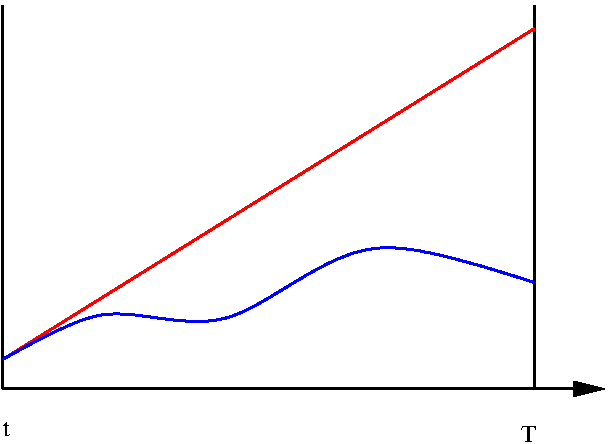
\includegraphics[width=.48\textwidth]{fig/euler1}
    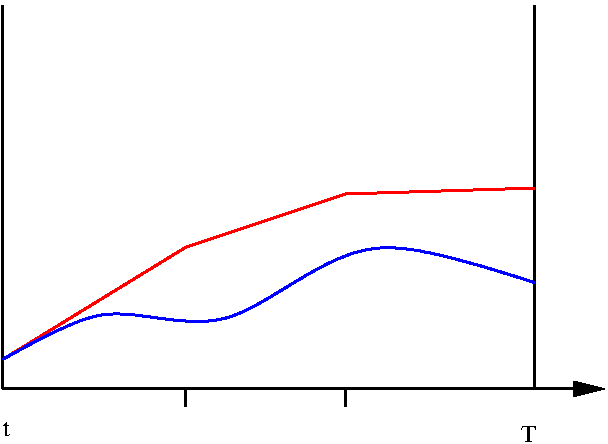
\includegraphics[width=.48\textwidth]{fig/euler2}
    \caption{Derivation of the Euler method. Left: replacement of the
			solution of the IVP by a line with slope and initial point given 
			by the IVP. Right: Euler method with three subintervals.}
    \label{fig:explicit:Euler}
  \end{figure}
  The figure suggests that in general the accuracy of this method may
  not be very good. The first improvement is that we do not draw the
  line through the whole interval from $0$ to $T$.  Instead, we
  insert intermediate points and apply the method to each subinterval,
  where we use the result of a previous interval as the initial point
  for the next subinterval.  As a result one obtains a
  chain of straight lines and the so-called \define{Euler method}.
\end{example}


\begin{Definition}{partitioning}
  On a time interval $I = [0,T]$, we define a partitioning in $n$
  subintervals, also known as \textbf{time steps}.\defindex{time step}
  Here we choose the following notation:
%  \begin{figure}[tp]
  \begin{center}
    \small
    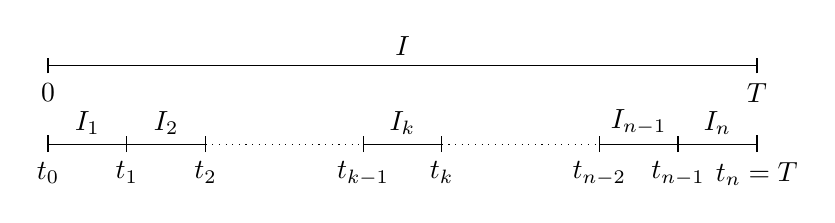
\begin{tikzpicture}
      \draw(0,1) -- node [anchor=south]{$I$} (9,1);
      \draw[thick](0,.9) node[anchor=north]{$0$} -- (0,1.1);
      \draw[thick](9,.9) node[anchor=north]{$T$} --(9,1.1);

      \draw(0,0)-- node [anchor=south]{$I_1$}(1,0);
      \draw(1,0)-- node [anchor=south]{$I_2$}(2,0);
      \draw(4,0)-- node [anchor=south]{$I_k$}(5,0);
      \draw(7,0)-- node [anchor=south]{$I_{n-1}$}(8,0);
      \draw(8,0)-- node [anchor=south]{$I_{n}$}(9,0);
      \draw[dotted](2,0)--(4,0);
      \draw[dotted](5,0)--(7,0);
      \draw[thick](0,-.1) node[anchor=north]{$t_0$} -- (0,.12);
      \draw(1,-.1) node[anchor=north]{$t_1$} --(1,.1);
      \draw(2,-.1) node[anchor=north]{$t_2$} --(2,.1);
      \draw(4,-.1) node[anchor=north]{$t_{k-1}$} --(4,.1);
      \draw(5,-.1) node[anchor=north]{$t_k$} --(5,.1);
      \draw(7,-.1) node[anchor=north]{$t_{n-2}$} --(7,.1);
      \draw(8,-.1) node[anchor=north]{$t_{n-1}$} --(8,.1);
      \draw[thick](9,-.1) node[anchor=north]{$t_n=T$} --(9,.12);
    \end{tikzpicture}
  \end{center}
%    \caption{Partition of the interval $I=[0,T]$ in subintervals $I_1,\dots,I_n$.}
%    \label{fig:explicit:schritte}
%  \end{figure}
  The time steps $I_k = [t_{k-1},t_{k}]$ have the step size
  $h_k = t_{k} - t_{k-1}$.  A partitioning in $n$ time steps implies
  $t_n = T$.  The term $k$-th time step is used for both the interval
  $I_k$ and for the point in time $t_k$, but it should always be clear
  through context which one is meant.

  Very often, we will consider evenly spaced time steps, in which case
  we denote the step size by $h$ and $h_k=h$ for all $k$.
\end{Definition}

%%% Local Variables:
%%% mode: latex
%%% TeX-master: "../notes"
%%% End:


\begin{definition}
  In the following chapters we will regularly compare the solution of
  an IVP with the results of discretization methods. Therefore, we
  introduce the following convention for notations and symbols.
  
  \defindex{solution!continuous}\defindex{solution!exact} The solution
  of the IVP is called the \textbf{exact} or \define{continuous
    solution}\defindex{exact solution}. The term ``continuous''
  indicates here the solution of the non-discretized problem. Its
  symbol is in general $u$ and we set as abbreviation
  \begin{gather*}
    u_k = u(t_k).
  \end{gather*}
  If $u$ is vector-valued we also use the alternative superscript
  $u^{(k)}$ and $u_i^{(k)}$ for a entry of the vector $u(t_k)$.

  \defindex{solution!discrete} In general we write the
  \define{discrete solution} with the
  symbol $y$. We write $y_k$ or $y^{(k)}$ for the value of the
  discrete solution at the point in time $t_k$. In contrast to the
  continuous solution, $y$ only defined at discrete time steps, unless
  for special methods discussed later.
\end{definition}

\begin{Definition*}{one-step}{Explicit one-step method}
  \defindex{One-step method!explicit} An \textbf{explicit one-step
    method} \defindex{Explicit one-step method} is a method which,
  given $u_0$ at $t_0 = 0$ computes a sequence of approximations
  $y_1\,\dots,y_n$ to the solution of an IVP in the time steps
  $t_1,\dots,t_n$ using an update formula of the form\footnote{The adjective
  `explicit' is here in contrast to `implicit'
  one-step methods, where the increment function depends 
	on $y_{k}$ and equation~\eqref{eq:explicit:8} must be solved
        for $y_{k}$.}
  \begin{gather}
    \label{eq:explicit:8}
    y_{k} = y_{k-1} + h_{k} \verfahren_{h_k}(t_{k-1},y_{k-1}).
  \end{gather}
  The function $\verfahren()_{h_k}$ is called \define{increment
    function}.  We will often omit the index $h_k$ on
  $\verfahren_{h_k}()$ because it is clear that the method is always
  applied to time intervals.

  The method is called \textbf{one-step method}
  because the value $y_{k}$ explicitly depends only of the values
  $y_{k-1}$ and $f(t_{k-1}, y_{k-1})$, not on previous values.
\end{Definition*}

%%% Local Variables:
%%% mode: latex
%%% TeX-master: "../notes"
%%% End:


\begin{remark}
  \label{remark:expl:first-step}
  For one-step methods every step is \emph{per definitionem} similar.
  Therefore, it is sufficient to consider the first step only.  Hence,
  we will define and analyze methods by stating the dependence of
  $y_1$ on $y_0$, which then can be transferred to the general step
  from $y_{n-1}$ to $y_{n}$. The general one-step method above then
  reduces to
  \begin{gather*}
    y_1 = y_0 + h \verfahren(t_0, y_0).
  \end{gather*}
  This implies that the values $y_k$ with $k\ge 2$ are computed
  through formula~\eqref{eq:explicit:8} with the respective $h_k$ and
  the same increment function.
\end{remark}

\begin{Example}{euler-linear-1}
  Given the IVP
  \begin{xalignat*}2
    u'  &= u,&
    u(0) &= 1,    
  \end{xalignat*}  
  the solution is $u(t) = e^t$. The Euler method reads
  \begin{gather*}
    y_1 = y_0 + h y_0.
  \end{gather*}
  The results for $h=1$ and $h=1/2$ are:
  \begin{center}
    \begin{tabular}{cc|ccc|ccc}
      \multicolumn{2}{c|}{exact}
      &\multicolumn{3}{c|}{$h=1$}
      &\multicolumn{3}{c}{$h=1/2$}\\\hline
      $t=0$ & 1           & $y_0$ & 1     && $y_0$ & 1 & \\
      $t=1$ & 2.71828     & $y_1$ & 2     & 0.718 & $y_2$ & 2.25  & 0.468\\
      $t=2$ & 7.38906     & $y_2$ & 4     & 3.389 & $y_4$ & 5.0625& 2.236\\\hline
      $t=k$ & $2.71828^k$ & $y_k$ & $2^k$ && $y_{2k}$ & $2.25^k$
    \end{tabular}    
  \end{center}
  We note that the error is growing in time. The approximation of the
  solution can be improved by shrinking $h$ from 1 to 1/2. The goal of
  error analysis will be establishing these dependencies.
\end{Example}

%%% Local Variables:
%%% mode: latex
%%% TeX-master: "../notes"
%%% End:


%%%%%%%%%%%%%%%%%%%%%%%%%%%%%%%%%%%%%%%%%%%%%%%%%%%%%%%%%%%%%%%%%%%%%%
%%%%%%%%%%%%%%%%%%%%%%%%%%%%%%%%%%%%%%%%%%%%%%%%%%%%%%%%%%%%%%%%%%%%%%
\section{Error analysis}
%%%%%%%%%%%%%%%%%%%%%%%%%%%%%%%%%%%%%%%%%%%%%%%%%%%%%%%%%%%%%%%%%%%%%%
%%%%%%%%%%%%%%%%%%%%%%%%%%%%%%%%%%%%%%%%%%%%%%%%%%%%%%%%%%%%%%%%%%%%%%

\begin{remark}
  In Figure~\ref{fig:explicit:Euler}, we observe that the error
  consists of two parts at a given time $t_{k+1}$. First, an error on
  the interval $I_k$ due to replacing the differential equation by the
  discrete method. Second, we have to add the error which results from
  the fact, that our initial value $y_k$ is already not exact due to
  previous errors. This situation is displayed in
  Figure~\ref{fig:forward-errors}. After one time step, a local error
  has appeared. In the second time step, we already start with an
  erroneous initial value. Therefore, we split the error into the
  local error and an accumulated error. The local error compares
  continuous and discrete solutions on a single interval with the same
  initial value. In the analysis, we will have the options of using
  the exact (right figure) or the approximated initial value (left figure).

  \begin{figure}[tp]
    \centering
    \includegraphics[width=.49\textwidth]{fig/forward-error.tikz}
    \includegraphics[width=.49\textwidth]{fig/backward-error.tikz}
    \caption{Local and accumulated errors. Exact solution in black,
      the Euler method in red. On the left, in blue the exact solution
      of an IVP on the second interval with initial value $y_1$. On
      the right, in purple the second step of the Euler method, but with
      exact initial value $u_1$.}
    \label{fig:forward-errors}
  \end{figure}
\end{remark}

\begin{Definition}{truncation-error}
  Let $u$ be a solution of the differential equation $u' = f(t,u)$
  on the interval $I_n = [t_{n-1}, t_{n}]$. Then, the \define{local
    error} of a discrete method $F$ is the difference between the
  solution $u_n$ of the differential equation at $t_n$ and the result
  of one time step~\eqref{eq:explicit:8} with this method with exact
  initial value:
  \begin{gather}
    \label{eq:explicit:6a}
    \eta_{n} = \eta_n(u) = u_{n} - \bigl[
    u_{n-1} + h_n \verfahren_{h_n}(t_{n-1}, u_{n-1})
    \bigr].
  \end{gather}
  The \define{truncation error} is the quotient of the local error and $h_n$:
  \begin{gather}
    \label{eq:explicit:6}
    \tau_{n} = \tau_n(u) = \frac{u_{n} - u_{n-1}}{h_n} - \verfahren_{h_n}(t_{n-1}, u_{n-1}).
  \end{gather}
  \defindex{order!of consistency}
  The one-step method $F_h(t,y)$ is \define{consistent} of \textbf{order} $p$ with
  the ODE, if there is a constant $c$ independent of $h$ such that for
  $h\to 0$:
  \begin{gather}
    \label{eq:explicit:3}
    \max\limits_n \abs{\tau_n} \le c h^p
  \end{gather}
\end{Definition}

%%% Local Variables:
%%% mode: latex
%%% TeX-master: "../notes"
%%% End:


\begin{example}[Euler method]
  To find out the order of consistency of the Euler method, we 
  consider the Taylor expansion of the solution at the point $t_{n-1}$:
  \begin{equation*}
    u(t_n) = u(t_{n-1}) + h_n u'(t_{n-1}) + \frac12 h_n^2 u''(\zeta)
  \end{equation*}
  
  As a result the truncation error reduces to:
  
  \begin{equation*}\begin{split}
    \tau_n & = \frac{u_n - u_{n-1}}{h_n} - F(h;t_{n-1},u(t_{n-1})) \\
    & = \frac{u_{n-1} + h_n f(t_{n-1},u_{n-1})
      + \frac12 h_n^2 u''(\zeta) - u_{n-1}}{h_n} - f(t_{n-1}; u_{n-1}) \\
    & = \frac12 h_n u''(\zeta)
  \end{split}\end{equation*}

% For $u''(\zeta)$ however there holds:
% \begin{equation*}
%   u''(\zeta) = \diffq[\zeta] f(\zeta,u(\zeta)) = \pdiffq[\zeta] f(\zeta,u(\zeta)) + \pdiffq[u] f(\zeta,u(\zeta)) \underbrace{u'(\zeta)}_{= f(\zeta,u(\zeta))}
% \end{equation*}

Under the assumption that $f \in C^1$ on a compact set around the graph
of $u$, this term is bounded, yielding.
\begin{gather*}
  | \tau_n | \le \frac{h_n}{2} \max_{\zeta\in I_n} \abs{u''(\zeta)}
  = \frac{h_n}{2} \max_{\zeta\in I_n} \bigl|\partial_x f(\zeta,
    u(\zeta)) + \partial_u  f(\zeta, u(\zeta)) f(\zeta, u(\zeta))\bigr|
\end{gather*}
Here, we enter the assumption that $f$ is sufficiently smooth to
conclude that the Euler method is consistent of order 1.
\end{example}

\begin{Lemma*}{gronwall-discrete}{Discrete Grönwall inequality}
  \index{Grönwall's inequality} Let $(w_n)$, $(a_n)$ and $(b_n)$ be
  non-negative sequences of real numbers. Let $b_n$ be monotonically
  nondecreasing. Then, if
  \begin{gather}
    \label{eq:gronwall-discrete:1}
    w_0 \le b_0
    \quad\text{and}\quad
    \forall n\ge 1 :\;
    w_n \le \sum\limits_{k=0}^{n-1} a_k w_k + b_n,
  \end{gather}
  there holds
  \begin{gather}
    \label{eq:explicit:5}
    w_n \le \exp \left(\sum\limits_{k=1}^{n-1} a_k\right) b_n.
  \end{gather}
\end{Lemma*}

%%% Local Variables:
%%% mode: latex
%%% TeX-master: "../notes"
%%% End:


\begin{proof}
  Define the functions $w(t)$, $a(t)$, and $b(t)$ such that for $k\ge
  1$ and $t\in [k-1,k)$ there holds
  \begin{gather*}
    w(t) = w(t_{k-1}),\quad
    a(t) = b(t_{k-1}),\quad
    b(t) = b(t_{k-1}).
  \end{gather*}
  These functions are bounded and piecewise continuous on any finite
  interval. Thus, they are integrable on $[0,n]$. Therefore, the
  continuous Grönwall inequality of Lemma~\ref{Lemma:gronwall} applies
  and proves the result.
\end{proof}

\begin{Theorem*}{stability-discrete}{Discrete stability}
  If $F(t,y)$ is Lipschitz continuous in $y$ for any $t=t_k$, $k<n$,
  with constant $L_h$, then the one-step method is \define{discretely
    stable}, i.~e. for arbitrary sequences $(y_n)$ and $(z_n)$, there
  holds: if $\eta_k(y)$ and $\eta_k(z)$ are both bounded independent
  of the sequences $(y_n)$ and $(z_n)$, then
  \begin{equation*}
    \abs{y_n - z_n}
    \le e^{L_h(t_n-t_0)} \left(
      \abs{y_0 - z_0}
      + \sum_{k=1}^n \abs{\eta_k(y) - \eta_k(z)}
    \right)
  \end{equation*}
\end{Theorem*}

%%% Local Variables:
%%% mode: latex
%%% TeX-master: "../notes"
%%% End:


\begin{proof}
  Subtracting the equations
  \begin{align*}
    \eta_k(y) &= y_k-y_{k-1} - \verfahren_{h_k}(t_{k-1},y_{k-1}),
    \\
    \eta_k(y) &= z_k-z_{k-1} - \verfahren_{h_k}(t_{k-1},z_{k-1}),
  \end{align*}
  we obtain
  \begin{multline*}
    y_k-z_k = y_{k-1} - z_{k-1} + \eta_k(y) - \eta_k(z)
    \\
    + h_k \bigl(
      F_{h_k}(t_{k-1},y_{k-1})-F_{h_k}(t_{k-1},z_{k-1})
    \bigr)
    .
  \end{multline*}
  Recursive application yields
  \begin{gather*}
    \abs{y_n-z_n} \le \abs{y_0-z_0}
    + \sum_{k=1}^n \abs{\eta_k(y)-\eta_k(z)}
    + \sum_{k=1}^n L_h h_{k} \abs{y_k-z_k}.
  \end{gather*}
  The estimate now follows from the discrete Grönwall inequality in
  Lemma~\ref{Lemma:gronwall-discrete}.
\end{proof}

\begin{corollary}
  Let the one-step method $\verfahren$ be run on a computer, yielding
  a sequence $(z_n)$, such that each time step is executed in finite
  precision arithmetic. Let $(y_n)$ be the mathematically correct
  solution of the one-step method. Then, the difference
  equation~\eqref{eq:explicit:8} is fulfilled only up to machine
  accuracy $\epsilon_m$:
  \begin{align*}
    y_0-z_0 &\approx \epsilon_m \\
    \abs{\eta_k(y) - \eta_k(z)} &= \abs{\eta_k(z)} \approx \epsilon_m \abs{z_k}.
  \end{align*}
  Then, the error between the true solution of the one-step method
  $(y_n)$ and the computed solution is bounded by
  \begin{gather*}
    \abs{y_n-z_n} \le e^{L_h(t_n-t_0)} n \epsilon_m \max_k\abs{z_k}.
  \end{gather*}
\end{corollary}

\begin{Theorem*}{convergence-one-step}{Convergence of one-step methods}
  Let the one-step method $F(.,.)$ be consistent of order $p$ and
  discretely stable, that is, $F(.,.)$ is Lipschitz continuous in its
  second argument. Let $f(t,u)\in C^{p}$. Furthermore, let be
  $y_0 = u_0$. Then the method converges with order $p$ and there
  holds for $h = \max h_n$
  \begin{equation}
    \label{eq:convergence-onestep:1}
    \abs{u_n - y_n} \le c e^{L_h(t_n-t_0)} h^p,
  \end{equation}
  where the constant $c$ is independent of $h$.
\end{Theorem*}

%%% Local Variables:
%%% mode: latex
%%% TeX-master: "../notes"
%%% End:


\begin{proof}
  Again we use the discrete stability theorem: with the definition of
  the order of the method, we obtain
  \begin{gather*}
    \abs{\eta_k(u)-\eta_k(y)} = \abs{\eta_k(u)} \le c h^{p+1},
  \end{gather*}
  where $c$ depends on the derivatives of $u$ (and thus of $f$), but
  not on $u_k-y_k$. Thus, we obtain
  \begin{gather*}
    \abs{u_n-y_n} \le e^{L_h(t_n-t_0)}\sum_{k=1}^n h_k^{p+1}
    \le e^{L_h(t_n-t_0)} h^p.
  \end{gather*}
\end{proof}

\begin{corollary}
  The Euler method converges of first order.
\end{corollary}

%%%%%%%%%%%%%%%%%%%%%%%%%%%%%%%%%%%%%%%%%%%%%%%%%%%%%%%%%%%%%%%%%%%%%%
%%%%%%%%%%%%%%%%%%%%%%%%%%%%%%%%%%%%%%%%%%%%%%%%%%%%%%%%%%%%%%%%%%%%%%
\section{Runge-Kutta methods}
%%%%%%%%%%%%%%%%%%%%%%%%%%%%%%%%%%%%%%%%%%%%%%%%%%%%%%%%%%%%%%%%%%%%%%
%%%%%%%%%%%%%%%%%%%%%%%%%%%%%%%%%%%%%%%%%%%%%%%%%%%%%%%%%%%%%%%%%%%%%%

\begin{intro}
  We are searching for methods which approximate the solution to an
  IVP numerically.  In fact we are not solving the IVP, but the Volterra
  integral equation~\eqref{eq:volterra}.  Hence we can consider
  solving differential equations as a quadrature problem; with the
  difficulty that the function, which we integrate, is not known. This
  consideration leads to a class of methods for IVP, the
  Runge-Kutta methods.
\end{intro}

\begin{Definition}{erk}
  \defindex{Runge-Kutta method!explicit (ERK)}
  \index{ERK|see{Runge-Kutta method}} 
  An \textbf{explicit Runge-Kutta method (ERK)} is a
  one-step method with the representation
  \begin{subequations}
    \label{eq:explicit:1}
    \begin{xalignat}{2}
      \label{eq:explicit:1a}
      \rkg_i &= y_0 + h \sum_{j=1}^{i-1} \rka_{ij} k_j
      & i &= 1,\dots,\rks
      \\
      \label{eq:explicit:1b}
      k_i &= f\left(h \rkc_i, \rkg_i\right)
      & i &= 1,\dots,\rks
      \\
      \label{eq:explicit:1c}
      y_1 &= y_0 + h \sum_{i=1}^{\rks} \rkb_i k_i
    \end{xalignat}
  \end{subequations}
  In this method the values $h\rkc_i$ are the quadrature points
  on the interval $[0,h]$. The values $k_i$ are approximations to
  function values of the integrand in these points and the values $\rkg_i$ constitute
  approximations to the solution $u(h\rkc_i)$ in the quadrature
  points. This method uses $s$ intermediate values and is thus called
  an $\rks$-stage method.
\end{Definition}

%%% Local Variables:
%%% mode: latex
%%% TeX-master: "../notes"
%%% End:


\begin{remark}
  Pursuant to remark~\ref{remark:expl:first-step} we present the
  formula for the calculation of $y_1$ from $y_0$ on the interval from
  $t_0=0$ to $t_1 = h$.  The formula for a later time step $k$ is
  obtained by replacing $y_0$ and $t_0=0$ by $y_k$ and $t_k$,
  respectively to obtain $y_{k+1}$.
\end{remark}

\begin{remark}
  The intermediate values $\rkg_i$ will not be saved separately in
  typical implementations, because it is possible to execute the
  method with the values $k_i$ alone. Nevertheless, the values
  $\rkg_i$ are useful for highlighting the structure of the method.
\end{remark}

\begin{Definition*}{butcher-tableau-erk}{Butcher tableau}
  It is customary to write Runge-Kutta methods in the form of a
  \define{Butcher tableau}, containing only the coefficients of
  equation~\eqref{eq:explicit:1} in the following matrix form:
\begin{gather}
  \label{eq:explicit:2}
  \begin{array}{c|ccccc}
    0 & \\
    \rkc_2 & \rka_{21} \\
    \rkc_3 & \rka_{31} & \rka_{32} \\
    \vdots & \vdots & \vdots & \ddots \\
    \rkc_\rks & \rka_{\rks1} & \rka_{\rks2} & \cdots & \rka_{\rks,\rks-1} \\
    \hline
    & \rkb_1 & \rkb_2 & \cdots & \rkb_{\rks-1} & \rkb_\rks \\
  \end{array}
\end{gather}
\end{Definition*}

%%% Local Variables:
%%% mode: latex
%%% TeX-master: "../notes"
%%% End:


\begin{remark}
  The first row of the tableau is to read in such a manner, that
  $g_1 = y_0$ and $k_1$ is computed directly by $f(t_0, y_0)$. The
  coefficients $a_{1j}$ and $c_0$ do not appear in formulas~\eqref{eq:explicit:1a}
  and~\eqref{eq:explicit:1b} (or are considered zero).
  
  The further rows indicate the rules for the computation of the
  further values $k_i$ in each case according to the
  formulas~\eqref{eq:explicit:1a} and~\eqref{eq:explicit:1b}. The
  the method is explicit since the computation of $k_i$ only involves
  coefficients with index less than $i$.
  
  The last row below the line is then the short form of
  formula~\eqref{eq:explicit:1c} and lists quadrature weights.

  We see, that the coefficients $a_{ij}$ form the strict lower
  triangle of a square $s\times s$-matrix $A$. Therefore, in order to
  simplify the summation bounds, we implicitly complete this matrix
  with values $a_{ij} = 0$ for $j\ge i$.This way, the sum
  in~\eqref{eq:explicit:1a} can be taken from $1$ to $s$, independent
  of $i$. We will also associate to an $s$-stage method the vector $b
  = (b_1,\dots,b_s)^T$.
\end{remark}

\begin{example}
  The Euler method \putindex{Euler method} has the \putindex{Butcher
    tableau}:
  \begin{gather*}
    \begin{array}{c|c}
      0 & \\
      \hline
        & 1 \\
    \end{array}
  \end{gather*}
  That leads to the already known formula:
  \begin{equation*}
    y_1 = y_0 + h f(t_0, y_0)
  \end{equation*}
  The values $b_1=1$ and $c_1=0$ indicate that this is a quadrature
  rule with a single point at the left end of the interval. Such a
  rule is exact for constant polynomials and thus of order 1.
\end{example}

\begin{Example*}{rk2}{Two-stage methods}
  \index{Euler method!modified} The \define{modified Euler method} is
  a variation of the Euler method of the following form:
  \begin{gather*}
    \begin{aligned}
      k_1 & = f(t_0,y_0) \\
      k_2 & = f(t_0 + \frac12 h, y_0 + h \frac12 k_1) \\
      y_{1} & = y_0 + h k_2
    \end{aligned}
    \qquad
    \begin{array}{c|cc}
      0 & \\
      \frac12 & \frac12 \\
      \hline
        & 0 & 1
    \end{array}
  \end{gather*}

  The so-called \define{Heun method} of order 2 is characterized
  through the equation
  \begin{gather*}
    \begin{aligned}
      k_1 & = f(t_0, y_0) \\
      k_2 & = f(t_0 + h, y_0 + h k_1) \\
      y_{1} & = y_0 + h ( \frac12 k_1 + \frac12 k_2 ) \\
    \end{aligned}
    \qquad
    \begin{array}{c|cc}
      0 & \\
      1 & 1 \\
      \hline
        & \frac12 & \frac12 \\
    \end{array}
  \end{gather*}
\end{Example*}

%%% Local Variables: 
%%% mode: latex
%%% TeX-master: "../notes"
%%% End: 


\begin{remark}
  The modified Euler method uses an approximation to the value of
  $f(h/2, u(h/2))$ in its quadrature, corresponding to the midpoint
  quadrature rule. The Heun method is constructed analogous to the
  trapezoidal rule. Both quadrature rules are of second order, and so
  are these one-step methods.  Both methods were discussed by Runge in
  his article of 1895~\cite{Runge95}.
\end{remark}

\begin{Lemma}
  The Heun method and the modified Euler method are consistent of second
  order\footnote{Here and in the following proofs of consistency
    order, we will always assume that all necessary derivatives of $f$
  exist and are bounded. We say ``$f$ is sufficiently smooth''.}.
\end{Lemma}

\begin{proof}
  The proof uses Taylor expansion of the continuous solution $u$ and
  the discrete solution $y$ around $t_0$ with respect to $h$. First,
  abbreviating $f_t = \partial_t f(t_0,u_0)$ and
  $f_u = \partial_u f(t_0,u_0)$ and so forth\footnote{Note that $f_u$,
    $f_{u u}$ and so on are tensors of increasing rank.} and replacing
  $u'(t_0)=f(t_0,u_0) = f$:
  \begin{multline}
    \label{eq:explicit:4}
    u_1 = u(t_0+h) = u_0 + h f(t_0, u_0)
    + \frac{h^2}2\bigl(f_t + f_u f\bigr)
    \\
    + \frac{h^3}6\bigl(f_{t t}+2f_{t u}f+f_{u u}f^2+f_u f_t+f_u^2f\bigr)
    + \dots.
  \end{multline}
  For the discrete solution of the modified Euler step on the other
  hand, there holds
  \begin{align*}
    y_1 &= u_0 + h f\left(t_0+\frac h2, u_0+\frac h2 f(t_0,u_0)\right)
    \\
    &= u_0 + h f(t_0, u_0) + \frac{h^2}2 \bigl(f_t + f_u f\bigr)
    \\&\hphantom{...}
      + \frac{h^3}8\bigl(f_{t t}+2f_{t u}f+f_{u u}f^2+f_u f_t+f_u^2f\bigr)
        +\dots.
  \end{align*}
  Thus, $\abs{u_1-y_1} = \mathcal O(h^3)$ and the method is of second
  order. The proof for the Heun method is left as an exercise.
\end{proof}

\begin{example}
  \defindex{Runge-Kutta method!three-stage}
  The three stage Runge-Kutta method is

  \begin{gather*}
    \begin{aligned}
      k_1 & = f(t_0, y_0) \\
      k_2 & = f(t_0 + \frac12 h, y_0 + \frac12 h k_1) \\
      k_3 & = f(t_0 + h, y_0 - h k_1 + 2 h k_2) \\
      y_{n+1} & = y_0 + h ( \frac16 k_1 + \frac46 k_2 + \frac16 k_3 ) \\
    \end{aligned}
    \qquad
    \begin{array}{c|ccc}
      0 & \\
      \frac12 & \frac12 \\
      1 & -1 & 2 \\
      \hline
        & \frac16 & \frac46 & \frac16 \\
    \end{array}
  \end{gather*}
  This method is obviously based on the Simpson rule.
\end{example}

\begin{remark}
  Computations become tedious very fast, in part due to the sum of
  partial derivatives of $f(t,u)$. This can be simplified by
  considering Runge-Kutta methods for the autonomized ODE (see
  Definition~\ref{Definition:autonomization})
  \begin{gather*}
    \begin{pmatrix} u' \\ t' \end{pmatrix} = 
    \begin{pmatrix} f(t,u) \\ 1 \end{pmatrix}.
  \end{gather*}
  Then,the Runge-Kutta method~\eqref{eq:explicit:1} simplifies to
  \begin{gather}
    \label{eq:explicit:7a}
    \begin{split}
      \rkg_i &= y_0 +
      \sum_{j=1}^{i-1} \rka_{ij} h f(\rkg_j),\quad i=1,\dots,\rks
      \\
      y_1 &= y_0 + \sum_{j=1}^s b_j h f(g_j).
    \end{split}
  \end{gather}
  Observing the last component of the vector $u$, we see that this
  method is equivalent to the original, if there holds
  \begin{gather}
    \label{eq:explicit:9}
    c_i = \sum_{j=1}^{i-1} a_{ij}, \quad i=1,\dots,s.
  \end{gather}
  Thus, only methods obeying this condition are autonomizable.
\end{remark}

%HNW p. 145 and pp. 135/137
\begin{Lemma}{rk-order-3-4}
  An autonomizable ERK with $s$ stages is consistent of third order, if
  and only if the following conditions are met:
  \begin{subequations}
    \label{eq:explicit:11}
    \begin{align}
      \label{eq:explicit:12}
      b_1 + \dots + b_s &= 1, \\
      \label{eq:explicit:13}
      b_1c_1 + \dots + b_s c_s &= 1/2, \\
      \label{eq:explicit:14}
      b_1c_1^2 + \dots + b_s c_s^2 &= 1/3, \\
      \label{eq:explicit:15}
      \sum\nolimits_{i,j} b_i a_{ij}c_j &= 1/6.
    \end{align}
    It is consistent of fourth order, if and only if additionally
    \begin{align}
    \label{eq:explicit:16}
    b_1c_1^3 + \dots + b_s c_s^3 &= 1/4, \\
    \label{eq:explicit:17}
    \sum\nolimits_{i,j} b_i c_i a_{ij} c_j &= 1/8, \\
    \label{eq:explicit:18}
    \sum\nolimits_{i,j} b_i a_{ij} c_j^2 &= 1/12, \\
    \label{eq:explicit:19}
    \sum\nolimits_{i,j,k} b_i a_{ij} a_{jk} c_k &= 1/24.
  \end{align}
  \end{subequations}
\end{Lemma}

%%% Local Variables:
%%% mode: latex
%%% TeX-master: "../notes"
%%% End:

\begin{remark}
  Conditions~\eqref{eq:explicit:12}--~\eqref{eq:explicit:14}
  and~\eqref{eq:explicit:16} are conditions that the quadrature with
  support points $c_i$ and corresponding weights $b_i$ is exact for
  polynomials of degrees two and three, respectively, such that this
  quadrature rule is of one order higher.

  Conditions~\eqref{eq:explicit:15} and~\eqref{eq:explicit:17} ensure,
  that the approximation of the integrated function in the quadrature
  points $c_i$ is sufficiently good.
\end{remark}

\begin{Lemma}{taylor-u}
  The Taylor expansion of a single component of $u_1 = u(h)$ with
  respect to $h$ is
  \begin{gather}
    \label{eq:taylor-u:1}
    \begin{split}
      (u_1)_n &= (u_0)_n
      \\& + h f_n
      \\& + \frac{h^2}2 \sum_\lambda \partial_{\lambda} f_n f_\lambda
      \\& + \frac{h^3}6 \sum_{\lambda,\mu} \bigl[\partial_{\lambda\mu} f_n f_\lambda f_\mu
      + \partial_{\lambda}f_n \partial_{\mu}f_\lambda f_\mu\bigr]
      \\& + \frac{h^4}{24} \sum_{\lambda,\mu,\nu}
      \bigl[\partial_{\lambda\mu\nu} f_n f_\lambda f_\mu f_\nu
      + 3\partial_{\lambda\mu} f_n \partial_{m}f_\lambda f_\mu f_\nu
      % \\&+ \partial_{\lambda\mu} f_n \partial_{\nu}f_\mu f_\lambda f_\nu
      % \\&+ \partial_{\lambda\nu} f_n \partial_{\mu}f_\lambda f_\mu f_\nu
      \\&\hphantom{+\frac{h^4}{24} \sum_{\lambda,\mu,\nu}}
      + \partial_{\lambda}f_n \partial_{\mu\nu} f_\lambda f_\mu f_\nu
      + \partial_{\lambda}f_n \partial_{\mu} f_\lambda \partial_{\nu} f_\mu f_\nu
      \\&+\dots
    \end{split}
  \end{gather}
  where we have omitted the arguments $f = f(u(t_0))$ and all sums are
  taken from 1 to $d$.
\end{Lemma}

%%% Local Variables: 
%%% mode: latex
%%% TeX-master: "../notes"
%%% End: 

\begin{proof}
  Taking derivatives of $u$ and replacing every occurrence of $u'$ by
  $f(u)$. For scalar valued functions, we clarify this at the example
  \begin{align*}
    u'(t) &= f(u(t)) \\
    u''(t) &= \bigl(u'(t)\bigr)'
    = f(u(t))' = f'(u(t))u'(t)
    \\& = f'(u(t)) f(u(t))
    \\
    u^{(3)} &= \bigl(u''(t)\bigr)' = \bigl(f'(u(t)) f(u(t))\bigr)'
    \\&= f''(u(t)) u'(t) f(u(t)) + f'(u(t)) f'(u(t)) u'(t)
    \\& = f''(u(t)) f(u(t))^2 + f'(u(t))^2 f(u(t)).
  \end{align*}
  After the concept is clear, we have to keep track of the vector
  indices and compute with brute force.
\end{proof}

\begin{Lemma}{taylor-y}
The Taylor expansion of $y_1$ with respect to $h$ is
  \begin{gather}
    \label{eq:taylor-y:1}
    \begin{split}
      &(y_1)_n = (u_0)_n
      \\& + h \sum_{j=1}^s b_i f_n
      \\& + \frac{h^2}2 \sum_{\lambda} \left[2\sum_{i} b_i c_i
        \partial_{\lambda} f_n f_\lambda\right]
      \\& + \frac{h^3}6 \sum_{\lambda,\mu} \left[
        3\sum_{i} b_i c_i^2
        \partial_{\lambda\mu} f_n f_\lambda f_\mu
        + 6 \sum_{i,j} b_i a_{ij} c_j
        \partial_{\lambda} f_n \partial_\mu f_\lambda f_\mu
      \right]
      \\& + \frac{h^4}{24} \sum_{\lambda,\mu,\nu} \left[
        6 \sum_{i} b_i c_i^3
        \partial_{\lambda\mu\nu} f_n f_\lambda f_\mu f_\nu
      + 3 \sum_{i,j} b_i c_i a_{ij} c_j\partial_{\lambda\mu} f_n \partial_{m}f_\lambda f_\mu f_\nu
        \right.
      \\&\hphantom{+\frac{h^4}{24} \sum_{\lambda,\mu,\nu}} \left.
      + 2 \sum_{i,j} b_i a_{ij} c_j^2\partial_{\lambda}f_n \partial_{\mu\nu} f_\lambda f_\mu f_\nu
      + \sum_{i,j,k} b_i a_{ij} a_{jk} c_k \partial_{\lambda}f_n \partial_{\mu} f_\lambda \partial_{\nu}
      f_\mu f_\nu
      \right].
    \end{split}
  \end{gather}
\end{Lemma}

%%% Local Variables: 
%%% mode: latex
%%% TeX-master: "../notes"
%%% End: 


\begin{proof}
  We begin with the observation
  \begin{gather*}
     \frac{d^{q}}{d h^{q}}\bigl(h\phi(h)\bigr)\bigg|_{h=0}
     = \left[ h \frac{d^{q}}{d h^{q}} \phi(h) + q h'
       \frac{d^{q-1}}{d h^{q-1}} \phi + \binom{q}{2}
       h''\dots\right]_{h=0}
     = q \frac{d^{q-1}}{d h^{q-1}} \phi.
  \end{gather*}
  Next, we use~\eqref{eq:explicit:1c} to obtain
  \begin{align*}
    y(h) &= u_0, \\
    y^{(q)}(h)\big|_{h=0} &= q \sum_{j=1}^s b_j \frac{d^{q-1}}{d h^{q-1}} f(g_j)\bigg|_{h=0}.
  \end{align*}
  We observe $g_i(0) = u_0$. Further, from~\eqref{eq:explicit:1a}, we
  obtain
  \begin{align*}
    g_i(h)\big|_{h=0} &= u_0, \\
    g_{i;n}^{(q)}(h)\big|_{h=0} &= q \sum_{j=1}^{i-1} a_{ij}
                                  \frac{d^{q-1}}{d h^{q-1}} f_n(g_{j})\bigg|_{h=0}.
  \end{align*}
  Here, $g_{i;n}$ refers to the component $k$ of vector
  $g_i$. Finally, we need
  \begin{align*}
    \frac{d}{d h} f_n(g_i(h))\big|_{h=0}
    & = \sum_{\lambda} \partial_{\lambda} f_n g'_{i;\lambda}\\
    \frac{d^2}{d h^2} f_n(g_i(h))\big|_{h=0}
    & = \sum_{\lambda,\mu} \partial_{\lambda\mu} f_n g'_{i;\lambda} g'_{i;\mu}
      + \sum_k \partial_{\lambda} f_n g''_{i;\lambda}.
  \end{align*}
  Summarizing, we obtain
  \begin{align*}
    y'_n &= \sum_{j=1}^s b_j f_n(g_j)
    \\
    y''_n &= 2 \sum_{j=1}^s b_j\frac{d}{d h} f_n(g_j)
    = \sum_{j=1}^s \sum_{k=1}^{j-1} b_j a_{j k}
            \sum_{\lambda} \partial_{\lambda} f_n f_\lambda
    \\
    y'''_n &= 3 \sum_{j=1}^s b_j\frac{d^2}{d h^2} f_n(g_j)
    \\&= 3 \sum_{j=1}^s b_j \left[
      \sum_{\lambda,\mu} \partial_{\lambda\mu} f_n g'_{j;\lambda} g'_{j;\mu}
      + \sum_\lambda \partial_{\lambda} f_n g''_{j;\lambda}\right]
    \\&= 3 \sum_{j=1}^s b_j \left[
        \sum_{\lambda,\mu} \partial_{\lambda\mu} f_n \sum_{k=1}^{j-1} a_{j k}
        f_\lambda \sum_{k=1}^{j-1} a_{j k}
        f_\mu + \sum_{\lambda} \partial_{\lambda} f_n 2 \sum_{k=1}^{j-1}
        a_{j k} \sum_{l=1}^{k-1} a_{kl} \sum_\mu \partial_\mu f_\lambda f_\mu
        \right]
  \end{align*}
\end{proof}

\begin{proof}[Proof of Lemma~\ref{Lemma:rk-order-3-4}]
  The proof utilizes Taylor expansion of $u_1$ and $y_1$ provided in
  Lemmas~\ref{Lemma:taylor-u} and~\ref{Lemma:taylor-y},
  respectively. Once we have computed these expansions, we compare
  coefficients in front of equal derivatives in order to get the result.
\end{proof}

\begin{remark}
  Butcher introduced a graph theoretical method for order conditions
  based on trees. While this simplifies the process of deriving these
  conditions for higher order methods considerably, it is beyond the
  scope of this course.
\end{remark}

\begin{Example*}{rk4}{The classical Runge-Kutta method of 4th order}
  \defindex{Runge-Kutta method!four-stage}
  \begin{gather*}
    \begin{aligned}
      k_1 & = f(t_n, y_n) \\
      k_2 & = f(t_n + \frac12 h_n, y_n + \frac12 h_n k_1) \\
      k_3 & = f(t_n + \frac12 h_n, y_n + \frac12 h_n k_2) \\
      k_4 & = f(t_n + h_n, y_n + h_n k_3) \\
      y_{n+1} & = y_n + h_n ( \frac16 k_1 + \frac26 k_2 + \frac26 k_3 + \frac16 k_4 ) \\
    \end{aligned}
    \qquad
    \begin{array}{c|cccc}
      0 & \\
      \frac12 & \frac12 \\
      \frac12 & 0 & \frac12 \\
      1 & 0 & 0 & 1 \\
      \hline
        & \frac16 & \frac26 & \frac26 & \frac16 \\
    \end{array}
  \end{gather*}
  This formula is based on the Simpson rule as well, but it uses two
  approximations for the value in the center point. It is of fourth
  order.
\end{Example*}

%%% Local Variables:
%%% mode: latex
%%% TeX-master: "../notes"
%%% End:


\begin{remark}[Order conditions and quadrature]
  The order conditions derived by excessive Taylor expansion have a
  very natural interpretation through the analysis of quadrature
  formulas for the Volterra integral equation, where $(h c_i)$ are the
  quadrature points and the other values are quadrature weights.
  First, we observe that
  \begin{gather*}
    \sum_i b_i f(g_i) \quad\text{approximates}\quad
    \frac1h\int_0^1 f(u(h s)\ds.
  \end{gather*}
  In this view,
  conditions~\eqref{eq:explicit:12}--\eqref{eq:explicit:14}
  and~\eqref{eq:explicit:16} state that the formula $\sum_i b_i
  p(c_i)$ is an exact integral for polynomials of degree up to 3. In a
  previous semester, we have made use of this property to prove that
  the formula is of 4th order.

  Equally we deduce from formula~\eqref{eq:explicit:1a} for $g_i$ that
  \begin{gather*}
    \sum_j a_{ij} f(g_j) \quad\text{approximates}\quad
    \frac1h\int_0^{c_i} f(u(h s)\ds.
  \end{gather*}
  The condition~\eqref{eq:explicit:9} that the method be autonomizable
  states nothing but that this be exact for constant functions. For
  higher order, the accuracy of the value of $g_i$ only implicitly
  enters the accuracy of the Runge-Kutta method by integrating this
  value again. Thus, we actually look at approximations of integrals
  of the form
  \begin{gather*}
    \int_0^1 \phi(s) \int_0^s \psi(r) \dr\ds.
  \end{gather*}
  Condition~\eqref{eq:explicit:15} for 3rd order states, that this
  condition must be true for linear polynomials $\psi(r)$ and constant
  $\phi(s)$, thus, after the interior integration again a polynomial
  of second order. Equally, conditions~\eqref{eq:explicit:17}
  and~\eqref{eq:explicit:18} state this for linear polynomials
  $\psi(r)$ with linear $\phi(s)$ and for quadratic polynomials
  $\psi(r)$ with constant $\phi(s)$, respectively. Finally,
  condition~\eqref{eq:explicit:19} states that the quadrature has to
  be exact for any linear polynomial $\phi(\tau)$ in
  \begin{gather*}
    \int_0^1 \int_0^s \int_0^r \phi(\tau) \,\diffd \tau\dr\ds.
  \end{gather*}
\end{remark}

\begin{remark}[Butcher barriers]
  The maximal order of an explicit Runge-Kutta method is limited
  through the number of stages, or vice versa, a minimum number of
  stages is required for a certain order. The \define{Butcher barriers} state
  that in order to achieve order $p$ one requires $\rks$ stages, where
  $p$ and $\rks$ relate as follows:
  \begin{center}
    \begin{tabular}{c|c|c|c|c|c|c|c|c|c|c|c}
  p & 1 & 2 & 3 & 4 & 5 & 6 & 7 & 8 & 9 & 10 \\\hline
  \# cond. & 1 & 2 & 4 & 8 & 17 & 37 & 85 & 200
  & 486 & 1205
  \\\hline
  \rks & p & p & p & p & p+1 & p+1 & p+2 & p+3 & ? & 17? \\
\end{tabular}    

%%% Local Variables: 
%%% mode: latex
%%% TeX-master: "../notes"
%%% End: 

  \end{center}
  
  These order bounds refer to systems of differential equations.  For
  a simple equation they may be better. For instance, there exists a
  five-stage method which solves the one dimensional IVP with order 5.

  For $p = 10$ there is only known a method with $r = 17$ until now.
  It is possible that there exists a method that needs less stages,
  because currently no proof for a minimal number of stages is
  available.
\end{remark}

\begin{lemma}
  Let $f(t,u)$ admit the uniform \putindex{Lipschitz condition}. Then,
  every autonomizable ERK which is consistent of order one admits a
  uniform Lipschitz condition.
\end{lemma}

\begin{proof}
  We observe that the \putindex{increment function} is
  \begin{gather}
    \label{eq:explicit:7}
    \verfahren(0, y) = \sum_{j=1}^s \rkb_j f(h\rkc_i, \rkg_i(y)),
  \end{gather}
  with $g_i(y)$ defined recursively by
  \begin{gather*}
     g_i(y) = y + h \sum_{j=1}^{i-1} \rka_{ij} f(h\rkc_j, \rkg_j(y)).
  \end{gather*}
  Let $L$ be the Lipschitz constant of $f$. Let
  $d_i = \abs{g_i(x)-g_i(y)}/\abs{x-y}$. We have
  \begin{align*}
    d_1 &= 1
    \\
    d_2 &= \abs{x-y + h \rka_{21}
          \Bigl(f\bigl(h\rkc_1,g_1(x)\bigr)
          -f\bigl(\rkc_1,g_1(x)\bigr)
          \Bigr)}/\abs{x-y}
    \\ &\le (1+ha_{21}L)
         = (1+h\rkc_{1}L)
    \\
    d_3 & \le \Bigl(1+
          h L\bigl(\rka_{31}+\rka_{32}(1+ha_{21}L)\bigr)\Bigr)
    \\ &\le \bigl(1+h L c_2(1+h c_1L)\bigr)
    \\
    d_4 & \le \Bigl(1+
          h L c_3\bigl(1+h L c_2(1+h L c_1)\bigr)\Bigr)
    \\
    d_s & \le
          \Bigl(1+ h L c_s\bigl(
          1+\dots(1+h L c_1)\dots\bigl)\Bigl).
  \end{align*}
  Since $c_i \le 1$, the factor is bounded by
  $d_s\le(1+h L)^{s-1}$. Moreover, if $h L \le 1$, we realize that
  \begin{gather*}
    d_s = \Bigl(1+ h L \bigl(1+\dots(1+h L)\dots\bigl)\Bigl) \le s.
  \end{gather*}
  Finally, we enter this result into~\eqref{eq:explicit:7} to obtain
  \begin{align*}
    \abs{\verfahren(0,x)-\verfahren(0,y)}
    & \le \sum_{j=1}^s b_j L d_j \abs{x-y}
    \\
    & \le d_s L \abs{x-y}.
  \end{align*}
  Thus, the increment function $\verfahren$ admits a Lipschitz
  condition with constant $L_h = L(1+h L)^{s-1}$ for general step size
  $h$ and $L_h = s L$ for $h\le 1/L$.
\end{proof}

%%%%%%%%%%%%%%%%%%%%%%%%%%%%%%%%%%%%%%%%%%%%%%%%%%%%%%%%%%%%%%%%%%%%%%
%%%%%%%%%%%%%%%%%%%%%%%%%%%%%%%%%%%%%%%%%%%%%%%%%%%%%%%%%%%%%%%%%%%%%%
\section{Estimates of the local error
  and time step control}
  \label{section:step_size_control}

\begin{intro}
  In the preceding paragraphs, we have used a crude a priori estimate
  of the local error based on high order derivatives of the right hand
  side $f(t,u)$. In the case of a complex nonlinear system, such an
  estimate is bound to be inefficient, since it involves global bounds
  on the derivatives. Obviously, the local error cannot be computed
  exactly either, because that would require or imply the knowledge of
  the exact solution.

  In this section, we discuss two methods which allow an estimate of
  the truncation error from computed solutions. These estimates are
  local in nature and therefore usually much sharper. Thus, they can
  be used to control the step size, which in turn gives good control
  over the balance of accuracy and effort. Nevertheless, it should be
  pointed out that in these estimates there is an implicit assumption
  that the true solution $u$ is sufficiently regular and the step size
  is sufficiently small, such that the local error already follows
  the theoretically predicted order.

  Given an estimate for the local error, we can devise an algorithm
  step size control, which controls the local error and thus in a
  certain way the global error.
\end{intro}

\begin{algorithm}[Adaptive step size control]
  Let there be an estimate for the local error based
  on $\abs{y_1 - \hat y_1}$ . Then, the following algorithm can be used
  to guarantee that the local error of a one-step method remains below
  a threshold $\epsilon$ in every time step:

  \begin{enumerate}
  \item Given $y_{k-1}$, compute $y_k$ and $\hat y_k$ with time step $h_k$.
  \item Compute
    \begin{gather}
      \label{eq:explicit:30}
      h_{\text{opt}} = h \left(\frac{\epsilon}{y_k - \hat
          y_k}\right)^{\frac1{p+1}}.
    \end{gather}
  \item If $h_{\text{opt}} < h_k$ the time step is rejected: let
    $h_k = h_{\text{opt}}$ and recompute $y_k$ and $\hat y_k$.
  \item If the time step was accepted, let $h_{k+1} = h_{\text{opt}}$.
    \begin{enumerate}
    \item If $t_k+h_{k+1} > t_n$, let $h_{k+1} = t_n-t_k$.
    \end{enumerate}
    Increase $k$ by one and proceed with the first step.
  \end{enumerate}
\end{algorithm}

\begin{remark}
  It might happen, that the value $t_k$ is just below $t_n$ with a
  difference close to machine accuracy. As a result, the next time step
  with $h_{k+1} \approx \epsilon_m$ would suffer from round-off
  errors. Therefore, it is advisable to avoid this situation by
  expanding the last time step, if $t_n-t_k \le c h_{k+1}$ where $c$
  is a moderate constant of size around $1.1$.
\end{remark}

\begin{remark}
  This algorithm controls and equilibrates the local
  error. Nevertheless, the global estimate still retains the
  exponential term. The error estimation techniques in this section
  are thus not optimal controlling the global error, which involves
  considerably more effort and will be discussed in a later course.
\end{remark}
%%%%%%%%%%%%%%%%%%%%%%%%%%%%%%%%%%%%%%%%%%%%%%%%%%%%%%%%%%%%%%%%%%%%%%
%%%%%%%%%%%%%%%%%%%%%%%%%%%%%%%%%%%%%%%%%%%%%%%%%%%%%%%%%%%%%%%%%%%%%%
\subsection{Extrapolation methods}

\begin{intro}
  Here, we estimate the \putindex{local error} by a method called
  \putindex{Richardson extrapolation}. It is based on computing two
  approximations with the same method, but different step size, say
  an approximation $y_2$ with two steps of size $h$ and an
  approximation $\hat y_2$ with one step of size $2h$.
\end{intro}

\svnid{$Id$}

\section{The Richardson iteration}

\begin{intro}
  As a first example and prototype for all other iterative methods we
  consider Richardson's method, which for matrices and vectors in
  $\R^n$ reads
  \begin{gather}
    \label{eq:richardson:1}
    \vec x^{(k+1)}
    = \vec x^{(k)}
    - \omega_k \bigl(\mat A \vec x^{(k)} - \vec b \bigr).
  \end{gather}
  $\omega_k$ is a relaxation parameter, which can be chosen a priori
  or can be changed in every step. We will for simplicity assume
  $\omega_k = \omega$.
\end{intro}  

\begin{theorem}
  \label{theorem:richardson:1}
  If $\mat A$ is symmetric, positive definite, with extremal
  eigenvalues $\lambda>0$ and $\Lambda>0$, then Richardson's method
  converges if and only if $0 < \omega < 2/\Lambda$. The optimal
  relaxation parameter is 
  \begin{gather}
    \label{eq:richardson:2}
    \omega_{\text{opt}} = \frac{2}{\lambda+\Lambda},
  \end{gather}
  which yields an optimal contraction rate of
  \begin{gather}
    \label{eq:richardson:4}
    \rho_{\text{opt}}
    = 1-\frac{2\lambda}{\lambda+\Lambda}
    = \frac{\Lambda-\lambda}{\Lambda+\lambda}
    = \frac{\kappa-1}{\kappa+1}
    = 1 -\frac2\kappa + \mathcal
    O\left(\kappa^{-2}\right),
  \end{gather}
  where $\kappa = \Lambda/\lambda$ is the so called \define{spectral
    condition number}.
\end{theorem}

\begin{proof}
  Convergence of this method is analyzed through the \putindex{Banach
    fixed-point theorem}, which requires contraction
  property of the matrix $\mat M = \mat I - \omega \mat A$.
  Alternatively, we studied a theorem that
  states, that a matrix iteration converges if and only if the
  spectral radius
  \begin{gather*}
    \rho(\mat M) = \max \left|\lambda(\mat M)\right| < 1,
  \end{gather*}
  the maximum absolute value of the eigenvalues of $\mat M$ is
  strictly less than one.
  
  If $\mat A$ is symmetric, positive definite, with eigenvalues
  $\lambda_i > 0$, we have that
  \begin{gather}
    \label{eq:richardson:13}
    \rho(\mat M) = \max_i \left|1-\omega \lambda_i\right|.
  \end{gather}
  Let the extremal eigenvalues be determined by the minimum and
  maximum of the Rayleigh quotient,
  \begin{gather}
    \label{eq:richardson:3}
    \lambda
    = \min_{x\in \R^n} \frac{\vec x^T\mat A\vec x}{\vec x^T\vec x},
    \qquad\text{and}\qquad
    \Lambda = \max_{x\in \R^n} \frac{\vec x^T\mat A\vec x}{\vec x^T\vec x}.
  \end{gather}
  Then, equation~\eqref{eq:richardson:13} yields that the method
  converges for $0 < \omega < 2/\Lambda$. Furthermore, for 
  $1/\Lambda \le \omega \le 2/\Lambda$ we have
  \begin{gather*}
    \rho(\mat M) = \max \bigl\{ -1+\omega \Lambda,  1-\omega \lambda \bigr\}.
  \end{gather*}
  The optimal parameter $\omega$ is the one where both values are
  equal and thus~\eqref{eq:richardson:2} and~\eqref{eq:richardson:4} hold.
\end{proof}

\begin{intro}
  The analysis of finite element methods shows that it is beneficial
  to give up the focus on finite dimensional spaces and rather use
  theory that applies to separable Hilbert spaces. If results can
  obtained in this context, they can easily be restricted to finite
  dimensional subspaces and thus become uniform with respect to the
  mesh parameter. Thus, we will first reformulate Richardson's method
  for this case and then derive convergence estimates.
\end{intro}

\begin{intro}
  Elements of an abstract Hilbert space $V$ will be denoted by
  $u,v,w$, etc. On the other hand, coefficient vectors in $\R^n$ are
  denoted by letters $\vec x,\vec y,\vec z$, etc.
\end{intro}

\begin{definition}
  Let $V$ be a Hilbert space with inner product $\scal(.,.)_V$. Let
  $a(.,.)$ be a second bilinear form on $V$. Then, for any right hand
  side $f\in V^*$ and any start vector $u^{(0)}\in V$,
  \define{Richardson's method} is defined by the iteration
  \begin{gather}
    \label{eq:richardson:5}
    \scal(u^{(k+1)},v)_V = \scal(u^{(k)},v)_V
    - \omega_k \bigl(a(u^{(k)},v) - f(v)\bigr), \qquad \forall v\in V.
  \end{gather}
  $\omega_k$ is a suitable \putindex{relaxation parameter}, chosen
  such that the method converges.
\end{definition}

\begin{note}
  The scalar products in~\eqref{eq:richardson:5} become necessary,
  since different from the case in $\R^n$, the result of applying the
  bilinear form $a(.,.)$ to $u^{(k)}$ in the first argument yields a
  linear form on $V$. In order to convert this to a vector in $V$, we
  have to apply the isomorphism induced by the \putindex{Riesz
    representation theorem}.
\end{note}

\begin{theorem}
  \label{theorem:richardson:2}
  Let the bilinear form $a(.,.)$ be bounded and elliptic on $V\times
  V$, namely, let there exist positive constants $\Lambda$ and $\lambda$ such
  that for all $u,v\in V$ there holds
  \begin{gather}
    \label{eq:richardson:6}
    a(u,v) \le \Lambda \norm{u}_V \norm{v}_V,
    \qquad
    a(u,u) \ge \lambda \norm{u}_V^2.
  \end{gather}
  Then, Richardson's iteration converges for
  $\omega_k = \omega$ for any $\omega \in (0, 2\lambda/\Lambda^2)$.
\end{theorem}

\begin{proof}
  We define the iteration operator $T$ as the solution operator of
  equation~\eqref{eq:richardson:5}, namely $T u^{(k)} := u^{(k+1)}$. We
  have to prove that $T$ is a contraction on $V$ under the assumptions
  of the theorem.

  For two arbitrary vectors $u^1, u^2 \in V$, let $w = u^1-u^2$ be
  their difference. Due to linearity, we have $T w = T u^1-T u^2$ and
  \begin{gather*}
    \scal(T w,v)_V = \scal(w,v)_V - \omega a(w,v) = \scal(w-\omega A w,v)_V.
  \end{gather*}
  Using $v=Tw$ as a test function, we obtain
  \begin{align*}
    \norm{Tw}_V^2
    & = \scal(w-\omega A w,w-\omega A w)_V \\
    &= \norm{w}_V^2 - 2\omega a(w,w) + \omega^2 \norm{Aw}_V^2\\
    & \le \norm{w}_V^2 - 2\lambda\omega \norm{w}_V^2
    +  \Lambda^2 \omega^2\norm{w}_V^2\\
    & = \underbrace{\bigl(1-2\lambda\omega
      + \Lambda^2\omega^2\bigr)}_{=:\rho(\omega)} \norm{w}_V^2.
  \end{align*}
  The function $\rho(\omega)$ is a parabola open to the top, which
  at zero equals one and has a negative derivative. Thus, it is less
  than one for small positive valuers of $\omega$. The other
  point where $\rho(\omega) = 1$ is $\omega = 2\lambda/\Lambda^2$.
\end{proof}

\begin{note}
  The condition on $\omega$ in Theorem~\ref{theorem:richardson:2} is
  more restrictive than in Theorem~\ref{theorem:richardson:1}, since
  $\lambda/\Lambda \le 1$. This is
  due to the fact, that in Theorem~\ref{theorem:richardson:1} we
  assume symmetry, and thus orthogonal diagonalizability of the matrix
  $\mat A$. With similar assumptions,
  Theorem~\ref{theorem:richardson:2} could be made sharper.
\end{note}

\begin{note}
  It is clear that the boundedness and ellipticity
  estimates~\eqref{eq:richardson:6} hold for any finite dimensional
  subspace $V_n\subset V$, and thus the convergence
  estimate~\eqref{eq:richardson:4} becomes independent of $n$.
  
  More interesting and also more common is the case where the bilinear form
  $a(.,.)$ is unbounded on $V$. While it is still bounded on each
  finite subspace $V_n$, this bound cannot be independent of $n$ if
  the sequence $\{V_n\}$ approximates $V$.
\end{note}  

\begin{note}
  We define an operator $B:V\to V^*$ such that $Bu = b(u,.) :=
  \scal(u,.)_V$. By the Riesz representation theorem, there is a
  continuous inverse operator $B^{-1}: V^*\to V$, which is often
  called \define{Riesz isomorphism}.
\end{note}

\begin{definition}
  When we apply Richardson's method as in~\eqref{eq:richardson:5} on a
  computer, each step involves a multiplication with the matrix $\mat A$,
  but an inversion of the matrix $\mat B$, corresponding to the iteration
  \begin{gather*}
    \mat B \vec x^{(k+1)}
    = \mat B \vec x^{(k)}
    - \omega_k \bigl(\mat A \vec x^{(k)} - \vec b \bigr),
  \end{gather*}
  or equivalently,
  \begin{gather}
    \label{eq:richardson:7}
    \vec x^{(k+1)}
    = \vec x^{(k)}
    - \omega_k \mat B^{-1}\bigl(\mat A \vec x^{(k)} - \vec b \bigr).
  \end{gather}
  The iteration in~\eqref{eq:richardson:7} is commonly referred to as
  \define{preconditioned Richardson iteration} and $\mat B^{-1}$ as the
  \define{preconditioner}. Note that by introducing the iteration in
  its weak form~\eqref{eq:richardson:5}, the preconditioner arrives
  naturally and with necessity.
  
  The goal of this chapter is finding preconditioners $\mat B^{-1}$, or
  equivalently inner products $\scal(.,.)_V$, such that the bilinear
  form $a(.,.)$ is bounded and the condition number
  $\kappa = \Lambda/\lambda$ is small.
  
  In order to reduce (or increase) confusion, we will refer to the
  inner product that we search in order to bund the condition number
  as $b(.,.)$ instead of $\scal(.,.)_V$, this way separating the
  Hilbert space $V$ more clearly from the task of
  preconditioning. Thus, the operator $B$ and the matrix $\mat B$ will
  be associated with a bilinear form $b(.,.)$ and the final version of
  the preconditioned Richardson iteration in the space $V$ is
  \begin{gather}
    \label{eq:richardson:10}
    b(u^{(k+1)},v)_V = b(u^{(k)},v)_V
    - \omega_k \bigl(a(u^{(k)},v) - f(v)\bigr), \qquad \forall v\in V,
  \end{gather}
  or in operator form
  \begin{gather}
    \label{eq:richardson:11}
    u^{(k+1)} = u^{(k)} - \omega_k B^{-1} (A u^{(k)} - f).
  \end{gather}
\end{definition}

\begin{corollary}
  Let the symmetric bilinear forms $a(.,.)$ and $b(.,.)$ in the
  Richardson iteration~\eqref{eq:richardson:10} fulfill the
  \define{spectral equivalence} relation
  \begin{gather}
    \label{eq:richardson:12}
    \lambda b(u,u) \le a(u,u) \le \Lambda b(u,u), \quad \forall u\in V.
  \end{gather}
  Then, if $\omega_k \equiv \omega \in (0,2\Lambda)$, the iteration is
  a contraction on $V$. The optimal contraction number is $\rho$
  according to equation~\eqref{eq:richardson:4} for $\omega$ chosen as
  in~\eqref{eq:richardson:2}.
\end{corollary}

\begin{proof}
  This corollary is equivalent to Theorem~\ref{theorem:richardson:2}
  if the inner product $\scal(.,.)_V$ is replaced by the bilinear form
  $b(.,.)$.
\end{proof}

\begin{notation}
  \index{lambdaBA@$\lambda(B,A)$}
  \index{Lambdaba@$\Lambda(B,A)$}
  In order to distinguish different preconditioners, we will also us
  the notation $\lambda(B, A)$ and $\Lambda(B,A)$ to refer to the
  constants in the norm equivalence~\eqref{eq:richardson:12}.
\end{notation}


\begin{example}
  Let us take the example~\eqref{eq:itintro:1}.
  By the Poincaré-Friedrichs inequality, $a(.,.)$ is an inner product
  on $V$ and thus we can choose $\scal(.,.)_V = a(.,.)$. In
  particular, $\lambda = \Lambda = 1$ and the optimal choice is
  $\omega = 1$. Then, Richardson's iteration becomes
  \begin{gather*}
    a(u^{(k+1)},v) = a(u^{(k)},v)
    - \bigl(a(u^{(k)},v) - f(v)\bigr) =  f(v), \qquad \forall v\in V,
  \end{gather*}
  which converges in a single step, but we have to solve the original
  equation for $u$. Thus, either the inversion of the matrix $A_n$ is
  trivial on each finite dimensional subspace $V_n$, or the method is
  useless. With usual finite element bases, the latter is true.
\end{example}

\begin{example}
  In the other extreme, we would like to use the $\R^n$ or $L^2$
  inner product on $V_n$ or $V$, such that the Riesz isomorphism is
  easily computable. But then, the bilinear form $a(.,.)$ is unbounded
  on $V$. Thus, while for each finite $n$, the condition number
  $\kappa_n = \Lambda_n/\lambda_n$ exists, it converges to infinity if
  $n\to\infty$.
\end{example}

\begin{todo}
  Show that the condition number grows like $1/h^2$ for finite element
  methods.
\end{todo}

%%% Local Variables: 
%%% mode: latex
%%% TeX-master: "main"
%%% End: 


\begin{proof}
  For the proof we need a refined version of the local error estimates
  as well as the global error estimate in
  Theorem~\eqref{Theorem:convergence-one-step} which can be obtained by
  adding one more step of Taylor expansion. Then, we get for the local
  error of a method of order $p$ estimates of the form
  \begin{gather}
    \label{eq:explicit:21}
    e_1 = u_1 - y_1 = C h^{p+1} + \mathcal O(h^{p+2}),
  \end{gather}
  with a constant (vector) $C$ with not necessarily positive
  entries. In the same way, we refine the estimate for error
  propagation from basic Lipschitz continuity to
  \begin{gather}
    \label{eq:explicit:22}
    e_{2;\text{acc}} = \left(I + h \frac{\partial f}{\partial y} +
      \mathcal O(h^2)\right) \bigl(u_1-y_1).
  \end{gather}
  The local error on the second interval is of the same structure
  as~\eqref{eq:explicit:21}, but on the interval starting at $t_1$
  with initial value $y_1 = y_0 + \mathcal O(h)$.

  Thus, we obtain for the error after two steps of size $h$:
  \begin{multline}
    \label{eq:explicit:25}
    u_2-y_2
    = \underbrace{\bigl(I+\mathcal O(h)\bigr) C
      h^{p+1}}_{\text{local 2}}
    + \bigl(C+\mathcal O(h)\bigr) h^{p+1} + \mathcal
      O(h^{p+2})
    \\  = 2C h^{p+2} + \mathcal O(h^{p+2}).
  \end{multline}
  We compare this to a single step for $\hat y$ with
  \begin{gather}
    \label{eq:explicit:23}
    u_2 - \hat y_2 = C (2h)^{p+1} + \mathcal O(h^{p+2}).
  \end{gather}
  Subtracting equations~\eqref{eq:explicit:25}
  and~\eqref{eq:explicit:23}, we obtain
  \begin{gather*}
    y_2 - \hat y_2 = \bigl(2-2^{p+1}\bigr)C h^{p+1} + \mathcal O(h^{p+2}),
  \end{gather*}
  such that
  \begin{gather}
    \label{eq:explicit:26}
    C h^{p+1} = \frac{y_2 - \hat y_2}{2^{p+1}-2} + \mathcal O(h^{p+2}).
  \end{gather}
  We enter this result into~\eqref{eq:explicit:25} to conclude
  \begin{gather}
    \label{eq:explicit:27}
    u_2 - y_2 = \frac{y_2 - \hat y_2}{2^{p}-1} + \mathcal O(h^{p+2}).
  \end{gather}
  Adding $y_2$ on both sides, we see that
  \begin{gather}
    \label{eq:explicit:28}
    \tilde y_2 = y_2 + \frac{y_2 - \hat y_2}{2^{p}-1}
  \end{gather}
  approximates $u_2$ of order $\mathcal O(h^{p+2})$ and thus one order
  better than $y_2$.
\end{proof}

\begin{remark}
  Formula~\eqref{eq:explicit:10} can be evaluated after computation of
  $y_2$ and $\hat y_2$ in order to obtain an estimate for the local
  error of $y_2$. This estimate can be used to control the step size
  control according to the algorithm above. We do not have an
  estimate for the error of $\tilde y$. Nevertheless, we expect its
  values to be more accurate, such that we should use $\tilde y$ as
  approximation and initial value for the next time step.
\end{remark}

%%%%%%%%%%%%%%%%%%%%%%%%%%%%%%%%%%%%%%%%%%%%%%%%%%%%%%%%%%%%%%%%%%%%%%
%%%%%%%%%%%%%%%%%%%%%%%%%%%%%%%%%%%%%%%%%%%%%%%%%%%%%%%%%%%%%%%%%%%%%%
\subsection{Embedded Runge-Kutta methods}
%%%%%%%%%%%%%%%%%%%%%%%%%%%%%%%%%%%%%%%%%%%%%%%%%%%%%%%%%%%%%%%%%%%%%%
%%%%%%%%%%%%%%%%%%%%%%%%%%%%%%%%%%%%%%%%%%%%%%%%%%%%%%%%%%%%%%%%%%%%%%
Instead of estimating the \putindex{local error} by doubling the step size,
embedded Runge-Kutta methods use two methods of different order to
achieve the same effect. The key to efficiency is here, that the
computed stages $g_i$ are the same for both methods, and only the
quadrature weights $b_i$ differ.

\begin{definition}[Embedded Runge-Kutta methods]
  \defindex{Runge-Kutta method!embedded} A embedded $\rks$-stage
  Runge-Kutta method with orders of consistence $p$ and $\hat p$
  computes two solutions $y$ and $\hat y$ with the same function
  evaluations. For this purpose we will first compute contributions
  $g_i$ and $k_i$ for $i=1,\dots,\rks$ as in the normal Runge-Kutta
  method of stage $\rks$. The function values at the end of the time
  step result as follows
  \begin{gather}
    \begin{split}
      y_1 &= y_0 + h \sum \rkb_i k_i \\
      \hat y_1 &= y_0 + h \sum \hat \rkb_i k_i.
    \end{split}
  \end{gather}
  The methods for $y$ and $\hat y$ are consistent of order $p$ and
  $\hat p$, respectively. We let $\hat p < p$, for example
  $\hat p = p-1$.
\end{definition}

\begin{Definition}{embedded-butcher}
  The Butcher tableau for the embedded method has the form:
  \begin{gather*}
    \begin{array}{c|ccccc}
      0 & \\
      \rkc_2 & \rka_{21} \\
      \rkc_3 & \rka_{31} & \rka_{32} \\
      \vdots & \vdots & \vdots & \ddots \\
      \rkc_s & \rka_{\rks1} & \rka_{\rks2} & \cdots & \rka_{\rks,\rks-1} \\
      \hline
      & \rkb_1 & \rkb_2 & \cdots & \rkb_{\rks-1} & \rkb_\rks \\
      \hline
      & \hat \rkb_1 & \hat \rkb_2 & \cdots & \hat \rkb_{\rks-1} & \hat \rkb_\rks
    \end{array}  
  \end{gather*}  
\end{Definition}

%%% Local Variables:
%%% mode: latex
%%% TeX-master: "../notes"
%%% End:


\begin{remark}
  For higher order methods or functions $f(t,u)$ with complicated
  evaluation, most of the work lies in computation of the
  stages. Thus, the additional quadrature for the computation of $\hat
  y$ is almost for free. Nevertheless, due to the different orders of
  approximation, $y$ is much more accurate and we obtain
  \begin{gather}
    \label{eq:explicit:29}
    u_1 - \hat y_1 = y_1 - \hat y_1 + \mathcal O(h^p).
  \end{gather}
  Thus, $y_1 - \hat y_1$ is a good estimate for the \putindex{local
    error} of $\hat y_1$. This is the error which is used in step size
  control below. Similar to Richardson extrapolation above, we use the
  more accurate value $y_1$ for further computation, even if we do not
  have a computable estimate for its local error.
\end{remark}

\begin{Definition*}{dormand-prince-45}{Dormand-Prince 45}
  The embedded Runge-Kutta method of orders 4 for $\hat y$ and 5 for
  $y$ due to Dormand and Prince has the Butcher tableau
\begin{gather*}
  \def\arraystretch{1.3}
  \begin{array}{c|ccccccc}
    0&&&&&&&\\
    % 
    1/5  &1/5&&&&&&\\
    % 
    3/10 &3/40&9/40&&&&&\\
    % 
    4/5  &44/45&-56/15&32/9&&&&\\
    % 
    8/9  &\tfrac{19372}{6561}&\tfrac{-25360}{2187}
         &\tfrac{64448}{6561}&\tfrac{-212}{729}&&&\\
         % 
    1    &\tfrac{9017}{3168}&\tfrac{-355}{33}&\tfrac{46732}{5247}
           &\tfrac{49}{176}&\tfrac{-5103}{18656}&&\\
           % 
    1    &\tfrac{35}{384}&0&\tfrac{500}{1113}
           &\tfrac{125}{192}&\tfrac{-2187}{6784}&\tfrac{11}{84}&
    \\\hline
     y &\tfrac{35}{384}&0&\tfrac{500}{1113}&\tfrac{125}{192}
         &\tfrac{-2187}{6784}&\tfrac{11}{84}&0\\
     \hat y&\tfrac{5179}{57600}&0&\tfrac{7571}{16695}&\tfrac{393}{640}
         &\tfrac{-92097}{339200}&\tfrac{187}{2100}&\tfrac{1}{40}
  \end{array}
\end{gather*}
\end{Definition*}
%%% Local Variables:
%%% mode: latex
%%% TeX-master: "../notes"
%%% End:


\begin{remark}
  The Dormand-Prince method of orders 4 and 5 has become a standard
  tool for the integration of IVP. It is the backbone of
  \texttt{ode45} in Matlab.
\end{remark}

%%%%%%%%%%%%%%%%%%%%%%%%%%%%%%%%%%%%%%%%%%%%%%%%%%%%%%%%%%%%%%%%%%%%%%
%%%%%%%%%%%%%%%%%%%%%%%%%%%%%%%%%%%%%%%%%%%%%%%%%%%%%%%%%%%%%%%%%%%%%%
\section{Continuous Runge-Kutta methods}
%%%%%%%%%%%%%%%%%%%%%%%%%%%%%%%%%%%%%%%%%%%%%%%%%%%%%%%%%%%%%%%%%%%%%%
%%%%%%%%%%%%%%%%%%%%%%%%%%%%%%%%%%%%%%%%%%%%%%%%%%%%%%%%%%%%%%%%%%%%%%

\begin{intro}
  The Runge-Kutta methods discussed so far compute highly accurate
  approximations to the solution $u(t)$ in the discrete points
  $(t_k)_{k=1,\dots,n}$. Such approximations are useful, if only the
  value at the interval end $t_n=T$ is needed, or if the time steps
  are sufficiently small in order to generate a plot of the solution
  history. There are some problems though, where the values in
  discrete points are not sufficient:
  \begin{enumerate}
  \item The step size control managed to use very large steps from
    which for instance a plot cannot read easily. Thus, we require the
    solution in the continuum between two time steps.
  \item Accurate approximations inside an interval are required. This
    may be due to the fact that we want to measure the length of a
    period of a periodic solution, or that the equation contains
    switches which change discretely when the solution attains certain
    values.
  \end{enumerate}
  In all of these cases, we need an interpolation formula for these
  intermediate values. Unfortunately, as the example of the classical
  Runge-Kutta method shows, the values $g_i$ have questionable value
  in this business. Therefore, in order to be better than linear
  interpolation between $y_{k-1}$ and $y_k$, we have to consider
  formulas, which provide the information for accurate interpolation
  with low additional cost.
\end{intro}

\begin{definition}
  \defindex{Runge-Kutta method!continuous}
  A continuous Runge-Kutta method is a method of the same type as in 
  definition~\ref{Definition:erk}, for which the coefficients $\rkb_i$ are replaced 
	by continuous functions $\rkb_i(\theta)$ on the interval $[0,1]$.
  For this reason the equation~\eqref{eq:explicit:1c} is augmented by
  \begin{equation}
    \label{eq:explicit:24}
    y(t_0+ \theta h) = y_0 + \sum\limits_{i=1}^{s^*} \rkb_i (\theta) k_i.
  \end{equation}
  Here the stage number $\rks^*$ may be higher than $\rks$. 
  Then additional intermediate values $k_i$ have to be generated.
\end{definition}

\begin{remark}
  The local error $u(t_0+\theta h) - y(t_0+\theta h)$ is of order
  $p^*$ if the derivative $\partial_\theta^k y$ approximates
  $\partial_\theta^k u$ with an error of order $h^{p^*-k+1}$. Note that
  the first derivatives involve the derivatives of $g_i$ with respect
  to $h$.
  
  For a later time, we observe that the error of the initial value of
  an interval is only $\mathcal O(h^p)$. Thus, an optimal continuous
  formula balancing the global error of the original method with the
  local error of the continuous method should be of order
  $p^*=p-1$.
\end{remark}

\begin{remark}
  If $\rks^* > \rks$ choose $k_{\rks+1} = k_1 = f(t_n,y_1)$ of the next time step.
\end{remark}

\begin{Example}{rk4-continuous}
  For the classical Runge-Kutta method with 4 stages a continuous
  interpolation with $\rks^* = \rks$ is defined by the coefficients
  \begin{equation*}
    \begin{split}
      \rkb_1(\theta) & = \theta - \frac32 \theta^2 + \frac23 \theta^3 \\
      \rkb_2(\theta) & = \rkb_3(\theta) = \theta^2 - \frac23 \theta^3 \\
      \rkb_4(\theta) & = - \frac12 \theta^2 + \frac23 \theta^3. \\
    \end{split}
  \end{equation*}
  The error of this method is $y(\theta) - u(\theta) = O(h^3)$.
\end{Example}

%%% Local Variables: 
%%% mode: latex
%%% TeX-master: "../notes"
%%% End: 

\begin{Example}{dormand-prince-45-continuous}
  A continuous interpolation for the Dormand-Prince method of orders
  4/5 is given by
  \begin{align*}
    b_1(\theta) &= \theta^2(3-2\theta)b_1 + \theta(\theta-1)^2
    -5\tfrac{2558722523-31403016\theta}{11282082432}\theta^2(\theta-1)^2\\
    b_2(\theta) &= 0 \\
    b_3(\theta) &= \theta^2(3-2\theta)b_3
    + 100\theta^2(\theta-1)^2\tfrac{882725551-15701508\theta}{327004410799}\\
    b_4(\theta) &= \theta^2(3-2\theta)b_4
    + 25\theta^2(\theta-1)^2\tfrac{443332067-31403016\theta}{1880347072}\\
    b_5(\theta) &= \theta^2(3-2\theta)b_5
    + 32805\theta^2(\theta-1)^2\tfrac{23143187-3489224\theta}{199316789632}\\
    b_6(\theta) &= \theta^2(3-2\theta)b_6
    + 55\theta^2(\theta-1)^2\tfrac{29972135-7076736\theta}{822651844}\\
  \end{align*}
  (no warranty)
\end{Example}

%%% Local Variables: 
%%% mode: latex
%%% TeX-master: "../notes"
%%% End: 


\begin{remark}
  Collocation methods will provide a natural way to obtain continuous
  method in the next chapter.
\end{remark}

%%% Local Variables: 
%%% mode: latex
%%% TeX-master: "notes"
%%% End: 

\chapter{Implicit One-Step Methods and Long-Term Stability}

\begin{intro}
  In the first chapter, we studied methods for the solution of IVP and
  the analysis of their convergence with shrinking step size $h$.  We
  could gain a priori error estimates from consistency and stability
  for sufficient small $h$.

  All of these error estimates are based on Grönwall's
  inequality. Therefore, they contain a term of the form $e^{Lt}$
  which increases fast with increasing length of the time interval
  $[t_0,T]$. Thus, the analysis is unsuitable for the study of
  long-term integration, since the exponential term will eventually
  outweigh any term of the form $h^p$.
  
  On the other hand, for instance our solar system has been moving on
  stable orbits for several billion years and we do not observe an
  exponential increase of velocities. Thus, there are in fact
  applications for which the simulation of long time periods is
  worthwhile and where exponential growth of the discrete solution
  would be extremely disturbing.
	
  This chapter first studies conditions on differential equations with
  bounded long term solutions, and then discusses numerical methods
  mimicking this behavior.
\end{intro}

%%%%%%%%%%%%%%%%%%%%%%%%%%%%%%%%%%%%%%%%%%%%%%%%%%%%%%%%%%%%%%%%%%%%%%
%%%%%%%%%%%%%%%%%%%%%%%%%%%%%%%%%%%%%%%%%%%%%%%%%%%%%%%%%%%%%%%%%%%%%%
\section{Monotonic initial value problem}
%%%%%%%%%%%%%%%%%%%%%%%%%%%%%%%%%%%%%%%%%%%%%%%%%%%%%%%%%%%%%%%%%%%%%%
%%%%%%%%%%%%%%%%%%%%%%%%%%%%%%%%%%%%%%%%%%%%%%%%%%%%%%%%%%%%%%%%%%%%%%

\begin{example}
  \label{ex:linear-model}
  We consider for $\lambda \in \C$ the linear initial value problem
  \begin{equation}
    \begin{split}
      \label{eq:impl:testproblem}
      u' & = \lambda u\\
      u(0) & = 1.
    \end{split}
  \end{equation}
  Splitting $\lambda=\Re(\lambda)+i\Im(\lambda)$ into its real and
  imaginary part, the (complex valued) solution to this problem is
  \begin{gather*}
     u(t) = e^{\lambda t}
     = e^{\Re(\lambda)t}\bigl(
     \cos(\Im(\lambda)t)+i\sin(\Im(\lambda)t)
     \bigr).
  \end{gather*}
  The behavior of $u(t)$ for $t\to\infty$ is determined by the real
  part of $\lambda$:
  \begin{gather}
    \label{eq:impl:cases}
    \begin{aligned}
      \Re(\lambda) < 0 & :\qquad& u(t) &\to 0 \\
      \Re(\lambda) = 0 & :\qquad& |u(t)| &= 1 \\
      \Re(\lambda) > 0 & :\qquad& u(t) &\to \infty
    \end{aligned}
  \end{gather}
  Moreover, the solution is bounded for $\lambda$ with non-positive
  real part for all points in time $t$.
\end{example}

\begin{remark}
  Since we deal in the following again and again with eigenvalues of
  real-valued matrices, we will always consider complex valued IVP
  hereafter, due to the well known fact, that these eigenvalues can be
  complex.
\end{remark}

\begin{remark}  
  Due to Grönwall's inequality and the stability
  theorem~\ref{theorem:awa-stability}, the solution to the IVP above
  admits the estimate $|u(t)| \le e^{|\lambda|t} |u(0)|$.  This is
  seen easily by applying the comparison function $v(t) \equiv 0$.  As
  soon as $\lambda \neq 0$ has a non-positive real part, this estimate
  is still correct but very pessimistic and therefore useless for
  large $t$.  Since problems with bounded long-term behavior are quite
  important in applications, we will have to introduce an improved
  notation of stability.
\end{remark}

\begin{Definition}{lipschitz-one-sided}
  \defindex{Lipschitz condition!one-sided}
  The function $f(t,y)$ satisfies on its domain $D \subset
  \R \times \C^d$ a \define{one-sided Lipschitz condition} if 
  the inequality
  \begin{gather}
    \label{eq:impl:Lipschitz}
    \Re \scal({f(t,y) - f(t,x)},y-x) \le \nu \abs{y-x}^2
  \end{gather}
  holds with a constant $\nu$ for all $(t,x),(t,y)\in D$. 
  Moreover such a function is called
  \textbf{monotonic} \defindex{monotonic function} if $\nu=0$, thus 
  \begin{gather}
    \label{eq:impl:monoton}
    \Re \scal({f(t,y) - f(t,x)},y-x) \le 0.
  \end{gather}
  An ODE $u'=f(u)$ is called monotonic if its right hand side $F$ is
  monotonic.
\end{Definition}

%%% Local Variables:
%%% mode: latex
%%% TeX-master: "../notes"
%%% End:


\begin{remark}
  The term monotonic from the previous definition is consistent with
  the term \emph{monotonically decreasing}, which we know from real-valued
  functions. We can see this by observing for $y>x$
  \begin{gather*}
    \bigl(f(t,y)-f(t,x)\bigr)(y-x) \le 0
    \quad \Leftrightarrow \quad f(t,y)-f(t,x) < 0.
  \end{gather*}
\end{remark}

\begin{Theorem}{stability-monotonic}
  Let $u(t)$ and $v(t)$ be two solutions of the equation
  \begin{gather*}
    u'=f(t,u),  \qquad v'=f(t,v),
  \end{gather*}
  with initial values $u(t_0) = u_0$ and $v(t_0) = v_0$,
  respectively. Let the function $f$ be continuous and let the
  one-sided Lipschitz condition~\eqref{eq:impl:Lipschitz} hold. Then
  we have for $t>t_0$:
  \begin{gather}
    \label{eq:implicit:3}
    \abs{v(t)-u(t)} \le e^{\nu(t-t_0)} \abs{v(t_0) - u(t_0)}.    
  \end{gather}
\end{Theorem}

%%% Local Variables:
%%% mode: latex
%%% TeX-master: "../notes"
%%% End:


\begin{proof}
  We consider the auxiliary function $m(t) = \abs{v(t)-u(t)}^2$ and
  its derivative
  \begin{align*}
    m'(t) &= 2\Re\scal({v'(t)-u'(t)},{v(t)-u(t)}) \\
    &= 2 \Re\scal({f\bigl(t,v(t)\bigr)-f\bigl(t,u(t)\bigr)},{v(t)-u(t)})
    \\
    &\le 2 \nu \abs{v(t)-u(t)}^2 \\
    &= 2 \nu m(t).
  \end{align*}
  According to Grönwall's inequality (lemma~\vref{lemma:gronwall})
  we obtain for $t > t_0$:
  \begin{gather*}
    m(t) \le m(t_0) e^{2\nu(t-t_0)}.
  \end{gather*}
  Taking the square root yields the stability
  estimate~\eqref{eq:implicit:3}.
\end{proof}

\begin{remark}
  Analog to example~\vref{ex:linear-model} we obtain from the
  stability estimate, that for the difference of two solutions
  $u(t)$ and $v(t)$ of the differential equation $u'=f(t,u)$ we obtain 
	in the limit $t\to\infty$:
  \begin{gather}
    \label{eq:implicit:4}
    \begin{aligned}
      \nu < 0: & \qquad & \abs{v(t)-u(t)} &\to 0 \\
      \nu = 0: & \qquad & \abs{v(t)-u(t)} &\le \abs{v(t_0)-u(t_0)}
    \end{aligned}
  \end{gather}
\end{remark}

\begin{Lemma}{linear-monotonic}
  The linear differential equation $u'=Au$ with $u(t)\in \C^d$ and a
  diagonalizable matrix function $A(t) \in \C^{d\times d}$ admits the
  one-sided Lipschitz condition~\eqref{eq:impl:Lipschitz} with the
  constant
  $\nu = \max_{\substack{i=1,\dots,d\\t\in \R}} \Re(\lambda_i)$.
  Accordingly, this ODE is monotonic if and only if for all
  eigenvalues $\lambda_i$ of $A(t)$ there holds
  \begin{gather}
    \label{eq:implicit:10}
    \Re (\lambda_i) \le 0.
  \end{gather}
  This is the vector-valued form of example~\ref{ex:linear-model}. 
\end{Lemma}


\begin{proof}
  For the right hand side of the equation we have
  \begin{gather*}
    \Re \scal(A(t)y-A(t)x,y-x)
    \le \Re \frac{\scal(A(t)y-A(t)x,y-x)}{\abs{y-x}}\abs{y-x}
    \le \max_{i=1,\dots,d}\Re (\lambda_i) \abs{y-x}.
  \end{gather*}
  Hence, we obtain already $\nu \le \max_{i=1,\dots,d}
  \Re(\lambda_i)$. If we now insert for $x-y$ an eigenvector of 
	eigenvalue	$\lambda$ for which the maximum is accepted,
	then we obtain the equality and therefore $\nu = \max_{i=1,\dots,d}
  \Re(\lambda_i)$.
\end{proof}

%%%%%%%%%%%%%%%%%%%%%%%%%%%%%%%%%%%%%%%%%%%%%%%%%%%%%%%%%%%%%%%%%%%%%%
\subsection{Stiff initial value problems}
%%%%%%%%%%%%%%%%%%%%%%%%%%%%%%%%%%%%%%%%%%%%%%%%%%%%%%%%%%%%%%%%%%%%%%

\begin{example}
  \label{ex:impl:2}
  We consider the IVP
  \begin{gather}
    \label{eq:implicit:5}
    u' =
    \begin{pmatrix}
      -1 & 0 \\ 0 & -100
    \end{pmatrix}u,
    \qquad u(0) =
    \begin{pmatrix}
      1 \\ 1
    \end{pmatrix}.
  \end{gather}
  This has the solution
  \begin{gather*}
    u(t) =
    \begin{pmatrix}
      e^{-t} \\ e^{-100t}
    \end{pmatrix}.
  \end{gather*}
  We see, that the solution has a component which decreases slowly in
  time with $e^{-t}$ and a second one, which decreases fast with
  $e^{-100t}$. If we apply the Euler method with step size $h$ to this
  equation, then we obtain the method step
  \begin{gather*}
    y^{(n)} = y^{(n-1)} + h
    \begin{pmatrix}
      -1 & 0 \\ 0 & -100
    \end{pmatrix} y^{(n-1)}
    = \begin{pmatrix}
      1-h & 0 \\ 0 & 1-100h
    \end{pmatrix}y^{(n-1)}
  \end{gather*}
  with the solution
  \begin{gather*}
    y^{(n)} =
    \begin{pmatrix}
      (1-h)^n \\ (1-100h)^n
    \end{pmatrix}
  \end{gather*}
  If we are interested in the second solution component, the one which
  decreases fast, we choose $h$ to be small, say $h<1/100$. Thus, for
  $n\to\infty$ we have $y_n\to 0$, slowly in the first component, fast
  in the second one, just like the solution $u(t)$ of the continuous
  solution.  (Recall that for fixed chosen step size $h$ the limits
  $t\to\infty$ and $n\to\infty$ are equal.)
  
  If we are just interested in the first, the slow component, at a
  time where it has changed significantly.  then a considerably larger
  step size is appropriate, say $h=1/10$. For this step size the
  first solution component is still converging to zero with $y^{(n)}_1
  = 0.9^n$.  For the second one we have however $|y^{(n)}_2| =
  |(-9)^n| \to \infty$. Therefore the approximate solution for this
  step size diverges for $n\to\infty$, very much in contrast to the
  behavior of the exact solution $u(t)\to 0$ for $t\to\infty$.
\end{example}

\begin{remark}
  Of course, it would have been possible to ignore the second
  component in the previous example. But this is not a simple task in
  general, due to the fact that most solution components are
  coupled through the equation.  In such cases the step size of the
  Euler method must be chosen to accommodate the ``fast
  components''. This can lead to significant computational overhead.
  Therefore, we define in the following characteristic
  properties of such problems and develop to that specially adapted
  solution methods.
\end{remark}

\begin{Definition}{stiff}{Stiff IVP}
  \defindex{stiff initial value problem}
  \defindex{initial value problem!stiff}
  An initial value problem is called \define{stiff}, if it has
	the following characteristic properties:
  \begin{enumerate}
  \item The right hand side of the ODE is \putindex{monotonic}, or at
    least admits a one-sided Lipschitz condition with a small
    parameter $\nu$.
  \item The \putindex{time scales} on which the different solution
    components are evolving differ a lot, or in mathematical terms,
    the Lipschitz constant $L$ of the right hand side is greater than
    $\nu$ by orders of magnitude.
  \item The time scales which are of interest for the application 
    are much longer than the fastest time scales of the equation. Again
    in the language of our parameters: there is a constant $c$ of
    moderate size, such that
    \begin{gather}
      \label{eq:implicit:7}
      e^{LT} \le c e^{\nu T}.
    \end{gather}
  \end{enumerate}
\end{Definition}

%%% Local Variables:
%%% mode: latex
%%% TeX-master: "../notes"
%%% End:


\begin{remark}
  Even though we used the term definition, the notion of ``stiffness
  of an IVP'' has something vague or even inaccurate about it. In fact
  that is due to the very nature of the problems and cannot be fixed.
  Instead we are forced to sharpen our understanding by means of a few
  examples.
\end{remark}

\begin{remark}
  The third condition in the definition of stiffness is rather rare to
  find in the literature, but it is in general implicitly assumed by
  the discussion for time step methods for stiff IVP.  It is important
  though to realize, that the methods of the previous chapter do not
  cause problems computing a good resolution for the fastest time
  scales. In this case, $e^{Lt}$ will be not too much greater than
  $e^{\nu t}$.
\end{remark}

\begin{example}
  \label{ex:impl:2a}
  First of all we will have a look at equation~\eqref{eq:implicit:5}
  in example~\ref{ex:impl:2}. The first condition of the stiffness
  definition is fulfilled. The decrease to $1/e$ happens at $t=1$ and
  at $t=1/100$ for the first and second component, respectively.
  Thus, the second condition holds as well.
  
  According to the discussion of example~\ref{ex:impl:2}, the third
  condition depends on the purpose of the computation.  If we want
  to compute the solution at time $t=1/100$, we would not denote the
  problem as stiff. As one is interested on the solution at time
  $t=1$, on which the second component with $e^{-100}$ is already
  below typical machine accuracy, the problem is stiff indeed. Here
  we have seen that Euler's method requires disproportionately small
  time steps.
\end{example}

\begin{remark}
  \label{remark:impl:1}
  The definition of stiffness and the discussion of the examples
  reveal that numerical methods are needed, which are not just
  convergent for time steps $h\to 0$ but also for fixed step size $h$,
  even in the presence of time scales clearly below $h$. In this case,
  methods still have to produce solutions with correct limit behavior
  for $t\to\infty$.
\end{remark}

\begin{example}
  The \define{implicit Euler method} is defined by the one-step
  formula
  \begin{gather}
    \label{eq:implicit:17}
    y_1 = y_0 + hf(t_1, y_1)
    \quad \Leftrightarrow \quad
    y_1 - h f(t_1, y_1) = y_0.
  \end{gather}
  Applied to our example~\eqref{eq:implicit:5}, we observe
  \begin{gather*}
    y^{(n)} =
    \begin{pmatrix}
      1 + h & 0 \\ 0 & 1+100h
    \end{pmatrix}^{-1}
    y^{(n-1)}.
  \end{gather*}
  This yields the solution
  \begin{gather*}
    y^{(n)} =
    \begin{pmatrix}
      \frac1{(1+h)^n} \\
      \frac1{(1+100h)^n},
    \end{pmatrix}
  \end{gather*}
  which converges to zero for $n\to \infty$, independent of $h$. Thus,
  although the implicit Euler method requires in general the solution
  of a nonlinear system in each step, it allows for much larger time
  steps than the explicit Euler method,when applied to a stiff problem.
\end{example}
%%%%%%%%%%%%%%%%%%%%%%%%%%%%%%%%%%%%%%%%%%%%%%%%%%%%%%%%%%%%%%%%%%%%%%
%%%%%%%%%%%%%%%%%%%%%%%%%%%%%%%%%%%%%%%%%%%%%%%%%%%%%%%%%%%%%%%%%%%%%%
\section{A- and B-stability}
%%%%%%%%%%%%%%%%%%%%%%%%%%%%%%%%%%%%%%%%%%%%%%%%%%%%%%%%%%%%%%%%%%%%%%
%%%%%%%%%%%%%%%%%%%%%%%%%%%%%%%%%%%%%%%%%%%%%%%%%%%%%%%%%%%%%%%%%%%%%%

In this section we will deal at first with the investigation 
of desired properties of methods, which are suitable for stiff, linear,
autonomous IVP. Thus, we are working with problems of type

\begin{gather}
  \label{eq:implicit:6}
  u'=Au \qquad u(t_0) = u_0.
\end{gather}

\begin{remark}
  We are interested for cases in which the IVP~\eqref{eq:implicit:6}
  is stiff. From the conditions for stiffness we derive the following
  problem characteristics:
  \begin{enumerate}
  \item All eigenvalues of the matrix $A$ lie in the left half-plane
    of the complex plane. With~\eqref{eq:impl:cases} all solutions are
    bounded for $t\to\infty$.
  \item There are eigenvalues close to zero and eigenvalues with a
    large negative real part.
  \item We are interested in time spans which make it necessary, that
    the product $h\lambda$ of a time step and an arbitrary eigenvalue,
    is allowed to be large.
  \end{enumerate}
  For this case we now want to derive criteria for the boundedness of
  the discrete solution for $n\to\infty$.
\end{remark}


\begin{Definition}{stability-function}
  The \define{stability function} $R(h \lambda)$ is the function generated by
  applying the one-step method
  \begin{gather*}
    y_1 = y_0 + h \verfahren_h(t_0, y_0)
  \end{gather*}
  to the linear test problem $u'(t)=Au(t)$. Therefore,
  \begin{equation}
    y_1 = R(h \lambda) u_0,
  \end{equation}
  and
  \begin{equation}
    y^{(n)} = R(h \lambda)^n u_0.
  \end{equation}
  The \define{stability region} of a one-step method is the set
  \begin{gather}
    S = \bigl\{ z \in \C \big| \abs{R(z)} \le 1 \bigr\}.
  \end{gather}

\end{Definition}


\begin{example}
  The stability function of the explicit Euler method is derived as follows:
  \begin{equation}\begin{split}
      \label{eq:impl:stabil:expleuler}
      y_1 &= y_0 + h \lambda y_0 = (1 + h \lambda) y_0 \\
      \Rightarrow R(h \lambda) &= 1 + h \lambda \\
      R(z) &= 1 + z \\
    \end{split}\end{equation}
  The stability region for the explicit Euler is a circle with radius
  1 around the point (-1,0) in the complex plane (see Figure~\ref{fig:implicit:stability-euler})
\end{example}


\begin{example}
  The stability function of the implicit Euler method is derived as follows:
  \begin{equation}\begin{split}
  \label{eq:impl:stabil:impleuler}
    y_1 &= y_0 + h f(t_1, y_1) \\
    y_1 &= y_0 + h \lambda y_1 \\
    (1 - h \lambda) y_1 &= y_0 \\
    \Rightarrow R(h \lambda) &= \frac{1}{1- h \lambda} \\
    R(z) &= \frac{1}{1-z} \\
  \end{split}\end{equation}
The stability region for the implicit Euler is the complement of a
circle with radius 1 around the point (1,0) in the complex plane (see
Figure~\ref{fig:implicit:stability-euler}). %% anschauliches Bild?
\end{example}
\begin{figure}[tp]
  \centering
  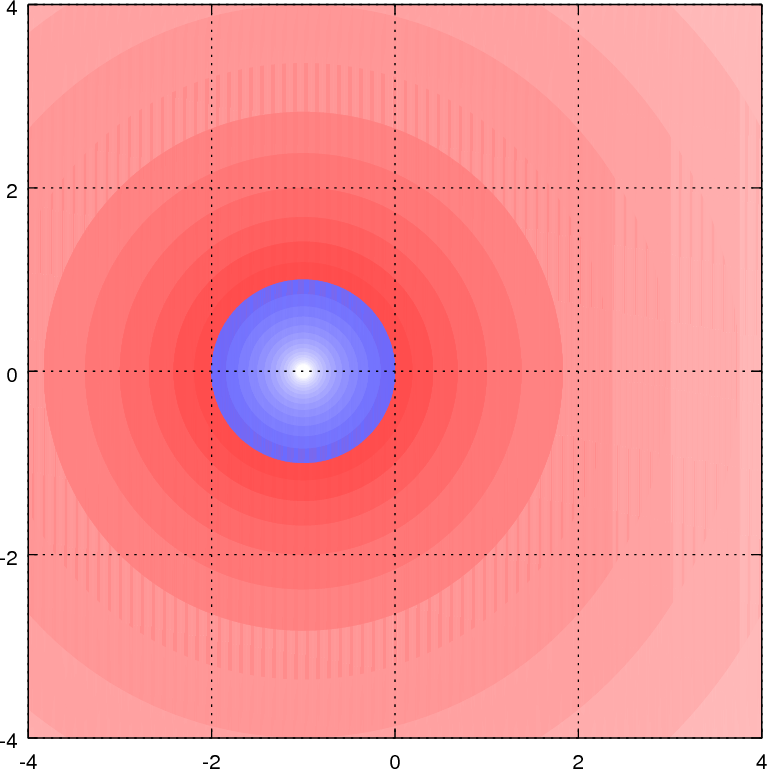
\includegraphics[width=.47\textwidth]{fig/stability-euler}
  \hfill
  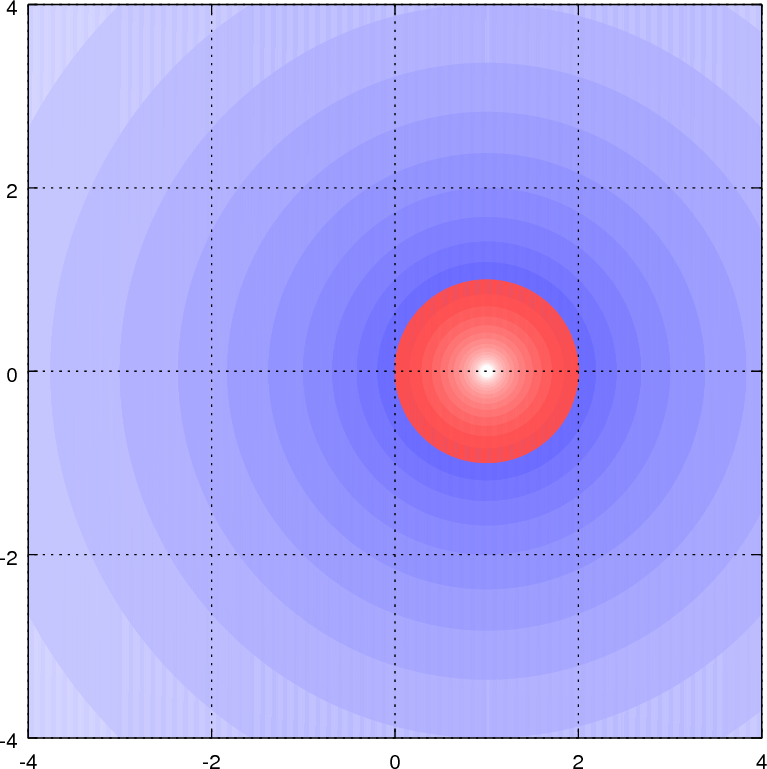
\includegraphics[width=.47\textwidth]{fig/stability-euler2}
  \caption{Stability regions of the explicit and implicit Euler
    methods (blue stable, red unstable)}
  \label{fig:implicit:stability-euler}
\end{figure}

\begin{Definition*}{a-stability}{A-stability}
  A method is called \define{A-stable}, if its stability region contains
  the left half-plane of $\C$, hence
  \begin{gather}
    \{ z \in \C | \ Re(z) \le 0 \} \subset S
  \end{gather}
\end{Definition*}

\begin{Definition*}{a-stability}{A-stability}
  A method is called \define{A-stable}, if its stability region contains
  the left half-plane of $\C$, hence
  \begin{gather}
    \{ z \in \C | \ Re(z) \le 0 \} \subset S
  \end{gather}
\end{Definition*}


% \begin{remark}
%   Der Begriff A-stabil wurde von Dahlquist bewusst neutral
%   gewählt. Insbesondere steht also A-Stabilität
%   \underline{\textbf{nicht}} für asymptotische Stabilität.
% \end{remark}

\begin{proof}
  Let $\{v_\ell\}_{\ell=1,\dots,d}$ be a basis of $\C^d$ consisting of
  eigenvectors of $A$. Such a basis exists since $A$ is
  diagonalizable. Let $y_0 = \sum_{\ell=1}^d \alpha^\ell v_\ell$ be
  the representation of $y_0$ in this basis. Furthermore, we introduce
  the representations $g_i = \sum_{\ell=1}^d \gamma_i^\ell
  v_\ell$. Then, we see that equations of the form
  \begin{gather*}
    g_i = y_0 + h \sum_{j=1}^s a_{ij} A g_i
  \end{gather*}
  decouple into
  \begin{gather*}
    \gamma_{i}^\ell = \alpha^\ell + h \sum_{j=1}^s a_{ij} \lambda_\ell \gamma_j^\ell.
  \end{gather*}
  Similarly, if $y_1 = \sum_{\ell=1}^d \eta^\ell v_\ell$ we have the separation
  \begin{gather*}
    y_1 = y_0 + h\sum_{i=1}^s b_i g_i
    \quad\longrightarrow\quad
    \eta^\ell = \alpha^\ell  + h\sum_{i=1}^s b_i \gamma_i^\ell.
  \end{gather*}
  Thus, instead of a vector valued problem, the method solves $d$
  decoupled scalar problems, inside and across time steps. But for each of the scalar problems, the definition of A-stability implies boundedness of the solution, if $\Re(\lambda_\ell) \le 0$.
\end{proof}

\begin{Theorem}{explicit-a-stability}
  \label{theorem:implicit:a-stability-erk}
  No explicit Runge-Kutta method is $A-stable$.
\end{Theorem}

\begin{proof}
  We show that for such methods $R(z)$ is a polynomial.  Then, the
  theorem follows immediately, it is known for polynomials, that the
  absolute value of its values goes to infinity, if the absolute value
  of the argument goes to infinity.
  
  From the equation~\eqref{eq:explicit:1b} follows $k_i = \lambda
  g_i$. If we insert that into the equation~\eqref{eq:explicit:1a},
  we obtain
  \begin{gather*}
    g_i = y_0 + h \sum_{j=1}^{i-1} \rka_{ij}k_j = y_0 + h\lambda
    \sum_{j=1}^{i-1} \rka_{ij} g_j.
  \end{gather*}
  With $g_1 = y_0$ and $z=h\lambda$ one has
  \begin{align*}
    g_2 &= y_0+ \rka_{21} z y_0 = (1+\rka_{21}z) y_0\\
    g_3 &= y_0 +  \rka_{32} z g_1 =  y_0 +  \rka_{32} z (1+\rka_{21} z) y_0 =
    (1+\rka_{32} z(1+\rka_{21} z)) y_0.
  \end{align*}
	Therefore one shows easily per induction that $k_j$ results as
	multiplication of a polynomial of order $j-1$ with $y_0$. 
  With formula~\eqref{eq:explicit:1c} we have that $R(z)$ is a
  polynomial of order $\rks-1$.
\end{proof}



\begin{remark}
  The notion of A-stability is only applicable to linear problems with
  diagonalizable matrices. Now we are considering its extension to
  nonlinear problems with monotonic right hand sides.
\end{remark}

\begin{Definition}{b-stability}
  A one-step method is called \define{B-stable}, if for monotonic
  initial value problems $u'=f(u)$ with arbitrary initial value $y_0$
  and $z_0$ there holds:
  \begin{equation}
    | y_1 - z_1 | \le | y_0 - z_0 |
  \end{equation}
  independent of the time step size $h$.
\end{Definition}

\begin{Definition}{b-stability}
  A one-step method is called \define{B-stable}, if for monotonic
  initial value problems $u'=f(u)$ with arbitrary initial value $y_0$
  and $z_0$ there holds:
  \begin{equation}
    | y_1 - z_1 | \le | y_0 - z_0 |
  \end{equation}
  independent of the time step size $h$.
\end{Definition}


\begin{proof}
  The theorem follows immediately by iterating over the definition of
  B-stability.
\end{proof}

\begin{corollary}
  A B-stable method applied to a linear differential equation with
  diagonalizable matrix $A$ is A-stable.
\end{corollary}

\begin{proof}
  Due to Lemma~\ref{lemma:linear-monotonic}, such a linear IVP is
  monotonic if and only if the eigenvalues of $A$ are in the right
  half-plane of $\C$. But then, the definition of B-stability implies
  $\abs{R(z)} \le 1$, and thus, the method is A-stable.
\end{proof}

\subsection{L-stability}

An undesirable feature of complex differentiable functions in the
context of stability of Runge-Kutta methods is the fact, that the
limit $\lim_{z\to \infty} R(z)$ is well-defined, independent of the
path chosen to approach this limit in the complex plane. Thus, for any
real number x, we have
\begin{gather}
  \lim_{x\to\infty} R(x) = \lim_{x\to\infty} R(ix).
\end{gather}

Thus, a method, which has exactly the left half-plane of $\C$ as its
stability domain, seemingly a desirable property, has the undesirable
property that components in eigenspaces corresponding to very large
negative eigenvalues, and thus decaying very fast in the continuous
problem, are decaying very slowly if such a method is applied.

This gave raise to the following notion of L-stability. We
nevertheless point out, that the L-stable methods are not always to be
considered better than A-stable ones, like it is not always necessary
to require A-stability. Judgment must be applied according to the
problem being solved.

\begin{Definition}{l-stability}
  An A-stable one-step method is called \define{L-stable}, if for its
  \putindex{stability function} there holds
  \begin{gather}
    \lim_{z\to\infty} \abs{R(z)} = 0.
  \end{gather}
\end{Definition}


%%%%%%%%%%%%%%%%%%%%%%%%%%%%%%%%%%%%%%%%%%%%%%%%%%%%%%%%%%%%%%%%%%%%%%
%%%%%%%%%%%%%%%%%%%%%%%%%%%%%%%%%%%%%%%%%%%%%%%%%%%%%%%%%%%%%%%%%%%%%%
\section{General Runge-Kutta methods}
%%%%%%%%%%%%%%%%%%%%%%%%%%%%%%%%%%%%%%%%%%%%%%%%%%%%%%%%%%%%%%%%%%%%%%
%%%%%%%%%%%%%%%%%%%%%%%%%%%%%%%%%%%%%%%%%%%%%%%%%%%%%%%%%%%%%%%%%%%%%%

\begin{intro}
  According to theorem~\ref{theorem:implicit:a-stability-erk}, ERK
  cannot be A- or B-stable. Thus, they are not suitable for long term
  integration of stiff IVP. The goal of this chapter is the study of
  methods not suffering from this limitation. The cure will be
  implicit methods, where stages may not only depend on
  known values from the past, but also on the value to be computed.
  
  We point out at the beginning of this chapter, that the main
  drawback of these methods is the fact that they require the solution
  of a typically nonlinear system of equations and thus involve much
  higher computational effort. Therefore, careful judgment should
  always be applied to determine whether a problem is really stiff or
  an implicit method is needed for other reasons.
\end{intro}

\begin{Definition}{rk}
  A \define{Runge-Kutta method} is a one-step method of the form
  \begin{subequations}
    \label{eq:implicit:1}
    \begin{xalignat}{2}
      \label{eq:implicit:1a}
      \rkg_i &= y_0 + h \sum_{j=1}^{\rks} \rka_{ij} k_j
      & i &= 1,\dots,\rks
      \\
      \label{eq:implicit:1b}
      k_i &= f(t_0+h \rkc_i, \rkg_i)
      & i &= 1,\dots,\rks
      \\
      \label{eq:implicit:1c}
      y_1 &= y_0 + h \sum_{i=1}^{\rks} \rkb_i k_i
    \end{xalignat}
  \end{subequations}
  The method is called
  \begin{description}
  \item[\textbf{ERK}] if $j \ge i\Rightarrow\rka_{ij} = 0$ (``explicit'')
    \index{Runge-Kutta method!explicit (ERK)|textbf}
  \item[\textbf{DIRK}] if $j>i\Rightarrow\rka_{ij} = 0$ (``diagonal implicit'')
    \index{Runge-Kutta method!diagonal implicit (DIRK)|textbf}
    \index{Diagonal implicit (DIRK)}
    \index{DIRK|see{Runge-Kutta method}}
  \item[\textbf{SDIRK}] if DIRK and $\forall i,j: \rka_{ii} =
    \rka_{jj}$ (``singly diagonal implicit'')
    \index{Runge-Kutta method!singly diagonal implicit (SDIRK)|textbf}
    \index{SDIRK|see{Runge-Kutta method}}
  \item[\textbf{IRK}] ``implicit'' in all other cases.
    \index{Runge-Kutta method!implicit (IRK)|textbf}
    \index{IRK|see{Runge-Kutta method}}
  \end{description}
\end{Definition}

%%% Local Variables: 
%%% mode: latex
%%% TeX-master: "../notes"
%%% End: 



\begin{example}[Two-stage SDIRK]
  Both SDIRK methods in table~\ref{tab:SDIRK2} are of 
  order three
  \begin{table}[htp]
    \centering
  \begin{gather}
    \def\arraystretch{1.5}
    \begin{array}{c|cc}
      \frac12 - \frac{\sqrt{3}}{6} & \frac12 - \frac{\sqrt{3}}{6} & 0 \\
      \frac12 + \frac{\sqrt{3}}{6} & \frac{\sqrt{3}}{3} & \frac12 - \frac{\sqrt{3}}{6} \\
      \hline
      & \frac12 & \frac12
    \end{array}
    \qquad
    \begin{array}{c|cc}
      \frac12 + \frac{\sqrt{3}}{6} & \frac12 + \frac{\sqrt{3}}{6} & 0 \\
      \frac12 - \frac{\sqrt{3}}{6} & -\frac{\sqrt{3}}{3} & \frac12 + \frac{\sqrt{3}}{6} \\
      \hline
      & \frac12 & \frac12
    \end{array}
  \end{gather}
    \caption{Two-stage SDIRK method of order 3}
    \label{tab:SDIRK2}
  \end{table}
\end{example}

% HW2, p. 40
\begin{Lemma}{stability-rk}
  The \putindex{stability function} of an $s$-stage Runge-Kutta method with
  coefficients
  \begin{gather*}
    A=
    \begin{pmatrix}
      \rka_{11} & \cdots & \rka_{1s}
      \\ \vdots & & \vdots \\
      \rka_{s1} & \cdots & \rka_{ss}
    \end{pmatrix},
    b =
    \begin{pmatrix}
      b_1 \\ \vdots \\ b_s
    \end{pmatrix},
  \end{gather*}
  is given by the two expressions
  \begin{gather}
    \label{eq:stability-rk:1}
    R(z) = 1+ z b^T \bigl(\identity-zA\bigr)^{-1}
    \begin{pmatrix}
      1\\\vdots\\1
    \end{pmatrix}
    = \frac{\operatorname{det}\left(\identity-zA+z
        \begin{pmatrix}
          b_1 & \cdots & b_s\\
          \vdots & & \vdots \\
          b_1 & \cdots & b_s
        \end{pmatrix}\right)
}{\operatorname{det}\bigl(\identity-zA\bigr)}
  \end{gather}
\end{Lemma}

%%% Local Variables:
%%% mode: latex
%%% TeX-master: "../notes"
%%% End:


\begin{proof}
  Entering $f(u) = \lambda u$ into the definition of the stages $g_i$,
  we obtain the linear system
  \begin{gather*}
    g_i = y_0 + h \sum_{j=1}^s a_{ij}\lambda g_j, \quad i=1,\dots,s.
  \end{gather*}
  In matrix notation with $z=h\lambda$, we obtain
  $(I-z A) g = (y_0,\dots,y_0)^T$, where $g$ is the vector
  $(g_1,\dots,g_s)^T$. Equally, we obtain
  \begin{align*}
    R(z) y_0 = y_1 &= y_0 + h \sum_{i=1}^s b_i \lambda g_i = y_0 + z
    b^T g\\
    &= y_0 + z b^T(I-z A)^{-1}
    \begin{pmatrix}
      y_0\\\vdots\\y_0
    \end{pmatrix}
    \\
    &= \left(1+z b^T(I-z A)^{-1}
      \begin{pmatrix}
        1\\\vdots\\1
      \end{pmatrix}
    \right) y_0.
  \end{align*}
  In order to prove the second representation, we write the whole Runge-Kutta method
  as a single system of equations of dimension $s+1$:
  \begin{gather*}
    \begin{pmatrix}
      I-z A & 0 \\
      -z b^T & 1
    \end{pmatrix}
    \begin{pmatrix}
      g \\ y_1
    \end{pmatrix}
    = y_0
    \begin{pmatrix}
      1\\\vdots\\1
    \end{pmatrix}.
  \end{gather*}
  Applying Cramer's rule yields the result.
\end{proof}

\begin{Example}{stability-examples-rk}
  Stability functions of the modified Euler method, of the classical
  Runge-Kutta method of order 4 and of the Dormand-Prince method of
  order 5 are
  \begin{align*}
    R_2(z) &= 1 + z + \tfrac{z^2}2 \\
    R_4(z) &= 1 + z + \tfrac{z^2}2 + \tfrac{z^3}{6} + \tfrac{z^4}{24}\\
    R_5(z) &= 1 + z + \tfrac{z^2}2 + \tfrac{z^3}{6} + \tfrac{z^4}{24}
             + \tfrac{z^5}{120} + \tfrac{z^6}{600}
  \end{align*}
  respectively. Their stability regions are shown in
  Figure~\ref{fig:implicit:stability-explicit-rk}.
\end{Example}

%%% Local Variables:
%%% mode: latex
%%% TeX-master: "../notes"
%%% End:

\begin{figure}[tp]
  \centering
  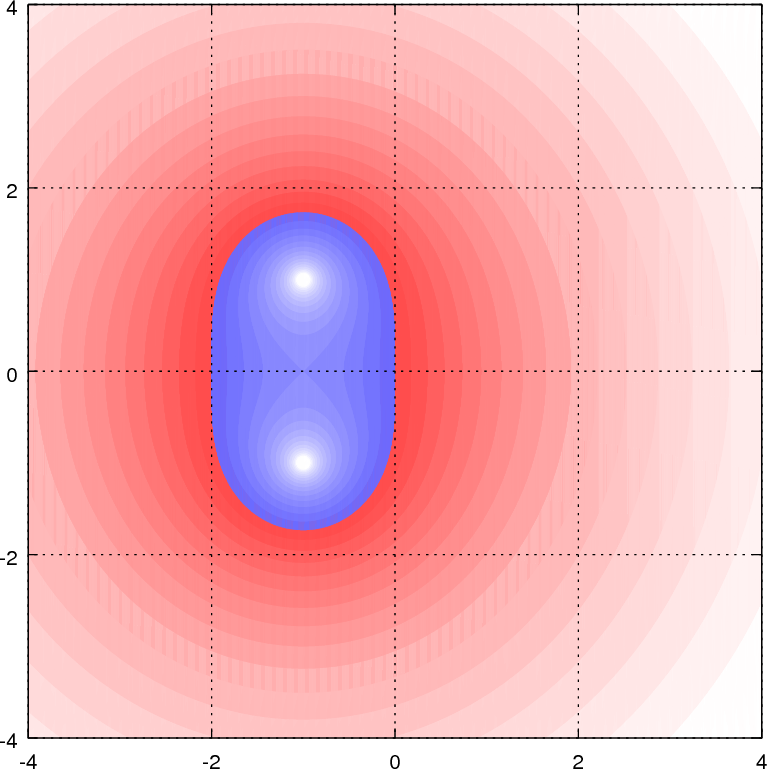
\includegraphics[width=.3\textwidth]{fig/stability-RK2}
  \hfill
  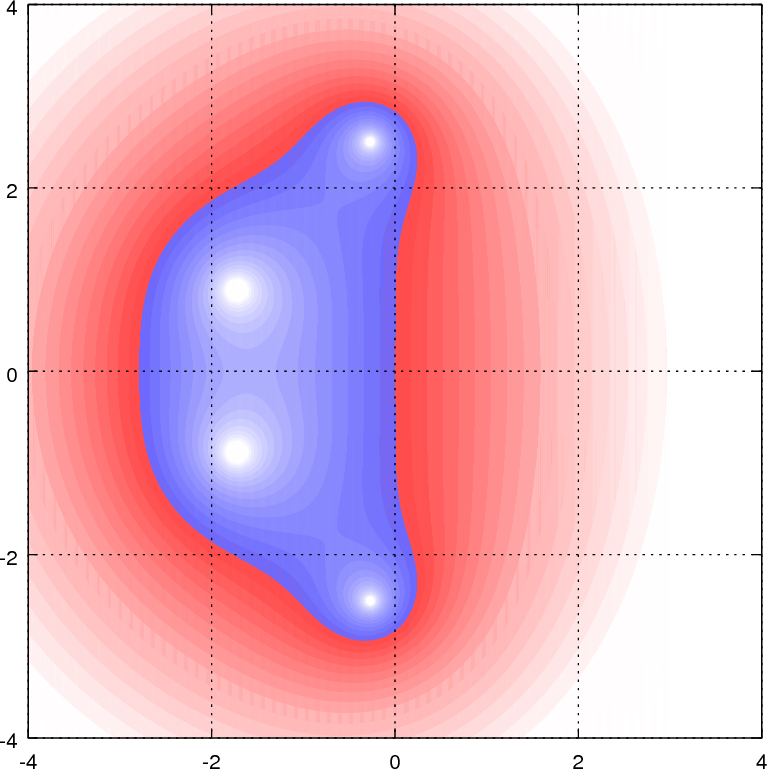
\includegraphics[width=.3\textwidth]{fig/stability-RK4}
  \hfill
  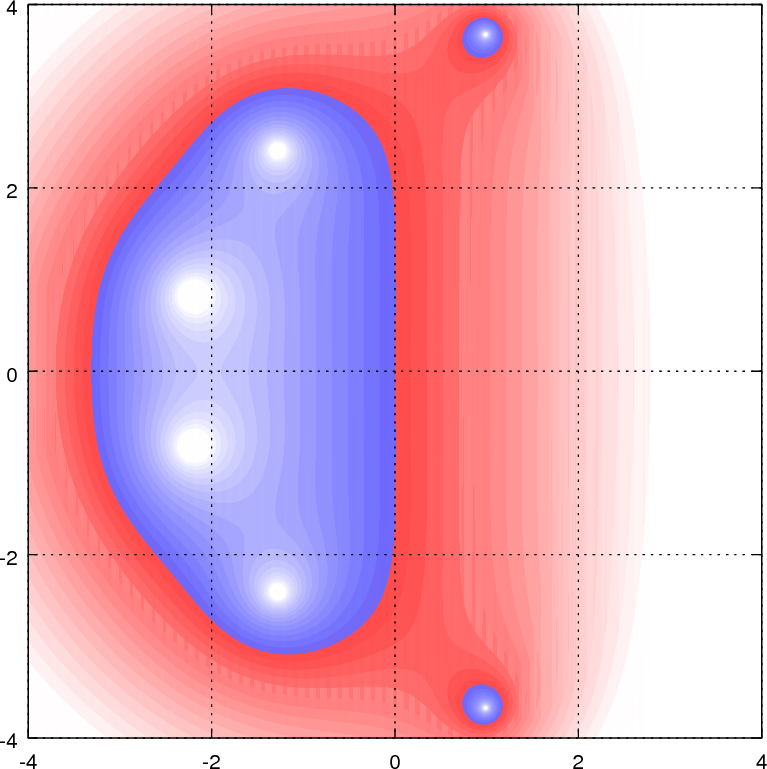
\includegraphics[width=.3\textwidth]{fig/stability-DOPRI5}
  \caption{Stability regions of the modified Euler method, the
    classical Runge-Kutta method of order 4 and the Dormand/Prince
    method of order 5 (blue stable, red unstable)}
  \label{fig:implicit:stability-explicit-rk}
\end{figure}

\begin{Definition}{theta-scheme}
  The $\theta$-scheme is the one-step method, defined for $\theta\in
  [0,1]$ by
  \begin{gather}
    \label{eq:theta:1}
    y_1 = y_0 + h \bigl((1-\theta) f(y_0) + \theta f(y_1)\bigr).
  \end{gather}
  It is an RKM with the Butcher Tableau
  \begin{gather}
    \label{eq:theta:2}
    \begin{array}{c|cc}
      0 & 0 & 0 \\
      1 & 1-\theta & \theta \\\hline
      & 1-\theta & \theta
    \end{array}.
  \end{gather}
  Three special cases are distinguished:
  \begin{center}
  \begin{tabular}{c|l}
    $\theta=0$ & explicit Euler method\\
    $\theta=1$ & implicit Euler method\\
    $\theta=1/2$ & Crank-Nicolson method
  \end{tabular}    
  \end{center}

  Furthermore, we define the variable $\theta$-scheme where $\theta$ is
  of the form
  \begin{gather*}
    \theta = \frac12 + \gamma h.
  \end{gather*}
\end{Definition}
%%% Local Variables:
%%% mode: latex
%%% TeX-master: "../notes"
%%% End:


\begin{Theorem}{theta-a-stability}
  The $\theta$-scheme is A-stable for $\theta\ge 1/2$. Furthermore, if
  there exists a constant $c$ such that $\theta-1/2 \le ch$, the
  method is consistent of second order.
\end{Theorem}

\begin{proof}
  Left as a homework question. Additionally, we show stability regions
  for different $\theta$ in Figure
  \begin{figure}[tp]
    \centering
    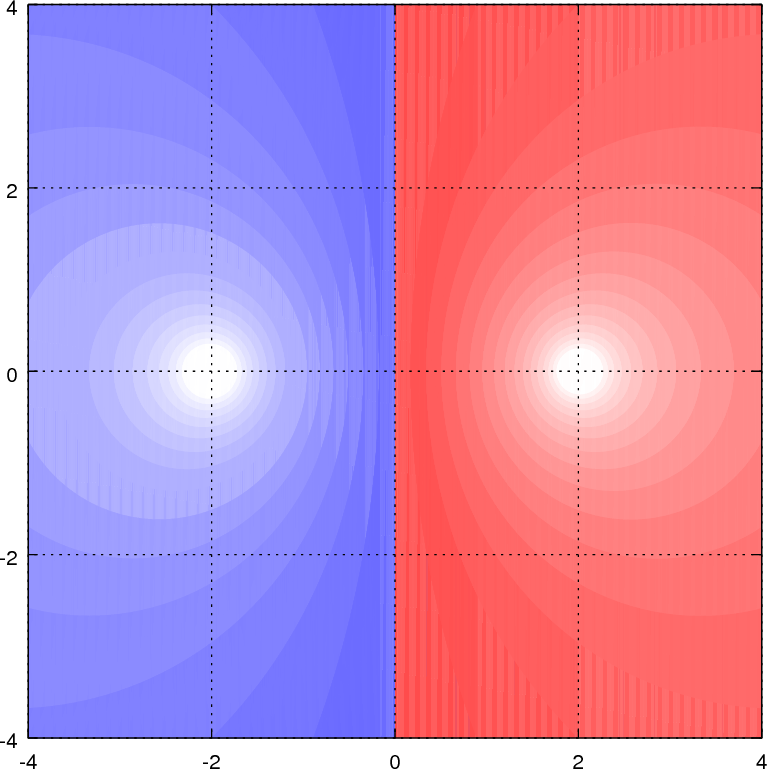
\includegraphics[width=.45\textwidth]{fig/stability-CR}
    \hfill
    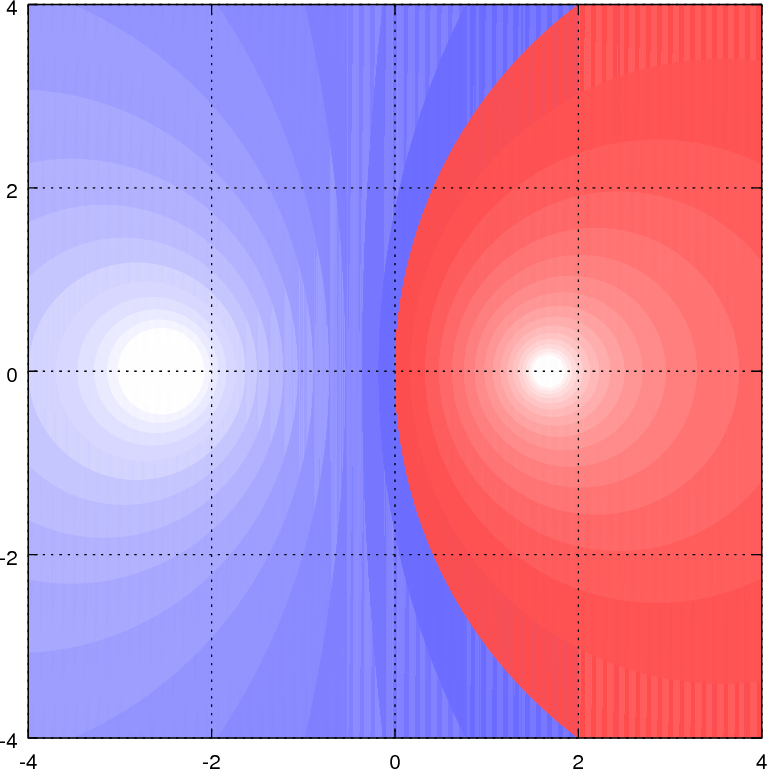
\includegraphics[width=.45\textwidth]{fig/stability-theta6}

    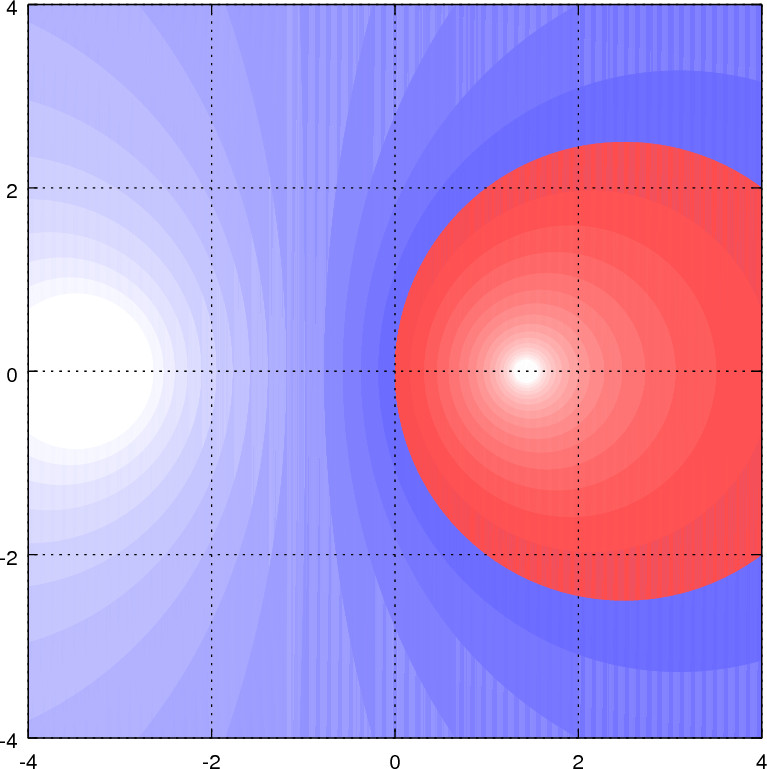
\includegraphics[width=.45\textwidth]{fig/stability-theta7}
    \hfill
    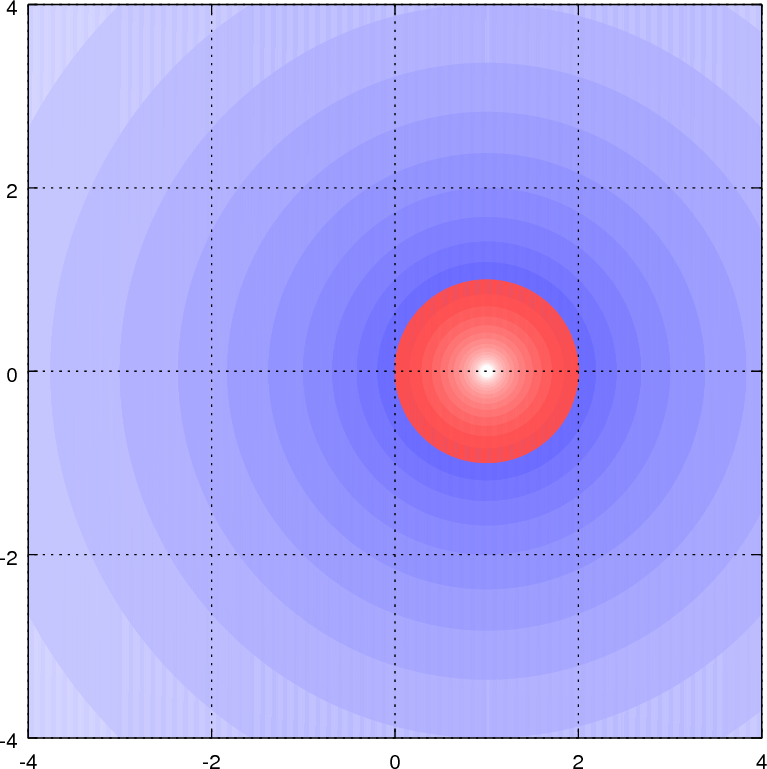
\includegraphics[width=.45\textwidth]{fig/stability-euler2}
    \caption{Stability regions of the $\theta$-scheme with
      $\theta=0.5$ (Crank-Nicolson), $\theta=0.6$, $\theta=0.7$, and
      $\theta=1$ (implicit Euler).}
    \label{fig:implicit:theta}
  \end{figure}
\end{proof}

\subsection{Existence and uniqueness of discrete solutions}

While it was clear that the steps of an explicit Runge-Kutta method
can always be executed, implicit methods require the solution of a
possibly nonlinear system of equations. The solvability of such a
system is not always clear. We will investigate several cases here:
First, Lemma~\ref{lemma:existence-implicit-1} based on a Lipschitz
condition on the right hand side. Since this result suffers from a
severe step size constraint, we add
Lemma~\ref{lemma:existence-implicit-2} for DIRK methods based on right
hand sides with a one-sided Lipschitz condition. Finally, we present
Theorem~\ref{theorem:existence-implicit-3} for general Runge-Kutta
methods with one-sided Lipschitz condition.

\begin{Lemma}{existence-implicit-1}{Cauchy 1824}
  Let $f:\R\times\C^d\to\C^d$ be continuous and satisfy the Lipschitz
  condition with constant $L$. If
  \begin{gather}
    \label{eq:existence-implicit-1:1}
    hL < \frac1{\max\limits_{i=1,\dots,s} \sum\limits_{j=1}^s \abs{a_{ij}}},
  \end{gather}
  then, for any $y_0$ the Runge-Kutta method~\eqref{eq:implicit:1} has a unique
  solution $y_1$.
\end{Lemma}

%%% Local Variables:
%%% mode: latex
%%% TeX-master: "../notes"
%%% End:


\begin{proof}
  We prove existence and uniqueness by a fixed-point argument. To this
  end, define the vectors
  $k^{(m)}=(k_1^{(m)},\dots,k_s^{(m)})^T\in \R^{s d}$ for $m=1,\dots$
  and the iteration $k^{(m)} = F(k^{(m-1)}$ by
  \begin{gather*}
    k_i^{(m)} = F_i(k^{(m-1)}) = f\left(
      t_0+c_i h, y_0+ h \sum_{j=1}^s a_{ij} k_j^{(m-1)}\right),
    \quad i=1,\dots,s.
  \end{gather*}
  Clearly the vector $k=(k_1,\dots,k_s)^T\in \R^{s d}$ of the
  Runge-Kutta method is a fixed-point of this iteration. Using on
  $\R^{s d}$ the norm $\norm{k} = \max_{i=1,\dots,s} \abs{k_i}$, where
  $\abs{.}$ is the regular Euclidean norm on $\R^d$, we obtain the
  estimate
  \begin{gather*}
    \norm{F(k_1)-F(k_2)}
    \le  \left(h L \max_{i=1,\dots,s} \sum_{j=1}^s \abs{a_{ij}}\right)
    \norm{k_1-k_2}.
  \end{gather*}
  Under assumption~\eqref{eq:existence-implicit-1:1}, the term in
  parentheses is strictly less than unity and thus, the mapping $F$ is
  a contraction. The \putindex{Banach fixed-point theorem} yields the
  unique existence.
\end{proof}

\begin{Lemma}{existence-implicit-2}
  Let $f:\R\times\C^d\to\C^d$ be continuous and satisfy the one-sided Lipschitz
  condition with constant $\nu$. If for $i=1,\dots,s$
  \begin{gather}
    \label{eq:existence-implicit-2:1}
    h\nu < \frac1{a_{ii}}
  \end{gather}
  then, for any $y_0$ the DIRK method~\eqref{eq:implicit:1} has a unique
  solution $y_1$.
\end{Lemma}

%%% Local Variables:
%%% mode: latex
%%% TeX-master: "../notes"
%%% End:


\begin{proof}
  The proof simplifies compared to the general case of an IRK, since
  each stage depends explicitly on the previous stages and implicitly
  only on itself.  Thus, we can write
  \begin{gather}
    \label{eq:implicit:18}
    g_i = y_0 + v_i + h a_{ii} f(g_i),
    \quad\text{with}\quad
    v_i = h \sum_{j=1}^{i-1} a_{ij} f(g_j).
  \end{gather}
  For linear IVP with diagonalizable matrix $A$, we have
  \begin{gather*}
    \left(I-ha_{ii} A\right) g_i = y_0 + v_i,
  \end{gather*}
  and assumption~\eqref{eq:existence-implicit-2:1} implies that all
  eigenvalues of $\left(I-ha_{ii} A\right)$ are positive, thus, the
  inverse exists and we obtain a unique solution.

  In the nonlinear case, we use a homotopy argument. To this end, we
  introduce the parameter $\tau\in [0,1]$ and set up the family of
  equations
  \begin{gather*}
    g(\tau) = y_0 + \tau v_i + h a_{ii} f(g(\tau)) + (\tau-1) h a_{ii} f(y_0).
  \end{gather*}
  For $\tau=0$ this equation has the solution $g(0) = y_0$, and for
  $\tau=1$ the solution $g(1) = g_i$. By showing, that
  $\frac{d}{d\tau}g$ is bounded, we conclude that a solution exists,
  since
  \begin{gather}
    \label{eq:implicit:19}
    g(1) = g(0) + \int_0^1 g'(s)\ds
  \end{gather}
  There holds
  \begin{gather*}
    g'(\tau) = v_i + h a_{ii} \partial_y f g'(\tau) + h a_{ii} f(y_0).
  \end{gather*}
  Thus
  \begin{align*}
    \abs{g'}^2 &= \scal(g',{v_i + h a_{ii}f(y_0)})
    + h a_{ii} \scal(g', \partial_y f g')\\
    & \le \abs{g'}\abs{v_i + h a_{ii} f(y_0)}
    + h a_{ii} \nu \abs{g'}^2.
  \end{align*}
  Here, we used that by the mean value theorem, there holds
  \begin{gather*}
    \scal(\partial_y f u,u) \le \nu \abs{u}^2,\quad\forall u\in \C^d.
  \end{gather*}
  We continue by stating that by assumption $1-h a_{ii} \nu > 0$ and thus
  \begin{gather*}
    \abs{g'} \le  \frac{\abs{v_i + h a_{ii} f(y_0)}}{1-h a_{ii} \nu}.
  \end{gather*}
  Thus, we have proved existence of the stages $g_i$. On the other
  hand$y_1$ is just a fixed linear combination of these values, such
  that it exists as well.
  Uniqueness follows immediately from A- or B-stability of the method.
\end{proof}

\begin{Theorem}{existence-implicit-3}
  Let be $f$ continuously differentiable and let it satisfy the 
  one-sided Lipschitz condition with constant $\nu$. If the
  Runge-Kutta matrix $A$ is invertible and if there is a vector
  $(d_1,\dots,d_s)$ with positive entries, such that
  \begin{gather}
    \label{eq:implicit:cond}
    h\nu < \frac{\scal(x,A^{-1}x)}{\sum\limits_{i=1}^s d_i x_i^2},
    \quad\forall x\in \R^s,
  \end{gather}
  then the nonlinear system~\ref{eq:implicit:1a} has a solution
  $(\rkg_1,...,\rkg_\rks)$.

\end{Theorem}
%%% Local Variables: 
%%% mode: latex
%%% TeX-master: "../notes"
%%% End: 


\begin{proof}
  We omit the proof here and refer to~\cite[Theorem IV.14.2]{HairerWanner10}
\end{proof}

% \begin{todo}
% In the following we want to discuss under which conditions a solution 
% for our IRK exists and is unique.
% For that we will need the help of some definitions:


% \begin{definition}
% 	We consider the inner product $\scal(u,v)_D = u^T Dv$,
%   where $D$ is a diagonal matrix with the entries $d_i > 0$. 
% 	We now denote with $\alpha_D(A^{-1})$ the largest number
%   $\alpha$ for which holds
%   \begin{gather}
%     \scal(u,A^{-1}u)_D \geq \alpha \scal(u,u)_D \qquad \forall u \in \R^\rks
%   \end{gather}

%   Futhermore we set
%   \begin{gather}
%     \alpha_0 (A^{-1}) = \sup_{D>0} \alpha_D (A^{-1})
%   \end{gather}
% \end{definition}



% \begin{theorem}[Existence of a solution for IRKs]
%   Let be f continuously differentiable and it satisfies the 
% 	one-sided Lipschitz condition with the Lipschitz constant $L$. If the
%   Runge-Kutta matrix $A$ is invertible and satisfies the condition
%   \begin{gather}
%     \label{eq:implicit:cond}
%     hL < \alpha_0 (A^{-1}),
%   \end{gather}
%   then the nonlinear system~\ref{eq:implicit:1a} has a solution
%   $(\rkg_1,...,\rkg_\rks)$.
% \end{theorem}



% \begin{remark}
% 	Now we examine the perturbation susceptibility of the solution of the IRK.
% 	For this purpose we use as before the notation
%   \begin{gather}
%     \begin{array}{lll}
%       || u ||_D & = \sqrt{u^TDu} = \sqrt{\langle u,u \rangle_D} & \ \ \ \forall u \in \R^\rks \\
%       || g ||_D & = \sqrt{g^T(D\otimes I)g} & \ \ \ \forall g \in \R^{\rks n}
%     \end{array}
%   \end{gather}
% \end{remark}


% \begin{theorem}
%   \label{theorem:implicit:perturb}
%   Given $\rkg_i$ and $y_1$ as in ~\ref{eq:implicit:1a} and ~\ref{eq:implicit:1c} and the perturbed values $\hat{\rkg}_i$ and $\hat{y}_1$ are defined as follows
%   \begin{gather}
%     \begin{split}
%       \hat{\rkg}_i & = y_0 + h \sum\limits_{j=1}^\rks \rka_{ij} f(x_0 + \rkc_j h, \hat{\rkg}_j) + \delta_i \\
%       \hat{y}_1 & = y_0 + h \sum\limits_{j=1}^\rks \rkb_j f(x_0 + \rkc_j h, \hat{\rkg}_j) \\
%     \end{split}
%   \end{gather}

%   If the Runge-Kutta matrix A is invertible, the differential equation 
% 	satisfies the one-sided Lipschitz condition and for a positive diagonal
% 	matrix D holds $hL<\alpha_D(A^{-1})$, then we have the estimates
%   \begin{gather}
%     \begin{split}
%       ||\hat{\rkg}-\rkg||_D & \le \frac{||A^{-1}||_D}{\alpha_D(A^{-1})-hL}||\delta||_D \\
%       ||\hat{y}_1 - y_1|| & \le ||b^TA^{-1}||_D \left( 1+\frac{||A^{-1}||_D}{\alpha_D(A^{-1})-hL} \right) ||\delta||_D \\
%     \end{split}
%   \end{gather}

%   where $\rkg = (\rkg_1,...,\rkg_\rks)^T$, $\hat{\rkg}=(\hat{\rkg}_1,...,\hat{\rkg}_\rks)^T$ and $\delta=( \delta_1,...,\delta_\rks)^T$.
% \end{theorem}


%  \begin{proof}
% % \begin{todo}
% %     \cite[IV.14.3]{HairerWanner10}
% % \end{todo}
%  \end{proof}


% \begin{theorem}[Uniqueness of the solution for IRKs]
%   For a differential equation, which satisfies the Lipschitz conditions,
%   the following holds true: a Runge-Kutta method has maximal one solution
% 	if its matrix $A$ is invertible 
%   and the condition $~\ref{eq:implicit:cond}$ is satisfied.
% \end{theorem}


% \begin{proof}
%   Set $\delta = 0$ in $~\ref{theorem:implicit:perturb}$.
% \end{proof}
% \end{todo}

\begin{Definition*}{simplifying-conditions}{Simplifying order conditions}
% HNW p. 208
  \index{order condition (IRK)}
  Define the conditions
  \begin{subequations}
    \label{eq:implicit:order}
    \begin{xalignat}{3}
      \label{eq:implicit:8}
      B(\xi):&&
      \sum_{i=1}^s \rkb_i \rkc_i^{q-1} &= \frac1{q}
      &&
      \begin{array}{r@{\,}l}
        q&=1,\ldots,\xi
      \end{array}
      \\
      \label{eq:implicit:9}
      C(\xi):&& \sum_{j=1}^s \rka_{ij} \rkc_j^{q-1} &= \frac{\rkc_i^{q}}{q}
      &&
      \begin{array}{r@{\,}l}
        q&=1,\ldots,\xi\\
        i&=1,\dots,\rks
      \end{array}
      \\
      \label{eq:implicit:11}
      D(\xi):&&
      \sum_{i=1}^s \rkb_i \rka_{ij} \rkc_i^{q-1} &=
      \frac{\rkb_j}{q}(1-\rkc_j^{q})
      &&
      \begin{array}{r@{\,}l}
        q&=1,\ldots,\xi\\
        j&=1,\dots,\rks
      \end{array}
    \end{xalignat}
  \end{subequations}
\end{Definition*}

%%% Local Variables: 
%%% mode: latex
%%% TeX-master: "../notes"
%%% End: 

\begin{Definition*}{simplifying-conditions}{Simplifying order conditions}
% HNW p. 208
  \index{order condition (IRK)}
  Define the conditions
  \begin{subequations}
    \label{eq:implicit:order}
    \begin{xalignat}{3}
      \label{eq:implicit:8}
      B(\xi):&&
      \sum_{i=1}^s \rkb_i \rkc_i^{q-1} &= \frac1{q}
      &&
      \begin{array}{r@{\,}l}
        q&=1,\ldots,\xi
      \end{array}
      \\
      \label{eq:implicit:9}
      C(\xi):&& \sum_{j=1}^s \rka_{ij} \rkc_j^{q-1} &= \frac{\rkc_i^{q}}{q}
      &&
      \begin{array}{r@{\,}l}
        q&=1,\ldots,\xi\\
        i&=1,\dots,\rks
      \end{array}
      \\
      \label{eq:implicit:11}
      D(\xi):&&
      \sum_{i=1}^s \rkb_i \rka_{ij} \rkc_i^{q-1} &=
      \frac{\rkb_j}{q}(1-\rkc_j^{q})
      &&
      \begin{array}{r@{\,}l}
        q&=1,\ldots,\xi\\
        j&=1,\dots,\rks
      \end{array}
    \end{xalignat}
  \end{subequations}
\end{Definition*}

%%% Local Variables: 
%%% mode: latex
%%% TeX-master: "../notes"
%%% End: 


\begin{proof}
  For the proof, we refer to~\cite[Ch. II, Theorem
  7.4]{HairerNorsettWanner93}. Here, we only observe, that
  \begin{gather*}
    \int_0^1 x^{q-1} \dx = \frac1{q}, \qquad
    \int_0^{c_i} x^{q-1} \dx = \frac{c_i q^{q}}{q}.
  \end{gather*}
  If we now insert the function $x$ at the places $c_i$ into the
  quadrature formula with the quadrature weights $\rkb_i$, then we
  obtain~\eqref{eq:implicit:8}. Similarly we get~\eqref{eq:implicit:9}, if we insert the value $x^{q}/q$ at
  the places $c_i$ from the quadrature formula with weights
  $\rka_{ij}$ for $j=1,\dots,s$. In both cases we carry this out for
  all momomials until the desired degree is reached.  Due to linearity
  of the formulas the exactness holds for all polynomials until this
  degree.
\end{proof}

%%%%%%%%%%%%%%%%%%%%%%%%%%%%%%%%%%%%%%%%%%%%%%%%%%%%%%%%%%%%%%%%%%%%%%
%%%%%%%%%%%%%%%%%%%%%%%%%%%%%%%%%%%%%%%%%%%%%%%%%%%%%%%%%%%%%%%%%%%%%%
\section{Methods based on quadrature and B-stability}
%%%%%%%%%%%%%%%%%%%%%%%%%%%%%%%%%%%%%%%%%%%%%%%%%%%%%%%%%%%%%%%%%%%%%%
%%%%%%%%%%%%%%%%%%%%%%%%%%%%%%%%%%%%%%%%%%%%%%%%%%%%%%%%%%%%%%%%%%%%%%

\subsection{Gauss-, Radau-, and Lobatto-quadrature}

\begin{intro}
  In this subsection, we review some of the basic facts of quadrature
  formulas based on orthogonal polynomials.
\end{intro}

\begin{Lemma}{gauss-quadrature}
  A Gauß quadrature formula with $n$ points is exact for polynomials
  of degree $2n-1$. A Radau quadrature formula with $n$ points is
  exact for polynomials of degree $2n-2$. A Lobatto quadrature formula
  with $n$ points is exact for polynomials of degree $2n-3$.
\end{Lemma}
\begin{Definition}{radau-lobatto-quadrature}
  The \define{Radau quadrature} formulas use one end point of the interval
  $[0,1]$ and the roots of orthogonal polynomials of degree $n-1$ as
  their abscissas. We distinguish left and right Radau quadrature
  formulas, depending on which end is included. \define{Lobatto quadrature}
  formulas use both end points and the roots of a polynomial of degree
  $n-2$. In all three cases, the abscissas are the roots of the polynomials
  \begin{xalignat}2
    \text{Radau}&\text{ left}
    & p_n(x) &= \frac{d^{n-1}}{dx^{n-1}}\bigl(x^n(x-1)^{n-1}\bigr), \\
    \text{Radau}&\text{ right}
    & p_n(x) &= \frac{d^{n-1}}{dx^{n-1}}\bigl(x^{n-1}(x-1)^{n}\bigr), \\
    \text{Lobatto}&
    & p_n(x) &= \frac{d^{n-2}}{dx^{n-2}}\bigl(x^{n-1}(x-1)^{n-1}\bigr).
  \end{xalignat}
\end{Definition}

\begin{Lemma}{gauss-quadrature}
  A Gauß quadrature formula with $n$ points is exact for polynomials
  of degree $2n-1$. A Radau quadrature formula with $n$ points is
  exact for polynomials of degree $2n-2$. A Lobatto quadrature formula
  with $n$ points is exact for polynomials of degree $2n-3$.
\end{Lemma}

\subsection{Collocation methods}
\begin{intro}
  An alternative to solving IVP in individual points in time, is to
  develop methods, which first approximate the solution function
  through a easier function. For example this could be a polynomial.
  
  Polynomials are especially suitable for the computation with
  computers.  On the other hand we know already that they cause
  problems for instance by the interpolation of large intervals.
  Therefore we apply them not on the entire interval but rather on
  subintervals. The subintervals correspond obviously to our time
  steps, which we used until now.
\end{intro}

\begin{Lemma}{collocation}
% HKW p. 212
  A $\rks$-stage collocation method with the points $\rkc_1$
  to $\rkc_\rks$ defines a Runge-Kutta method of
  definition~\ref{definition:rk} with the coefficients $\rkc_i$ and
  \begin{gather}
  \label{eq:implicit:kolkoef}
    \rka_{ij} =  \int_0^{\rkc_i} L_j(t)\, \diffd t,
    \qquad
    \rkb_i =\int_0^1 L_j(t)\, \diffd t.
  \end{gather}
  Here is $L_j(t)$ Lagrange's interpolation polynomial to point $\rkc_j$
  and to the point set $\{\rkc_1,\dots,\rkc_\rks\}$:
  \begin{gather*}
    L_j(t) = \prod_{\substack{k=1\\k\neq j}}^\rks \frac{t-\rkc_k}{\rkc_j-\rkc_k}.
  \end{gather*}
\end{Lemma}

%%% Local Variables: 
%%% mode: latex
%%% TeX-master: "../notes"
%%% End: 

\begin{Lemma}{collocation}
% HKW p. 212
  A $\rks$-stage collocation method with the points $\rkc_1$
  to $\rkc_\rks$ defines a Runge-Kutta method of
  definition~\ref{definition:rk} with the coefficients $\rkc_i$ and
  \begin{gather}
  \label{eq:implicit:kolkoef}
    \rka_{ij} =  \int_0^{\rkc_i} L_j(t)\, \diffd t,
    \qquad
    \rkb_i =\int_0^1 L_j(t)\, \diffd t.
  \end{gather}
  Here is $L_j(t)$ Lagrange's interpolation polynomial to point $\rkc_j$
  and to the point set $\{\rkc_1,\dots,\rkc_\rks\}$:
  \begin{gather*}
    L_j(t) = \prod_{\substack{k=1\\k\neq j}}^\rks \frac{t-\rkc_k}{\rkc_j-\rkc_k}.
  \end{gather*}
\end{Lemma}

%%% Local Variables: 
%%% mode: latex
%%% TeX-master: "../notes"
%%% End: 


\begin{proof}
  The polynomial $y'(t)$ is of degree $\rks-1$ and therefore uniquely
  defined through $\rks$ interpolation conditions in
  equation~\eqref{eq:implicit:12}.  We set $y'(x_0 + \rkc_i h) =
  f\bigl(t_0+\rkc_i h, y(t_0+\rkc_i h)\bigr) = k_i$, such that we have
  \begin{gather}
    y'(x_0+t h) = \sum\limits_{j=1}^\rks k_j \cdot L_j(t)
  \end{gather}
  with the Lagrange interpolation polynomial $L_j(t)$.
  By integration we obtain:
  \begin{gather}
    g_i = y(x_0 + \rkc_i h)
    = y_0 + h \int\limits_0^{\rkc_i} y'(x_0 + t h) \dt
    = y_0+h \sum_{j=1}^s k_j \int_0^{\rkc_i} L_j(t)\dt,
  \end{gather}
  which defines the coefficients $\rka_{ij}$ by comparison with
  ~\eqref{eq:implicit:1a}.  If we integrate to one instead of until
  $c_i$, then we obtain the coefficients $\rkb_j$ by comparison
  with~\eqref{eq:implicit:1c}.
\end{proof}


\begin{Lemma}{collocation-equivalence}
% HKW p. 212
  An implicit $\rks$-stage Runge-Kutta method of order $\rks$ or
  higher, with pairwise different support points $\rkc_i$ is a
  collocation method if and only if simplifying condition $C(s)$
  in~\eqref{eq:implicit:9} is satisfied. In other words, an
  $\rks$-stage method is a collocation method as soon as all the
  ``quadrature formulas'' involved are of order at least $\rks$.
\end{Lemma}

%%% Local Variables: 
%%% mode: latex
%%% TeX-master: "../notes"
%%% End: 


\begin{proof}
  Condition $C(s)$ from~\eqref{eq:implicit:9} results in
  $s^2$ interpolation conditions for $s^2$ coefficients $a_{ij}$.
  Therefore this coefficients are defined uniquely. On the other
  hand~\eqref{eq:implicit:9} yields for $q<s$:
  \begin{gather*}
    \sum_{j=1}^s \rka_{ij} \rkc_j^q = \frac{\rkc_i^{q+1}}{q+1} =
    \int_{0}^{\rkc_i} t^q \dt.
  \end{gather*}
  As a consequence of linearity we have
  \begin{gather*}
    \sum_{j=1}^s \rka_{ij} p(\rkc_i) = \int_{0}^{\rkc_i} p(t)
    \dt,\qquad\forall p\in \Pol_{s-1}.
  \end{gather*}
  Applying this to Lagrange interpolation polynomials $L_j(t)$, we
  obtain the coefficients of equation~\eqref{eq:implicit:kolkoef},
  which were in turn computed from the collocation polynomial.
\end{proof}

\begin{Theorem}{collocation-order}
  Consider a collocation method with $s$ pairwise different support
  points $\rkc_i$ and define
  \begin{gather}
    \label{eq:implicit:14}
    \pi(t) = \prod_{i=1}^\rks (t-c_i).  
  \end{gather}
  If $\pi(t)$ is orthogonal on $[0,1]$ to all polynomials of degree
  $r-1$ for $r\le s$, then the collocation
  method~\eqref{eq:implicit:13} is of order $p=s+r$.
\end{Theorem}


%%% Local Variables: 
%%% mode: latex
%%% TeX-master: "../notes"
%%% End: 


\begin{proof}
  The condition on $\pi$ implies that the quadrature rule is exact for
  polynomials of degree $s+r-1$, thus $B(s+r)$ holds.
  We have already shown in the proof of
  Lemma~\ref{lemma:collocation-equivalence}, that $C(s)$
  holds. Therefore, it remains to show $D(r)$.

  First, we observe that first by $C(s)$ and then by $B(s+r)$ for
  any $p<s$ and $q\le r$ there holds
  \begin{gather*}
    \sum_{i=1}^s\sum_{j=1}^s b_i c_i^{q-1} a_{ij} c_j^{p-1}
    = \frac1p \sum_{i=1}^s b_i c_i^{p+q-1}
    = \frac1{p(p+q)}.
  \end{gather*}
  Furthermore, since $B(s+r)$ we have for the same $p$ and $q$:
  \begin{gather*}
    \frac1q\sum_{j=1}^s\bigl(b_j c_j^{p-1} - b_j c_j^{p+q-1}\bigr)
    = \frac1q\left(\frac1q - \frac1{p+q}\right)
    = \frac1{p(p+q)}.
  \end{gather*}
  Subtracting these two and integrating the last result yields
  \begin{gather*}
    0 = \frac{1}{p(p+q)}-\frac{1}{p(p+q)} =
    \sum_{j} c_j^{p-1} \underbrace{\left(
      \sum_i b_i c_i^{q-1}a_{ij} - \frac1q b_j \bigl(1-c_j^q\bigr)
    \right)}_{:= \xi_i}.
  \end{gather*}
  This holds for $p=1,\dots,s-1$ and thus amounts to a homogeneous,
  linear system in the variables $\xi_i$. Thus, $\xi_i=0$ and the
  theorem holds.  \marginpar{Oops!}
%%% Todo!
\end{proof}

\begin{corollary}
  An $\rks$-stage collocation method is at least of order
  $\rks$ and at most of order $2\rks$.
\end{corollary}

\begin{proof}
  The polynomial $\pi(t)$ in~\eqref{eq:implicit:14} is of degree
  $\rks$. As a result it can be orthogonal on all polynomials of
  degree $\rks-1$ in the best case.  Otherwise it would be orthogonal
  to itself.  The transformed Legendre polynomial of degree $\rks$ on
  the interval $[0,1]$ satisfies this condition and
  theorem~\ref{theorem:collocation-order} holds true with
  $r=s$. On the other hand $\pi(t)$ is not orthogonal on the
  constants. In this case the theorem holds true with $r=0$.
\end{proof}


\begin{Theorem}{collocation-continuous}
  \index{Runge-Kutta method!continuous} The collocation polynomial
  $y(t)$, defined through an $\rks$-stage collocation method of the
  form~\eqref{eq:implicit:13}, defines a continuous Runge-Kutta method
  of order $s$. This means for the difference of the exact solution
  $u(t)$ of the initial value problem and the collocation polynomial
  $y(t)$ we get the estimate
  \begin{gather}
    \label{eq:implicit:15}
    \abs{u(t)-y(t)} \le C h^{s+1}.
  \end{gather}
  Additionally we obtain for the derivatives of order $k\le s$ the
	estimate
  \begin{gather}
    \label{eq:implicit:16}
    \abs{u^{(k)}(t)-y^{(k)}(t)} \le C h^{s+1-k}.
  \end{gather}
\end{Theorem}


\begin{proof}
  We immediately obtain the statement for the derivatives through
  the fact, that the polynomial $y'(t)$ interpolates the function $u'(t)$ 
  in the points $\rkc_i$. We receive the error estimate for $y(t)$
  by integration of the initial value. 
\end{proof}


\begin{Definition}{gauss-collocation}
  \defindex{collocation method!Gauß} An $\rks$-stage
  \define{Gauß-Collocation method} is a collocation method, where the
  collocation points are the set of $\rks$ Gauß points in the interval
  $[0,1]$, namely the roots of the Legendre polynomial of degree $\rks$.
\end{Definition}


\begin{example}
  The two- and three-stage Gauß-Collocation methods were described by
  Hammer and Hollingsworth or\ Kuntzmann and Butcher. 
	Their Butcher tables are (c.f.~\cite[Tables
  7.3, 7.4]{HairerNorsettWanner93}):
  \begin{table}[tp]
    \begin{minipage}[t]{.49\linewidth}
      \begin{gather*}
  \def\arraystretch{1.5}
  \begin{array}{c|cc}  
    \frac{3-\sqrt3}{6} & \frac14 & \frac14-\frac{\sqrt3}{6}
    \\
    \frac{3+\sqrt3}{6} & \frac14+\frac{\sqrt3}{6} & \frac14
    \\\hline
                       & \frac12 & \frac12
  \end{array}
\end{gather*}

%%% Local Variables:
%%% mode: latex
%%% TeX-master: "../notes"
%%% End:

    \end{minipage}
    \begin{minipage}[t]{.49\linewidth}
      \begin{gather*}
  \def\arraystretch{1.5}
  \begin{array}{c|ccc}
    \frac{5-\sqrt{15}}{10}
    & \frac{5}{36}
    & \frac29 - \frac{\sqrt{15}}{15}
    & \frac{5}{36} - \frac{\sqrt{15}}{30}
    \\
    \frac12
    & \frac{5}{36} + \frac{\sqrt{15}}{24}
    & \frac29
    & \frac{5}{36} - \frac{\sqrt{15}}{24}
    \\
    \frac{5+\sqrt{15}}{10}
    & \frac{5}{36} + \frac{\sqrt{15}}{30}
    & \frac29 + \frac{\sqrt{15}}{15}
    & \frac{5}{36}
    \\\hline
    & \frac{5}{18} & \frac49 & \frac{5}{18}
  \end{array}  
\end{gather*}

%%% Local Variables:
%%% mode: latex
%%% TeX-master: "../notes"
%%% End:
      
    \end{minipage}
    \caption{Gauß-Collocation methods with two and three collocation points}
    \label{tab:gauss-collokation-2-3}
  \end{table}
\end{example}

\begin{Theorem}{gauss-consistency}
  The $\rks$-stage Gauß-collocation method is consistent of order
  $2\rks$ and thus of optimal order.
  
  The $\rks$-stage Radau- and Lobatto-collocation methods are of
  orders $2s-1$ and $2s-2$, respectively.
\end{Theorem}


%%% Local Variables:
%%% mode: latex
%%% TeX-master: "../notes"
%%% End:


\begin{proof}
  Gauß quadrature is exact for polynomials of degree $2s-1$ and we
  have that $\pi$ in Theorem~\ref{theorem:collocation-order} is of
  order $s$. Therefore, the same theorem concludes that the method is
  of order $2s$. The same proof applies to Radau- and Lobatto-
  quadrature rules with their reduced orders.
\end{proof}

\begin{Theorem}{gauss-stability}
% HW p. 181 Example 12.3
  Collocation methods with Gauß-, Radau- and Lobatto-quadrature are
  \putindex{B-stable}. The stability region of Gauß-collocation is
  exactly the left half-plane of $\C$.
\end{Theorem}

%%% Local Variables:
%%% mode: latex
%%% TeX-master: "../notes"
%%% End:


\begin{proof}
  We only prove the theorem for Gauß-collocation, where the proof is
  simple and instructive. The proof for Radau- and Lobatto-collocation
  can be found in~\cite{HairerWanner10}.

  Let be $y(t)$ and $z(t)$ the collocation polynomials according
  to~\eqref{eq:implicit:13} with respect to initial values $y_0$ or
  $z_0$. Analogous to the proof of
  theorem~\ref{theorem:stability-monotonic} we introduce the auxiliary
  function $m(t) = | z(t)-y(t)|^2$. In the collocation points
  $\xi_i = t_0 + \rkc_i h$, there holds
  \begin{multline}
    \label{eq:implicit:20}
    m'(\xi_i) = 2 \Re\left<
      z'(t)-y'(t),z(t)-y(t)\right>
    \\
    = 2 \Re\left<f(\xi_i,z(\xi_i)) -
      f(\xi_i,y(\xi_i)),z(t)-y(t)\right> \le 0. 
  \end{multline}
  Since Gauß quadrature is exact for polynomials of degree $2s-1$, we have:
  \begin{multline*}
    |z_1-y_1|^2 = m(t_0+h) = m(t_0) + \int_{t_0}^{t_0+h} m'(t)\dt
    \\
    = m_0+h \sum_{i=1}^s b_i m'(\xi_i) \le m(t_0) =  |z_0-y_0|^2.
  \end{multline*}
  Applying this argument to $f(t,u) = \lambda u$, we see 
  $A$, we see from~\eqref{eq:implicit:20} that
  \begin{gather*}
    m'(t) = 2\Re(\lambda) \abs{z(t)-y(t)}^2,
  \end{gather*}
  which proves the statement about the stability domain.
\end{proof}

\begin{remark}
  The Radau-collocation methods with right end point of the interval
  $[0,1]$ included in the quadrature set are L-stable. The stability
  regions of the first three are shown in
  Figure~\ref{fig:radau-collocation}. The corresponding Butcher
  tableaus are in Table~\ref{tab:radau-collokation-2-3}.
\end{remark}
\begin{figure}[tp]
  \centering
  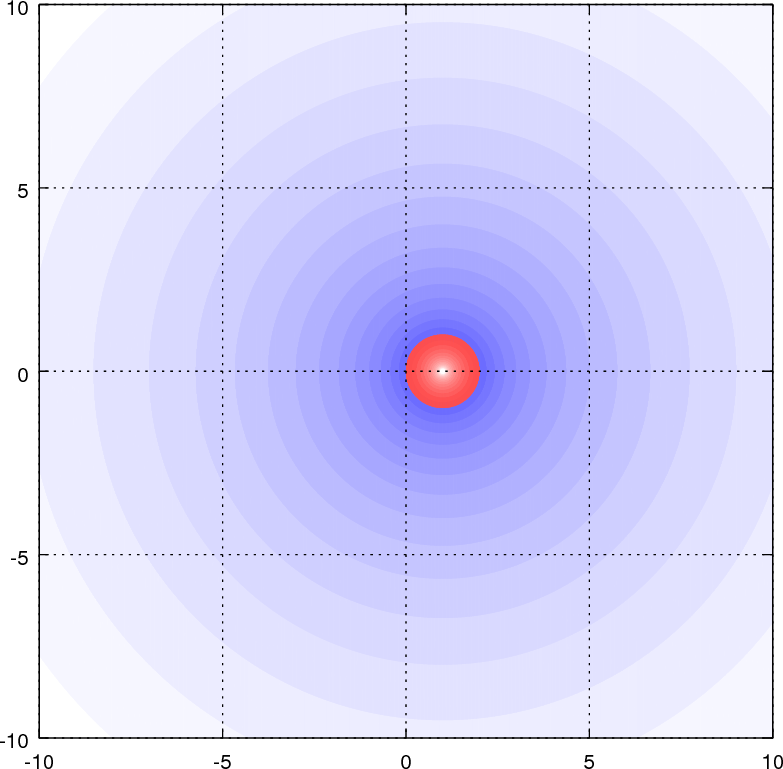
\includegraphics[width=.3\textwidth]{fig/stability-radau1}
  \hfill
  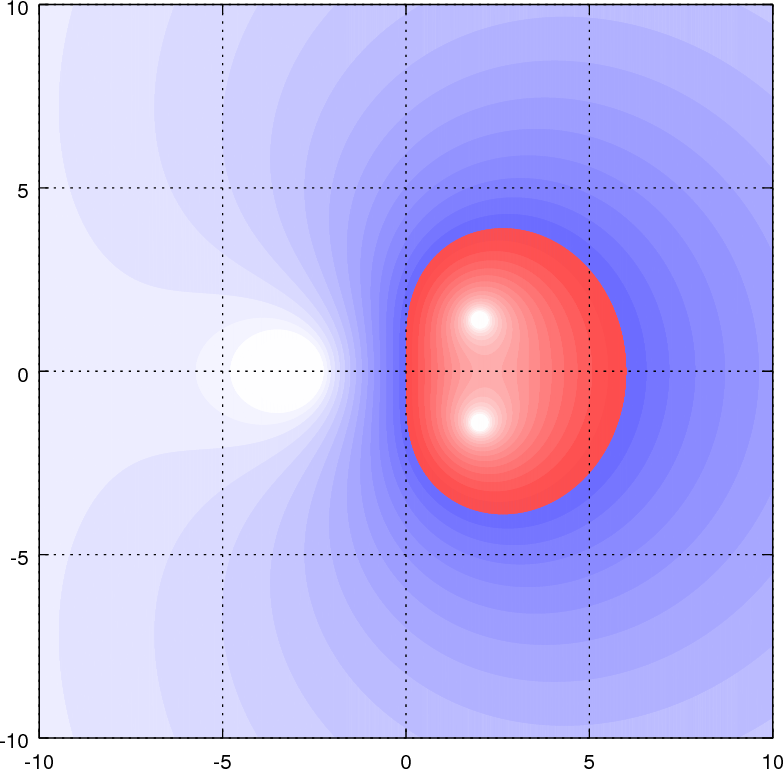
\includegraphics[width=.3\textwidth]{fig/stability-radau2}
  \hfill
  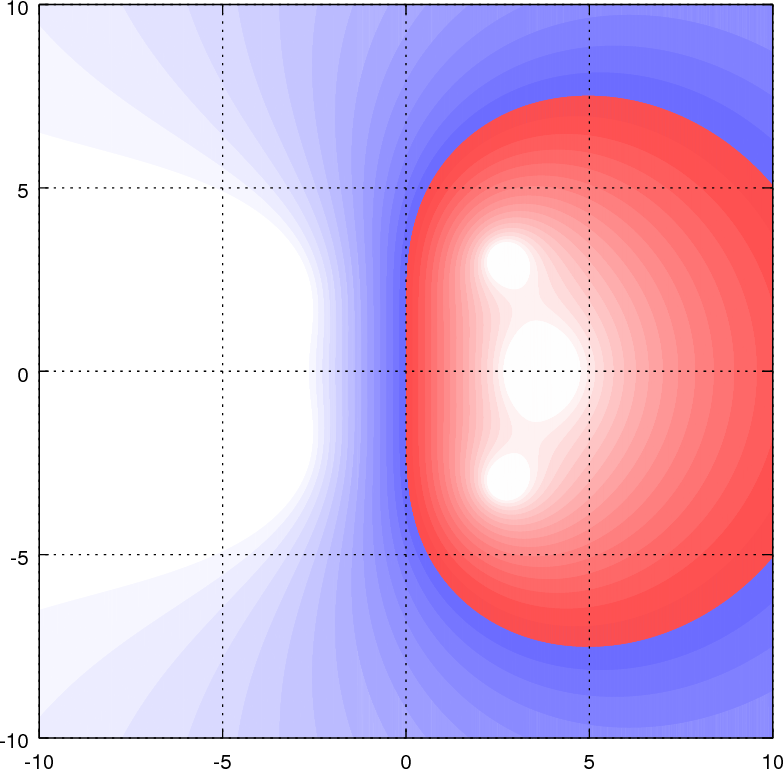
\includegraphics[width=.3\textwidth]{fig/stability-radau3}
  \caption{Stability domains of right Radau-collocation methods with
    one (implicit Euler), two, and three collocation points (left to
    right). Note the different scaling of coordinate axes in
    comparison with previous figures.}
  \label{fig:radau-collocation}
\end{figure}
Observe how not only the stability domains are growing with order of
the method, but also that the computation of $y_1$ coincides with that
of $g_s$, such that we can save a few operations.
\begin{table}[tp]
  \begin{minipage}[t]{.49\linewidth}
    \begin{gather*}
  \def\arraystretch{1.5}
  \begin{array}{c|cc}  
    \frac13 & \frac{5}{12} & -\frac{1}{12}
    \\
    1 & \frac34 & \frac14
    \\\hline
            & \frac34 & \frac14
  \end{array}
\end{gather*}

%%% Local Variables:
%%% mode: latex
%%% TeX-master: "../notes"
%%% End:

  \end{minipage}
  \begin{minipage}[t]{.49\linewidth}
    \begin{gather*}
  \def\arraystretch{1.5}
  \begin{array}{c|ccc}
    \frac{4-\sqrt{6}}{10}
    & \frac{88-7\sqrt6}{360}
    & \frac{296-169\sqrt6}{1800}
    & \frac{-2+3\sqrt{6}}{225}
    \\
    \frac{4+\sqrt{6}}{10}
    & \frac{296+169\sqrt{6}}{1800}
    & \frac{88+7\sqrt{6}}{360}
    & \frac{-2-3\sqrt6}{225}
    \\
    1
    & \frac{16-\sqrt{6}}{36}
    & \frac{16+\sqrt{6}}{36}
    & \frac19
    \\\hline
    & \frac{16-\sqrt{6}}{36}
    & \frac{16+\sqrt{6}}{36}
    & \frac19
  \end{array}  
\end{gather*}

%%% Local Variables:
%%% mode: latex
%%% TeX-master: "../notes"
%%% End:
      
  \end{minipage}
  \caption{Right Radau-collocation methods with two
    and three collocation points}
  \label{tab:radau-collokation-2-3}
\end{table}
\endinput
\section{Considerations on implementation}

\begin{intro}
  Implicit Runge-Kutta methods require the solution of a nonlinear
  system of size $\rks\cdot d$, where $\rks$ is the number of stages
  and $d$ the dimension of the system of ODE. DIRK methods are simpler
  and only require the solution of a system of dimension $d$. Thus, we
  should prefer this class of methods, weren't it for
\end{intro}

\begin{Theorem}{DIRK-order-barrier}
  A B-stable DIRK method has at most order 4
\end{Theorem}

\begin{proof}
  See~\cite[Theorem 13.13]{HairerWanner10}.
\end{proof}

\begin{remark}
  In each step of an IRK, we have to solve a (non-)linear system for
  the quantities $g_i$. First, we note that in order to reduce
  round-off errors, it is advantageous to solve for $z_i = g_i-y_0$,
  since, especially for small time steps, $z_i$ is expected to be much
  smaller than $g_i$. Thus, we have to solve the system
  \begin{gather}
    \label{eq:implicit:21}
    z_i = h \sum_{j=1}^{\rks} a_{ij} f(t_0+c_jh, y_0+z_j),
    \quad
    i=1,\dots,\rks.
  \end{gather}
  Using the Runge-Kutta matrix $A$, we rewrite this as
  \begin{gather}
    \label{eq:implicit:22}
    \begin{pmatrix}
      z_1\\\vdots\\z_\rks
    \end{pmatrix}
    = A
    \begin{pmatrix}
      hf(t_0+c_1h, y_0+z_1)
      \\\vdots\\
      hf(t_0+c_\rks h, y_0+z_\rks)
    \end{pmatrix}.
  \end{gather}
  The latter can be used to avoid additional function evaluations by
  computing
  \begin{gather}
    \label{eq:implicit:23}
    y_1 = y_0 + b^TA^{-1}z, 
  \end{gather}
  which again is numerically much more stable than evaluating $f$ with
  a possibly large Lipschitz constant.
\end{remark}

\begin{remark}
  Each step of the Newton iteration requires the inversion of a 
\end{remark}
%%% Local Variables: 
%%% mode: latex
%%% TeX-master: "notes"
%%% End: 

\chapter{Linear Multistep Methods}


\begin{intro}
  In the previous methods we obtained the value after the next time
  step always by using \emph{one} initial value at the beginning of
  the current time interval, possibly with the
  help of intermediate steps. These methods often are accused to have
  a higher computation time than methods which use several previous
  points, the argument being that function values at these points have
  been computed already. Such methods using values of several time steps in
  the past are called multistep methods. They are constructed such
  that using more steps yields a method of higher order.

  We will begin this chapter by introducing some of the
  formulas. Afterwards, we will study their stability and convergence
  properties.
\end{intro}

\begin{example}[Adams-Moulton formulas]
  \label{ex:lmm:2}  
  \index{Adams-Moulton methods} Basically, there are two construction
  principles for the multistep methods: Quadrature and numerical
  differentiation.  We postpone the latter to example~\ref{ex:lmm:3}
  and deal with the former for now.  As first example we choose the
  class of Adams-Moulton methods for which the integral from point
  $t_{k-1}$ to point $t_{k}$ is approximated by a quadrature of the
  points $t_{k-\lmms}$ to $t_k$, hence
  \begin{gather}
    \label{eq:lmm:16}
    y_k = y_{k-1} + \sum_{r=0}^\lmms f_{k-r} \int_{t_{k-1}}^{t_k}
    L_r(t) \dt,
  \end{gather}
  where $f_j$ denotes the function value $f(t_j, y_j)$ and $L_r(t)$
  the Lagrange interpolation polynomial to point $t_r$ with respect to
  the points $t_{k-\lmms},\dots,t_k$.  This is shown in
  Figure~\ref{fig:lmm:adams-moulton}.
  \begin{figure}[tbp]
    \begin{center}
      \includegraphics[width=.9\textwidth]{fig/adams-moulton.tikz}
    \end{center}
    \caption{The quadrature of Adams-Moulton formulas: the
      integration interval is marked by the wavy line in the end. The support 
			points of the quadrature are stated under the line.}
    \label{fig:lmm:adams-moulton}
  \end{figure}
  Since the integral involves the point being computed itself, these
  methods are implicit. The first of these are
  \begin{align*}
  y_k &= y_{k-1} + h f_k \\
  y_k &= y_{k-1} + \frac12h
        \bigl( f_k + f_{k-1}\bigr)\\
  y_k &= y_{k-1} +
        \frac1{12}h \bigl( 5f_k + 8 f_{k-1} -  f_{k-2}\bigr)\\
  y_k &= y_{k-1} +
        \frac1{24}h \bigl(9f_k+19 f_{k-1}-5 f_{k-2}+ f_{k-3}\bigr)
\end{align*}

%%% Local Variables:
%%% mode: latex
%%% TeX-master: "../notes"
%%% End:
  
\end{example}

\begin{example}[Adams-Bashforth formulas]
  \label{ex:lmm:1}
  \index{Adams-Bashforth methods} With the same principle we obtain
  explicit methods by omitting the point in time $t_k$ in the
  definition of the interpolation polynomial. See
  Figure~\ref{fig:lmm:adams-bashforth}.
  \begin{figure}[tbp]
    \begin{center}
      \includegraphics[width=.9\textwidth]{fig/adams-bashforth.tikz}
    \end{center}
    \caption{The quadrature of Adams-Bashforth formulas: the
      integration interval is marked by the wavy line in the end. The support 
			points of the quadrature are stated under the line.}
    \label{fig:lmm:adams-bashforth}
  \end{figure}
  This yields quadrature formulas of the form
  \begin{gather}
    \label{eq:lmm:17}
    y_k = y_{k-1} + \sum_{r=1}^\lmms f_{k-r} \int_{t_{k-1}}^{t_k}
    L_r(t) \dt.
  \end{gather}
  Again, we list the first few:
  \begin{tikzpicture}
  \draw[snake=snake](7,0) -- (8,0);
  \draw(5,0) -- (7,0);
  % \draw(2,0) -- (3,0);
  \draw[dotted](0,0)--(3,0);
  \draw[dashed](3,0)--(5,0);
  
  \draw(8,-.1) --(8,.1) node[anchor=south]{$t_{k}$};
  \draw(7,-.1) node[anchor=north]{$t_{k-1}$} --(7,.1);
  \draw(6,-.1) node[anchor=north]{$t_{k-2}$} --(6,.1);
  \draw(5,-.1) node[anchor=north]{$t_{k-3}$} --(5,.1);
  
  \draw(3,-.1) node[anchor=north]{$t_{k-\lmms}$} --(3,.1);
  % \draw(2,-.1) --(2,.1) node[anchor=south]{$t_{k-\lmms-1}$};
\end{tikzpicture}

\end{example}

\begin{example}
  \label{ex:lmm:3}
  \index{BDF methods} Backward differencing formulas (BDF) are as well
  based on Lagrange interpolation at the points $t_{k-\lmms}$ to
  $t_k$. In contrast to Adams formulas they do not use quadrature for
  the right hand side, but rather the derivative of the interpolation
  polynomial in the point $t_k$.  Using Lagrange interpolation
  polynomials $L_i(t)$, we let
  \begin{gather*}
    y(t) = \sum_{r=0}^\lmms y_{n-r} L_{n-r}(t),
  \end{gather*}
  where $y_n$ is still to determine. Now we assume that $y$ solves the ODE
  in point $t_n$, hence
  \begin{gather*}
    y'(t_n) = f(t_n, y_n) = \sum_{r=0}^\lmms y_{n-r} L'_{n-r}(t_n).
  \end{gather*}
  This yields the following schemes:
  \begin{align*}
  y_k-y_{k-1} &= h f_k \\
  y_k-\tfrac43 y_{k-1} + \tfrac13y_{k-2} &= \tfrac23 h f_k \\
  y_k-\tfrac{18}{11} y_{k-1} + \tfrac{9}{11} y_{k-2} -
  \tfrac{2}{11} y_{k-3}
              &= \tfrac6{11} h f_k \\
  y_k-\tfrac{48}{25} y_{k-1} + \tfrac{36}{25} y_{k-2} -
  \tfrac{16}{25} y_{k-3} + \tfrac{3}{25} y_{k-4}
              &= \tfrac{12}{25} h f_k
\end{align*}

%%% Local Variables:
%%% mode: latex
%%% TeX-master: "../notes"
%%% End:

  For an example on how to derive these schemes see the appendix.
\end{example}

\begin{remark}
  We know from introduction to numerical analysis, that the numerical
  differentiation and the extrapolation, the evaluation of
  interpolation polynomials outside of the interval which is spanned
  through the interpolation points, are not stable.  Therefore, we
  expect stability problems for the Adams-Bashforth and BDF
  methods. Moreover, we remember that Lagrange interpolation with
  equidistant support points is unstable for a high-degree
  polynomials. Therefore, we also expect that all methods above
  perform well only with moderate order.
\end{remark}

%%%%%%%%%%%%%%%%%%%%%%%%%%%%%%%%%%%%%%%%%%%%%%%%%%%%%%%%%%%%%%%%%%%%%%
%%%%%%%%%%%%%%%%%%%%%%%%%%%%%%%%%%%%%%%%%%%%%%%%%%%%%%%%%%%%%%%%%%%%%%
\section{Definition and consistency of LMM}
%%%%%%%%%%%%%%%%%%%%%%%%%%%%%%%%%%%%%%%%%%%%%%%%%%%%%%%%%%%%%%%%%%%%%%
%%%%%%%%%%%%%%%%%%%%%%%%%%%%%%%%%%%%%%%%%%%%%%%%%%%%%%%%%%%%%%%%%%%%%%

\chapter{Linear Multistep Methods}


\begin{intro}
  In the previous methods we obtained the value after the next time
  step always by using \emph{one} initial value at the beginning of
  the current time interval, possibly with the
  help of intermediate steps. These methods often are accused to have
  a higher computation time than methods which use several previous
  points, the argument being that function values at these points have
  been computed already. Such methods using values of several time steps in
  the past are called multistep methods. They are constructed such
  that using more steps yields a method of higher order.

  We will begin this chapter by introducing some of the
  formulas. Afterwards, we will study their stability and convergence
  properties.
\end{intro}

\begin{example}[Adams-Moulton formulas]
  \label{ex:lmm:2}  
  \index{Adams-Moulton methods} Basically, there are two construction
  principles for the multistep methods: Quadrature and numerical
  differentiation.  We postpone the latter to example~\ref{ex:lmm:3}
  and deal with the former for now.  As first example we choose the
  class of Adams-Moulton methods for which the integral from point
  $t_{k-1}$ to point $t_{k}$ is approximated by a quadrature of the
  points $t_{k-\lmms}$ to $t_k$, hence
  \begin{gather}
    \label{eq:lmm:16}
    y_k = y_{k-1} + \sum_{r=0}^\lmms f_{k-r} \int_{t_{k-1}}^{t_k}
    L_r(t) \dt,
  \end{gather}
  where $f_j$ denotes the function value $f(t_j, y_j)$ and $L_r(t)$
  the Lagrange interpolation polynomial to point $t_r$ with respect to
  the points $t_{k-\lmms},\dots,t_k$.  This is shown in
  Figure~\ref{fig:lmm:adams-moulton}.
  \begin{figure}[tbp]
    \begin{center}
      \includegraphics[width=.9\textwidth]{fig/adams-moulton.tikz}
    \end{center}
    \caption{The quadrature of Adams-Moulton formulas: the
      integration interval is marked by the wavy line in the end. The support 
			points of the quadrature are stated under the line.}
    \label{fig:lmm:adams-moulton}
  \end{figure}
  Since the integral involves the point being computed itself, these
  methods are implicit. The first of these are
  \begin{align*}
  y_k &= y_{k-1} + h f_k \\
  y_k &= y_{k-1} + \frac12h
        \bigl( f_k + f_{k-1}\bigr)\\
  y_k &= y_{k-1} +
        \frac1{12}h \bigl( 5f_k + 8 f_{k-1} -  f_{k-2}\bigr)\\
  y_k &= y_{k-1} +
        \frac1{24}h \bigl(9f_k+19 f_{k-1}-5 f_{k-2}+ f_{k-3}\bigr)
\end{align*}

%%% Local Variables:
%%% mode: latex
%%% TeX-master: "../notes"
%%% End:
  
\end{example}

\begin{example}[Adams-Bashforth formulas]
  \label{ex:lmm:1}
  \index{Adams-Bashforth methods} With the same principle we obtain
  explicit methods by omitting the point in time $t_k$ in the
  definition of the interpolation polynomial. See
  Figure~\ref{fig:lmm:adams-bashforth}.
  \begin{figure}[tbp]
    \begin{center}
      \includegraphics[width=.9\textwidth]{fig/adams-bashforth.tikz}
    \end{center}
    \caption{The quadrature of Adams-Bashforth formulas: the
      integration interval is marked by the wavy line in the end. The support 
			points of the quadrature are stated under the line.}
    \label{fig:lmm:adams-bashforth}
  \end{figure}
  This yields quadrature formulas of the form
  \begin{gather}
    \label{eq:lmm:17}
    y_k = y_{k-1} + \sum_{r=1}^\lmms f_{k-r} \int_{t_{k-1}}^{t_k}
    L_r(t) \dt.
  \end{gather}
  Again, we list the first few:
  \begin{tikzpicture}
  \draw[snake=snake](7,0) -- (8,0);
  \draw(5,0) -- (7,0);
  % \draw(2,0) -- (3,0);
  \draw[dotted](0,0)--(3,0);
  \draw[dashed](3,0)--(5,0);
  
  \draw(8,-.1) --(8,.1) node[anchor=south]{$t_{k}$};
  \draw(7,-.1) node[anchor=north]{$t_{k-1}$} --(7,.1);
  \draw(6,-.1) node[anchor=north]{$t_{k-2}$} --(6,.1);
  \draw(5,-.1) node[anchor=north]{$t_{k-3}$} --(5,.1);
  
  \draw(3,-.1) node[anchor=north]{$t_{k-\lmms}$} --(3,.1);
  % \draw(2,-.1) --(2,.1) node[anchor=south]{$t_{k-\lmms-1}$};
\end{tikzpicture}

\end{example}

\begin{example}
  \label{ex:lmm:3}
  \index{BDF methods} Backward differencing formulas (BDF) are as well
  based on Lagrange interpolation at the points $t_{k-\lmms}$ to
  $t_k$. In contrast to Adams formulas they do not use quadrature for
  the right hand side, but rather the derivative of the interpolation
  polynomial in the point $t_k$.  Using Lagrange interpolation
  polynomials $L_i(t)$, we let
  \begin{gather*}
    y(t) = \sum_{r=0}^\lmms y_{n-r} L_{n-r}(t),
  \end{gather*}
  where $y_n$ is still to determine. Now we assume that $y$ solves the ODE
  in point $t_n$, hence
  \begin{gather*}
    y'(t_n) = f(t_n, y_n) = \sum_{r=0}^\lmms y_{n-r} L'_{n-r}(t_n).
  \end{gather*}
  This yields the following schemes:
  \begin{align*}
  y_k-y_{k-1} &= h f_k \\
  y_k-\tfrac43 y_{k-1} + \tfrac13y_{k-2} &= \tfrac23 h f_k \\
  y_k-\tfrac{18}{11} y_{k-1} + \tfrac{9}{11} y_{k-2} -
  \tfrac{2}{11} y_{k-3}
              &= \tfrac6{11} h f_k \\
  y_k-\tfrac{48}{25} y_{k-1} + \tfrac{36}{25} y_{k-2} -
  \tfrac{16}{25} y_{k-3} + \tfrac{3}{25} y_{k-4}
              &= \tfrac{12}{25} h f_k
\end{align*}

%%% Local Variables:
%%% mode: latex
%%% TeX-master: "../notes"
%%% End:

  For an example on how to derive these schemes see the appendix.
\end{example}

\begin{remark}
  We know from introduction to numerical analysis, that the numerical
  differentiation and the extrapolation, the evaluation of
  interpolation polynomials outside of the interval which is spanned
  through the interpolation points, are not stable.  Therefore, we
  expect stability problems for the Adams-Bashforth and BDF
  methods. Moreover, we remember that Lagrange interpolation with
  equidistant support points is unstable for a high-degree
  polynomials. Therefore, we also expect that all methods above
  perform well only with moderate order.
\end{remark}

%%%%%%%%%%%%%%%%%%%%%%%%%%%%%%%%%%%%%%%%%%%%%%%%%%%%%%%%%%%%%%%%%%%%%%
%%%%%%%%%%%%%%%%%%%%%%%%%%%%%%%%%%%%%%%%%%%%%%%%%%%%%%%%%%%%%%%%%%%%%%
\section{Definition and consistency of LMM}
%%%%%%%%%%%%%%%%%%%%%%%%%%%%%%%%%%%%%%%%%%%%%%%%%%%%%%%%%%%%%%%%%%%%%%
%%%%%%%%%%%%%%%%%%%%%%%%%%%%%%%%%%%%%%%%%%%%%%%%%%%%%%%%%%%%%%%%%%%%%%

\chapter{Linear Multistep Methods}


\begin{intro}
  In the previous methods we obtained the value after the next time
  step always by using \emph{one} initial value at the beginning of
  the current time interval, possibly with the
  help of intermediate steps. These methods often are accused to have
  a higher computation time than methods which use several previous
  points, the argument being that function values at these points have
  been computed already. Such methods using values of several time steps in
  the past are called multistep methods. They are constructed such
  that using more steps yields a method of higher order.

  We will begin this chapter by introducing some of the
  formulas. Afterwards, we will study their stability and convergence
  properties.
\end{intro}

\begin{example}[Adams-Moulton formulas]
  \label{ex:lmm:2}  
  \index{Adams-Moulton methods} Basically, there are two construction
  principles for the multistep methods: Quadrature and numerical
  differentiation.  We postpone the latter to example~\ref{ex:lmm:3}
  and deal with the former for now.  As first example we choose the
  class of Adams-Moulton methods for which the integral from point
  $t_{k-1}$ to point $t_{k}$ is approximated by a quadrature of the
  points $t_{k-\lmms}$ to $t_k$, hence
  \begin{gather}
    \label{eq:lmm:16}
    y_k = y_{k-1} + \sum_{r=0}^\lmms f_{k-r} \int_{t_{k-1}}^{t_k}
    L_r(t) \dt,
  \end{gather}
  where $f_j$ denotes the function value $f(t_j, y_j)$ and $L_r(t)$
  the Lagrange interpolation polynomial to point $t_r$ with respect to
  the points $t_{k-\lmms},\dots,t_k$.  This is shown in
  Figure~\ref{fig:lmm:adams-moulton}.
  \begin{figure}[tbp]
    \begin{center}
      \includegraphics[width=.9\textwidth]{fig/adams-moulton.tikz}
    \end{center}
    \caption{The quadrature of Adams-Moulton formulas: the
      integration interval is marked by the wavy line in the end. The support 
			points of the quadrature are stated under the line.}
    \label{fig:lmm:adams-moulton}
  \end{figure}
  Since the integral involves the point being computed itself, these
  methods are implicit. The first of these are
  \input{definitions/adams-moulton}  
\end{example}

\begin{example}[Adams-Bashforth formulas]
  \label{ex:lmm:1}
  \index{Adams-Bashforth methods} With the same principle we obtain
  explicit methods by omitting the point in time $t_k$ in the
  definition of the interpolation polynomial. See
  Figure~\ref{fig:lmm:adams-bashforth}.
  \begin{figure}[tbp]
    \begin{center}
      \includegraphics[width=.9\textwidth]{fig/adams-bashforth.tikz}
    \end{center}
    \caption{The quadrature of Adams-Bashforth formulas: the
      integration interval is marked by the wavy line in the end. The support 
			points of the quadrature are stated under the line.}
    \label{fig:lmm:adams-bashforth}
  \end{figure}
  This yields quadrature formulas of the form
  \begin{gather}
    \label{eq:lmm:17}
    y_k = y_{k-1} + \sum_{r=1}^\lmms f_{k-r} \int_{t_{k-1}}^{t_k}
    L_r(t) \dt.
  \end{gather}
  Again, we list the first few:
  \input{definitions/adams-bashforth}
\end{example}

\begin{example}
  \label{ex:lmm:3}
  \index{BDF methods} Backward differencing formulas (BDF) are as well
  based on Lagrange interpolation at the points $t_{k-\lmms}$ to
  $t_k$. In contrast to Adams formulas they do not use quadrature for
  the right hand side, but rather the derivative of the interpolation
  polynomial in the point $t_k$.  Using Lagrange interpolation
  polynomials $L_i(t)$, we let
  \begin{gather*}
    y(t) = \sum_{r=0}^\lmms y_{n-r} L_{n-r}(t),
  \end{gather*}
  where $y_n$ is still to determine. Now we assume that $y$ solves the ODE
  in point $t_n$, hence
  \begin{gather*}
    y'(t_n) = f(t_n, y_n) = \sum_{r=0}^\lmms y_{n-r} L'_{n-r}(t_n).
  \end{gather*}
  This yields the following schemes:
  \input{definitions/bdf}
  For an example on how to derive these schemes see the appendix.
\end{example}

\begin{remark}
  We know from introduction to numerical analysis, that the numerical
  differentiation and the extrapolation, the evaluation of
  interpolation polynomials outside of the interval which is spanned
  through the interpolation points, are not stable.  Therefore, we
  expect stability problems for the Adams-Bashforth and BDF
  methods. Moreover, we remember that Lagrange interpolation with
  equidistant support points is unstable for a high-degree
  polynomials. Therefore, we also expect that all methods above
  perform well only with moderate order.
\end{remark}

%%%%%%%%%%%%%%%%%%%%%%%%%%%%%%%%%%%%%%%%%%%%%%%%%%%%%%%%%%%%%%%%%%%%%%
%%%%%%%%%%%%%%%%%%%%%%%%%%%%%%%%%%%%%%%%%%%%%%%%%%%%%%%%%%%%%%%%%%%%%%
\section{Definition and consistency of LMM}
%%%%%%%%%%%%%%%%%%%%%%%%%%%%%%%%%%%%%%%%%%%%%%%%%%%%%%%%%%%%%%%%%%%%%%
%%%%%%%%%%%%%%%%%%%%%%%%%%%%%%%%%%%%%%%%%%%%%%%%%%%%%%%%%%%%%%%%%%%%%%

\input{definitions/lmm}

\begin{remark}
  \index{step size!constant} The LMM was defined for constant step size
  $h$.  In principle it is possible to implement the method with a
  variable step size but we restrict ourselves to the constant case.
  Notes to the step size control can be found later on in this chapter.
\end{remark}

\begin{remark}
  One-step methods were always denoted by describing how to compute
  $y_1$ from $y_0$. Here, the notation becomes more complicated, but
  sometimes we consider only $y_s$ computed from $y_0,\dots,y_{s-1}$
  implying the same rules for $y_k$ computed from
  $y_{k-\lmms},\dots,y_{k-1}$.
\end{remark}
\input{definitions/lmm-errors}

\begin{lemma}
  Consider the differential equation
  \begin{gather*}
    y' = f(t,y) \qquad y(t_0) = y_0
  \end{gather*}
  where f is given continuously differentiable and $y(t)$ is the exact solution.
  For the local error we obtain

  \begin{gather}
    y(t_k)-y_k = \left( \alpha_0 \identity - h\beta_0 \frac{\partial f}{\partial y}(t_k,\eta) \right)^{-1} (L_h u)(t_k).
  \end{gather}

  Here $\eta$ is a value between $y(t_k)$ and $y_k$ if $f$ is a scalar
	function.
  If $f$ is multidimensional, the matrix 
	$\frac{\partial f}{\partial y}(t_k,\eta)$ is the Jacobi matrix, 
	which rows are evaluated at possible places between
	$y(t_k)$ and $y_k$.
\end{lemma}

\begin{proof}
  Considering the local error we can assume exact initial values 
  and therefore we can transform ~\ref{eq:lmm:4} to:
  \begin{gather*}
    \alpha_\lmms y_k + \sum\limits_{r=1}^\lmms \alpha_{\lmms-r} y(t_{k-r})
    = h \left( \beta_\lmms f_k + \sum\limits_{r=1}^\lmms \beta_{\lmms-r} f_{k-r} \right)
  \end{gather*}
  We transform further:
  \begin{multline*}
    \sum\limits_{r=0}^{\lmms} \left( \alpha_r y(t_{k-r})
      - h \beta_r f(t_{k-r},y(t_{k-r})) \right)
    \\
    - \alpha_0 y(t_k) + h \beta_0 f(t_k, y(t_k)) + \alpha_0 y_k
    - h \beta_0 f(t_k,y_k) = 0.
  \end{multline*}
	We now insert ~\ref{eq:lmm:9} which results in
  \begin{gather*}
    (L_h y)(t_k) = \alpha_0 \left( y(t_k) - y_k \right) - h \beta_0 \left( f(t_k,y(t_k)) - f(t_k,y_k) \right)
    \\
    \left( y(t_k) - y_k \right) \left( \alpha_0 \identity - h \beta_0 \frac{f(t_k,y(t_k)) - f(t_k,y_k)}{y(t_k) - y_k} \right)
  \end{gather*}
  By application of the mean value theorem and 
  subsequent transformation we obtain the statement of the theorem.
\end{proof}

      % \cite[Lemma 2.2, p. 369]{HairerNorsettWanner93}

\input{definitions/lmm-consistency}
\input{theorems/lmm-bramble-hilbert}

\begin{proof}
  We start with the Taylor expansion of a solution $u$ of the ODE and
  the corresponding right hand side $f$ for $t_k$, where we insert,
  unlike usual, $f=u'$:
  \begin{alignat*}2
    u(t) &= \sum_{i=0}^p \frac{u^{(i)}(t_k)}{i!}(t-t_k)^i +
    \frac{u^{(p+1)}(\xi)}{(p+1)!}(t-t_k)^{p+1} &=:& \phi(t) + r_u(t)
    \\
    f\bigl(t,u(t)\bigr) &= \sum_{i=1}^p \frac{u^{(i)}(t_k)}{(i-1)!}(t-t_k)^{i-1} +
    \frac{u^{(p+1)}(\xi)}{p!}(t-t_k)^{p} &=:& \phi'(t) + r_f(t),
  \end{alignat*}
  with the Taylor polynomial $\phi(t)$ of degree $p$ and remainder
  $r_u(t)$ and $r_f(t)$. Out of this we calculate:
  \begin{align*}
    L_h u(t_k) =& \sum_{r=0}^\lmms \alpha_{\lmms-r} \phi(t_{k-r}) - h
    \sum_{r=0}^\lmms \beta_{\lmms-r} \phi'(t_{k-r})
    \\
    &+ \sum_{r=0}^\lmms \alpha_{\lmms-r} r_u(t_{k-r}) - h
    \sum_{r=0}^\lmms \beta_{\lmms-r} r_f(t_{k-r}).
  \end{align*}
  Since $t_{k-r}-t_k = r h$, the first row equals a polynomial 
  $\psi(h)$ in $h$ of degree $p$. For the second row we insert the
	reminder estimate $r_u(t) = \mathcal O((t-t_k)^{p+1}) = h
  r_f(t)$ and get:
  \begin{gather}
    \label{eq:lmm:15}
    L_h u(t_k) = L_h \phi(t_k) + \mathcal O(h^{p+1}) = \psi(h) + \mathcal O(h^{p+1}).
  \end{gather}
  According to the definition of the truncation error, this term has to be of
	order $p+1$, such that the method is of order $p$. However it is $\psi$
  of degree $p$. This can only hold true if $L_h\phi=\psi\equiv
  0$. On the other hand $\tau_h(t_k)$ automatically is of order
  $p$. Since $u$ is the solution of an arbitrary right hand side, this
	condition has to be satisfied for all kind of Taylor polynomials $\phi$ 
	of degree $p$.
\end{proof}

\begin{Theorem}{lmm-consistency}
  \index{step size!constant}
  A LMM with constant step size is consistent of order
  $p$ if and only if
    \begin{gather}
      \label{eq:lmm:12}
      \begin{split}
      \sum_{r=0}^\lmms \alpha_{r} &= 0, \\
      \sum_{r=0}^\lmms \bigl(\alpha_{r}r^q - q \beta_{r}
      r^{q-1}\bigr) &= 0,
      \qquad q = 1,\dots,p        
      \end{split}
    \end{gather}
\end{Theorem}


\begin{proof}
  According to lemma~\ref{Lemma:lmm-bramble-hilbert} it is sufficient
  to show that ~\eqref{eq:lmm:12} is equivalent to $L_h \phi_q=0$ for
  polynomials of degree $q\le p$. Due to linearity of the method it
  however is sufficient to show this for a basis of the polynomial
  space of degree $p$.  For that we choose the monomial basis of the
  form
  \begin{gather*}
  \pi_q(t) =
  \left(\frac{t-t_{k-\lmms}}h\right)^q,\qquad q=0,\dots,p.
  \end{gather*}
  For those it holds: $\pi_q(t_{k-r}) = (\lmms-r)^q$. Now we see that
  the first condition is $L_h\pi_0 = 0$ (here is
  $\pi_0'\equiv0$) and the second condition is $L_h\pi_q = 0$.
\end{proof}

\begin{todo}
  Beispiel einer konsistenten LMM, die nicht konvergiert.
\end{todo}

\begin{remark}
  As shown in a homework problem, a consistent LMM is not necessary
  convergent. To understand this behavior and develop criteria for
  convergence we need to diverge into the theory of difference
  equations.
\end{remark}
%%%%%%%%%%%%%%%%%%%%%%%%%%%%%%%%%%%%%%%%%%%%%%%%%%%%%%%%%%%%%%%%%%%%%%
%%%%%%%%%%%%%%%%%%%%%%%%%%%%%%%%%%%%%%%%%%%%%%%%%%%%%%%%%%%%%%%%%%%%%%
\section{Properties of difference equations}
%%%%%%%%%%%%%%%%%%%%%%%%%%%%%%%%%%%%%%%%%%%%%%%%%%%%%%%%%%%%%%%%%%%%%%
%%%%%%%%%%%%%%%%%%%%%%%%%%%%%%%%%%%%%%%%%%%%%%%%%%%%%%%%%%%%%%%%%%%%%%

\begin{intro}
  The stability of LMM can be understood by employing the fairly old
  theory of difference equations. In order to keep the presentation
  simple in this section, we use a different notation for numbering
  indices in the equations. Nevertheless, the coefficients of the
  characteristic polynomial are the same as for LMM.
\end{intro}

\input{definitions/difference-equation}

\begin{Lemma}{lmm:1}
  The solutions of the equation~\eqref{eq:lmm:3} with $y_n\in \R$ or
  $y_n\in \C$ form a vector space of dimension $\lmms$. 
\end{Lemma}

\begin{proof}
  Since the equation~\eqref{eq:lmm:3} is linear and homogeneous, it is
  obvious that if two sequences of solutions $\{y^{(1)}\}$ and
  $\{y^{(2)}\}$ satisfy the equation, sums of multiples of them
  satisfy it too.

  As soon as the initial values $y_0$ to $y_{\lmms-1}$ are chosen, all
  other sequence members are uniquely defined.  Moreover it holds
  \begin{gather*}
    y_0=y_1=\dots=y_{\lmms-1}=0
    \quad\Longrightarrow\quad
    y_n = 0, \;n \ge 0.
  \end{gather*}
  Therefore it is sufficient to consider the first $\lmms$ values.  If
  they are linear independent, then the overall sequences are and vice
  versa. Thus, the initial values form a $\lmms$
  dimensional vector space.
\end{proof}

\input{theorems/difference-equation-solutions}

\begin{proof}
  Inserting the solution $y_n = \xi^n$ into the difference equation
  results in
  \begin{gather*}
    \sum_{r=0}^\lmms \alpha_{r} \xi^{n+r} = \xi^{n}
    \sum_{r=0}^\lmms \alpha_{r} \xi^{r}
    = \xi^{n} \chi(\xi) = 0.
  \end{gather*}
\end{proof}

\input{theorems/difference-equation-basis}

\begin{proof}
  First we observe that the sum of the multiplicities of the roots
  results in the degree of the polynomial:
  \begin{gather*}
    \lmms = \sum_{i=1}^\iota \nu_i.
  \end{gather*}
  Moreover we know because of Lemma~\ref{Lemma:lmm:1}, that $\lmms$ is
  the dimension of the solution space. We show that the sequences
  $\{y^{(i,k)}_n\}$ are linear independent. This is clear for
  sequences of different index $i$. It is also clear for different roots,
  because for $n\to\infty$ the exponential function nullifies the
  influence of the polynomials.
  
  It remains to show that the sequences $\{y^{(i,k)}_n\}$ in fact are
  solutions of the difference equations.  For $k=0$ we have proven
  this already in lemma~\ref{Lemma:difference-equation-solutions}.  We proof the fact here for
  $k=2$ and for a double zero $\xi_i$; the principle for higher order
  roots should be clear then.  Equation~\eqref{eq:lmm:3} applied to
  the sequence $\{n \xi_i^n\}$ results in
  \begin{align*}
    \sum_{r=0}^{\lmms} \alpha_r (n+r) \xi_i^{n+r}
    &= n \xi_i^n \sum_{r=0}^{\lmms} \alpha_r \xi_i^{r}
    + \xi_i^{n+1} \sum_{r=1}^{\lmms} \alpha_r r \xi_i^{r-1}
    \\
    &= n \xi_i^n \rho(\xi_i) + \xi_i^{n+1} \rho'(\xi_i) = 0.
  \end{align*}
  Here the term with $\alpha_0$ vanishes, because it is multiplied
  with $r=0$. $\rho(\xi_i) = \rho'(\xi_i) = 0$ because $\xi_i$ is a
  multiple root.
\end{proof}

\input{theorems/root-test}

\begin{proof}
  According to theorem~\ref{Theorem:difference-equation-basis} we can write all solutions
  as linear combinations of the sequences $y^{(i,k)}$ in
  equation~\eqref{eq:lmm:6}. Therefore,
  \begin{enumerate}
  \item all solutions to $|\xi_i|<1$ for $n\to\infty$ converge to zero
  \item all solutions to $|\xi_i|>1$ for $n\to\infty$ divergence to infinity
  \item all solutions to $|\xi_i|=1$ for $n\to\infty$ stay bounded 
	if and only if $\xi_i$ is simple.
  \end{enumerate}
  This proves the statement of the theorem.
\end{proof}

%%%%%%%%%%%%%%%%%%%%%%%%%%%%%%%%%%%%%%%%%%%%%%%%%%%%%%%%%%%%%%%%%%%%%%
%%%%%%%%%%%%%%%%%%%%%%%%%%%%%%%%%%%%%%%%%%%%%%%%%%%%%%%%%%%%%%%%%%%%%%
\section{Stability and convergence}
%%%%%%%%%%%%%%%%%%%%%%%%%%%%%%%%%%%%%%%%%%%%%%%%%%%%%%%%%%%%%%%%%%%%%%
%%%%%%%%%%%%%%%%%%%%%%%%%%%%%%%%%%%%%%%%%%%%%%%%%%%%%%%%%%%%%%%%%%%%%%

\begin{remark}
  In contrast to one-step methods the convergence of multistep methods
  follows not directly from the consistency of the method, if the
  right hand side of the differential equation satisfies the Lipschitz
  condition~\eqref{eq:IVP:1}.  Analog to the A-stability we will
  discuss this by means of a simple model problem and we will deduce
  stability conditions.
\end{remark}

\begin{remark}
  In the following we investigate the solution to a fixed point in time
  $t$ with a shrinking step size $h$. Therefore we choose $n$
  steps of step size $h = t/n$ and let $n$ go towards infinity.
\end{remark}

\input{definitions/lmm-stability}
\input{theorems/lmm-stability}

\begin{proof}
  The application of the LMM to the equation~\eqref{eq:lmm:1} results
  in the difference equation
  \begin{gather*}
    \sum_{r=0}^{\lmms} \alpha_{\lmms-r} y_{n-r} = 0.
  \end{gather*}
  Now we have to proof that the solutions for fixed $t = h n$ stay
  bounded if $h\to 0$. But we also see that the upper equation does
  not contain $h$. Therefore we have to examine, if the solutions
  $y_n$ stay bounded for $n\to \infty$.  By resorting the summation we
  obtain a difference equation of the form~\eqref{eq:lmm:3}. Due to
  corollary~\ref{Corollary:root-test} it follows the statement of the theorem.
\end{proof}

\begin{Corollary}{adams-stability}
  Adams-Bashforth and Adams-Moulton methods are stable.
\end{Corollary}

\begin{proof}
  For all of these methods the first generating polynomial is $\rho(x)
  = x^\lmms-x^{\lmms-1}$. It has the simple root $\xi_1 = 1$ and the
  $\lmms-1$-fold root 0.
\end{proof}

\begin{Theorem}{BDF-stability}
  The BDF methods are stable for $\lmms \le 6$ and not
  stable for $\lmms \ge 7$.
\end{Theorem}

\input{definitions/lmm-convergence}
\input{theorems/lmm-one-step}

\begin{proof}
  From the general form of LMM we
  obtain
  \begin{gather*}
    \frac1{\alpha_s} \sum_{r=0}^\lmms \alpha_{\lmms-r} y_{k-r}
    = \frac{h}{\alpha_s} \sum_{r=0}^{\lmms-1} \beta_{\lmms-r} f_{k-r}
    + \beta_s f_k.
  \end{gather*}
  We rewrite this to
  \begin{gather*}
    y_k = -\sum_{r=1}^{\lmms} \alpha'_{\lmms-r} y_{k-r} +
    h\psi_h(t_{k-1}, Y_{k-1}),
  \end{gather*}
  where we implicitly enter this formula as value for $y_k$ in the
  computation of $f_k$. It remains to realize that this is the first
  set of $d$ equations in~\eqref{eq:lmm-one-step:1}, and that the
  remaining ones are just shifting $y_i$ to $y_{i+1}$.
\end{proof}

\input{theorems/lmm-one-consistency}

\begin{proof}
  The first component of $Y_k - \widehat Y_k$ is the local error of
  step $k$, which is of order $h^{p+1}$ by the assumption. The other
  components vanish by the definition of the method.
\end{proof}

\input{theorems/lmm-one-stability}

\begin{proof}
  We notice that $\widehat\rho(x) = \sum \alpha'_{s-r} x^r$ is the
  characteristic polynomial of the matrix $A$ and thus its eigenvalues
  are the roots of $\widehat\rho(x)$, which has the same roots as the
  generating polynomial $\rho(x)$. By the root test, we know that
  simple roots, which correspond to irreducible blocks of dimension
  one have maximal modulus one. Furthermore, every Jordan block of
  dimension greater than one corresponds to a multiple root, which by
  assumption has modulus strictly less than one. It is easy to see
  that such a block admits a modified canonical form
  \begin{gather*}
    J_i =
    \begin{pmatrix}
      \lambda_i & 1- \abs{\lambda_i}\\
        & \lambda_i &\ddots\\
          &&\ddots & 1- \abs{\lambda_i}\\
            &&&\lambda_i
    \end{pmatrix}.
  \end{gather*}
  Thus, the canonical form $J = T^{-1}AT$ has norm $\norm{J}_{\infty}
  \le 1$. If we define the norm
  \begin{gather*}
    \norm{x} = \norm{(T^{-1}\otimes \identity)x}_\infty,
  \end{gather*}
  we obtain the result by
  \begin{multline*}
    \norm{(A\otimes \identity)x}
    = \norm{(T^{-1}\otimes \identity)(A\otimes \identity)x}_\infty
    = \norm{(J\otimes \identity)(T^{-1}\otimes \identity)x}_\infty
    \\
    \le \norm{(T^{-1}\otimes \identity)x}_\infty
    = \norm{x}.
  \end{multline*}
\end{proof}

\input{theorems/lmm-convergence}

\begin{proof}
  We reduce the proof to convergence of a one-step method with
  \begin{gather}
    \label{eq:lmm:18}
    Y_k = G(Y_{k-1}) =  (A\otimes \identity) Y_{k-1} + h \verfahren_h(t_{k-1}, Y_{k-1}).
  \end{gather}
  Let $Y_{k-1}$ and $Z_{k-1}$ be two initial values for the interval $I_k$.
  By the previous lemma, we have in the norm defined there, for
  sufficiently small $h$, and assuming a Lipschitz constant $L_h$ for
  $\verfahren_h$ :
  \begin{gather}
    \label{eq:lmm:19}
    \norm{G(Y_{k-1})-G(Z_{k-1})} \le (1+h L_h) \norm{Y_{k-1}-Z_{k-1}}.
  \end{gather}
  Thus, the local error $\eta_k = U_k - \widehat Y_k$ at step $k$, which by
  Lemma~\ref{Lemma:lmm-one-consistency} is bounded by $M h^{p+1}$, accumulates
  until step $n$ at most to $h^{p+1}(1_h L_h)^{n-k}$.

  We have:
  \begin{align*}
    \norm{U_1 - Y_1} &\le (1+h L_h)\norm{U_0-y_0} + M h^{p+1} \\
    \norm{U_2 - Y_2} &\le (1+h L_h)^2\norm{U_0-y_0} +  M h^{p+1} \bigl(1+ (1+h L_h)\bigr)\\
    \norm{U_3 - Y_3} &\le (1+h L_h)^3\norm{U_0-y_0} +  M h^{p+1} \Bigl(\bigl(1+ (1+h L_h)+ (1+h L_h)^2\bigr)\Bigr)\\
    \norm{U_n-Y_n} &\le e^{n h L_h}\norm{U_0-Y_0} +
    \frac{M h^p}{L_h}\bigl(e^{n h L_h} - 1\bigr).
  \end{align*}
\end{proof}

\subsection{Starting procedures}

\begin{intro}
In contrast to one-step methods, where the numerical solution is obtained 
solely from the differential equation and the initial value, multistep 
methods require more than one start value. An LMM with $s$ steps requires $s$ 
known start values $y_{k-s}, \dots, y_{k-1}$. Mostly, they are not provided 
by the IVP itself. Thus, general LMM decompose into two parts: 
\begin{itemize}
\item a \emph{starting phase} where the start values are computed in a 
suitable way and
\item a \emph{run phase} where the LMM is executed. 
\end{itemize}
It is crucial that the method of the starting phase provides a suitable order 
corresponding to the LMM of the run phase, recall Definition 
\ref{Definition:lmm-convergence}. Moreover, it should have analog properties to 
the LMM, like explicit/implicit or applicability to stiff problems. 
% We now consider different starting procedures for an implicit LMM with 
% convergence order $p$. According to Definition \ref{Definition:lmm-convergence} 
% the starting values are required to have the same convergence order. 
Possible choices for the starting phase include multistep methods with variable 
order and one-step methods.  
\end{intro}

\begin{example}[Self starter]
A 2-step BDF method requires $y_0$ and $y_1$ to be known. $y_0$ is given by the 
initial value while $y_1$ is unknown so far. To guarantee that the method has 
order 2, $y_1$ needs to be locally of order 2 at least
\begin{align}\label{eq:lmm_1BDFstarter}
|u(t_1)-y_1| \leq c_0 h^2.
\end{align}
This is ensured, for example, by one step of the 1-step BDF method.

However, starting an LMM with $s>2$ steps by a first-order method and then 
successively increasing the order until $s$ is reached does not provide the 
desired global order. That is due to the fact that the first step limits  
the overall convergence order to 2, compare \eqref{eq:lmm_1BDFstarter}. 
Nevertheless, self starters are often used in practice. 
\end{example}
% In this case local 
% error estimates are used to bound the errors of the starting values and all 
% approximations of the run phase by reducing the step sizes, 
% %. Moreover, also in 
% %the run phase the step sizes are controlled using local error estimates, 
% see the  
% discussion on step size control in Section \ref{section:step_size_control}. 


\begin{example}[Runge-Kutta starter]
\label{Example:RKstarter}
One can use Runge-Kutta methods to start LMM. Since only a fixed
number of starting steps are performed, the local order of the
Runge-Kutta approximation is crucial.  For an implicit LMM with
convergence order $p$ and stepsize $h$ one could use an RK method with
consistency order $p-1$ with the same stepsize $h$.

Consider a 3-step BDF method. Thus, beside $y_0$, we need start values 
$y_1, y_2$ with errors less than $c_0 h^3$. They can be computed by RK methods 
of consistency order $2$, for example by two steps of the 1-stage Gau\ss \ 
collocation method with step size $h$ since it has consistency order $2s=2$, 
see theorem \ref{Theorem:gauss-consistency}.
\end{example}




\begin{example}[Continuous Runge-Kutta starter]
  Another option is to use continuous Runge-Kutta methods and to
  evaluate the continuous approximation to obtain the required
  starting values.

  In constrast to Example \ref{Example:RKstarter} one could also use
  the continuous polynomial approximation of Gau\ss \ collocation to
  start a 3-step BDF method. One step with step size $2h$ of a 2-stage
  Gau\ss \ collocation method would give a polynomial of degree $2$
  which is then evaluated in $t_1=t_0+h$ and $t_2=t_1+h$ to obtain
  $y_1, y_2$. According to Theorem
  \ref{Theorem:collocation-continuous} $y_1, y_2$ have the appropriate
  order.
\end{example}

\begin{remark}
  In practice not the order of a procedure is crucial but rather the
  fact that the errors of all approximations (the start values and all
  approximations of the run phase) are bounded by the user-given
  tolerance, compare Section \ref{section:step_size_control}. Thus,
  the step sizes of all steps are controlled using local error
  estimates. Hence, self starting procedures usually start with very
  small step sizes and increase them successively. Due to their higher
  orders RK starters usually are allowed to use moderate step sizes in
  the beginning. Generally, LMM are applied with variable step sizes
  and orders in practice (see e.g. Exercise 7.2).
\end{remark}



%%%%%%%%%%%%%%%%%%%%%%%%%%%%%%%%%%%%%%%%%%%%%%%%%%%%%%%%%%%%%%%%%%%%%%
%%%%%%%%%%%%%%%%%%%%%%%%%%%%%%%%%%%%%%%%%%%%%%%%%%%%%%%%%%%%%%%%%%%%%%
\section{LMM and stiff problems}
%%%%%%%%%%%%%%%%%%%%%%%%%%%%%%%%%%%%%%%%%%%%%%%%%%%%%%%%%%%%%%%%%%%%%%
%%%%%%%%%%%%%%%%%%%%%%%%%%%%%%%%%%%%%%%%%%%%%%%%%%%%%%%%%%%%%%%%%%%%%%

\begin{Definition*}{lmm-stability-region}{A-stability of LMM}
  \index{stability region!of a LMM}
  The linear model difference equation
  \begin{gather}
    \label{eq:lmm:7}
    \sum_{r=0}^{\lmms} \bigl(\alpha_{\lmms-r} - z \beta_{\lmms-r}) y_{n-r} = 0.
  \end{gather}
  is obtained by applying an LMM to the model equation
  $u' = \lambda u$ and inserting $z=h\lambda$.

  The \define{stability region} of an LMM is the set of points $z\in \C$,
  for which all solution sequences $\{y_n\}$ of the equation~\eqref{eq:lmm:7}
  stay bounded for $n\to\infty$. An LMM is called \define{A-stable}, if the 
  stability region contains the left half-plane of $\C$.
\end{Definition*}


\begin{Definition}{lmm-stability-polynomial}
  The stability polynomial of an LMM is obtained by inserting
  $y_n = x^n$ into the linear model difference equation to obtain
  \begin{gather}
    \label{eq:lmm:8}
    r_z(x) = \sum_{r=0}^{\lmms} \bigl(\alpha_{\lmms-r} - z \beta_{\lmms-r})
    x^{\lmms-r}.
  \end{gather}
\end{Definition}

\begin{remark}
  Instead of the simple amplification function $r(z)$ of the one-step
  methods, we get here a function of two variables.  The point $z$ for
  which we want to show stability and the artificial variable $x$ from
  the analysis of the method.
\end{remark}

\begin{Lemma}{lmm-stability}
  Let $\{\xi_1(z),\dots,\xi_\lmms(z)\}$ be the set of roots of the
  stability polynomial $r_z(x)$ as functions of $z$.
  A point $z\in \C$ is in the stability region of a LMM, if these
  roots satisfy the root test in corollary~\ref{Corollary:root-test}.
\end{Lemma}

\begin{proof}
  The proof is analog to theorem~\ref{Theorem:lmm-stability}.
\end{proof}

\begin{Theorem*}{dahlquist2}{2nd Dahlquist barrier}
  \defindex{Dahlquist barrier (second)} There is no A-stable LMM of
  order $p>2$. Among the A-stable LMM of order 2, the trapezoidal rule
  (Crank-Nicolson) has the smallest error constant.
\end{Theorem*}

\subsection{Relaxed A-stability}

\begin{intro}
  Motivated by the fact that there are no higher order A-stable LMM
  and by highly dissipative problems, people have introduced relaxed
  concepts of A-stability.
\end{intro}

\input{definitions/aa-stability}

\begin{remark}
  The introduction of the A(0)-stability is motivated by linear
  systems of the form $u'=-Au$ with symmetric, positive definite
  matrix $A$. In fact one requires there only stability on the real
  axis because all eigenvalues are real. Thus, any positive angle
  $\alpha$ is sufficient.
  
  Similarly A($\alpha$)-stable LMM are suitable for linear problems in
  which high frequently vibration ($\Im\lambda$ large) decay fast
  ($-\Re\lambda$ large).

  In all cases one observes corresponding properties of the Jacobian
  matrix $\partial_u f$ for the application of nonlinear problems.
\end{remark}

\begin{example}
  The stability regions of the stable BDF methods are in
  Figure~\ref{fig:bdf-stability}. The corresponding values for
  A($\alpha$)-stability and stiff stability are in Table  
\ref{tab:bdf-stability}.
\end{example}
\begin{figure}[tp]
  \centering
  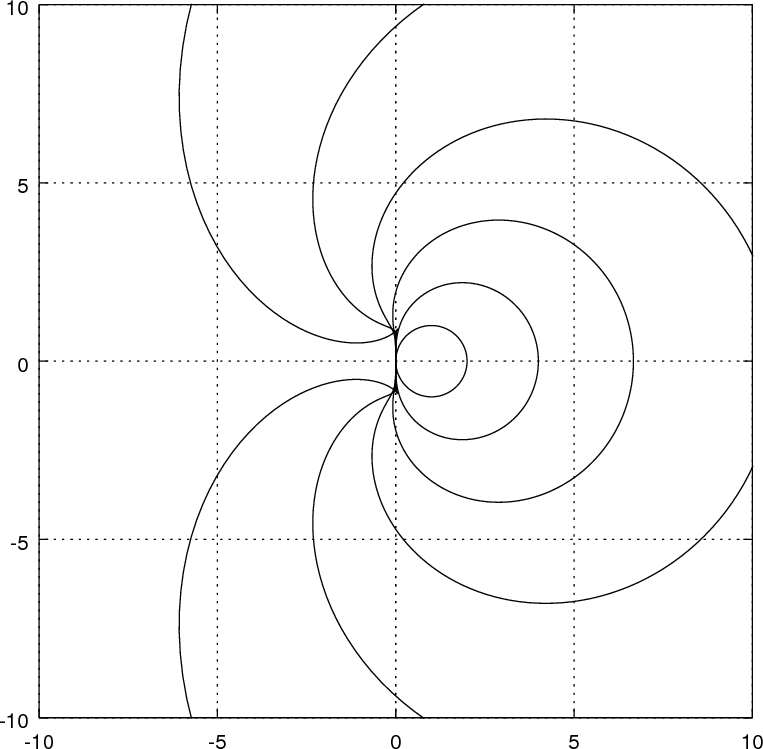
\includegraphics[width=.45\textwidth]{fig/stability-bdf.png}
  \hfill
  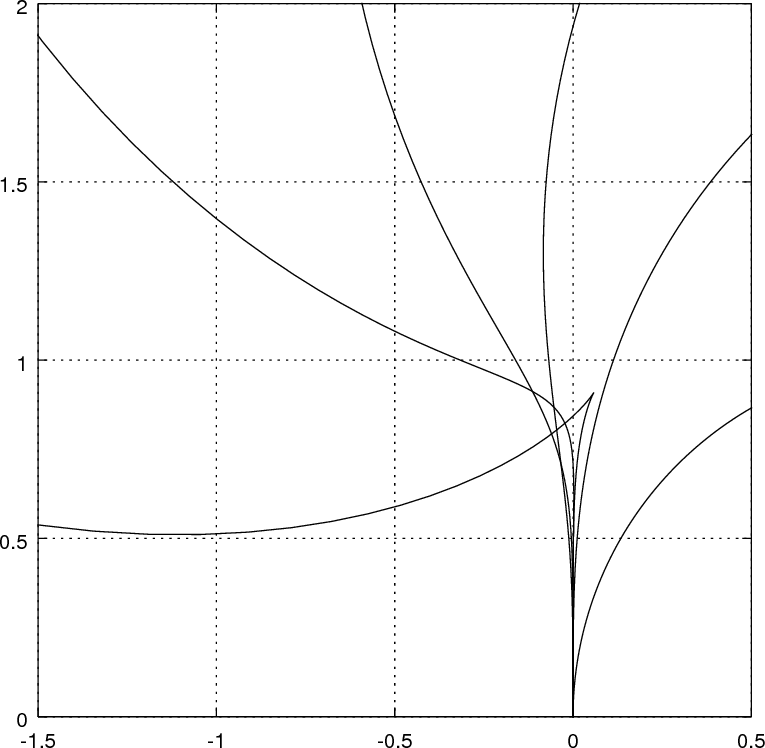
\includegraphics[width=.45\textwidth]{fig/stability-bdf-zoom.png}
  \caption{Boundaries of stability regions of BDF1 to BDF6. Unstable
    region right of the origin. Zoom on the right}
  \label{fig:bdf-stability}
\end{figure}
\begin{table}[tp]
  \centering
  \begin{tabular}{c|cccccc}
    $k$ & 1 & 2 & 3 & 4 & 5 & 6 \\\hline
    $\alpha$ & 90$^\circ$ & 90$^\circ$& 86.03$^\circ$
                    & 73.35$^\circ$& 51.84$^\circ$
                            & 17.84$^\circ$ \\
    $D$ & 0 & 0 & 0.083& 0.667& 2.327& 6.075
  \end{tabular}
  \caption{Values for A($\alpha$)- and stiff stability for BDF methods
    of order $k$.}
  \label{tab:bdf-stability}
\end{table}

%%%%%%%%%%%%%%%%%%%%%%%%%%%%%%%%%%%%%%%%%%%%%%%%%%%%%%%%%%%%%%%%%%%%%%
\section{Predictor-corrector schemes}

\begin{Definition*}{predictor-corrector}{Predictor-corrector methods}
  Assume a pair of time stepping schemes, one explicit, one implicit,
  \begin{align*}
    \hat y_{k} &= \hat \verfahren_p(y_{k-1}) \\
    y_k &= \verfahren_c(y_{k-1},y_{k}),
  \end{align*}
  we can use $\hat y_k$ as initial value for the Newton iteration for
  $y_k$. In an extreme case, we let
  \begin{gather*}
    y_k = \verfahren_c(y_{k-1},\hat y_{k}),
  \end{gather*}
  without any further iteration.
\end{Definition*}

\begin{remark}
  Predictor-corrector methods were developed strongly around
  Adams-Moulton and Adams-Bashforth methods, since the implicit ones
  have much smaller error constants. Given that these methods offer no
  considerable advantages compared to Runge-Kutta methods, but
  stability properties and implementation are weak points, We omit
  their discussion.

  A simple predictor for BDF methods can be obtained, since they are
  based on an interpolating polynomial. Thus, we simply extrapolate
  this polynomial to the next point in time.
\end{remark}

\begin{example}
  While the predictor-corrector idea sounds reasonable, we have to be
  careful with stiff problems, the original reason for using implicit
  methods. Take again our favorite IVP
  \begin{gather*}
    u' = \lambda u,
    \qquad u(0) = 1.
  \end{gather*}
  We apply the BDF(1) scheme, namely the implicit Euler method, with
  step size 1. According to its stability
  function~\eqref{eq:impl:stabil:impleuler}, we obtain
  \begin{gather*}
    y_1 = \frac1{1-\lambda}.
  \end{gather*}
  Hence, the interpolating polynomial is
  \begin{gather*}
    y(t) = (1-t) + \frac1{1-\lambda} t = 1 + \frac{\lambda}{1-\lambda}t.
  \end{gather*}
  For the mildly stiff problem $\lambda = -3$, we obtain
  \begin{gather*}
    y_1 = 0.25, \qquad y_2 = 0.0625,
    \qquad \hat y_2 = y(2) = -0.5.
  \end{gather*}
  Thus, the extrapolated value is already a much worse initial value
  for a Newton iteration than using the value from the previous time
  step.
  
  While this example was particularly chosen to exhibit such failure,
  it does show that extrapolation of stiff problems has its
  pitfalls. Here, we end up with a time step restriction which is
  comparable to the stability condition of the explicit method.
\end{example}


%%% Local Variables: 
%%% mode: latex
%%% TeX-master: "notes"
%%% End: 


\begin{remark}
  \index{step size!constant} The LMM was defined for constant step size
  $h$.  In principle it is possible to implement the method with a
  variable step size but we restrict ourselves to the constant case.
  Notes to the step size control can be found later on in this chapter.
\end{remark}

\begin{remark}
  One-step methods were always denoted by describing how to compute
  $y_1$ from $y_0$. Here, the notation becomes more complicated, but
  sometimes we consider only $y_s$ computed from $y_0,\dots,y_{s-1}$
  implying the same rules for $y_k$ computed from
  $y_{k-\lmms},\dots,y_{k-1}$.
\end{remark}
\begin{Definition}{lmm-errors}
    \index{Lh@$L_h$|textbf}
  We express the LMM with the linear \define{difference operator}
  \begin{gather}
    \label{eq:lmm:9}
    (L_hu)(t_k) = \sum_{r=0}^{\lmms}\Bigl(\alpha_{\lmms-r} u(t_{k-r}) - h
    \beta_{R-r} f\bigl(t_{k-r},u(t_{k-r})\bigr)\Bigr)
  \end{gather}
  and for a continuous function $u$ we define the \textbf{truncation
    error}\defindex{truncation error!LMM}
  \begin{gather}
    \label{eq:lmm:10}
    \tau_h(t_k) = \tfrac1hL_hu(t_k).
  \end{gather}
  The \textbf{local error} \defindex{LMM!local error}\defindex{local
    error!LMM} of a linear multistep method is defined by
  \begin{gather*}
    u(t_\lmms) - y_\lmms
  \end{gather*}
  where $u(t)$ denotes the exact solution of $u' = f(t,u), u(t_0)=u_0$
  and $y_s$ the numerical solution by using the exact initial values
 	$y_i = u(t_i)$ for $i = 0,1,...,s-1$.
\end{Definition}

%%% Local Variables:
%%% mode: latex
%%% TeX-master: "../notes"
%%% End:


\begin{lemma}
  Consider the differential equation
  \begin{gather*}
    y' = f(t,y) \qquad y(t_0) = y_0
  \end{gather*}
  where f is given continuously differentiable and $y(t)$ is the exact solution.
  For the local error we obtain

  \begin{gather}
    y(t_k)-y_k = \left( \alpha_0 \identity - h\beta_0 \frac{\partial f}{\partial y}(t_k,\eta) \right)^{-1} (L_h u)(t_k).
  \end{gather}

  Here $\eta$ is a value between $y(t_k)$ and $y_k$ if $f$ is a scalar
	function.
  If $f$ is multidimensional, the matrix 
	$\frac{\partial f}{\partial y}(t_k,\eta)$ is the Jacobi matrix, 
	which rows are evaluated at possible places between
	$y(t_k)$ and $y_k$.
\end{lemma}

\begin{proof}
  Considering the local error we can assume exact initial values 
  and therefore we can transform ~\ref{eq:lmm:4} to:
  \begin{gather*}
    \alpha_\lmms y_k + \sum\limits_{r=1}^\lmms \alpha_{\lmms-r} y(t_{k-r})
    = h \left( \beta_\lmms f_k + \sum\limits_{r=1}^\lmms \beta_{\lmms-r} f_{k-r} \right)
  \end{gather*}
  We transform further:
  \begin{multline*}
    \sum\limits_{r=0}^{\lmms} \left( \alpha_r y(t_{k-r})
      - h \beta_r f(t_{k-r},y(t_{k-r})) \right)
    \\
    - \alpha_0 y(t_k) + h \beta_0 f(t_k, y(t_k)) + \alpha_0 y_k
    - h \beta_0 f(t_k,y_k) = 0.
  \end{multline*}
	We now insert ~\ref{eq:lmm:9} which results in
  \begin{gather*}
    (L_h y)(t_k) = \alpha_0 \left( y(t_k) - y_k \right) - h \beta_0 \left( f(t_k,y(t_k)) - f(t_k,y_k) \right)
    \\
    \left( y(t_k) - y_k \right) \left( \alpha_0 \identity - h \beta_0 \frac{f(t_k,y(t_k)) - f(t_k,y_k)}{y(t_k) - y_k} \right)
  \end{gather*}
  By application of the mean value theorem and 
  subsequent transformation we obtain the statement of the theorem.
\end{proof}

      % \cite[Lemma 2.2, p. 369]{HairerNorsettWanner93}

\begin{Definition}{lmm-consistency}
  An LMM is consistent of order $p$, if for all sufficient regular
  functions $u$ and all relevant $k$ there holds
  \begin{gather}
    \label{eq:lmm:11}
    \tau_h(t_k) = \mathcal O(h^p),
  \end{gather}
  or equivalently, that the \putindex{local error} is $\mathcal O(h^{p+1})$.
\end{Definition}

%%% Local Variables:
%%% mode: latex
%%% TeX-master: "../notes"
%%% End:

\begin{Lemma}{lmm-bramble-hilbert}
  An LMM is consistent of order $p$ if and only if for all polynomials
  $\phi_q$ of degree $q \le p$ and $f(t,q(t)) = q'(t)$ there holds:
  \begin{gather}
    \label{eq:lmm:14}
    L_h \phi_q = 0.
  \end{gather}
\end{Lemma}

%%% Local Variables:
%%% mode: latex
%%% TeX-master: "../notes"
%%% End:


\begin{proof}
  We start with the Taylor expansion of a solution $u$ of the ODE and
  the corresponding right hand side $f$ for $t_k$, where we insert,
  unlike usual, $f=u'$:
  \begin{alignat*}2
    u(t) &= \sum_{i=0}^p \frac{u^{(i)}(t_k)}{i!}(t-t_k)^i +
    \frac{u^{(p+1)}(\xi)}{(p+1)!}(t-t_k)^{p+1} &=:& \phi(t) + r_u(t)
    \\
    f\bigl(t,u(t)\bigr) &= \sum_{i=1}^p \frac{u^{(i)}(t_k)}{(i-1)!}(t-t_k)^{i-1} +
    \frac{u^{(p+1)}(\xi)}{p!}(t-t_k)^{p} &=:& \phi'(t) + r_f(t),
  \end{alignat*}
  with the Taylor polynomial $\phi(t)$ of degree $p$ and remainder
  $r_u(t)$ and $r_f(t)$. Out of this we calculate:
  \begin{align*}
    L_h u(t_k) =& \sum_{r=0}^\lmms \alpha_{\lmms-r} \phi(t_{k-r}) - h
    \sum_{r=0}^\lmms \beta_{\lmms-r} \phi'(t_{k-r})
    \\
    &+ \sum_{r=0}^\lmms \alpha_{\lmms-r} r_u(t_{k-r}) - h
    \sum_{r=0}^\lmms \beta_{\lmms-r} r_f(t_{k-r}).
  \end{align*}
  Since $t_{k-r}-t_k = r h$, the first row equals a polynomial 
  $\psi(h)$ in $h$ of degree $p$. For the second row we insert the
	reminder estimate $r_u(t) = \mathcal O((t-t_k)^{p+1}) = h
  r_f(t)$ and get:
  \begin{gather}
    \label{eq:lmm:15}
    L_h u(t_k) = L_h \phi(t_k) + \mathcal O(h^{p+1}) = \psi(h) + \mathcal O(h^{p+1}).
  \end{gather}
  According to the definition of the truncation error, this term has to be of
	order $p+1$, such that the method is of order $p$. However it is $\psi$
  of degree $p$. This can only hold true if $L_h\phi=\psi\equiv
  0$. On the other hand $\tau_h(t_k)$ automatically is of order
  $p$. Since $u$ is the solution of an arbitrary right hand side, this
	condition has to be satisfied for all kind of Taylor polynomials $\phi$ 
	of degree $p$.
\end{proof}

\begin{Theorem}{lmm-consistency}
  \index{step size!constant}
  A LMM with constant step size is consistent of order
  $p$ if and only if
    \begin{gather}
      \label{eq:lmm:12}
      \begin{split}
      \sum_{r=0}^\lmms \alpha_{r} &= 0, \\
      \sum_{r=0}^\lmms \bigl(\alpha_{r}r^q - q \beta_{r}
      r^{q-1}\bigr) &= 0,
      \qquad q = 1,\dots,p        
      \end{split}
    \end{gather}
\end{Theorem}


\begin{proof}
  According to lemma~\ref{Lemma:lmm-bramble-hilbert} it is sufficient
  to show that ~\eqref{eq:lmm:12} is equivalent to $L_h \phi_q=0$ for
  polynomials of degree $q\le p$. Due to linearity of the method it
  however is sufficient to show this for a basis of the polynomial
  space of degree $p$.  For that we choose the monomial basis of the
  form
  \begin{gather*}
  \pi_q(t) =
  \left(\frac{t-t_{k-\lmms}}h\right)^q,\qquad q=0,\dots,p.
  \end{gather*}
  For those it holds: $\pi_q(t_{k-r}) = (\lmms-r)^q$. Now we see that
  the first condition is $L_h\pi_0 = 0$ (here is
  $\pi_0'\equiv0$) and the second condition is $L_h\pi_q = 0$.
\end{proof}

\begin{todo}
  Beispiel einer konsistenten LMM, die nicht konvergiert.
\end{todo}

\begin{remark}
  As shown in a homework problem, a consistent LMM is not necessary
  convergent. To understand this behavior and develop criteria for
  convergence we need to diverge into the theory of difference
  equations.
\end{remark}
%%%%%%%%%%%%%%%%%%%%%%%%%%%%%%%%%%%%%%%%%%%%%%%%%%%%%%%%%%%%%%%%%%%%%%
%%%%%%%%%%%%%%%%%%%%%%%%%%%%%%%%%%%%%%%%%%%%%%%%%%%%%%%%%%%%%%%%%%%%%%
\section{Properties of difference equations}
%%%%%%%%%%%%%%%%%%%%%%%%%%%%%%%%%%%%%%%%%%%%%%%%%%%%%%%%%%%%%%%%%%%%%%
%%%%%%%%%%%%%%%%%%%%%%%%%%%%%%%%%%%%%%%%%%%%%%%%%%%%%%%%%%%%%%%%%%%%%%

\begin{intro}
  The stability of LMM can be understood by employing the fairly old
  theory of difference equations. In order to keep the presentation
  simple in this section, we use a different notation for numbering
  indices in the equations. Nevertheless, the coefficients of the
  characteristic polynomial are the same as for LMM.
\end{intro}

\begin{Definition}{difference-equation}
  An equation of the form
  \begin{gather}
    \label{eq:lmm:3}
    \sum_{r=0}^\lmms \alpha_{r} y_{n+r} = 0
  \end{gather}
  is called a homogeneous \define{difference equation}. A sequence
  $\{y_n\}_{n=0,\dots,\infty}$ is solution of the difference equation,
  if the equation holds true for all $n\ge \lmms$. The values
  $y_n$ may be from any of the spaces $\R$, $\C$, $\R^d$ or $\C^d$.

  The \define{generating polynomial} of this difference equation
  is
  \begin{gather}
    \label{eq:lmm:2}
    \chi(x) = \sum_{r=0}^\lmms \alpha_{r} x^{r}.
  \end{gather}

\end{Definition}

%%% Local Variables:
%%% mode: latex
%%% TeX-master: "../notes"
%%% End:


\begin{Lemma}{lmm:1}
  The solutions of the equation~\eqref{eq:lmm:3} with $y_n\in \R$ or
  $y_n\in \C$ form a vector space of dimension $\lmms$. 
\end{Lemma}

\begin{proof}
  Since the equation~\eqref{eq:lmm:3} is linear and homogeneous, it is
  obvious that if two sequences of solutions $\{y^{(1)}\}$ and
  $\{y^{(2)}\}$ satisfy the equation, sums of multiples of them
  satisfy it too.

  As soon as the initial values $y_0$ to $y_{\lmms-1}$ are chosen, all
  other sequence members are uniquely defined.  Moreover it holds
  \begin{gather*}
    y_0=y_1=\dots=y_{\lmms-1}=0
    \quad\Longrightarrow\quad
    y_n = 0, \;n \ge 0.
  \end{gather*}
  Therefore it is sufficient to consider the first $\lmms$ values.  If
  they are linear independent, then the overall sequences are and vice
  versa. Thus, the initial values form a $\lmms$
  dimensional vector space.
\end{proof}

\begin{Lemma}{difference-equation-solutions}
  For each root $\xi$ of the generating polynomial $\chi(x)$ the
  sequence $y_n = \xi^n$ is a solution of the difference
  equation~\eqref{eq:lmm:3}.
\end{Lemma}


%%% Local Variables: 
%%% mode: latex
%%% TeX-master: "../notes"
%%% End: 


\begin{proof}
  Inserting the solution $y_n = \xi^n$ into the difference equation
  results in
  \begin{gather*}
    \sum_{r=0}^\lmms \alpha_{r} \xi^{n+r} = \xi^{n}
    \sum_{r=0}^\lmms \alpha_{r} \xi^{r}
    = \xi^{n} \chi(\xi) = 0.
  \end{gather*}
\end{proof}

\begin{Theorem}{difference-equation-basis}
  Let $\{\xi_i\}_{i=1,\dots,\iota}$ be the roots of the
  generating polynomial $\chi$ with multiplicity $\nu_i$. Then,
  the sequences of the form
  \begin{gather}
    \label{eq:lmm:6}
%    y^{(i,k)}_n = p_k(n)\xi_i^n
    y^{(i,k)}_n = n^{k-1}\xi_i^n
    \quad i=1,\dots,\iota; \quad k = 1,\dots,\nu_i
  \end{gather}
%  mit den Polynomen
%  \begin{gather*}
%    p_0(n) = 1 \quad p_k(n) = \prod_{\kappa=0}^{k-1} (n-\kappa)
%  \end{gather*}
  form a basis of the solution space of the difference
  equation~\eqref{eq:lmm:3}.
\end{Theorem}


%%% Local Variables: 
%%% mode: latex
%%% TeX-master: "../notes"
%%% End: 


\begin{proof}
  First we observe that the sum of the multiplicities of the roots
  results in the degree of the polynomial:
  \begin{gather*}
    \lmms = \sum_{i=1}^\iota \nu_i.
  \end{gather*}
  Moreover we know because of Lemma~\ref{Lemma:lmm:1}, that $\lmms$ is
  the dimension of the solution space. We show that the sequences
  $\{y^{(i,k)}_n\}$ are linear independent. This is clear for
  sequences of different index $i$. It is also clear for different roots,
  because for $n\to\infty$ the exponential function nullifies the
  influence of the polynomials.
  
  It remains to show that the sequences $\{y^{(i,k)}_n\}$ in fact are
  solutions of the difference equations.  For $k=0$ we have proven
  this already in lemma~\ref{Lemma:difference-equation-solutions}.  We proof the fact here for
  $k=2$ and for a double zero $\xi_i$; the principle for higher order
  roots should be clear then.  Equation~\eqref{eq:lmm:3} applied to
  the sequence $\{n \xi_i^n\}$ results in
  \begin{align*}
    \sum_{r=0}^{\lmms} \alpha_r (n+r) \xi_i^{n+r}
    &= n \xi_i^n \sum_{r=0}^{\lmms} \alpha_r \xi_i^{r}
    + \xi_i^{n+1} \sum_{r=1}^{\lmms} \alpha_r r \xi_i^{r-1}
    \\
    &= n \xi_i^n \rho(\xi_i) + \xi_i^{n+1} \rho'(\xi_i) = 0.
  \end{align*}
  Here the term with $\alpha_0$ vanishes, because it is multiplied
  with $r=0$. $\rho(\xi_i) = \rho'(\xi_i) = 0$ because $\xi_i$ is a
  multiple root.
\end{proof}

\begin{Corollary*}{root-test}{Root test}
  All solutions $\{y_n\}$ of the difference equation~\eqref{eq:lmm:3}
  are bounded for $n\to\infty$ if and only if it holds:
  \begin{itemize}
  \item all roots of the generating polynomial $\chi(x)$
    lie in the closed unit circle $\bigl\{z\in \C \big|\; |z|\le
    1\bigr\}$ and
  \item all roots on the boundary of the unit circle are simple.
  \end{itemize}
\end{Corollary*}

%%% Local Variables: 
%%% mode: latex
%%% TeX-master: "../notes"
%%% End: 


\begin{proof}
  According to theorem~\ref{Theorem:difference-equation-basis} we can write all solutions
  as linear combinations of the sequences $y^{(i,k)}$ in
  equation~\eqref{eq:lmm:6}. Therefore,
  \begin{enumerate}
  \item all solutions to $|\xi_i|<1$ for $n\to\infty$ converge to zero
  \item all solutions to $|\xi_i|>1$ for $n\to\infty$ divergence to infinity
  \item all solutions to $|\xi_i|=1$ for $n\to\infty$ stay bounded 
	if and only if $\xi_i$ is simple.
  \end{enumerate}
  This proves the statement of the theorem.
\end{proof}

%%%%%%%%%%%%%%%%%%%%%%%%%%%%%%%%%%%%%%%%%%%%%%%%%%%%%%%%%%%%%%%%%%%%%%
%%%%%%%%%%%%%%%%%%%%%%%%%%%%%%%%%%%%%%%%%%%%%%%%%%%%%%%%%%%%%%%%%%%%%%
\section{Stability and convergence}
%%%%%%%%%%%%%%%%%%%%%%%%%%%%%%%%%%%%%%%%%%%%%%%%%%%%%%%%%%%%%%%%%%%%%%
%%%%%%%%%%%%%%%%%%%%%%%%%%%%%%%%%%%%%%%%%%%%%%%%%%%%%%%%%%%%%%%%%%%%%%

\begin{remark}
  In contrast to one-step methods the convergence of multistep methods
  follows not directly from the consistency of the method, if the
  right hand side of the differential equation satisfies the Lipschitz
  condition~\eqref{eq:IVP:1}.  Analog to the A-stability we will
  discuss this by means of a simple model problem and we will deduce
  stability conditions.
\end{remark}

\begin{remark}
  In the following we investigate the solution to a fixed point in time
  $t$ with a shrinking step size $h$. Therefore we choose $n$
  steps of step size $h = t/n$ and let $n$ go towards infinity.
\end{remark}

\begin{Theorem}{lmm-stability}
  A LMM is stable if and only if all roots of the first
  generating polynomial $\rho(x)$ of equation~\eqref{eq:lmm:5} lie
  in the unit circle of the complex plane and all roots on the
  boundary of the unit circle are simple.
\end{Theorem}


%%% Local Variables: 
%%% mode: latex
%%% TeX-master: "../notes"
%%% End: 

\begin{Theorem}{lmm-stability}
  A LMM is stable if and only if all roots of the first
  generating polynomial $\rho(x)$ of equation~\eqref{eq:lmm:5} lie
  in the unit circle of the complex plane and all roots on the
  boundary of the unit circle are simple.
\end{Theorem}


%%% Local Variables: 
%%% mode: latex
%%% TeX-master: "../notes"
%%% End: 


\begin{proof}
  The application of the LMM to the equation~\eqref{eq:lmm:1} results
  in the difference equation
  \begin{gather*}
    \sum_{r=0}^{\lmms} \alpha_{\lmms-r} y_{n-r} = 0.
  \end{gather*}
  Now we have to proof that the solutions for fixed $t = h n$ stay
  bounded if $h\to 0$. But we also see that the upper equation does
  not contain $h$. Therefore we have to examine, if the solutions
  $y_n$ stay bounded for $n\to \infty$.  By resorting the summation we
  obtain a difference equation of the form~\eqref{eq:lmm:3}. Due to
  corollary~\ref{Corollary:root-test} it follows the statement of the theorem.
\end{proof}

\begin{Corollary}{adams-stability}
  Adams-Bashforth and Adams-Moulton methods are stable.
\end{Corollary}

\begin{proof}
  For all of these methods the first generating polynomial is $\rho(x)
  = x^\lmms-x^{\lmms-1}$. It has the simple root $\xi_1 = 1$ and the
  $\lmms-1$-fold root 0.
\end{proof}

\begin{Theorem}{BDF-stability}
  The BDF methods are stable for $\lmms \le 6$ and not
  stable for $\lmms \ge 7$.
\end{Theorem}

\begin{Theorem}{lmm-convergence}
  If a linear multi-step method is stable and consistent of order $p$,
  then it is convergent of order $p$.
\end{Theorem}

%%% Local Variables: 
%%% mode: latex
%%% TeX-master: "../notes"
%%% End: 

\begin{Lemma}{lmm-one-step}
  Every multistep method can be recast as a one-step method
  \begin{gather}
    \label{eq:lmm-one-step:1}
    Y_{k} = (A \otimes \identity) Y_{k-1} + h \verfahren_h(t_{k-1}, Y_{k-1})
  \end{gather}
  where with $\alpha_r' = \alpha_r/\alpha_s$
  \begin{gather}
    \label{eq:lmm-one-step:2}
    Y_k =
    \begin{pmatrix}
      y_k \\ \vdots \\ y_{k-s+1}
    \end{pmatrix},
    \quad
    A =
    \begin{pmatrix}
      -\alpha_{\lmms-1}' & -\alpha_{\lmms-2}' & \cdots & -\alpha_{0}'\\
      1 & 0 & \cdots & 0 \\
      & \ddots & \cdots & 0 \\
      & & 1 & 0
    \end{pmatrix},
  \end{gather}
  and $\verfahren_h(t_k, Y_k) = (e_1 \otimes \identity) \psi_h(t_{k-1}, Y_{k-1})$ with
  $\beta_r' = \beta_r/\alpha_s$ and $\psi_h$ defined implicitly by
  \begin{multline}
    \label{eq:lmm-one-step:3}
    \psi_h(t_{k-1}, Y_{k-1})
    =\sum_{r=1}^{\lmms} \beta_{\lmms-r} f(t_{k-r},y_{k-r})
    \\
    + \beta_s' f\left(t_k, h\psi_h(t_{k-1}, Y_{k-1}) -
      \sum_{r=1}^{\lmms} \alpha_{\lmms-r}' y_{k-r}\right).
  \end{multline}
\end{Lemma}

%%% Local Variables: 
%%% mode: latex
%%% TeX-master: "../notes"
%%% End: 


\begin{proof}
  From the general form of LMM we
  obtain
  \begin{gather*}
    \frac1{\alpha_s} \sum_{r=0}^\lmms \alpha_{\lmms-r} y_{k-r}
    = \frac{h}{\alpha_s} \sum_{r=0}^{\lmms-1} \beta_{\lmms-r} f_{k-r}
    + \beta_s f_k.
  \end{gather*}
  We rewrite this to
  \begin{gather*}
    y_k = -\sum_{r=1}^{\lmms} \alpha'_{\lmms-r} y_{k-r} +
    h\psi_h(t_{k-1}, Y_{k-1}),
  \end{gather*}
  where we implicitly enter this formula as value for $y_k$ in the
  computation of $f_k$. It remains to realize that this is the first
  set of $d$ equations in~\eqref{eq:lmm-one-step:1}, and that the
  remaining ones are just shifting $y_i$ to $y_{i+1}$.
\end{proof}

\begin{Lemma}{lmm-one-consistency}
  Let $u(t)$ be the exact solution of the IVP. For $k=s,\ldots$, we
  define the vector $\widehat Y_{k}$ as the solution of a single step
  \begin{gather*}
    \widehat Y_{k} = (A\otimes I) U_{k-1} + h \verfahren_h(t_{k-1} U_{k-1}),
  \end{gather*}
  with correct initial values $U_{k-1} =
  (u_{k-1},u_{k-2},\dots,u_{k-\lmms})^T$.
  
  If the multistep method is consistent of order $p$, and $f$ is
  sufficiently smooth, then there exist constants $h_0>0$  and $M$
  such that for $h\le h_0$ there holds
  \begin{gather}
    \label{eq:lmm-one-consistency:1}
    \norm{Y_k-\widehat Y_h} \le M h^{p+1}.
  \end{gather}
\end{Lemma}

%%% Local Variables: 
%%% mode: latex
%%% TeX-master: "../notes"
%%% End: 


\begin{proof}
  The first component of $Y_k - \widehat Y_k$ is the local error of
  step $k$, which is of order $h^{p+1}$ by the assumption. The other
  components vanish by the definition of the method.
\end{proof}

\begin{Lemma}{lmm-one-stability}
  Assume that an LMM is stable. Then, there exists a vector norm on
  $\C^{\lmms d}$ such that the operator norm of the matrix $A$
  satisfies
  \begin{gather}
    \label{eq:lmm-one-stability:1}
    \norm{A\otimes \identity} \le 1.
  \end{gather}
\end{Lemma}

%%% Local Variables: 
%%% mode: latex
%%% TeX-master: "../notes"
%%% End: 


\begin{proof}
  We notice that $\widehat\rho(x) = \sum \alpha'_{s-r} x^r$ is the
  characteristic polynomial of the matrix $A$ and thus its eigenvalues
  are the roots of $\widehat\rho(x)$, which has the same roots as the
  generating polynomial $\rho(x)$. By the root test, we know that
  simple roots, which correspond to irreducible blocks of dimension
  one have maximal modulus one. Furthermore, every Jordan block of
  dimension greater than one corresponds to a multiple root, which by
  assumption has modulus strictly less than one. It is easy to see
  that such a block admits a modified canonical form
  \begin{gather*}
    J_i =
    \begin{pmatrix}
      \lambda_i & 1- \abs{\lambda_i}\\
        & \lambda_i &\ddots\\
          &&\ddots & 1- \abs{\lambda_i}\\
            &&&\lambda_i
    \end{pmatrix}.
  \end{gather*}
  Thus, the canonical form $J = T^{-1}AT$ has norm $\norm{J}_{\infty}
  \le 1$. If we define the norm
  \begin{gather*}
    \norm{x} = \norm{(T^{-1}\otimes \identity)x}_\infty,
  \end{gather*}
  we obtain the result by
  \begin{multline*}
    \norm{(A\otimes \identity)x}
    = \norm{(T^{-1}\otimes \identity)(A\otimes \identity)x}_\infty
    = \norm{(J\otimes \identity)(T^{-1}\otimes \identity)x}_\infty
    \\
    \le \norm{(T^{-1}\otimes \identity)x}_\infty
    = \norm{x}.
  \end{multline*}
\end{proof}

\begin{Theorem}{lmm-convergence}
  If a linear multi-step method is stable and consistent of order $p$,
  then it is convergent of order $p$.
\end{Theorem}

%%% Local Variables: 
%%% mode: latex
%%% TeX-master: "../notes"
%%% End: 


\begin{proof}
  We reduce the proof to convergence of a one-step method with
  \begin{gather}
    \label{eq:lmm:18}
    Y_k = G(Y_{k-1}) =  (A\otimes \identity) Y_{k-1} + h \verfahren_h(t_{k-1}, Y_{k-1}).
  \end{gather}
  Let $Y_{k-1}$ and $Z_{k-1}$ be two initial values for the interval $I_k$.
  By the previous lemma, we have in the norm defined there, for
  sufficiently small $h$, and assuming a Lipschitz constant $L_h$ for
  $\verfahren_h$ :
  \begin{gather}
    \label{eq:lmm:19}
    \norm{G(Y_{k-1})-G(Z_{k-1})} \le (1+h L_h) \norm{Y_{k-1}-Z_{k-1}}.
  \end{gather}
  Thus, the local error $\eta_k = U_k - \widehat Y_k$ at step $k$, which by
  Lemma~\ref{Lemma:lmm-one-consistency} is bounded by $M h^{p+1}$, accumulates
  until step $n$ at most to $h^{p+1}(1_h L_h)^{n-k}$.

  We have:
  \begin{align*}
    \norm{U_1 - Y_1} &\le (1+h L_h)\norm{U_0-y_0} + M h^{p+1} \\
    \norm{U_2 - Y_2} &\le (1+h L_h)^2\norm{U_0-y_0} +  M h^{p+1} \bigl(1+ (1+h L_h)\bigr)\\
    \norm{U_3 - Y_3} &\le (1+h L_h)^3\norm{U_0-y_0} +  M h^{p+1} \Bigl(\bigl(1+ (1+h L_h)+ (1+h L_h)^2\bigr)\Bigr)\\
    \norm{U_n-Y_n} &\le e^{n h L_h}\norm{U_0-Y_0} +
    \frac{M h^p}{L_h}\bigl(e^{n h L_h} - 1\bigr).
  \end{align*}
\end{proof}

\subsection{Starting procedures}

\begin{intro}
In contrast to one-step methods, where the numerical solution is obtained 
solely from the differential equation and the initial value, multistep 
methods require more than one start value. An LMM with $s$ steps requires $s$ 
known start values $y_{k-s}, \dots, y_{k-1}$. Mostly, they are not provided 
by the IVP itself. Thus, general LMM decompose into two parts: 
\begin{itemize}
\item a \emph{starting phase} where the start values are computed in a 
suitable way and
\item a \emph{run phase} where the LMM is executed. 
\end{itemize}
It is crucial that the method of the starting phase provides a suitable order 
corresponding to the LMM of the run phase, recall Definition 
\ref{Definition:lmm-convergence}. Moreover, it should have analog properties to 
the LMM, like explicit/implicit or applicability to stiff problems. 
% We now consider different starting procedures for an implicit LMM with 
% convergence order $p$. According to Definition \ref{Definition:lmm-convergence} 
% the starting values are required to have the same convergence order. 
Possible choices for the starting phase include multistep methods with variable 
order and one-step methods.  
\end{intro}

\begin{example}[Self starter]
A 2-step BDF method requires $y_0$ and $y_1$ to be known. $y_0$ is given by the 
initial value while $y_1$ is unknown so far. To guarantee that the method has 
order 2, $y_1$ needs to be locally of order 2 at least
\begin{align}\label{eq:lmm_1BDFstarter}
|u(t_1)-y_1| \leq c_0 h^2.
\end{align}
This is ensured, for example, by one step of the 1-step BDF method.

However, starting an LMM with $s>2$ steps by a first-order method and then 
successively increasing the order until $s$ is reached does not provide the 
desired global order. That is due to the fact that the first step limits  
the overall convergence order to 2, compare \eqref{eq:lmm_1BDFstarter}. 
Nevertheless, self starters are often used in practice. 
\end{example}
% In this case local 
% error estimates are used to bound the errors of the starting values and all 
% approximations of the run phase by reducing the step sizes, 
% %. Moreover, also in 
% %the run phase the step sizes are controlled using local error estimates, 
% see the  
% discussion on step size control in Section \ref{section:step_size_control}. 


\begin{example}[Runge-Kutta starter]
\label{Example:RKstarter}
One can use Runge-Kutta methods to start LMM. Since only a fixed
number of starting steps are performed, the local order of the
Runge-Kutta approximation is crucial.  For an implicit LMM with
convergence order $p$ and stepsize $h$ one could use an RK method with
consistency order $p-1$ with the same stepsize $h$.

Consider a 3-step BDF method. Thus, beside $y_0$, we need start values 
$y_1, y_2$ with errors less than $c_0 h^3$. They can be computed by RK methods 
of consistency order $2$, for example by two steps of the 1-stage Gau\ss \ 
collocation method with step size $h$ since it has consistency order $2s=2$, 
see theorem \ref{Theorem:gauss-consistency}.
\end{example}




\begin{example}[Continuous Runge-Kutta starter]
  Another option is to use continuous Runge-Kutta methods and to
  evaluate the continuous approximation to obtain the required
  starting values.

  In constrast to Example \ref{Example:RKstarter} one could also use
  the continuous polynomial approximation of Gau\ss \ collocation to
  start a 3-step BDF method. One step with step size $2h$ of a 2-stage
  Gau\ss \ collocation method would give a polynomial of degree $2$
  which is then evaluated in $t_1=t_0+h$ and $t_2=t_1+h$ to obtain
  $y_1, y_2$. According to Theorem
  \ref{Theorem:collocation-continuous} $y_1, y_2$ have the appropriate
  order.
\end{example}

\begin{remark}
  In practice not the order of a procedure is crucial but rather the
  fact that the errors of all approximations (the start values and all
  approximations of the run phase) are bounded by the user-given
  tolerance, compare Section \ref{section:step_size_control}. Thus,
  the step sizes of all steps are controlled using local error
  estimates. Hence, self starting procedures usually start with very
  small step sizes and increase them successively. Due to their higher
  orders RK starters usually are allowed to use moderate step sizes in
  the beginning. Generally, LMM are applied with variable step sizes
  and orders in practice (see e.g. Exercise 7.2).
\end{remark}



%%%%%%%%%%%%%%%%%%%%%%%%%%%%%%%%%%%%%%%%%%%%%%%%%%%%%%%%%%%%%%%%%%%%%%
%%%%%%%%%%%%%%%%%%%%%%%%%%%%%%%%%%%%%%%%%%%%%%%%%%%%%%%%%%%%%%%%%%%%%%
\section{LMM and stiff problems}
%%%%%%%%%%%%%%%%%%%%%%%%%%%%%%%%%%%%%%%%%%%%%%%%%%%%%%%%%%%%%%%%%%%%%%
%%%%%%%%%%%%%%%%%%%%%%%%%%%%%%%%%%%%%%%%%%%%%%%%%%%%%%%%%%%%%%%%%%%%%%

\begin{Definition*}{lmm-stability-region}{A-stability of LMM}
  \index{stability region!of a LMM}
  The linear model difference equation
  \begin{gather}
    \label{eq:lmm:7}
    \sum_{r=0}^{\lmms} \bigl(\alpha_{\lmms-r} - z \beta_{\lmms-r}) y_{n-r} = 0.
  \end{gather}
  is obtained by applying an LMM to the model equation
  $u' = \lambda u$ and inserting $z=h\lambda$.

  The \define{stability region} of an LMM is the set of points $z\in \C$,
  for which all solution sequences $\{y_n\}$ of the equation~\eqref{eq:lmm:7}
  stay bounded for $n\to\infty$. An LMM is called \define{A-stable}, if the 
  stability region contains the left half-plane of $\C$.
\end{Definition*}


\begin{Definition}{lmm-stability-polynomial}
  The stability polynomial of an LMM is obtained by inserting
  $y_n = x^n$ into the linear model difference equation to obtain
  \begin{gather}
    \label{eq:lmm:8}
    r_z(x) = \sum_{r=0}^{\lmms} \bigl(\alpha_{\lmms-r} - z \beta_{\lmms-r})
    x^{\lmms-r}.
  \end{gather}
\end{Definition}

\begin{remark}
  Instead of the simple amplification function $r(z)$ of the one-step
  methods, we get here a function of two variables.  The point $z$ for
  which we want to show stability and the artificial variable $x$ from
  the analysis of the method.
\end{remark}

\begin{Lemma}{lmm-stability}
  Let $\{\xi_1(z),\dots,\xi_\lmms(z)\}$ be the set of roots of the
  stability polynomial $r_z(x)$ as functions of $z$.
  A point $z\in \C$ is in the stability region of a LMM, if these
  roots satisfy the root test in corollary~\ref{Corollary:root-test}.
\end{Lemma}

\begin{proof}
  The proof is analog to theorem~\ref{Theorem:lmm-stability}.
\end{proof}

\begin{Theorem*}{dahlquist2}{2nd Dahlquist barrier}
  \defindex{Dahlquist barrier (second)} There is no A-stable LMM of
  order $p>2$. Among the A-stable LMM of order 2, the trapezoidal rule
  (Crank-Nicolson) has the smallest error constant.
\end{Theorem*}

\subsection{Relaxed A-stability}

\begin{intro}
  Motivated by the fact that there are no higher order A-stable LMM
  and by highly dissipative problems, people have introduced relaxed
  concepts of A-stability.
\end{intro}

\begin{Definition}{aa-stability}
  \defindex{A($\alpha$)-stable}
  A set is called \textbf{A($\alpha$)-stable}, if its stability region
  contains the sector
  \begin{gather*}
    \bigg\{z\in \C\;\bigg|\; \Re z < 0 \;\wedge\; \left|\frac{\Im
        z}{\Re z}\right| \le \tan \alpha\biggr\}.
  \end{gather*}
  It is called \textbf{A(0)-stable}, if the negative real axis is contained in
  the stability region.

  It is called \define{stiffly stable}, if it contains the set
  $\{\Re(z)< -D\}$.
\end{Definition}

%%% Local Variables:
%%% mode: latex
%%% TeX-master: "../notes"
%%% End:


\begin{remark}
  The introduction of the A(0)-stability is motivated by linear
  systems of the form $u'=-Au$ with symmetric, positive definite
  matrix $A$. In fact one requires there only stability on the real
  axis because all eigenvalues are real. Thus, any positive angle
  $\alpha$ is sufficient.
  
  Similarly A($\alpha$)-stable LMM are suitable for linear problems in
  which high frequently vibration ($\Im\lambda$ large) decay fast
  ($-\Re\lambda$ large).

  In all cases one observes corresponding properties of the Jacobian
  matrix $\partial_u f$ for the application of nonlinear problems.
\end{remark}

\begin{example}
  The stability regions of the stable BDF methods are in
  Figure~\ref{fig:bdf-stability}. The corresponding values for
  A($\alpha$)-stability and stiff stability are in Table  
\ref{tab:bdf-stability}.
\end{example}
\begin{figure}[tp]
  \centering
  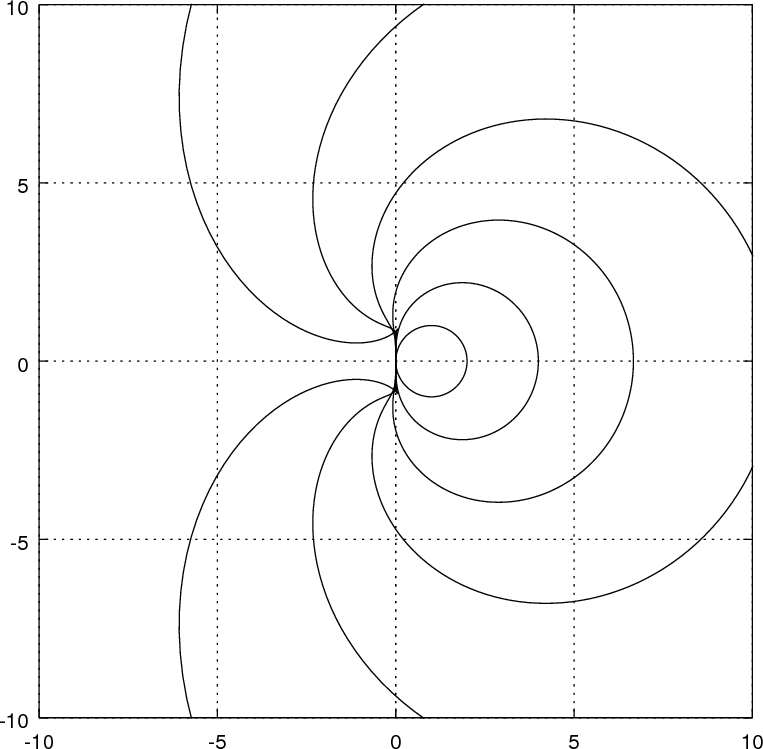
\includegraphics[width=.45\textwidth]{fig/stability-bdf.png}
  \hfill
  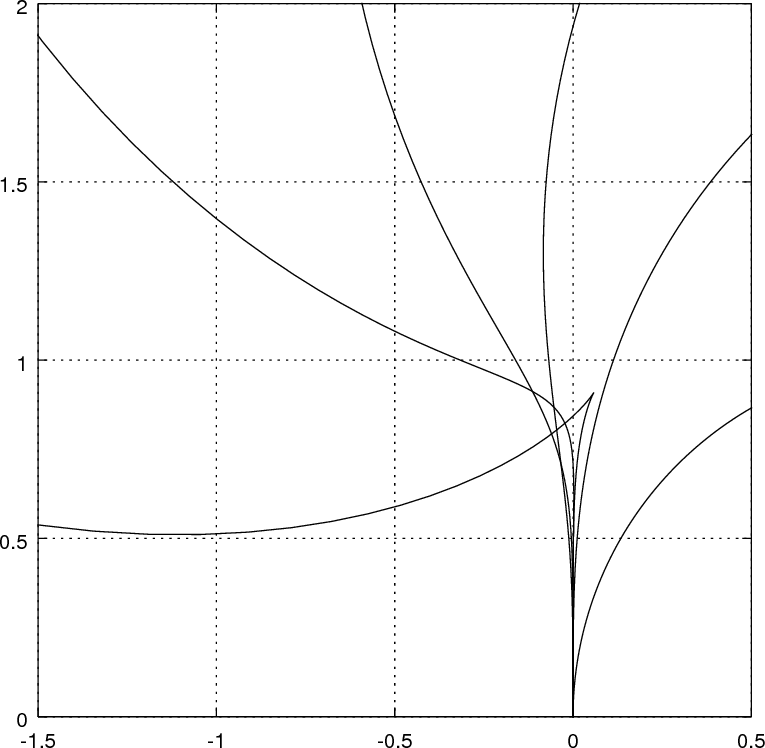
\includegraphics[width=.45\textwidth]{fig/stability-bdf-zoom.png}
  \caption{Boundaries of stability regions of BDF1 to BDF6. Unstable
    region right of the origin. Zoom on the right}
  \label{fig:bdf-stability}
\end{figure}
\begin{table}[tp]
  \centering
  \begin{tabular}{c|cccccc}
    $k$ & 1 & 2 & 3 & 4 & 5 & 6 \\\hline
    $\alpha$ & 90$^\circ$ & 90$^\circ$& 86.03$^\circ$
                    & 73.35$^\circ$& 51.84$^\circ$
                            & 17.84$^\circ$ \\
    $D$ & 0 & 0 & 0.083& 0.667& 2.327& 6.075
  \end{tabular}
  \caption{Values for A($\alpha$)- and stiff stability for BDF methods
    of order $k$.}
  \label{tab:bdf-stability}
\end{table}

%%%%%%%%%%%%%%%%%%%%%%%%%%%%%%%%%%%%%%%%%%%%%%%%%%%%%%%%%%%%%%%%%%%%%%
\section{Predictor-corrector schemes}

\begin{Definition*}{predictor-corrector}{Predictor-corrector methods}
  Assume a pair of time stepping schemes, one explicit, one implicit,
  \begin{align*}
    \hat y_{k} &= \hat \verfahren_p(y_{k-1}) \\
    y_k &= \verfahren_c(y_{k-1},y_{k}),
  \end{align*}
  we can use $\hat y_k$ as initial value for the Newton iteration for
  $y_k$. In an extreme case, we let
  \begin{gather*}
    y_k = \verfahren_c(y_{k-1},\hat y_{k}),
  \end{gather*}
  without any further iteration.
\end{Definition*}

\begin{remark}
  Predictor-corrector methods were developed strongly around
  Adams-Moulton and Adams-Bashforth methods, since the implicit ones
  have much smaller error constants. Given that these methods offer no
  considerable advantages compared to Runge-Kutta methods, but
  stability properties and implementation are weak points, We omit
  their discussion.

  A simple predictor for BDF methods can be obtained, since they are
  based on an interpolating polynomial. Thus, we simply extrapolate
  this polynomial to the next point in time.
\end{remark}

\begin{example}
  While the predictor-corrector idea sounds reasonable, we have to be
  careful with stiff problems, the original reason for using implicit
  methods. Take again our favorite IVP
  \begin{gather*}
    u' = \lambda u,
    \qquad u(0) = 1.
  \end{gather*}
  We apply the BDF(1) scheme, namely the implicit Euler method, with
  step size 1. According to its stability
  function~\eqref{eq:impl:stabil:impleuler}, we obtain
  \begin{gather*}
    y_1 = \frac1{1-\lambda}.
  \end{gather*}
  Hence, the interpolating polynomial is
  \begin{gather*}
    y(t) = (1-t) + \frac1{1-\lambda} t = 1 + \frac{\lambda}{1-\lambda}t.
  \end{gather*}
  For the mildly stiff problem $\lambda = -3$, we obtain
  \begin{gather*}
    y_1 = 0.25, \qquad y_2 = 0.0625,
    \qquad \hat y_2 = y(2) = -0.5.
  \end{gather*}
  Thus, the extrapolated value is already a much worse initial value
  for a Newton iteration than using the value from the previous time
  step.
  
  While this example was particularly chosen to exhibit such failure,
  it does show that extrapolation of stiff problems has its
  pitfalls. Here, we end up with a time step restriction which is
  comparable to the stability condition of the explicit method.
\end{example}


%%% Local Variables: 
%%% mode: latex
%%% TeX-master: "notes"
%%% End: 


\begin{remark}
  \index{step size!constant} The LMM was defined for constant step size
  $h$.  In principle it is possible to implement the method with a
  variable step size but we restrict ourselves to the constant case.
  Notes to the step size control can be found later on in this chapter.
\end{remark}

\begin{remark}
  One-step methods were always denoted by describing how to compute
  $y_1$ from $y_0$. Here, the notation becomes more complicated, but
  sometimes we consider only $y_s$ computed from $y_0,\dots,y_{s-1}$
  implying the same rules for $y_k$ computed from
  $y_{k-\lmms},\dots,y_{k-1}$.
\end{remark}
\begin{Definition}{lmm-errors}
    \index{Lh@$L_h$|textbf}
  We express the LMM with the linear \define{difference operator}
  \begin{gather}
    \label{eq:lmm:9}
    (L_hu)(t_k) = \sum_{r=0}^{\lmms}\Bigl(\alpha_{\lmms-r} u(t_{k-r}) - h
    \beta_{R-r} f\bigl(t_{k-r},u(t_{k-r})\bigr)\Bigr)
  \end{gather}
  and for a continuous function $u$ we define the \textbf{truncation
    error}\defindex{truncation error!LMM}
  \begin{gather}
    \label{eq:lmm:10}
    \tau_h(t_k) = \tfrac1hL_hu(t_k).
  \end{gather}
  The \textbf{local error} \defindex{LMM!local error}\defindex{local
    error!LMM} of a linear multistep method is defined by
  \begin{gather*}
    u(t_\lmms) - y_\lmms
  \end{gather*}
  where $u(t)$ denotes the exact solution of $u' = f(t,u), u(t_0)=u_0$
  and $y_s$ the numerical solution by using the exact initial values
 	$y_i = u(t_i)$ for $i = 0,1,...,s-1$.
\end{Definition}

%%% Local Variables:
%%% mode: latex
%%% TeX-master: "../notes"
%%% End:


\begin{lemma}
  Consider the differential equation
  \begin{gather*}
    y' = f(t,y) \qquad y(t_0) = y_0
  \end{gather*}
  where f is given continuously differentiable and $y(t)$ is the exact solution.
  For the local error we obtain

  \begin{gather}
    y(t_k)-y_k = \left( \alpha_0 \identity - h\beta_0 \frac{\partial f}{\partial y}(t_k,\eta) \right)^{-1} (L_h u)(t_k).
  \end{gather}

  Here $\eta$ is a value between $y(t_k)$ and $y_k$ if $f$ is a scalar
	function.
  If $f$ is multidimensional, the matrix 
	$\frac{\partial f}{\partial y}(t_k,\eta)$ is the Jacobi matrix, 
	which rows are evaluated at possible places between
	$y(t_k)$ and $y_k$.
\end{lemma}

\begin{proof}
  Considering the local error we can assume exact initial values 
  and therefore we can transform ~\ref{eq:lmm:4} to:
  \begin{gather*}
    \alpha_\lmms y_k + \sum\limits_{r=1}^\lmms \alpha_{\lmms-r} y(t_{k-r})
    = h \left( \beta_\lmms f_k + \sum\limits_{r=1}^\lmms \beta_{\lmms-r} f_{k-r} \right)
  \end{gather*}
  We transform further:
  \begin{multline*}
    \sum\limits_{r=0}^{\lmms} \left( \alpha_r y(t_{k-r})
      - h \beta_r f(t_{k-r},y(t_{k-r})) \right)
    \\
    - \alpha_0 y(t_k) + h \beta_0 f(t_k, y(t_k)) + \alpha_0 y_k
    - h \beta_0 f(t_k,y_k) = 0.
  \end{multline*}
	We now insert ~\ref{eq:lmm:9} which results in
  \begin{gather*}
    (L_h y)(t_k) = \alpha_0 \left( y(t_k) - y_k \right) - h \beta_0 \left( f(t_k,y(t_k)) - f(t_k,y_k) \right)
    \\
    \left( y(t_k) - y_k \right) \left( \alpha_0 \identity - h \beta_0 \frac{f(t_k,y(t_k)) - f(t_k,y_k)}{y(t_k) - y_k} \right)
  \end{gather*}
  By application of the mean value theorem and 
  subsequent transformation we obtain the statement of the theorem.
\end{proof}

      % \cite[Lemma 2.2, p. 369]{HairerNorsettWanner93}

\begin{Definition}{lmm-consistency}
  An LMM is consistent of order $p$, if for all sufficient regular
  functions $u$ and all relevant $k$ there holds
  \begin{gather}
    \label{eq:lmm:11}
    \tau_h(t_k) = \mathcal O(h^p),
  \end{gather}
  or equivalently, that the \putindex{local error} is $\mathcal O(h^{p+1})$.
\end{Definition}

%%% Local Variables:
%%% mode: latex
%%% TeX-master: "../notes"
%%% End:

\begin{Lemma}{lmm-bramble-hilbert}
  An LMM is consistent of order $p$ if and only if for all polynomials
  $\phi_q$ of degree $q \le p$ and $f(t,q(t)) = q'(t)$ there holds:
  \begin{gather}
    \label{eq:lmm:14}
    L_h \phi_q = 0.
  \end{gather}
\end{Lemma}

%%% Local Variables:
%%% mode: latex
%%% TeX-master: "../notes"
%%% End:


\begin{proof}
  We start with the Taylor expansion of a solution $u$ of the ODE and
  the corresponding right hand side $f$ for $t_k$, where we insert,
  unlike usual, $f=u'$:
  \begin{alignat*}2
    u(t) &= \sum_{i=0}^p \frac{u^{(i)}(t_k)}{i!}(t-t_k)^i +
    \frac{u^{(p+1)}(\xi)}{(p+1)!}(t-t_k)^{p+1} &=:& \phi(t) + r_u(t)
    \\
    f\bigl(t,u(t)\bigr) &= \sum_{i=1}^p \frac{u^{(i)}(t_k)}{(i-1)!}(t-t_k)^{i-1} +
    \frac{u^{(p+1)}(\xi)}{p!}(t-t_k)^{p} &=:& \phi'(t) + r_f(t),
  \end{alignat*}
  with the Taylor polynomial $\phi(t)$ of degree $p$ and remainder
  $r_u(t)$ and $r_f(t)$. Out of this we calculate:
  \begin{align*}
    L_h u(t_k) =& \sum_{r=0}^\lmms \alpha_{\lmms-r} \phi(t_{k-r}) - h
    \sum_{r=0}^\lmms \beta_{\lmms-r} \phi'(t_{k-r})
    \\
    &+ \sum_{r=0}^\lmms \alpha_{\lmms-r} r_u(t_{k-r}) - h
    \sum_{r=0}^\lmms \beta_{\lmms-r} r_f(t_{k-r}).
  \end{align*}
  Since $t_{k-r}-t_k = r h$, the first row equals a polynomial 
  $\psi(h)$ in $h$ of degree $p$. For the second row we insert the
	reminder estimate $r_u(t) = \mathcal O((t-t_k)^{p+1}) = h
  r_f(t)$ and get:
  \begin{gather}
    \label{eq:lmm:15}
    L_h u(t_k) = L_h \phi(t_k) + \mathcal O(h^{p+1}) = \psi(h) + \mathcal O(h^{p+1}).
  \end{gather}
  According to the definition of the truncation error, this term has to be of
	order $p+1$, such that the method is of order $p$. However it is $\psi$
  of degree $p$. This can only hold true if $L_h\phi=\psi\equiv
  0$. On the other hand $\tau_h(t_k)$ automatically is of order
  $p$. Since $u$ is the solution of an arbitrary right hand side, this
	condition has to be satisfied for all kind of Taylor polynomials $\phi$ 
	of degree $p$.
\end{proof}

\begin{Theorem}{lmm-consistency}
  \index{step size!constant}
  A LMM with constant step size is consistent of order
  $p$ if and only if
    \begin{gather}
      \label{eq:lmm:12}
      \begin{split}
      \sum_{r=0}^\lmms \alpha_{r} &= 0, \\
      \sum_{r=0}^\lmms \bigl(\alpha_{r}r^q - q \beta_{r}
      r^{q-1}\bigr) &= 0,
      \qquad q = 1,\dots,p        
      \end{split}
    \end{gather}
\end{Theorem}


\begin{proof}
  According to lemma~\ref{Lemma:lmm-bramble-hilbert} it is sufficient
  to show that ~\eqref{eq:lmm:12} is equivalent to $L_h \phi_q=0$ for
  polynomials of degree $q\le p$. Due to linearity of the method it
  however is sufficient to show this for a basis of the polynomial
  space of degree $p$.  For that we choose the monomial basis of the
  form
  \begin{gather*}
  \pi_q(t) =
  \left(\frac{t-t_{k-\lmms}}h\right)^q,\qquad q=0,\dots,p.
  \end{gather*}
  For those it holds: $\pi_q(t_{k-r}) = (\lmms-r)^q$. Now we see that
  the first condition is $L_h\pi_0 = 0$ (here is
  $\pi_0'\equiv0$) and the second condition is $L_h\pi_q = 0$.
\end{proof}

\begin{todo}
  Beispiel einer konsistenten LMM, die nicht konvergiert.
\end{todo}

\begin{remark}
  As shown in a homework problem, a consistent LMM is not necessary
  convergent. To understand this behavior and develop criteria for
  convergence we need to diverge into the theory of difference
  equations.
\end{remark}
%%%%%%%%%%%%%%%%%%%%%%%%%%%%%%%%%%%%%%%%%%%%%%%%%%%%%%%%%%%%%%%%%%%%%%
%%%%%%%%%%%%%%%%%%%%%%%%%%%%%%%%%%%%%%%%%%%%%%%%%%%%%%%%%%%%%%%%%%%%%%
\section{Properties of difference equations}
%%%%%%%%%%%%%%%%%%%%%%%%%%%%%%%%%%%%%%%%%%%%%%%%%%%%%%%%%%%%%%%%%%%%%%
%%%%%%%%%%%%%%%%%%%%%%%%%%%%%%%%%%%%%%%%%%%%%%%%%%%%%%%%%%%%%%%%%%%%%%

\begin{intro}
  The stability of LMM can be understood by employing the fairly old
  theory of difference equations. In order to keep the presentation
  simple in this section, we use a different notation for numbering
  indices in the equations. Nevertheless, the coefficients of the
  characteristic polynomial are the same as for LMM.
\end{intro}

\begin{Definition}{difference-equation}
  An equation of the form
  \begin{gather}
    \label{eq:lmm:3}
    \sum_{r=0}^\lmms \alpha_{r} y_{n+r} = 0
  \end{gather}
  is called a homogeneous \define{difference equation}. A sequence
  $\{y_n\}_{n=0,\dots,\infty}$ is solution of the difference equation,
  if the equation holds true for all $n\ge \lmms$. The values
  $y_n$ may be from any of the spaces $\R$, $\C$, $\R^d$ or $\C^d$.

  The \define{generating polynomial} of this difference equation
  is
  \begin{gather}
    \label{eq:lmm:2}
    \chi(x) = \sum_{r=0}^\lmms \alpha_{r} x^{r}.
  \end{gather}

\end{Definition}

%%% Local Variables:
%%% mode: latex
%%% TeX-master: "../notes"
%%% End:


\begin{Lemma}{lmm:1}
  The solutions of the equation~\eqref{eq:lmm:3} with $y_n\in \R$ or
  $y_n\in \C$ form a vector space of dimension $\lmms$. 
\end{Lemma}

\begin{proof}
  Since the equation~\eqref{eq:lmm:3} is linear and homogeneous, it is
  obvious that if two sequences of solutions $\{y^{(1)}\}$ and
  $\{y^{(2)}\}$ satisfy the equation, sums of multiples of them
  satisfy it too.

  As soon as the initial values $y_0$ to $y_{\lmms-1}$ are chosen, all
  other sequence members are uniquely defined.  Moreover it holds
  \begin{gather*}
    y_0=y_1=\dots=y_{\lmms-1}=0
    \quad\Longrightarrow\quad
    y_n = 0, \;n \ge 0.
  \end{gather*}
  Therefore it is sufficient to consider the first $\lmms$ values.  If
  they are linear independent, then the overall sequences are and vice
  versa. Thus, the initial values form a $\lmms$
  dimensional vector space.
\end{proof}

\begin{Lemma}{difference-equation-solutions}
  For each root $\xi$ of the generating polynomial $\chi(x)$ the
  sequence $y_n = \xi^n$ is a solution of the difference
  equation~\eqref{eq:lmm:3}.
\end{Lemma}


%%% Local Variables: 
%%% mode: latex
%%% TeX-master: "../notes"
%%% End: 


\begin{proof}
  Inserting the solution $y_n = \xi^n$ into the difference equation
  results in
  \begin{gather*}
    \sum_{r=0}^\lmms \alpha_{r} \xi^{n+r} = \xi^{n}
    \sum_{r=0}^\lmms \alpha_{r} \xi^{r}
    = \xi^{n} \chi(\xi) = 0.
  \end{gather*}
\end{proof}

\begin{Theorem}{difference-equation-basis}
  Let $\{\xi_i\}_{i=1,\dots,\iota}$ be the roots of the
  generating polynomial $\chi$ with multiplicity $\nu_i$. Then,
  the sequences of the form
  \begin{gather}
    \label{eq:lmm:6}
%    y^{(i,k)}_n = p_k(n)\xi_i^n
    y^{(i,k)}_n = n^{k-1}\xi_i^n
    \quad i=1,\dots,\iota; \quad k = 1,\dots,\nu_i
  \end{gather}
%  mit den Polynomen
%  \begin{gather*}
%    p_0(n) = 1 \quad p_k(n) = \prod_{\kappa=0}^{k-1} (n-\kappa)
%  \end{gather*}
  form a basis of the solution space of the difference
  equation~\eqref{eq:lmm:3}.
\end{Theorem}


%%% Local Variables: 
%%% mode: latex
%%% TeX-master: "../notes"
%%% End: 


\begin{proof}
  First we observe that the sum of the multiplicities of the roots
  results in the degree of the polynomial:
  \begin{gather*}
    \lmms = \sum_{i=1}^\iota \nu_i.
  \end{gather*}
  Moreover we know because of Lemma~\ref{Lemma:lmm:1}, that $\lmms$ is
  the dimension of the solution space. We show that the sequences
  $\{y^{(i,k)}_n\}$ are linear independent. This is clear for
  sequences of different index $i$. It is also clear for different roots,
  because for $n\to\infty$ the exponential function nullifies the
  influence of the polynomials.
  
  It remains to show that the sequences $\{y^{(i,k)}_n\}$ in fact are
  solutions of the difference equations.  For $k=0$ we have proven
  this already in lemma~\ref{Lemma:difference-equation-solutions}.  We proof the fact here for
  $k=2$ and for a double zero $\xi_i$; the principle for higher order
  roots should be clear then.  Equation~\eqref{eq:lmm:3} applied to
  the sequence $\{n \xi_i^n\}$ results in
  \begin{align*}
    \sum_{r=0}^{\lmms} \alpha_r (n+r) \xi_i^{n+r}
    &= n \xi_i^n \sum_{r=0}^{\lmms} \alpha_r \xi_i^{r}
    + \xi_i^{n+1} \sum_{r=1}^{\lmms} \alpha_r r \xi_i^{r-1}
    \\
    &= n \xi_i^n \rho(\xi_i) + \xi_i^{n+1} \rho'(\xi_i) = 0.
  \end{align*}
  Here the term with $\alpha_0$ vanishes, because it is multiplied
  with $r=0$. $\rho(\xi_i) = \rho'(\xi_i) = 0$ because $\xi_i$ is a
  multiple root.
\end{proof}

\begin{Corollary*}{root-test}{Root test}
  All solutions $\{y_n\}$ of the difference equation~\eqref{eq:lmm:3}
  are bounded for $n\to\infty$ if and only if it holds:
  \begin{itemize}
  \item all roots of the generating polynomial $\chi(x)$
    lie in the closed unit circle $\bigl\{z\in \C \big|\; |z|\le
    1\bigr\}$ and
  \item all roots on the boundary of the unit circle are simple.
  \end{itemize}
\end{Corollary*}

%%% Local Variables: 
%%% mode: latex
%%% TeX-master: "../notes"
%%% End: 


\begin{proof}
  According to theorem~\ref{Theorem:difference-equation-basis} we can write all solutions
  as linear combinations of the sequences $y^{(i,k)}$ in
  equation~\eqref{eq:lmm:6}. Therefore,
  \begin{enumerate}
  \item all solutions to $|\xi_i|<1$ for $n\to\infty$ converge to zero
  \item all solutions to $|\xi_i|>1$ for $n\to\infty$ divergence to infinity
  \item all solutions to $|\xi_i|=1$ for $n\to\infty$ stay bounded 
	if and only if $\xi_i$ is simple.
  \end{enumerate}
  This proves the statement of the theorem.
\end{proof}

%%%%%%%%%%%%%%%%%%%%%%%%%%%%%%%%%%%%%%%%%%%%%%%%%%%%%%%%%%%%%%%%%%%%%%
%%%%%%%%%%%%%%%%%%%%%%%%%%%%%%%%%%%%%%%%%%%%%%%%%%%%%%%%%%%%%%%%%%%%%%
\section{Stability and convergence}
%%%%%%%%%%%%%%%%%%%%%%%%%%%%%%%%%%%%%%%%%%%%%%%%%%%%%%%%%%%%%%%%%%%%%%
%%%%%%%%%%%%%%%%%%%%%%%%%%%%%%%%%%%%%%%%%%%%%%%%%%%%%%%%%%%%%%%%%%%%%%

\begin{remark}
  In contrast to one-step methods the convergence of multistep methods
  follows not directly from the consistency of the method, if the
  right hand side of the differential equation satisfies the Lipschitz
  condition~\eqref{eq:IVP:1}.  Analog to the A-stability we will
  discuss this by means of a simple model problem and we will deduce
  stability conditions.
\end{remark}

\begin{remark}
  In the following we investigate the solution to a fixed point in time
  $t$ with a shrinking step size $h$. Therefore we choose $n$
  steps of step size $h = t/n$ and let $n$ go towards infinity.
\end{remark}

\begin{Theorem}{lmm-stability}
  A LMM is stable if and only if all roots of the first
  generating polynomial $\rho(x)$ of equation~\eqref{eq:lmm:5} lie
  in the unit circle of the complex plane and all roots on the
  boundary of the unit circle are simple.
\end{Theorem}


%%% Local Variables: 
%%% mode: latex
%%% TeX-master: "../notes"
%%% End: 

\begin{Theorem}{lmm-stability}
  A LMM is stable if and only if all roots of the first
  generating polynomial $\rho(x)$ of equation~\eqref{eq:lmm:5} lie
  in the unit circle of the complex plane and all roots on the
  boundary of the unit circle are simple.
\end{Theorem}


%%% Local Variables: 
%%% mode: latex
%%% TeX-master: "../notes"
%%% End: 


\begin{proof}
  The application of the LMM to the equation~\eqref{eq:lmm:1} results
  in the difference equation
  \begin{gather*}
    \sum_{r=0}^{\lmms} \alpha_{\lmms-r} y_{n-r} = 0.
  \end{gather*}
  Now we have to proof that the solutions for fixed $t = h n$ stay
  bounded if $h\to 0$. But we also see that the upper equation does
  not contain $h$. Therefore we have to examine, if the solutions
  $y_n$ stay bounded for $n\to \infty$.  By resorting the summation we
  obtain a difference equation of the form~\eqref{eq:lmm:3}. Due to
  corollary~\ref{Corollary:root-test} it follows the statement of the theorem.
\end{proof}

\begin{Corollary}{adams-stability}
  Adams-Bashforth and Adams-Moulton methods are stable.
\end{Corollary}

\begin{proof}
  For all of these methods the first generating polynomial is $\rho(x)
  = x^\lmms-x^{\lmms-1}$. It has the simple root $\xi_1 = 1$ and the
  $\lmms-1$-fold root 0.
\end{proof}

\begin{Theorem}{BDF-stability}
  The BDF methods are stable for $\lmms \le 6$ and not
  stable for $\lmms \ge 7$.
\end{Theorem}

\begin{Theorem}{lmm-convergence}
  If a linear multi-step method is stable and consistent of order $p$,
  then it is convergent of order $p$.
\end{Theorem}

%%% Local Variables: 
%%% mode: latex
%%% TeX-master: "../notes"
%%% End: 

\begin{Lemma}{lmm-one-step}
  Every multistep method can be recast as a one-step method
  \begin{gather}
    \label{eq:lmm-one-step:1}
    Y_{k} = (A \otimes \identity) Y_{k-1} + h \verfahren_h(t_{k-1}, Y_{k-1})
  \end{gather}
  where with $\alpha_r' = \alpha_r/\alpha_s$
  \begin{gather}
    \label{eq:lmm-one-step:2}
    Y_k =
    \begin{pmatrix}
      y_k \\ \vdots \\ y_{k-s+1}
    \end{pmatrix},
    \quad
    A =
    \begin{pmatrix}
      -\alpha_{\lmms-1}' & -\alpha_{\lmms-2}' & \cdots & -\alpha_{0}'\\
      1 & 0 & \cdots & 0 \\
      & \ddots & \cdots & 0 \\
      & & 1 & 0
    \end{pmatrix},
  \end{gather}
  and $\verfahren_h(t_k, Y_k) = (e_1 \otimes \identity) \psi_h(t_{k-1}, Y_{k-1})$ with
  $\beta_r' = \beta_r/\alpha_s$ and $\psi_h$ defined implicitly by
  \begin{multline}
    \label{eq:lmm-one-step:3}
    \psi_h(t_{k-1}, Y_{k-1})
    =\sum_{r=1}^{\lmms} \beta_{\lmms-r} f(t_{k-r},y_{k-r})
    \\
    + \beta_s' f\left(t_k, h\psi_h(t_{k-1}, Y_{k-1}) -
      \sum_{r=1}^{\lmms} \alpha_{\lmms-r}' y_{k-r}\right).
  \end{multline}
\end{Lemma}

%%% Local Variables: 
%%% mode: latex
%%% TeX-master: "../notes"
%%% End: 


\begin{proof}
  From the general form of LMM we
  obtain
  \begin{gather*}
    \frac1{\alpha_s} \sum_{r=0}^\lmms \alpha_{\lmms-r} y_{k-r}
    = \frac{h}{\alpha_s} \sum_{r=0}^{\lmms-1} \beta_{\lmms-r} f_{k-r}
    + \beta_s f_k.
  \end{gather*}
  We rewrite this to
  \begin{gather*}
    y_k = -\sum_{r=1}^{\lmms} \alpha'_{\lmms-r} y_{k-r} +
    h\psi_h(t_{k-1}, Y_{k-1}),
  \end{gather*}
  where we implicitly enter this formula as value for $y_k$ in the
  computation of $f_k$. It remains to realize that this is the first
  set of $d$ equations in~\eqref{eq:lmm-one-step:1}, and that the
  remaining ones are just shifting $y_i$ to $y_{i+1}$.
\end{proof}

\begin{Lemma}{lmm-one-consistency}
  Let $u(t)$ be the exact solution of the IVP. For $k=s,\ldots$, we
  define the vector $\widehat Y_{k}$ as the solution of a single step
  \begin{gather*}
    \widehat Y_{k} = (A\otimes I) U_{k-1} + h \verfahren_h(t_{k-1} U_{k-1}),
  \end{gather*}
  with correct initial values $U_{k-1} =
  (u_{k-1},u_{k-2},\dots,u_{k-\lmms})^T$.
  
  If the multistep method is consistent of order $p$, and $f$ is
  sufficiently smooth, then there exist constants $h_0>0$  and $M$
  such that for $h\le h_0$ there holds
  \begin{gather}
    \label{eq:lmm-one-consistency:1}
    \norm{Y_k-\widehat Y_h} \le M h^{p+1}.
  \end{gather}
\end{Lemma}

%%% Local Variables: 
%%% mode: latex
%%% TeX-master: "../notes"
%%% End: 


\begin{proof}
  The first component of $Y_k - \widehat Y_k$ is the local error of
  step $k$, which is of order $h^{p+1}$ by the assumption. The other
  components vanish by the definition of the method.
\end{proof}

\begin{Lemma}{lmm-one-stability}
  Assume that an LMM is stable. Then, there exists a vector norm on
  $\C^{\lmms d}$ such that the operator norm of the matrix $A$
  satisfies
  \begin{gather}
    \label{eq:lmm-one-stability:1}
    \norm{A\otimes \identity} \le 1.
  \end{gather}
\end{Lemma}

%%% Local Variables: 
%%% mode: latex
%%% TeX-master: "../notes"
%%% End: 


\begin{proof}
  We notice that $\widehat\rho(x) = \sum \alpha'_{s-r} x^r$ is the
  characteristic polynomial of the matrix $A$ and thus its eigenvalues
  are the roots of $\widehat\rho(x)$, which has the same roots as the
  generating polynomial $\rho(x)$. By the root test, we know that
  simple roots, which correspond to irreducible blocks of dimension
  one have maximal modulus one. Furthermore, every Jordan block of
  dimension greater than one corresponds to a multiple root, which by
  assumption has modulus strictly less than one. It is easy to see
  that such a block admits a modified canonical form
  \begin{gather*}
    J_i =
    \begin{pmatrix}
      \lambda_i & 1- \abs{\lambda_i}\\
        & \lambda_i &\ddots\\
          &&\ddots & 1- \abs{\lambda_i}\\
            &&&\lambda_i
    \end{pmatrix}.
  \end{gather*}
  Thus, the canonical form $J = T^{-1}AT$ has norm $\norm{J}_{\infty}
  \le 1$. If we define the norm
  \begin{gather*}
    \norm{x} = \norm{(T^{-1}\otimes \identity)x}_\infty,
  \end{gather*}
  we obtain the result by
  \begin{multline*}
    \norm{(A\otimes \identity)x}
    = \norm{(T^{-1}\otimes \identity)(A\otimes \identity)x}_\infty
    = \norm{(J\otimes \identity)(T^{-1}\otimes \identity)x}_\infty
    \\
    \le \norm{(T^{-1}\otimes \identity)x}_\infty
    = \norm{x}.
  \end{multline*}
\end{proof}

\begin{Theorem}{lmm-convergence}
  If a linear multi-step method is stable and consistent of order $p$,
  then it is convergent of order $p$.
\end{Theorem}

%%% Local Variables: 
%%% mode: latex
%%% TeX-master: "../notes"
%%% End: 


\begin{proof}
  We reduce the proof to convergence of a one-step method with
  \begin{gather}
    \label{eq:lmm:18}
    Y_k = G(Y_{k-1}) =  (A\otimes \identity) Y_{k-1} + h \verfahren_h(t_{k-1}, Y_{k-1}).
  \end{gather}
  Let $Y_{k-1}$ and $Z_{k-1}$ be two initial values for the interval $I_k$.
  By the previous lemma, we have in the norm defined there, for
  sufficiently small $h$, and assuming a Lipschitz constant $L_h$ for
  $\verfahren_h$ :
  \begin{gather}
    \label{eq:lmm:19}
    \norm{G(Y_{k-1})-G(Z_{k-1})} \le (1+h L_h) \norm{Y_{k-1}-Z_{k-1}}.
  \end{gather}
  Thus, the local error $\eta_k = U_k - \widehat Y_k$ at step $k$, which by
  Lemma~\ref{Lemma:lmm-one-consistency} is bounded by $M h^{p+1}$, accumulates
  until step $n$ at most to $h^{p+1}(1_h L_h)^{n-k}$.

  We have:
  \begin{align*}
    \norm{U_1 - Y_1} &\le (1+h L_h)\norm{U_0-y_0} + M h^{p+1} \\
    \norm{U_2 - Y_2} &\le (1+h L_h)^2\norm{U_0-y_0} +  M h^{p+1} \bigl(1+ (1+h L_h)\bigr)\\
    \norm{U_3 - Y_3} &\le (1+h L_h)^3\norm{U_0-y_0} +  M h^{p+1} \Bigl(\bigl(1+ (1+h L_h)+ (1+h L_h)^2\bigr)\Bigr)\\
    \norm{U_n-Y_n} &\le e^{n h L_h}\norm{U_0-Y_0} +
    \frac{M h^p}{L_h}\bigl(e^{n h L_h} - 1\bigr).
  \end{align*}
\end{proof}

\subsection{Starting procedures}

\begin{intro}
In contrast to one-step methods, where the numerical solution is obtained 
solely from the differential equation and the initial value, multistep 
methods require more than one start value. An LMM with $s$ steps requires $s$ 
known start values $y_{k-s}, \dots, y_{k-1}$. Mostly, they are not provided 
by the IVP itself. Thus, general LMM decompose into two parts: 
\begin{itemize}
\item a \emph{starting phase} where the start values are computed in a 
suitable way and
\item a \emph{run phase} where the LMM is executed. 
\end{itemize}
It is crucial that the method of the starting phase provides a suitable order 
corresponding to the LMM of the run phase, recall Definition 
\ref{Definition:lmm-convergence}. Moreover, it should have analog properties to 
the LMM, like explicit/implicit or applicability to stiff problems. 
% We now consider different starting procedures for an implicit LMM with 
% convergence order $p$. According to Definition \ref{Definition:lmm-convergence} 
% the starting values are required to have the same convergence order. 
Possible choices for the starting phase include multistep methods with variable 
order and one-step methods.  
\end{intro}

\begin{example}[Self starter]
A 2-step BDF method requires $y_0$ and $y_1$ to be known. $y_0$ is given by the 
initial value while $y_1$ is unknown so far. To guarantee that the method has 
order 2, $y_1$ needs to be locally of order 2 at least
\begin{align}\label{eq:lmm_1BDFstarter}
|u(t_1)-y_1| \leq c_0 h^2.
\end{align}
This is ensured, for example, by one step of the 1-step BDF method.

However, starting an LMM with $s>2$ steps by a first-order method and then 
successively increasing the order until $s$ is reached does not provide the 
desired global order. That is due to the fact that the first step limits  
the overall convergence order to 2, compare \eqref{eq:lmm_1BDFstarter}. 
Nevertheless, self starters are often used in practice. 
\end{example}
% In this case local 
% error estimates are used to bound the errors of the starting values and all 
% approximations of the run phase by reducing the step sizes, 
% %. Moreover, also in 
% %the run phase the step sizes are controlled using local error estimates, 
% see the  
% discussion on step size control in Section \ref{section:step_size_control}. 


\begin{example}[Runge-Kutta starter]
\label{Example:RKstarter}
One can use Runge-Kutta methods to start LMM. Since only a fixed
number of starting steps are performed, the local order of the
Runge-Kutta approximation is crucial.  For an implicit LMM with
convergence order $p$ and stepsize $h$ one could use an RK method with
consistency order $p-1$ with the same stepsize $h$.

Consider a 3-step BDF method. Thus, beside $y_0$, we need start values 
$y_1, y_2$ with errors less than $c_0 h^3$. They can be computed by RK methods 
of consistency order $2$, for example by two steps of the 1-stage Gau\ss \ 
collocation method with step size $h$ since it has consistency order $2s=2$, 
see theorem \ref{Theorem:gauss-consistency}.
\end{example}




\begin{example}[Continuous Runge-Kutta starter]
  Another option is to use continuous Runge-Kutta methods and to
  evaluate the continuous approximation to obtain the required
  starting values.

  In constrast to Example \ref{Example:RKstarter} one could also use
  the continuous polynomial approximation of Gau\ss \ collocation to
  start a 3-step BDF method. One step with step size $2h$ of a 2-stage
  Gau\ss \ collocation method would give a polynomial of degree $2$
  which is then evaluated in $t_1=t_0+h$ and $t_2=t_1+h$ to obtain
  $y_1, y_2$. According to Theorem
  \ref{Theorem:collocation-continuous} $y_1, y_2$ have the appropriate
  order.
\end{example}

\begin{remark}
  In practice not the order of a procedure is crucial but rather the
  fact that the errors of all approximations (the start values and all
  approximations of the run phase) are bounded by the user-given
  tolerance, compare Section \ref{section:step_size_control}. Thus,
  the step sizes of all steps are controlled using local error
  estimates. Hence, self starting procedures usually start with very
  small step sizes and increase them successively. Due to their higher
  orders RK starters usually are allowed to use moderate step sizes in
  the beginning. Generally, LMM are applied with variable step sizes
  and orders in practice (see e.g. Exercise 7.2).
\end{remark}



%%%%%%%%%%%%%%%%%%%%%%%%%%%%%%%%%%%%%%%%%%%%%%%%%%%%%%%%%%%%%%%%%%%%%%
%%%%%%%%%%%%%%%%%%%%%%%%%%%%%%%%%%%%%%%%%%%%%%%%%%%%%%%%%%%%%%%%%%%%%%
\section{LMM and stiff problems}
%%%%%%%%%%%%%%%%%%%%%%%%%%%%%%%%%%%%%%%%%%%%%%%%%%%%%%%%%%%%%%%%%%%%%%
%%%%%%%%%%%%%%%%%%%%%%%%%%%%%%%%%%%%%%%%%%%%%%%%%%%%%%%%%%%%%%%%%%%%%%

\begin{Definition*}{lmm-stability-region}{A-stability of LMM}
  \index{stability region!of a LMM}
  The linear model difference equation
  \begin{gather}
    \label{eq:lmm:7}
    \sum_{r=0}^{\lmms} \bigl(\alpha_{\lmms-r} - z \beta_{\lmms-r}) y_{n-r} = 0.
  \end{gather}
  is obtained by applying an LMM to the model equation
  $u' = \lambda u$ and inserting $z=h\lambda$.

  The \define{stability region} of an LMM is the set of points $z\in \C$,
  for which all solution sequences $\{y_n\}$ of the equation~\eqref{eq:lmm:7}
  stay bounded for $n\to\infty$. An LMM is called \define{A-stable}, if the 
  stability region contains the left half-plane of $\C$.
\end{Definition*}


\begin{Definition}{lmm-stability-polynomial}
  The stability polynomial of an LMM is obtained by inserting
  $y_n = x^n$ into the linear model difference equation to obtain
  \begin{gather}
    \label{eq:lmm:8}
    r_z(x) = \sum_{r=0}^{\lmms} \bigl(\alpha_{\lmms-r} - z \beta_{\lmms-r})
    x^{\lmms-r}.
  \end{gather}
\end{Definition}

\begin{remark}
  Instead of the simple amplification function $r(z)$ of the one-step
  methods, we get here a function of two variables.  The point $z$ for
  which we want to show stability and the artificial variable $x$ from
  the analysis of the method.
\end{remark}

\begin{Lemma}{lmm-stability}
  Let $\{\xi_1(z),\dots,\xi_\lmms(z)\}$ be the set of roots of the
  stability polynomial $r_z(x)$ as functions of $z$.
  A point $z\in \C$ is in the stability region of a LMM, if these
  roots satisfy the root test in corollary~\ref{Corollary:root-test}.
\end{Lemma}

\begin{proof}
  The proof is analog to theorem~\ref{Theorem:lmm-stability}.
\end{proof}

\begin{Theorem*}{dahlquist2}{2nd Dahlquist barrier}
  \defindex{Dahlquist barrier (second)} There is no A-stable LMM of
  order $p>2$. Among the A-stable LMM of order 2, the trapezoidal rule
  (Crank-Nicolson) has the smallest error constant.
\end{Theorem*}

\subsection{Relaxed A-stability}

\begin{intro}
  Motivated by the fact that there are no higher order A-stable LMM
  and by highly dissipative problems, people have introduced relaxed
  concepts of A-stability.
\end{intro}

\begin{Definition}{aa-stability}
  \defindex{A($\alpha$)-stable}
  A set is called \textbf{A($\alpha$)-stable}, if its stability region
  contains the sector
  \begin{gather*}
    \bigg\{z\in \C\;\bigg|\; \Re z < 0 \;\wedge\; \left|\frac{\Im
        z}{\Re z}\right| \le \tan \alpha\biggr\}.
  \end{gather*}
  It is called \textbf{A(0)-stable}, if the negative real axis is contained in
  the stability region.

  It is called \define{stiffly stable}, if it contains the set
  $\{\Re(z)< -D\}$.
\end{Definition}

%%% Local Variables:
%%% mode: latex
%%% TeX-master: "../notes"
%%% End:


\begin{remark}
  The introduction of the A(0)-stability is motivated by linear
  systems of the form $u'=-Au$ with symmetric, positive definite
  matrix $A$. In fact one requires there only stability on the real
  axis because all eigenvalues are real. Thus, any positive angle
  $\alpha$ is sufficient.
  
  Similarly A($\alpha$)-stable LMM are suitable for linear problems in
  which high frequently vibration ($\Im\lambda$ large) decay fast
  ($-\Re\lambda$ large).

  In all cases one observes corresponding properties of the Jacobian
  matrix $\partial_u f$ for the application of nonlinear problems.
\end{remark}

\begin{example}
  The stability regions of the stable BDF methods are in
  Figure~\ref{fig:bdf-stability}. The corresponding values for
  A($\alpha$)-stability and stiff stability are in Table  
\ref{tab:bdf-stability}.
\end{example}
\begin{figure}[tp]
  \centering
  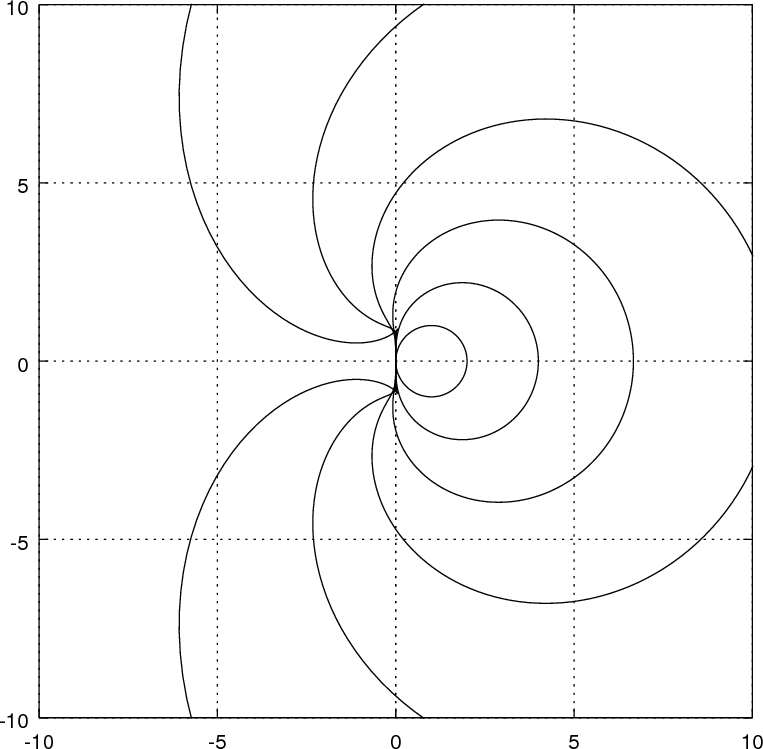
\includegraphics[width=.45\textwidth]{fig/stability-bdf.png}
  \hfill
  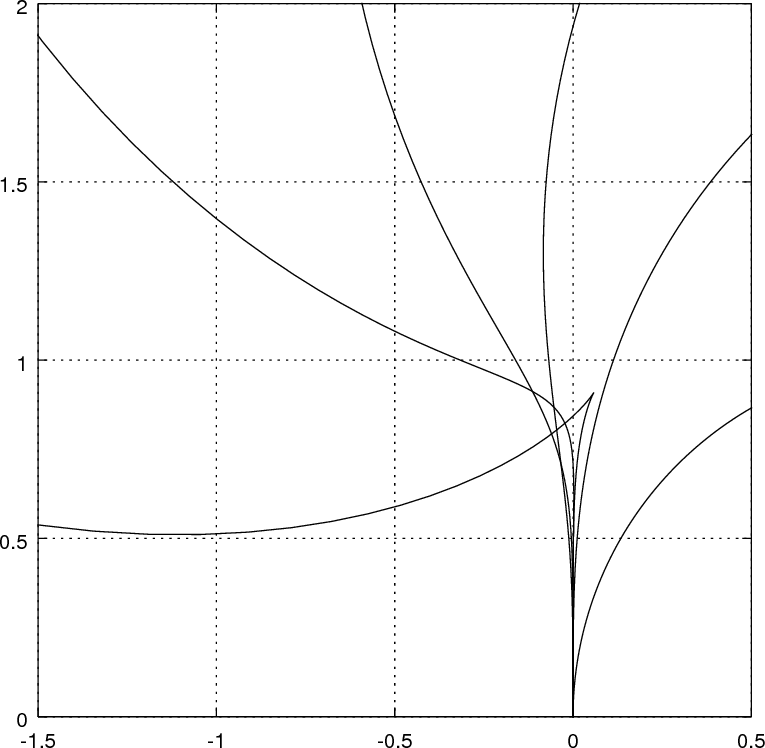
\includegraphics[width=.45\textwidth]{fig/stability-bdf-zoom.png}
  \caption{Boundaries of stability regions of BDF1 to BDF6. Unstable
    region right of the origin. Zoom on the right}
  \label{fig:bdf-stability}
\end{figure}
\begin{table}[tp]
  \centering
  \begin{tabular}{c|cccccc}
    $k$ & 1 & 2 & 3 & 4 & 5 & 6 \\\hline
    $\alpha$ & 90$^\circ$ & 90$^\circ$& 86.03$^\circ$
                    & 73.35$^\circ$& 51.84$^\circ$
                            & 17.84$^\circ$ \\
    $D$ & 0 & 0 & 0.083& 0.667& 2.327& 6.075
  \end{tabular}
  \caption{Values for A($\alpha$)- and stiff stability for BDF methods
    of order $k$.}
  \label{tab:bdf-stability}
\end{table}

%%%%%%%%%%%%%%%%%%%%%%%%%%%%%%%%%%%%%%%%%%%%%%%%%%%%%%%%%%%%%%%%%%%%%%
\section{Predictor-corrector schemes}

\begin{Definition*}{predictor-corrector}{Predictor-corrector methods}
  Assume a pair of time stepping schemes, one explicit, one implicit,
  \begin{align*}
    \hat y_{k} &= \hat \verfahren_p(y_{k-1}) \\
    y_k &= \verfahren_c(y_{k-1},y_{k}),
  \end{align*}
  we can use $\hat y_k$ as initial value for the Newton iteration for
  $y_k$. In an extreme case, we let
  \begin{gather*}
    y_k = \verfahren_c(y_{k-1},\hat y_{k}),
  \end{gather*}
  without any further iteration.
\end{Definition*}

\begin{remark}
  Predictor-corrector methods were developed strongly around
  Adams-Moulton and Adams-Bashforth methods, since the implicit ones
  have much smaller error constants. Given that these methods offer no
  considerable advantages compared to Runge-Kutta methods, but
  stability properties and implementation are weak points, We omit
  their discussion.

  A simple predictor for BDF methods can be obtained, since they are
  based on an interpolating polynomial. Thus, we simply extrapolate
  this polynomial to the next point in time.
\end{remark}

\begin{example}
  While the predictor-corrector idea sounds reasonable, we have to be
  careful with stiff problems, the original reason for using implicit
  methods. Take again our favorite IVP
  \begin{gather*}
    u' = \lambda u,
    \qquad u(0) = 1.
  \end{gather*}
  We apply the BDF(1) scheme, namely the implicit Euler method, with
  step size 1. According to its stability
  function~\eqref{eq:impl:stabil:impleuler}, we obtain
  \begin{gather*}
    y_1 = \frac1{1-\lambda}.
  \end{gather*}
  Hence, the interpolating polynomial is
  \begin{gather*}
    y(t) = (1-t) + \frac1{1-\lambda} t = 1 + \frac{\lambda}{1-\lambda}t.
  \end{gather*}
  For the mildly stiff problem $\lambda = -3$, we obtain
  \begin{gather*}
    y_1 = 0.25, \qquad y_2 = 0.0625,
    \qquad \hat y_2 = y(2) = -0.5.
  \end{gather*}
  Thus, the extrapolated value is already a much worse initial value
  for a Newton iteration than using the value from the previous time
  step.
  
  While this example was particularly chosen to exhibit such failure,
  it does show that extrapolation of stiff problems has its
  pitfalls. Here, we end up with a time step restriction which is
  comparable to the stability condition of the explicit method.
\end{example}


%%% Local Variables: 
%%% mode: latex
%%% TeX-master: "notes"
%%% End: 

\chapter{Boundary Value Problems}
\label{chapter:rwa}
\section{Introduction}
\begin{intro}
  This chapter deals with problems of a fundamentally different type
  than the problems we examined in chapter~\ref{cha:awa} and which we
  solved with previous numerical methods, namely boundary value
  problems. Here, we have prescribed values at the beginning and at
  the end of an interval of interest.

  The representation we use here is based primarily
  on~\cite{DeuflhardBornemann08} and~\cite{Rannacher12}.
\end{intro}

\begin{Definition}{bvp}
  \index{BVP|see{boundary value problem}}
  A \define{boundary value problem} (BVP) is a differential equation
  problem of the form: Find $u:[a,b]\to \R^d$, such that
  \begin{subequations}
    \label{eq:rwa:1}
    \begin{xalignat}{2}
      \label{eq:rwa:2}
      u'(t) &= f\bigl(t,u(t)\bigr)
      & t &\in (a,b) \\
      \label{eq:rwa:3}
      r\bigl(u(a), u(b)\bigr) &= 0.
    \end{xalignat}
  \end{subequations}
\end{Definition}

%%% Local Variables: 
%%% mode: latex
%%% TeX-master: "../notes"
%%% End: 

\begin{Definition}{bvp-linear}
  A BVP~\eqref{eq:rwa:1} is called linear, if the right hand side 
  $f$ as well as the boundary conditions are linear in $u$. It has the form:
  find $u:[a,b]\to \R^d$, such that
  \begin{subequations}
    \label{eq:rwa:6}
    \begin{xalignat}{2}
      \label{eq:rwa:7}
      u'(t) &= A(t)u(t) + b(t) & \forall t &\in (a,b) \\
      \label{eq:rwa:8}
      \rwaa u(a) + \rwab u(b) &= g.
    \end{xalignat}
  \end{subequations}
\end{Definition}

%%% Local Variables: 
%%% mode: latex
%%% TeX-master: "../notes"
%%% End: 


\begin{remark}
  Since boundary values are imposed at two different
  points in time, the concept of local solutions from
  definition~\ref{def:awa:local solution} is not applicable.
  Thus, tricks as going forward from interval to interval, which is
  for instance done with Euler's method in the proof of Péano's
  theorem, are here not applicable.  For this reason nothing can be
  concluded with the local properties of the right hand side $f$ at
  the points $a$ and $b$. In fact, it is just possible in a few
  special cases to conclude that a solution exists.
\end{remark}

\section{Derivatives of the solutions of IVP with respect to data}
\subsection{Derivatives with respect to the initial values}
\begin{intro}
  In order to understand BVP, we have to introduce the notion of the
  derivative of the solution to an IVP with respect to its initial
  values. We will thus denote in these cases $u=u(t;v)$, where $t$ is
  the usual ``time'' variable and $v$ the initial value, which now is
  a variable as well. Thus, $u(t;v)$ is the solution to the IVP
  \begin{gather}
    \label{eq:derivatives:1}
    \begin{split}
      u'(t;v) = \tfrac{\partial}{\partial t} u(t;v) &= f\bigl(t,u(t;v)\bigr) \\
      u(t_0;v) &= v.
    \end{split}
  \end{gather}
  The purpose of this section is the study of the derivative
  \begin{gather*}
    \tfrac{\partial}{\partial v} u(t;v),
  \end{gather*}
  which is fundamentally different from $\partial/\partial t
  u(t;v)$.
  It can be obtained by solving the variational equation of the
  original IVP, defined as follows.
\end{intro}

% \begin{remark}
%   In terms of linear \putindex{perturbation theory} this section deals
%   with the derivative of the solution $u(t)$ of the
%   IVP~\eqref{eq:awa}, but not with respect to the argument $t$, but
%   rather with respect to the initial values. That is why we will write
%   the solution $u = u(t;s)$ of the IVP
%   \begin{gather}
%     \label{eq:derivatives:1}
%     \begin{split}
%       u'(t;s) = \tfrac{\partial}{\partial t} u(t;s) &= f\bigl(t,u(t;s)\bigr) \\
%       u(t_0;s) &= s_0
%     \end{split}
%   \end{gather}
%   with two arguments, the actual time variable $t$ and the initial value $s$.
% \end{remark}

\begin{Definition}{variational-equation}
  The \define{variational equation} to the first order system of
  ODE
  \begin{gather*}
    u' = f,
  \end{gather*}
  of dimension $d$ is the linear matrix-valued system of ODE
  \begin{subequations}
  %  \label{eq:derivatives:1}
  \begin{gather}
    \label{eq:derivatives:2}
      \fundam' = \nabla_u f\bigl(t,u(t)\bigr) \fundam
  \end{gather}
  for $d\times d$ matrices $\fundam$. Here is $u$ a solution of the
  equation~\eqref{eq:awa:ode} and 
  \begin{gather*}
    \nabla_u f(t,u) =
    \begin{pmatrix}
      \tfrac{\partial f_1}{\partial u_1} & \cdots
      & \tfrac{\partial f_1}{\partial u_d} \\
      \vdots & & \vdots \\
      \tfrac{\partial f_d}{\partial u_1} & \cdots
      &  \tfrac{\partial f_d}{\partial u_d}
    \end{pmatrix}
  \end{gather*}
  is the matrix of the derivatives of $f$ with respect to the
  components of $u$. The \define{fundamental matrix}
  $\fundamental(t;t_0)$\index{Y@$\fundamental(t;t_0)$} is solution of
  the IVP to this equation with
  \begin{gather}
    \label{eq:derivatives:3}
    \fundam(t_0) = \identity.
  \end{gather}
  \end{subequations}
\end{Definition}


\begin{remark}
  The fundamental matrix $\fundam$ can also be read column
  by column.  Then each column is a vector-valued function
  $\phi^{(i)}(t)$ and solves the IVP
  \begin{gather*}
    \begin{split}
      \tfrac{d}{dt}\phi^{(i)}(t) &= \nabla_u
      f\bigl(t,u(t)\bigr)\phi^{(i)}(t),
      \\
      \phi^{(i)}(t_0) &= e_i.
    \end{split}
  \end{gather*}
\end{remark}

\begin{remark}
  The definition of the fundamental matrix here is consistent with the
  one in Definition~\ref{definition:fundamental-system} for linear
  equations. Namely, for $f(u) = Au$, we have $\nabla_u f(u) = A$.
\end{remark}

\begin{Lemma}{fundamental}
  For fundamental matrices there hold the relations
  \begin{align}
    \fundamental(t;s) &= \fundamental(s;t)^{-1}\\
    \label{eq:derivatives:4}
    \fundamental(t;r) &= \fundamental(t;s)\fundamental(s;r),
  \end{align}
  where $r,s,t$ are arbitrary real numbers, such that the solution $u$
  of the original IVP exists on the maximal interval spanned by these
  numbers.
\end{Lemma}

%%% Local Variables: 
%%% mode: latex
%%% TeX-master: "../notes"
%%% End: 


\begin{proof}
  In order to prove the first equation, denote by $V(\tau;s)$ the
  solution to the IVP
  \begin{gather*}
    V'(\tau;s) = \nabla_u f(\tau,u(\tau)) V(\tau;s),
    \qquad V(s;s) = \fundamental(s;t).
  \end{gather*}
  Because of uniqueness, we must have
  $V(\tau;s) = \fundamental(\tau;t)$ for any $\tau$ between $s$ and
  $t$, in particular for $r=t$, such that $V(t;s) = \identity$. On the
  other hand, by linearity, we have
  $V(\tau;s) = \fundamental(\tau;s)\fundamental(s;t)$, and thus the
  equation is proven by
  \begin{gather*}
    \identity = V(t;s) = \fundamental(t;s)\fundamental(s;t).
  \end{gather*}

  Now, assume without loss of generality that $s$ is between $r$ and
  $t$. Indeed, if for instance $t$ is between $r$ and $s$, multiply
  equation~\eqref{eq:derivatives:4} from the left by $U(s;t)$ and
  prove the equation for
  \begin{gather*}
    U(s;t)U(t;r) = U(s;t)U(t;s)U(s;r) = U(s;r).
  \end{gather*}
  Take the auxiliary function $V(\tau;s)$ as defined above. By
  uniqueness, it is equal to $U(\tau;t)$ for all $\tau$. But, on the
  other hand, we have by linearity $V(\tau;s) = U(\tau;s)U(s;r)$, in
  particular for $\tau=t$.

  The statement follows from the definition as a solution of an IVP
  and the fact that solutions of linear IVP are linear combinable.
\end{proof}

\begin{Theorem}{derivative}
  \index{conditioning!AWA} Let be $f(t,u)$ continuous in $t$ and
  continuously differentiable in $u$.  Then, the solution $u(t;v)$ of
  the IVP~\eqref{eq:derivatives:1} depends differentiably on the
  initial value $v$ and the derivative is given by
  \begin{gather}
    \label{eq:derivatives:5}
    \tfrac{\partial}{\partial v} u(t;v) = \fundamental(t;t_0),
  \end{gather}
  where $\fundamental(t;t_0)$ is the fundamental matrix with respect
  to the initial time $t_0$.
\end{Theorem}



\begin{proof}
  We write the IVP in its full dependence on $v$ as
  \begin{align*}
    \frac{\partial u(t;v)}{\partial t} &= f\bigl(t,u(t;v)\bigr) \\
    u(t_0;v) &= v.
  \end{align*}
  From the second equation, we immediately obtain
  \begin{gather*}
    \frac{\partial u(t_0;v)}{\partial v} = \identity.
  \end{gather*}
Assuming differentiability of $f$ with respect to $u$, the first
equation yields
\begin{gather*}
  \frac{\partial}{\partial v}\frac{\partial u(t;v)}{\partial t}
  = \frac{\partial f\bigl(t,u(t;v)\bigr)}{\partial v}
  = \nabla_u f(t,u(t;v)) \frac{\partial u(t;v)}{\partial v}.
\end{gather*}
Thus, $\nicefrac{\partial}{\partial v} u$ solves the
IVP~\eqref{eq:derivatives:1}. Since the solution exists and is unique,
this derivative is well defined and thus, the function is differentiable.
\end{proof}

\subsection{Derivatives with respect to the right hand side function}
\begin{intro}
  We close this section by studying the differential dependence of the
  solution $u(t)$ of an ODE at time $t$ on the function $f(t,u)$, that
  is, the derivative of a value with respect to a function. In order
  to keep things simple, we reduce this question to a regular
  derivative of a function with respect to a real variable by using
  the Gâteaux derivative. To this end, let $F(v)$ be a functional on
  some function space, that is, a real valued function on this
  space. Then, the Gâteaux derivative of $F$ at a point $v$ in
  direction $w$ with $v$ and $w$ in this function space is defined as
  \begin{gather}
    \label{eq:derivatives:6}
    \frac{\partial}{\partial w} F(v)
    = \lim_{\epsilon\to 0} \frac{F(v+\epsilon w) - F(v)}{\epsilon}.
  \end{gather}
  Here, we have used the notation for directional derivatives in
  $\R^n$, since this is indeed the character of the Gâteaux
  derivative.

  Back to differential equations, our task is now to compute the
  derivative of $u(t)$ with respect to changes in $f$, denoted as
  \begin{gather}
    \label{eq:derivatives:7}
    \frac{\partial}{\partial g} u(t)
    = \lim_{\epsilon\to 0} \frac{u_\epsilon-u}{\epsilon}
    = \left.\frac{d}{d\epsilon} u_\epsilon(t)\right|_{\epsilon=0},
  \end{gather}
  where $u$ and $u_\epsilon$ respectively solve the IVPs
  \begin{xalignat*}{2}
    u'&=f(t,u) & u(t_0)& = u_0 \\
    u_\epsilon'&=f(t,u_\epsilon)+\epsilon g(t,u_\epsilon)
    & u_\epsilon(t_0)& = u_0.
  \end{xalignat*}
  For this derivative, we have the following theorem.
\end{intro}

\begin{Theorem}{derivative-f}
  Let $f(t,u)$ and $g(t,u)$ be continuous in their first and
  continuously differentiable in their second argument. Let $u$ be the
  solution of the IVP $u'=f(u)$ with $u(t_0) = u_0$. Then, the Gâteaux
  derivative of $u$ in $f$ with respect to a perturbation $g$ exists
  and there holds
  \begin{gather}
    \label{eq:derivative-f:1}
    \frac{\partial}{\partial g} u(t)
    = \int_{t_0}^t \fundamental(t;s) g\bigl(s,u(s)\bigr)\, \ds.
  \end{gather}
\end{Theorem}
%%% Local Variables:
%%% mode: latex
%%% TeX-master: "../notes"
%%% End:


\begin{proof}
  We set out by devising a differential equation for the Gâteaux
  derivative $\mathcal U(t)$. The differential equation for $u$ yields
  \begin{multline*}
    \mathcal U(t) := \left.\frac{d}{d\epsilon} u_\epsilon(t)\right|_{\epsilon=0}
    = \left.\frac{d}{d\epsilon}
    \Bigl(f\bigl(t,u_\epsilon(t)\bigr)
    + \epsilon g\bigl(t,u_\epsilon(t)\bigr)\Bigr) \right|_{\epsilon=0}
  \\
    = \left.\nabla_u f(t,u_\epsilon) \mathcal U(t)
    + g\bigl(t,u_\epsilon(t)\bigr) \right|_{\epsilon=0}
  \end{multline*}
  Furthermore, we have
  \begin{gather*}
     \mathcal U(t_0) = \frac{d}{d\epsilon} u_\epsilon(t_0) = 0.
  \end{gather*}

  According to Lemma~\ref{lemma:linear-representation}, the solution
  of this initial value problem can be represented with the
  integrating factor $M(t)$ as
  \begin{gather*}
    \mathcal U(t) = M^{-1}(t) \int_{t_0}^t M(s) g\bigl(s,u(s)\bigr)
    \,d s.
  \end{gather*}
  Noticing that $M(\tau)^{-1} = U(\tau;t_0)$, we obtain
  \begin{gather*}
    u(t) = \int_{t_0}^t \fundamental(t;s) g\bigl(s,u(s)\bigr) \,d s
  \end{gather*}
\end{proof}


%%% Local Variables: 
%%% mode: latex
%%% TeX-master: "notes"
%%% End: 

%%%%%%%%%%%%%%%%%%%%%%%%%%%%%%%%%%%%%%%%%%%%%%%%%%%%%%%%%%%%%%%%%%%%%%
%%%%%%%%%%%%%%%%%%%%%%%%%%%%%%%%%%%%%%%%%%%%%%%%%%%%%%%%%%%%%%%%%%%%%%
\section{Theory of boundary value problems}
%%%%%%%%%%%%%%%%%%%%%%%%%%%%%%%%%%%%%%%%%%%%%%%%%%%%%%%%%%%%%%%%%%%%%%
%%%%%%%%%%%%%%%%%%%%%%%%%%%%%%%%%%%%%%%%%%%%%%%%%%%%%%%%%%%%%%%%%%%%%%

\begin{remark}
  The very general boundary condition (BC) \index{Boundary
    condition}~\eqref{eq:rwa:3} usually has more simple forms. Often
  it is a \textbf{linear} \putindex{linear boundary condition}
   which we can note in the following form
  \begin{gather}
    \label{eq:rwa:4}
    \rwaa u(a) + \rwab u(b) = g
  \end{gather}
  with $d\times d$ matrices $\rwaa$ and $\rwab$ as well as a vector $g\in
  \R^d$. Another very common case is the one of 
  \textbf{separated}
  \index{boundary condition!separated}
  \index{separated boundary condition}
  boundary conditions, which has the form
  \begin{xalignat}{2}
    \label{eq:rwa:5}
    r_a\bigl(u(a)\bigr) &= 0,
    &
    r_b\bigl(u(b)\bigr) &= 0,
    \\\intertext{or}
    \rwaa u(a) &= g_a,
    &
    \rwab u(b) &= g_b.
  \end{xalignat}
\end{remark}

\begin{example}
  Take the second order differential equation
  \begin{gather*}
    u''(t) = -2, \quad \forall t\in (0,1),
  \end{gather*}
  with boundary conditions
  \begin{gather*}
    u(0) = u(1) = 0.
  \end{gather*}
  We can deduce from the differential equation that the solution is a
  parabola open to the bottom, and we verify easily that
  \begin{gather*}
    u(t) = t(1-t)
  \end{gather*}
  is a solution.
\end{example}

\begin{example}
  Take the first order differential equation
  \begin{gather*}
    u'(t) = u(t), \quad \forall t\in (0,1),
  \end{gather*}
  with boundary values
  \begin{gather*}
    u(0) = u(1) = 1.
  \end{gather*}
  From the theory of the first chapter, we know that the initial value
  problem with only the initial value at zero has the unique solution
  $u(t) = e^t$. Thus, this BVP does not have a solution.

  If we changed the condition at the right end of the interval to
  $u(1) = e$, the problem is solvable, albeit we have to admit that
  this solution seems somewhat accidental.
\end{example}

%%%%%%%%%%%%%%%%%%%%%%%%%%%%%%%%%%%%%%%%%%%%%%%%%%%%%%%%%%%%%%%%%%%%%%
\begin{remark}
  As the examples show, a satisfying theory for the existence of
  solutions will be difficult to obtain for any boundary values. For
  instance, in the linear case it is obvious that neither $\rwaa$, nor
  $\rwab$ may have full rank, because that would imply the unique
  existence either of the IVP with $\rwaa u(a) = g_a$ or
  $\rwab u(b) = g_b$, and thus no freedom to match the condition at
  the other end.

  As a consequence we now turn our attention to a ``restricted''
  solution theory and wonder: assume a solution of the problem
  exists. Which further conditions are necessary to obtain
  well-posedness of the problem in terms of Hadamard
  (definition~\vref{Definition:hadamard}).

  The key is the following definition which grants us the possibility
  of the approximation of a solution, at least after a quantification
  of the neighborhood.
\end{remark}

%%%%%%%%%%%%%%%%%%%%%%%%%%%%%%%%%%%%%%%%%%%%%%%%%%%%%%%%%%%%%%%%%%%%%% 
\begin{Definition}{local-uniqueness}
  \defindex{solution!locally unique (BVP)} A solution $u(t)$ of the
  BVP~\eqref{eq:rwa:1} is called \textbf{locally unique}
  \defindex{locally unique solution (BVP)} or
  \textbf{isolated}\defindex{isolated solution}, if there is no second
  solution $v(t)$ of the BVP, which is arbitrary close to $u(t)$. In
  mathematical language: there exists an $\epsilon>0$, such that for
  any two solutions of the BVP there holds
  \begin{gather*}
    \max_{t\in [a,b]}|u(t)-v(t)| < \epsilon
    \qquad\Rightarrow\qquad
    u(t) = v(t) \quad \forall t\in [a,b].
  \end{gather*}
\end{Definition}

%%%%%%%%%%%%%%%%%%%%%%%%%%%%%%%%%%%%%%%%%%%%%%%%%%%%%%%%%%%%%%%%%%%%%%
\begin{Lemma}{bvp-derivative}
  Let be $f(t,u)$ continuous in $t$ and continuously differentiable in
  $u$.  Let additionally $r(x,y)$ be continuously differentiable and
  set
  \begin{gather}
    \label{eq:rwa:9}
    \rwaa = \left.\frac{\partial r(x,y)}{\partial
        x}\right|_{x=u(a),y=u(b)},
    \qquad
    \rwab = \left.\frac{\partial r(x,y)}{\partial
        y}\right|_{x=u(a),y=u(b)}.
  \end{gather}
  Let $u(t)$ be a continuously differentiable solution of the
  BVP~\eqref{eq:rwa:1}.  Then the derivative of the boundary condition
  $r(u(a),u(b))$ with respect to the function value $u(t)$ inside the
  interval $[a,b]$ is
  \begin{gather}
    \label{eq:rwa:12}
    E(t)
    := \frac{\partial r\bigl(u(a),u(b)\bigr)}{\partial u(t)}
    = \rwaa \fundamental(a;t) + \rwab \fundamental(b;t),
  \end{gather}
  where $\fundamental(t;t_0)$ is the fundamental matrix.
\end{Lemma}


\begin{remark}
  The definition of the matrices $\rwaa$ and $\rwab$ above is
  consistent with the usage of the matrix $\rwaa$ and $\rwab$ in
  equation~\eqref{eq:rwa:4}.
\end{remark}

\begin{proof}
  We consider the auxiliary function $w_t(\tau;v)$ as solution of the
  IVP with initial value $v$ in $t$:
  \begin{gather*}
    \frac{\partial}{\partial \tau} w_t(\tau;v)
    = f\bigl(\tau,w_t(\tau;v)\bigr), \qquad w_t(t;v) = v.
  \end{gather*}
  Choosing $v=u(t)$, we have by uniqueness $w_t(a;v) = u(a)$ and
  $u(b) = w_t(b;v)$. Our task of computing the derivative with respect
  to $u(t)$ has thus become computing the derivative with respect to
  $v$. The derivative of the boundary condition can therefore be
  written as
  \begin{align*}
    \frac{\partial r\bigl(u(a),u(b)\bigr)}{\partial u(t)}
    &=
    \frac{\partial r\bigl(w_t(a;v),w_t(b;v)\bigr)}{\partial v}
    \\
    &= \rwaa \frac{\partial w_t(a;v)}{\partial v}
    + \rwab \frac{\partial w_t(b;v)}{\partial v}
    \\
    &= \rwaa \fundamental(a;t) + \rwab \fundamental(b;t),
  \end{align*}
  where the last equality is due to Theorem~\ref{Theorem:derivative}.
\end{proof}

\begin{remark}
  In order to study local uniqueness of solutions and well-posedness
  of BVP, we have to change our view on boundary conditions and
  consider them as functions of solutions to the differential
  equation. Thus, we will consider the function
  \begin{gather*}
    \rho(v) := r\bigl(v(a),v(b)\bigr),
  \end{gather*}
  mapping solutions of the differential equation to their boundary
  values. $\rho$ is a continuous function, and, as the following
  theorem shows, even differentiable.
\end{remark}

\begin{Definition}{local-uniqueness}
  \defindex{solution!locally unique (BVP)} A solution $u(t)$ of the
  BVP~\eqref{eq:rwa:1} is called \textbf{locally unique}
  \defindex{locally unique solution (BVP)} or
  \textbf{isolated}\defindex{isolated solution}, if there is no second
  solution $v(t)$ of the BVP, which is arbitrary close to $u(t)$. In
  mathematical language: there exists an $\epsilon>0$, such that for
  any two solutions of the BVP there holds
  \begin{gather*}
    \max_{t\in [a,b]}|u(t)-v(t)| < \epsilon
    \qquad\Rightarrow\qquad
    u(t) = v(t) \quad \forall t\in [a,b].
  \end{gather*}
\end{Definition}


\begin{proof}
  First assume that $E(t)$ is regular for some $t$. Then we have for
  $\tau \neq t$:
  \begin{align*}
    E(\tau) &= \rwaa \fundamental(a;\tau) + \rwab \fundamental(b;\tau)
    \\
    &= \rwaa \fundamental(a;t)\fundamental(t;\tau) + \rwab
    \fundamental(b;t)\fundamental(t;\tau)
    = E(t) \fundamental(t;\tau),
  \end{align*}
  where the first factor is regular by assumption, the second one as the
  fundamental matrix of a linear ODE.

  Now, we consider the matrix $E(t)=E_u(t)$ as a function of $u(t)$, which is
  continuous by assumption. Therefore, if it is regular in $u(t)$, it
  is regular in a neighborhood of $u(t)$ of some positive diameter
  $\epsilon$. Let now $v$ be a second solution of the differential
  equation with $\abs{u(t)-v(t)}<\epsilon$. Then,
  \begin{gather*}
    \rho(u)-\rho(v) = E_\phi(t) \bigl(u(t)-v(t)\bigr),
  \end{gather*}
  where $\phi(t)$ is between $u(t)$ and $v(t)$ and thus $E_\phi(t)$ is
  regular. If both functions solve the BVP, then the left hand side is
  zero, and thus $v(t)=u(t)$.
\end{proof}

Now that we established the local uniqueness of the solution,
it yet remains to show the continuous dependency of data (stability).  
Here we are in particular interested, in analogy to the 
stability theorem, in the derivative
of the solution at time $t$ after perturbations of values on the boundary. 
For this purpose we have:

\begin{Theorem}{bvp-stability-1}
  \index{conditioning!BVP}
  Let the assumptions of Lemma~\ref{Lemma:bvp-derivative} hold and let
  $u(t)$ be the solution of the BVP~\eqref{eq:rwa:1} with
  \begin{gather*}
    u(a) = g_a\quad \text{and} \quad u(b) = g_b.
  \end{gather*}
  Then, there holds
  \begin{gather}
    \label{eq:rwa:20}
    \frac{\partial u(t)}{\partial g_a} = E^{-1}(t) \rwaa,
    \qquad
    \frac{\partial u(t)}{\partial g_b} = E^{-1}(t) \rwab.
  \end{gather}
  In particular, the conditioning with respect to changes of size
  $\epsilon$ in the boundary conditions $g_a$ and $g_b$ is
  \begin{gather}
    \delta u(t) \le \epsilon
    \max\bigl\{\norm{E^{-1}(t) \rwaa}, \norm{E^{-1}(t)\rwab}\bigr\}.
  \end{gather}
\end{Theorem}


\begin{proof}
  We demonstrate the proof for the derivative with respect to the left
  boundary value. The second equation can be proven the same way.
  With the chain rule we obtain
  \begin{gather*}
    \frac{\partial u(t)}{\partial g_a}
    = \frac{\partial u(t)}{\partial r(g_a,g_b)}
    \frac{\partial r(g_a,g_b)}{\partial g_a}
  \end{gather*}
  The second derivative is~\eqref{eq:rwa:9} $\rwaa$. For the first one
  we notice that $E(t)$ is the derivative of the inverse mapping of
  $\rho(u)$. By application of the implicit function theorem, we
  obtain the result.
\end{proof}

% \begin{example}
%   Consider the second order boundary value problem
%   \begin{gather*}
%     u'' = k^2 u,
%     \qquad u(a) = g_a, \quad u(b) = g_b.
%   \end{gather*}
%   We convert this into the system
%   \begin{gather*}
%     \frac{d}{dt}
%     \begin{pmatrix}
%       u_1 \\ u_2
%     \end{pmatrix}
%     =
%     \begin{pmatrix}
%       & k \\ k
%     \end{pmatrix}
%     \begin{pmatrix}
%       u_1 \\ u_2
%     \end{pmatrix}.
%   \end{gather*}
%   The fundamental matrix is
%   \begin{gather}
%     \label{eq:rwa:10}
%     \fundamental(\tau;t) =
%     \begin{pmatrix}
%       e^{k(\tau-t)} & e^{k(t-\tau)} \\
%       ke^{k(\tau-t)} & - ke^{k(t-\tau)}
%     \end{pmatrix}.
%   \end{gather}
% \end{example}

\begin{Theorem}{bvp-stability-2}
  Let $f(t,u)$ and $g(t,u)$ be continuous in $t$ and continuously
  differentiable in $u$. Then, the variation of the value $u(t)$ of
  the solution $u$ of the boundary value problem
  \begin{gather*}
    u'=f(t,u),\qquad r\bigl(u(a), u(b)\bigr)=0,
  \end{gather*}
  with respect to perturbations $f+g$ is
  \begin{gather}
    \label{eq:bvp-stability-2:1}
    \frac{\partial}{\partial g} u(t)
    = \int_{a}^b G(t,s) g\bigl(s,u(s)\bigr)\,d s,
  \end{gather}
  where
  \begin{gather}
    \label{eq:bvp-stability-2:2}
    G(t,s) =
    \begin{cases}
      -E(t)^{-1} \rwaa \fundamental(a;s) & a \le s \le t \\
      \phantom{-}E(t)^{-1} \rwab \fundamental(b;s) & t < s \le b
    \end{cases}.
  \end{gather}
\end{Theorem}

%%% Local Variables:
%%% mode: latex
%%% TeX-master: "../notes"
%%% End:


\begin{proof}
  We begin by estimating the influence of perturbations of the right
  hand side on the boundary values. Using the corresponding
  Theorem~\ref{Theorem:derivative-f} for IVP, where we swap the
  meaning of $t$ and the interval boundaries, we obtain
  \begin{align*}
    \frac{\partial u(a)}{\partial g}
    &= \int_t^a \fundamental(a;s) g\bigl(s,u(s)\bigr) \ds,
    \\
    \frac{\partial u(b)}{\partial g}
    &= \int_t^b \fundamental(b;s) g\bigl(s,u(s)\bigr) \ds,
  \end{align*}
  By the chain rule and Lemma~\ref{Lemma:bvp-derivative}
  and Theorem~\ref{Theorem:bvp-stability-1}, we get
  \begin{gather*}
    \frac{\partial r\bigl(u(a), u(b)\bigr)}{\partial g}
    = \frac{\partial r\bigl(u(a), u(b)\bigr)}{\partial u(t)}
    \frac{\partial u(t)}{\partial g}
    = E(t)\frac{\partial u(t)}{\partial g}.
  \end{gather*}
Assembling everything, we obtain
\begin{multline*}
  \frac{\partial u(t)}{\partial g}
  = E(t)^{-1} \frac{\partial r\bigl(u(a), u(b)\bigr)}{\partial g}
  = E(t)^{-1} \left(
    \rwaa \frac{\partial u(a)}{\partial g}
    + \rwab \frac{\partial u(b)}{\partial g}\right)
  \\
  = E(t)^{-1} \left(
    \rwaa \int_t^a \fundamental(a;s) g\bigl(s,u(s)\bigr) \ds
    + \rwab \int_t^b \fundamental(b;s) g\bigl(s,u(s)\bigr) \ds
    \right).
  \end{multline*}
\end{proof}

\begin{remark}
  Theorems~\ref{Theorem:local-uniqueness}, \ref{Theorem:bvp-stability-1}
  and~\ref{Theorem:bvp-stability-2} represent the verification of the
  second and third Hadamard conditions\index{Hadamard conditions}.
  Thus, even if the existence of a solution for the BVP is not always
  guaranteed, solutions can be approximated under certain conditions.
  
  The case for linear boundary value problems is much simpler and we
  have an existence an uniqueness result.
\end{remark}

\begin{Definition}{bvp-linear}
  A BVP~\eqref{eq:rwa:1} is called linear, if the right hand side 
  $f$ as well as the boundary conditions are linear in $u$. It has the form:
  find $u:[a,b]\to \R^d$, such that
  \begin{subequations}
    \label{eq:rwa:6}
    \begin{xalignat}{2}
      \label{eq:rwa:7}
      u'(t) &= A(t)u(t) + b(t) & \forall t &\in (a,b) \\
      \label{eq:rwa:8}
      \rwaa u(a) + \rwab u(b) &= g.
    \end{xalignat}
  \end{subequations}
\end{Definition}

%%% Local Variables: 
%%% mode: latex
%%% TeX-master: "../notes"
%%% End: 


\begin{proof}
  By Theorem~\ref{Lemma:bvp-derivative} and linearity of the BVP,
  we deduce that the mapping $\rho$ from $u(t)$ to the boundary
  condition is affine and can be written in the form
  \begin{gather*}
    r\bigl(u(a),u(b)\bigr) = E(t) u(t) + b(t),
  \end{gather*}
  where $b(t)$ is some vector in $\R^d$ or $\C^d$ independent of
  $u$. Since everything in this equation exept $u(t)$ is given, the
  unique solvability is equivalent to the invertibility of $E(t)$,
  which by Theorem~\ref{Theorem:local-uniqueness} is equivalent to
  regularity of $E(a)$ .
\end{proof}


%%%%%%%%%%%%%%%%%%%%%%%%%%%%%%%%%%%%%%%%%%%%%%%%%%%%%%%%%%%%%%%%%%%%%%
%%%%%%%%%%%%%%%%%%%%%%%%%%%%%%%%%%%%%%%%%%%%%%%%%%%%%%%%%%%%%%%%%%%%%%
\section{Shooting methods}
\subsection{Single shooting method}
%%%%%%%%%%%%%%%%%%%%%%%%%%%%%%%%%%%%%%%%%%%%%%%%%%%%%%%%%%%%%%%%%%%%%%
%%%%%%%%%%%%%%%%%%%%%%%%%%%%%%%%%%%%%%%%%%%%%%%%%%%%%%%%%%%%%%%%%%%%%%

\begin{example}
  We illustrate the shooting method on a simple, scalar example
  \begin{gather*}
    u'' = -g, \quad u(0) = 0, \quad u(1) = 0.
  \end{gather*}
	What we can solve is the IVP
  \begin{gather*}
    u'' = -g, \quad u(0) = 0, \quad u'(0) = s.
  \end{gather*}
	The latter has a unique solution u(t;s) for each initial value
  $s$. Now it is our task to find a value $s^*$, such that
  $u(1;s^*) = 0$. With other words, we search for a root of the function
  \begin{gather*}  
    F(s) = u(1;s).
  \end{gather*}
  This can be done with an arbitrary, convergent iteration method.
  For an example with the Bisection method.  Of course the Newton
  method would be a better choice but for that we need to calculate
  the derivatives of $F$.  This can be achieved with
  theorem~\ref{Theorem:derivative} by calculating the
  fundamental matrix $\fundam$.
\end{example}

\begin{Algorithm}{single-shooting}
  The single shooting method with standard \putindex{Newton method}
  consists of the following steps:
  \begin{enumerate}
  \item Start with an initial guess $v^{(0)}\in \R^d$.
  \item For $v^{(n)}$ given, solve the IVP and the associated variation equation
    \begin{xalignat*}{2}
      \tfrac\partial{\partial t}u^{(n)}(t) &=
      f\bigl(t,u^{(n)}(t)\bigr)
      & u^{(n)}(a) &= v^{(n)},\\
      \tfrac\partial{\partial t}\fundam^{(n)}(t;a)
      &= \nabla_uf\bigl(t,u^{(n)}(t)\bigr)\fundam^{(n)}(t;a)
      &\fundam^{(n)}(a;a) &= \identity.
    \end{xalignat*}
  \item Set
    \begin{gather}
      \label{eq:rwa:14}
      v^{(n+1)} = v^{(n)}
      - \bigl(\rwaa + \rwab \fundam^{(n)}(b;a)\bigr)^{-1}
      r\bigl(v^{(n)},u^{(n)}(b)\bigr)
    \end{gather}
  \item Stop the iteration if the value
    $r\bigl(s,u(t;u_0^{(n+1)})\bigr)$ is sufficiently small,\\
    otherwise repeat from 2.
  \end{enumerate}
\end{Algorithm}

%%% Local Variables:
%%% mode: latex
%%% TeX-master: "../notes"
%%% End:


\begin{remark}
  The task of the shooting method is solved normally with the help of
  Newton's method, which searches for a root (with respect to $v$) of
  the function
  \begin{gather}
    \label{eq:rwa:11}
    F(v) = r\bigl(v, u(b;v)\bigr)
  \end{gather}
	For Newton's method we require the partial derivatives
  \begin{gather*}
    \frac\partial{\partial v^{(i)}} F(v) =
    \partial_1 r\bigr(v,u(b;v)\bigr)
    + \partial_2r\bigr(v,u(b;v)\bigr) \frac\partial{\partial v^{(i)}} u(b;v),
  \end{gather*}
  % For linear and separate boundary conditions this leads to a significantly 	
  %       more readable form: 
  % \begin{gather*}
  %   \frac\partial{\partial u_0^{(i)}} F(s) = \rwaa s + \rwab
  %   \frac\partial{\partial u_0^{(i)}} u(b;u_0)
  % \end{gather*}
  which involves the \putindex{fundamental matrix} $\fundamental(b;a)$
  of derivatives of the solution at point $b$ with respect to the
  initial values (see Lemma~\ref{Lemma:bvp-derivative}).
\end{remark}

\begin{Algorithm}{single-shooting}
  The single shooting method with standard \putindex{Newton method}
  consists of the following steps:
  \begin{enumerate}
  \item Start with an initial guess $v^{(0)}\in \R^d$.
  \item For $v^{(n)}$ given, solve the IVP and the associated variation equation
    \begin{xalignat*}{2}
      \tfrac\partial{\partial t}u^{(n)}(t) &=
      f\bigl(t,u^{(n)}(t)\bigr)
      & u^{(n)}(a) &= v^{(n)},\\
      \tfrac\partial{\partial t}\fundam^{(n)}(t;a)
      &= \nabla_uf\bigl(t,u^{(n)}(t)\bigr)\fundam^{(n)}(t;a)
      &\fundam^{(n)}(a;a) &= \identity.
    \end{xalignat*}
  \item Set
    \begin{gather}
      \label{eq:rwa:14}
      v^{(n+1)} = v^{(n)}
      - \bigl(\rwaa + \rwab \fundam^{(n)}(b;a)\bigr)^{-1}
      r\bigl(v^{(n)},u^{(n)}(b)\bigr)
    \end{gather}
  \item Stop the iteration if the value
    $r\bigl(s,u(t;u_0^{(n+1)})\bigr)$ is sufficiently small,\\
    otherwise repeat from 2.
  \end{enumerate}
\end{Algorithm}

%%% Local Variables:
%%% mode: latex
%%% TeX-master: "../notes"
%%% End:


% \begin{corollary}
%   For linear a BVP~\eqref{eq:rwa:6} the initial value $v$, such that
%   $u(t;v)$ solves the BVP, is the solution of the linear system of
%   equations
%   \begin{gather}
%     \label{eq:rwa:13}
%     \bigl(\rwaa + \rwab\fundamental(b;a)\bigr) v = g - \rwab u(b;0).
%   \end{gather}
% \end{corollary}

% \begin{proof}
% 	For linear equations we know that the Newton's method converges in one step,
% 	for arbitrary initial values.
% 	We can use this to execute the upper algorithm with initial value
% 	 $u_0^{(0)} = 0$.
% 	Under application of $r(u(a),u(b)) = B_a u(a) + B_b u(b) -
%   g$ we obtain the upper formula by inserting in~\eqref{eq:rwa:14}.
% \end{proof}

\begin{remark}
  The IVP in this algorithm usually cannot be solved
  analytically. Thus, we have to use what we learned in the previous
  chapters to choose a time stepping scheme.

  Newton's method is known to converge locally, not
  globally. Therefore, a good initial value is needed for this
  algorithm to converge. This is the more true, since the solution of
  the IVP may grow much faster and may be less stable than that of the
  BVP (see homework), and is only approximated. There are two ways out
  of this problem: first, a Newton method should never be implemented
  without any globalization strategy, which modifies the update to
  increase the domain of convergence. The second part of the solution
  consists in choosing a method which is more robust than single
  shooting in the next section.
\end{remark}

\begin{remark}
  Step 2 of the single shooting algorithm requires solving the
  \putindex{variational equation} of our original ODE. If $f$
  describes a complex nonlinear process, the computation and
  implementation of its derivative may be a daunting and error prone
  task. This can be avoided by three different algorithmical
  tools. For each of them, we describe the main advantages and
  disadvantages:
  \begin{description}
  \item[Automatic differentiation] Software like for instance
    the module Sacado of the Trilinos package, has the standard rules
    of differentiation (Leibniz, quotient, chain rules, derivatives of
    polynomials and standard functions) built in. By implementing
    $f(u)$ in a conforming way, the software can automatically
    generate the code for its derivatives. Clearly, the advantage is
    that there is no approximation involved in those derivatives and
    thus equation and variational equation are always consistent. On
    the other hand, derivatives, which are not simplified
    analytically, can become fairly complex. Here, we rely on a good
    implementation of the automatic differentiation as well as on the
    optimizing capabilities of the compiler.
  \item[Internal numerical differentiation] While using a time
    stepping scheme for solving the IVP, for example a one-step
    method, in each time step, we compute
      \begin{gather*}
        y^k = \Phi(y^{k-1})
      \end{gather*}
      as well as approximations
      \begin{gather*}
        \frac{\partial}{\partial y_i} y^k
        \approx \frac{\Phi(y^{k-1}+\epsilon e_i) - \Phi(y^{k-1})}{\epsilon}
      \end{gather*}
with the same integration method $\Phi$ and the same step sizes $h_k$.       This approximation can also be replaced by more accurate
      differentiation formulas. Such an implementation requires $d$
      additional evaluations of $\Phi$ to compute the full gradient,
      which is feasible only for moderately sized $d$. Furthermore,
      the choice of $\epsilon$ is tricky, since the approximation is
      inaccurate for large values and unstable for small.
      Implementations of time stepping schemes which compute both $y$
      and its derivatives are available in the optimization community
      as well among reseach groups implementing filtering techniques
      in stochastic methods.
      
    \item[External numerical diferentiation] Here we forget about the
      variational equation altogether and approximate by difference
      quotients the derivative of $u(b)$ with respect to changes in
      the initial value directly:
      \begin{gather*}
        \frac{\partial}{\partial v_i} u(b)
        \approx \frac{u(b;v+\epsilon e_i) - u(b;v)}{\epsilon}.
      \end{gather*}
In practice, $u(b;v+\epsilon e_i)$ and $u(b;v)$ are computed numerically by any integration method and in general using different step sizes.       The robust choice of $\epsilon$ is more critical here and the
      search for a general algorithm to address this issue has
      failed. Therefore, this method is only used rarely nowadays
      (judgement from~\cite{DeuflhardBornemann08}).
  \end{description}

  A final remark on computing the Jacobian and its inverse: if an
  iterative method is used to solve the linear system in each Newton
  step, the complete matrix is not needed, but only the matrix applied
  to a direction vector. This is something that can be used to
  accelerate all methods described above by avoiding the computation
  of unneeded values.
\end{remark}

%%%%%%%%%%%%%%%%%%%%%%%%%%%%%%%%%%%%%%%%%%%%%%%%%%%%%%%%%%%%%%%%%%%%%%
%%%%%%%%%%%%%%%%%%%%%%%%%%%%%%%%%%%%%%%%%%%%%%%%%%%%%%%%%%%%%%%%%%%%%%
\subsection{Multiple shooting method}
\index{shooting method!multiple}

\begin{example}
 Take on the interval $[0,2]$ the (admittedly somewhat artificial) boundary value problem
 \begin{gather*}
   u' = u^2,\qquad u(2) = 1,
 \end{gather*}
 which has the bounded solution
 \begin{gather*}
   u(t) = \frac1{3-t}.
 \end{gather*}
 We might be tempted to start our shooting method with $v=1$ after
 realizing that $v=0$ leads nowhere. But then, we get
 \begin{gather*}
   u^{(0)}(t) = \frac1{1-t},
 \end{gather*}
 which only exists on the interval $[0,1)$. Clearly, the single
 shooting method is not suited to solve this otherwise harmless BVP.

 This observation leads to the idea of applying the shooting method on
 smaller subintervals and gluing those together.
\end{example}

\begin{Definition}{multiple-shooting}
  Choose a partitioning of the interval $[a,b]$ such that
  \begin{gather*}
    a=t_0<t_1<t_2<\dots<t_m=b.
  \end{gather*}
  On each subinterval $I_k = [t_{k-1}, t_k]$, $k=1,\ldots,m$ define
  the IVP
  \begin{gather*}
    u_k' = f(t, u_k), \qquad u_k\bigl(t_{k-1}\bigr) = v_k,
  \end{gather*}
  The \define{multiple shooting method} consists of finding vectors
  $v_1,\dots, v_m$, such that
  \begin{xalignat*}{2}
    v_{k+1}&= u_{k}\bigl(t_{k}\bigr)& k&=1,\dots,m-1,\\
    r(v_1, u_m(b)) &= 0.
  \end{xalignat*}
  The function
  \begin{gather*}
    u(t) = u_k(t) \qquad\text{for } t\in I_k
  \end{gather*}
  is continuous, solves the ODE, and obeys the boundary conditions.
\end{Definition}

%%% Local Variables:
%%% mode: latex
%%% TeX-master: "../notes"
%%% End:


\begin{remark}
  The numbering of intervals, vectors, and time partitioning has been
  chosen to be consistent with the previous definitions in this
  class. The governing entity is the subinterval $I_k = [t_{k-1},
  t_k]$ with solutions $u_k$ and initial value $v_k$. As a result, the
  initial values $v_k$ are imposed at $t_{k-1}$.

  Other authors have used the time subdivisions $t_k$ as governing
  entity, which leads to a shift of several of the indices. Whenever
  reading or writing about multiple shooting methods, connections
  between indices must be considered carefully, since every system
  will exhibits inconsistencies at some points.
\end{remark}

\begin{remark}
  The multiple shooting method is a typically nonlinear system of
  equations of dimension $d\cdot m$, where $d$ is the dimension of the
  ODE and $m$ the number of subintervals. Nevertheless, the
  formulation and typically the implementation hides a much larger
  number of unknowns involved in the discretization of the subdomain
  solves. We will keep ignoring this inner discretization of the
  intervals.
\end{remark}

\begin{remark}
  In order to keep the implementation and presentation simpler, we
  introduce an additional shooting vector $v_{m+1} = u_m(t_m)$. As a
  result, the boundary condition in the shooting method simplifies the
  last conditions to
  \begin{gather}
    \label{eq:rwa:15}
      r\bigl(v_1, v_{m+1}\bigr) = 0.
  \end{gather}
  The advantage becomes obvious, when we compute derivatives for the
  Newton method. With the new vector, we compute
  \begin{gather*}
    \frac{\partial r\bigl(v_1, v_{m+1}\bigr)}{\partial v_1}
    = \rwaa, \qquad
    \frac{\partial r\bigl(v_1, v_{m+1}\bigr)}{\partial v_{m+1}}
    = \rwab.
  \end{gather*}
  Without, we have to compute
  \begin{gather*}
    \frac{\partial r\bigl(v_1, u_m(b)\bigr)}{\partial v_{m}}
    = \rwab \fundamental(t_{m}; t_{m-1}).
  \end{gather*}
\end{remark}

\begin{Definition}{multiple-shooting-newton}
  A step of Newton's method for the multiple shooting system consists
  of the update
  \begin{gather}
    \label{eq:multiple-shooting-newton:1}
    v^{(n+1)} = v^{(n)} - \nabla F(v^{(n)})^{-1} F(v^{(n)}),
  \end{gather}
  where $v^{(n)} = [v^{(n)}_1,\dots,v^{(n)}_{m+1}]^T$,
  \begin{gather}
    \label{eq:multiple-shooting-newton:2}
    F(v) =
    \begin{bmatrix}
      F_1(v_1, v_2)\\
      \vdots\\
      F_{m}(v_{m}, v_{m+1})\\
      F_{m+1}(v_1,v_{m+1})
    \end{bmatrix}
    ,\quad
    \nabla F(v) =
    \begin{bmatrix}
      G_1 & -\identity \\
      &\ddots & \ddots \\
      &&G_{m} & -\identity \\
      \rwaa &&& \rwab
    \end{bmatrix},
  \end{gather}
  and,
  \begin{xalignat*}{2}
    F_k(v_k,v_{k+1})&= u_k(t_{k}) - v_{k+1} & k&=1,\dots,m, \\
    F_{m+1}(v_1, v_{m+1}) &= r\bigl(v_1, v_{m+1}\bigr),\\
    G_k &= \fundamental(t_k;t_{k-1}) & k&=1,\dots,m.
  \end{xalignat*}
\end{Definition}

\begin{remark}
  Whenever the shooting vectors $v = [v_1,\dots v_{m+1}]^T$ solve the
  multiple shooting equations $F(v) = 0$, the solution $u(t)$ of the
  multiple shooting method is also a solution of the original
  BVP. This is a consequence of the continuity enforced by these
  equations. Therefore, the existence of a solution to the original
  BVP implies existence of a solution to the multiple shooting
  problem.
\end{remark}

\begin{intro}
  We close this section by discussing two important extensions to the
  multiple shooting method. First, a system may have boundary values
  in more than just the two end points of the einterval of
  computation. In such a case, the additional points are included as
  shooting nodes, such that the boundary conditions can be applied to
  the shooting vectors $v_k$ instead of solutions of the initial value
  problems on subintervals.

  The second extension is to problems, where the equation itself has a
  parameter which we try to determine by the shooting method. It turns
  out that both extensions fit very well into concept of multiple
  shooting and change the underlying Newton method only slightly.
\end{intro}

\begin{Definition}{multiple-shooting-multiple}
  A multi-point boundary value problem has boundary conditions of the
  form
  \begin{gather}
    \label{eq:multiple-shooting-multiple:1}
    r\bigl(u(t_0), u(t_{k_1}), u(t_{k_2}),\dots, u(t_{k_\ell})\bigr) = 0,
  \end{gather}
  with $a=t_0$, $m=k_\ell$, and $b=t_m$
  A multiple shooting method for such a problem can be designed by
  including all values $t_{k_i}$ into the partitioning of the time
  interval. The corresponding shooting function and Jacobian are
  \begin{gather}\small
    \label{eq:multiple-shooting-multiple:2}
    F(v) =
    \begin{bmatrix}
      F_1(v_1, v_2)\\
      \vdots\\
      F_{m}(v_{m}, v_{m+1})\\
      F_{m+1}(v_{1},\ldots,v_{m+1})
    \end{bmatrix}
    ,\quad
    \nabla F(v) =
    \begin{bmatrix}
      G_1 & -\identity \\
      &G_2 & -\identity \\
      &&\ddots & \ddots \\
      &&&G_{m} & -\identity \\
      \rwaa &\cdots&B_{k_i}&\cdots& \rwab
    \end{bmatrix}.
  \end{gather}
  Here,
  \begin{xalignat*}{2}
    F_k(v_k,v_{k+1})&= u_k(t_{k}) - v_{k+1} & k&=1,\dots,m, \\
    F_{m+1}(v_1,\ldots,v_{m+1}) &= r\bigl(v_1, \ldots, v_{m+1}\bigr),\\
    G_k &= \fundamental(t_k;t_{k-1}) & k&=1,\dots,m.
  \end{xalignat*}
\end{Definition}
%%% Local Variables:
%%% mode: latex
%%% TeX-master: "../notes"
%%% End:

\begin{Definition}{bvp-parameter}
  Given a vector $p\in \R^q$, a parameter dependent boundary value
  problem depending on $p$ has the form
  \begin{gather}
    \label{eq:bvp-parameter:1}
    \begin{split}
      u' &= f(t, u; p),\\
      r\bigl(u(a), u(b); p\bigr) &= 0.
    \end{split}
  \end{gather}
  Here, $r(\ldots) \in \R^{d+q}$ where $d$ is the dimension of the ODE system.
\end{Definition}

%%% Local Variables: 
%%% mode: latex
%%% TeX-master: "../notes"
%%% End: 


\begin{remark}
  Every parameter dependent ODE can be transformed into a regular ODE
  by introducing the ${d+q}$-dimensional vector $v=(u,p)$ solving the
  ODE
  \begin{gather*}
    v' =
    \begin{pmatrix}
      f\bigl(t,u(t)\bigr)\\0
    \end{pmatrix}.
  \end{gather*}
  Solving it in this form is nevertheless inefficient, since it
  involves carrying a differentia lequation for $p$ through all
  integrators. Instead, we can modify the shooting method in a way,
  that we incorporate it directly.
\end{remark}

\begin{Definition}{multiple-shooting-parameter}
  The Jacobian of the Newton method for parameter dependent BVP is
  \begin{gather}
    \label{eq:multiple-shooting-parameter:1}
    \nabla F(v) =
    \begin{bmatrix}
      G_1 & -\identity &&& P_1\\
      &\ddots & \ddots \\
      &&G_{m} & -\identity & P_{m-1}\\
      \rwaa &&& \rwab & P_m
    \end{bmatrix}.
  \end{gather}
  Here,
  \begin{xalignat*}{2}
    P_k &= \frac{\partial u_k(t_k)}{\partial p} & k&=1,\dots,m,\\
    P_m &= \frac{\partial r(\dots)}{\partial p},\\
    G_k &= \fundamental(t_k;t_{k-1};p) & k&=1,\dots,m.
  \end{xalignat*}
\end{Definition}

%%% Local Variables:
%%% mode: latex
%%% TeX-master: "../notes"
%%% End:


%%%%%%%%%%%%%%%%%%%%%%%%%%%%%%%%%%%%%%%%%%%%%%%%%%%%%%%%%%%%%%%%%%%%%%
%%%%%%%%%%%%%%%%%%%%%%%%%%%%%%%%%%%%%%%%%%%%%%%%%%%%%%%%%%%%%%%%%%%%%%
%%% Local Variables: 
%%% mode: latex
%%% TeX-master: "notes"
%%% End: 

\section{Das Newton-Verfahren}

\begin{Definition}{newton-verfahren}
  Das \define{Newton-Verfahren} ist ein Iterationsverfahren zum
  Auffinden einer Nullstelle einer Funktion $f\colon \R^n\to \R^n$. Zu
  einem Startwert $x^{(0)} \in \R^n$ berechnen sich die weiteren
  Iterierten durch
  \begin{gather}
    \label{eq:newton:1}
    x^{(k+1)} = x^{(k)} - \bigl(\nabla f(x^{(k)})\bigr)^{-1} f(x^{(k)}).
  \end{gather}
\end{Definition}

\begin{Algorithmus*}{newton}{Newton-Verfahren}
  \lstinputlisting[firstline=3,lastline=9]{code/newton.py} Die
  Parameter zu dieser Funktion sind der Startwert $x$, die Funktion
  $f(x)$, die Anwendung der inversen Ableitung
  \begin{gather}
    \operatorname{Dfinv}(x,r) = \bigl(\nabla f(x)\bigr)^{-1}r,
  \end{gather}
  sowie eine Toleranz als Abbruchkriterium.
\end{Algorithmus*}
\begin{Lemma}{newton-1}
  Sei $M\subset \R^n$ konvex. Sei $f\colon M\to \R^n$ stetig differenzierbar auf $M$ und die Ableitung genüge der Lipschitz-Abschätzung
  \begin{gather}
    \norm{\nabla f(x) - \nabla f(y)} \le \gamma \norm{x-y}
    \qquad \forall x,y\in M.
  \end{gather}
  mit einer Konstanten $\gamma$. Dann gilt für alle $x,y\in M$
  \begin{gather}
    \norm{f(x)-f(y) - \nabla f(y)(x-y)}
    \le \frac\gamma2 \norm{x-y}^2.
  \end{gather}
\end{Lemma}

\begin{proof}
  Wir folgen~\cite[Hilfssatz 5.3.1]{Stoer83}.
  Sei $\phi\colon[0,1] \to \R^n$ die Hilfsfunktion definiert durch
  \begin{gather}
    \phi(t) = f\bigl(y+t(x-y)\bigr),
  \end{gather}
  so dass
  \begin{gather}
    f(x)-f(y) - \nabla f(y)(x-y) = \phi(1) - \phi(0) - \phi'(0)
    = \int_0^1 (\phi'(t)-\phi'(0))\dt,
  \end{gather}
  denn nach der Kettenregel gilt
  \begin{gather}
    \phi'(t) = \nabla f\bigl(y+t(x-y)\bigr)(x-y).
  \end{gather}
  Den Integranden schätzen wir ab durch
  \begin{align}
    \norm{\phi'(t)-\phi'(0)}
    & = \norm{\Bigl(\nabla f\bigl(y-t(x-y)\bigr) - \nabla f(y)\Bigr)(x-y)}
    \\
    & \le \norm{\nabla f\bigl(y-t(x-y)\bigr) - \nabla f(y)}\norm{(x-y)}
    \\
    & \le \gamma\,t\norm{x-y}^2.
  \end{align}
  Einsetzen ins Integral ergibt
  \begin{gather}
    \norm{f(x)-f(y) - \nabla f(y)(x-y)}
    \le \frac\gamma2 \norm{x-y}^2.
  \end{gather}
\end{proof}

\begin{Satz}{newton-konvergenz}
  Sei $M\subset \R^n$ eine offene, konvexe Menge und
  $f\colon \overline{M} \to \R^n$ stetig differenzierbar in $M$ und
  stetig auf $\overline{M}$. Die \define{Jacobi-Matrix} $\nabla f(x)$
  sei auf ganz $M$ invertierbar und es gebe Konstanten $\beta$ und
  $\gamma$, so dass für $x,y\in M$ gilt
  \begin{gather}
    \label{eq:newton:2}
    \norm{\nabla f(x) - \nabla f(y)} \le \gamma \norm{x-y},
    \qquad \norm{\bigl(\nabla f(x)\bigr)^{-1}} \le \beta.
  \end{gather}
  Gibt es dann eine Konstante $\alpha$, so dass
  \begin{align}
    \label{eq:newton:3}
    \norm{\bigl(\nabla f(x^{(0)})\bigr)^{-1} f(x^{(0)})}
    &\le \alpha\\
    h := \frac{\alpha\beta\gamma}2 &<1\\
    \overline{B_r(x^{(0)})} &\subseteq M, \qquad\text{mit } r=\frac{\alpha}{1-h},
  \end{align}
  So ist die Folge $x^{(k)}$ des Newton-Verfahrens für alle
  $k=1,\dots$ wohldefiniert und liegt in $B_r(x^{(0)})$. Ferner
  konvergiert sie quadratisch gegen einen Wert
  $x^*\in\overline{B_r(x^{(0)})}$ und es gilt
  \begin{gather}
    \label{eq:newton:4}
    \norm{x^{(k)}-x^*} \le \alpha\frac{h^{2^k-1}}{1-h^{2^k}}.
  \end{gather}
\end{Satz}

\begin{proof}
  Wir folgen~\cite[Satz 5.3.2]{Stoer83}.
  Wir zeigen zunächst induktiv für alle $k=1,\dots$, dass das
  Folgenglied $x^{(k)}$ in $B_r(x^{(0)}) \subseteq M$ liegt. Damit
  existiert dann nach Voraussetzung
  $\bigl(\nabla f(x^{(k)})\bigr)^{-1}$ und $x^{(k+1)}$ ist
  wohldefiniert. Zur Verankerung bemerken wir, dass offensichtlich
  $x^{(0)}\in B_r(x^{(0)})$ und $x^{(1)}$ nach
  Voraussetzung~\eqref{eq:newton:3}. Nach der Verfahrensvorschrift
  können wir abschätzen:
  \begin{align}
    \norm{x^{(k+1)} - x^{(k)}}
    & = \norm{\bigl(\nabla f(x^{(k)})\bigr)^{-1} f(x^{(k)})}\\
    & \le \beta \norm{f(x^{(k)})}\\
    & = \beta \norm{f(x^{(k)}) - f(x^{(k-1)}) - \nabla f(x^{(k)})(x^{(k)}-x^{(k-1)})},
  \end{align}
  wobei wir die letzte Zeile aus der Multiplikation der
  Verfahrensvorschrift mit $\nabla f$ gewonnen haben. Hierauf wenden
  wir nun \slideref{Lemma}{newton-1} an und bekommen die quadratische
  Konvergenz, wenn der Abstand zweier Folgenglieder einmal klein genug
  ist:
  \begin{gather}
    \label{eq:newton:5}
    \norm{x^{(k+1)} - x^{(k)}}
    \le \frac{\beta\gamma}2 \norm{x^{(k)} - x^{(k-1)}}^2.
  \end{gather}
  Es bleibt zu zeigen, dass die Folge in $B_r(x^{(0)})$ bleibt. Dazu
  zeigen wir per Induktion, dass
  \begin{gather}
    \label{eq:newton:6}
    \norm{x^{(k+1)} - x^{(k)}} \le \alpha h^{2^k-1}.
  \end{gather}
  Für $k=0$ folgt $\norm{x^{(1)} - x^{(0)}} \le \alpha$ direkt
  aus~\eqref{eq:newton:3}. Für den Induktionsschritt benutzen wir
  unsere Konvergenzabschätzung~\eqref{eq:newton:5}:
  \begin{gather}
    \norm{x^{(k+1)} - x^{(k)}}
    \le \frac{\beta\gamma}2 \norm{x^{(k)} - x^{(k-1)}}^2
    \le \frac{\beta\gamma}2 (\alpha h^{2^{k-1}-1})^2
    = \frac{\alpha\beta\gamma}2 \alpha h^{2^k-2}
    = \alpha h^{2^k-1}.
  \end{gather}
  Nun können wir mit einer Teleskopsumme abschätzen
  \begin{align}
    \norm{x^{(k+1)} - x^{(0)}}
    &\le \sum_{j=0}^k \norm{x^{(j+1)} - x^{(j)}}\\
    & \le \alpha (1+h+h^3+h^7+\dots+h^{2^k-1})\\
    &<\frac\alpha{1-h} = r,
  \end{align}
  Aus~\eqref{eq:newton:6} folgt mit dieser Abschätzung, dass $x^{(k)}$
  Cauchy Folge ist und durch Grenzübergang die
  Abschätzung~\eqref{eq:newton:4}.
\end{proof}

\section{Abstiegsverfahren und Globalisierung}

\begin{intro}
  Die lokale Konvergenz ist beim Newtonverfahren ein großes Hindernis
  für die Anwendung. Wählt man den Startwert nicht im Einzugsbereich
  einer Nullstelle, so divergiert das Verfahren. Der Einzugsbereich,
  wie er sich aus dem Konvergenzsatz ergibt, ist dabei oft sehr klein
  und daher schwer zu finden.

  Ziel dieses Abschnitts ist daher, eine Modifikation des
  Newton-Verfahrens zu finden, die den Konvergenzbereich aufweitet,
  idealerweise sogar globale Konvergenz erzeugt. Solche Modifikationen
  findet man unter der Bezeichnung \define{Globalisierung}.
\end{intro}

\begin{Definition}{anstiegskegel}
  Sei $g\colon \R^n\to \R$ stetig differenzierbar. Dann definieren wir
  den Kegel positiven Anstiegs zum Parameter $\gamma$ als
  \begin{gather}
    S_\gamma(x) = \bigl\{ s\in\R^n \big|
    \norm{s} = 1 \;\wedge \;
    \nabla g(x)\cdot s \ge \gamma\norm{\nabla g(x)}
    \bigr\}.
  \end{gather}
  Die Richtung des steilsten Anstiegs im Punkt $x$ ist $\nabla g(x)$.
\end{Definition}

\begin{todo}
  Umgebung ``remark''.
\end{todo}
Da es sich um normierte Vektoren handelt, ist die Menge $S_\gamma(x)$
eigentlich kein Kegel, sondern eine Kugel in der Einheitssphäre mit
Zentrum im normierten Gradienten und Radius $\arccos \gamma$. Zusammen
mit den Skalierungsfaktoren, die unten eingeführt werden,
repräsentiert sie aber einen Kegel.


\begin{Lemma}{abstieg-reduktion}
  Sei $g\colon\R^n\to\R$ stetig differenzierbar und in einem Punkt
  $y\in\R^n$ gelte $\nabla g(y) \neq 0$. Dann gibt es eine Umgebung
  $U(y)$ und $\lambda>0$, so dass für alle $x\in U(y)$,
  $s\in S_\gamma(x)$ und $\mu\in [0,\lambda]$ gilt
  \begin{gather}
    g(x-\mu s) \le g(x) - \frac{\mu\gamma}4 \norm{\nabla g(y)}.
  \end{gather}
\end{Lemma}

\begin{proof}
  Wir definieren zunächst eine Umgebung um $y$ auf der sich die
  Gradienten nicht zu sehr unterscheiden:
  \begin{gather}
    \label{eq:newton:8}
    U_1(y) = \left\{
      x\in\R^n \middle| \;\norm{\nabla g(x)-\nabla g(y)} \le \frac\gamma4 \norm{\nabla g(y)}
      \right\}.
    \end{gather}
    Eine zweite Umgebung ist so gewählt, dass dort der Abstiegskegel
    in einem größeren Abstiegskegel im Punkt $y$ enthalten ist:
    \begin{gather}
      U_2(y) = \left\{
        x\in\R^n \middle| S_\gamma(x) \subseteq S_{\nicefrac\gamma2}(y)\right\}.
    \end{gather}

    Wähle nun $\lambda>0$, so dass
    \begin{gather}
      \overline{B_{2\lambda}(y)}\subseteq U_1(y) \cap U_2(y).
    \end{gather}
    und $U(y) = B_\lambda(y)$. Dann zeigen wir nun die Aussage für
    alle $x\in U(y)$, $s\in S_\gamma(x)$ und $\mu\in[0,\lambda]$. Nach
    dem Mittelwertsatz existiert $\theta\in(0,1)$ so dass
    \begin{gather}
      g(x)-g(x-\mu s) = \mu \nabla g(x-\theta\mu s)s.
    \end{gather}
    Wir formen weiter um:
    \begin{align}
      \nabla g(x-\theta\mu s)s
      &= \bigl(\nabla g(x-\theta\mu s) - \nabla g(y)\bigr)s + \nabla g(y)s\\
      &\ge -\frac{\gamma}4 \norm{\nabla g(y)}\norm{s} + \nabla g(y)s\\
      &\ge -\frac{\gamma}4 \norm{\nabla g(y)} + \frac\gamma2 \norm{\nabla g(y)}\\
      & \ge \frac\gamma4 \norm{\nabla g(y)}.
    \end{align}
\end{proof}

\begin{todo}
  Reihenfolge vertauschen  
\end{todo}

\begin{Definition}{abstiegsverfahren}
  Ein \define{Abstiegsverfahren} für eine stetig differenzierbare
  Funktion $g\colon \R^n\to\R$ ist eine Iterationsvorschrift aus den
  folgenden Schritten: gegeben $x^{(k)}$,
  \begin{enumerate}
  \item wähle $\gamma_k>\gamma>0$ und eine Abstiegsrichtung
    $s^{(k)} \in S_{\gamma_k}(x^{(k)})$.
  \item Wähle eine Schrittweite $\alpha_k>0$ und setze
    \begin{gather}
      x^{(k+1)} = x^{(k)} - \alpha_k s^{(k)},
    \end{gather}
    so dass die \define{Reduktionsbedingung}
    \begin{gather}
      \label{eq:newton:7}
      g\bigl(x^{(k+1)}\bigr)
      \le g\bigl(x^{(k)}\bigr) - \frac{\gamma_k\alpha_k}{4}\norm{\nabla g(x^{(k)})}
    \end{gather}
    gilt.
  \end{enumerate}
\end{Definition}

\begin{remark}
  Lemma \slideref{Lemma}{abstieg-reduktion} stellt sicher, dass es in
  jedem Schritt ein positives $\alpha_k$ gibt, das die Bedingung
  erfüllt.
\end{remark}

\begin{Beispiel*}{steepest-descent}{Verfahren des steilsten Abstiegs}
  Sei der Vektor $x^{(k)} \in\R^n$ gegeben, dann wähle
  $s^{(k)} = \nabla g(x^{(k)})$. Die Schrittweite $\alpha_k$ wird aus
  der eindimensionalen Minimierungsaufgabe (auch \define{line search}
  genannt)
  \begin{gather}
    \alpha_k = \operatorname*{argmin}_{\alpha>0}
    g\bigl(x^{(k)} - \alpha s^{(k)}\bigr)
  \end{gather}
  bestimmt. Danach setze
  \begin{gather}
    x^{(k+1)} = x^{(k)} - \alpha_k s^{(k)}.
  \end{gather}
\end{Beispiel*}

\begin{Satz}{abstieg-haeufung}
  Sei $g\colon \R^n\to \R$ und $x^{(0)} \in\R^n$ so gewählt, dass die Menge
  \begin{gather}
    K = \Bigl\{x\in\R^n \; \Big| \; g(x) \le g\bigl(x^{(0)}\bigr) \Bigr\}
  \end{gather}
  kompakt und $g$ stetig differenzierbar auf einer Umgebung von $K$
  ist. Dann besitzt die Folge $\{x^{(k)}\}$ des Abstiegsverfahrens
  mindestens einen Häufungspunkt in $K$. Gilt zusätzlich in der
  Umgebung eines Häufungspunkts $\gamma_k \ge \gamma>0$, so existiert
  $\alpha$, so dass $\alpha_k \ge \alpha>0$ gewählt werden kann. In
  diesem Fall ist der Häufungspunkt ein stationärer Punkt von $g$.
\end{Satz}

\begin{proof}
  Da die Folge monoton fällt, bleibt sie in $K$ und hat der
  Kompaktheit wegen mindestens einen Häufungspunkt $x^*$. Wir benennen
  nun ebenfalls mit $\{x^{(k)}\}$ ebenfalls eine Teilfolge, die gegen diesen
  Häufungspunkt konvergiert.

  Wir machen die Widerspruchsannahme, dass $x^*$ kein stationäre Punkt von $g$ ist, also
  \begin{gather}
    \nabla g(x^*) \neq 0.
  \end{gather}

  Wir bemerken, dass nach Voraussetzung $S_{\gamma_k}(x^*) \subseteq S_\gamma(x^*)$ gilt.
  Nun gibt es nach \slideref{Lemma}{abstieg-reduktion} eine Umgebung
  $U(x^*)$ und eine Zahl $\lambda>0$, so dass für alle $\mu\in[0,\lambda]$ gilt:
  \begin{gather}
    g(x-\mu s) \le g(x) - \mu \frac\gamma4\norm{\nabla g(x^*)}.
  \end{gather}
  Daraus folgt, dass zu jedem $\alpha_k \le \lambda$ die
  Reduktionsbedingung~\eqref{eq:newton:7} erfüllt ist und
  dementsprechend die Bedingung $\alpha_k\ge\alpha$ für
  $\alpha\le\lambda$ erfüllt werden kann.

  Sei nun $k_0$ gewählt, so dass $x^{(k)}\in U(x^*)$ für alle
  $k\ge k_0$. Dann gilt nach der Konstruktion von $U(x^*)$
  in~\eqref{eq:newton:8}, dass
  \begin{gather}
    \norm{\nabla g(x^{(k)})} \ge \norm{\nabla g(x^{*})} - \norm{\nabla g(x^{(k)}) - \nabla g(x^{*})}
    \ge \left(1-\frac\gamma4\right)  \norm{\nabla g(x^{*})}.
  \end{gather}
  Es gilt also
  \begin{gather}
    g(x^{k+1}) \le g(x^{k}) - \frac34 \alpha \norm{\nabla g(x^{*})}.
  \end{gather}
  Daraus folgt im Widerspruch zur Stetigkeit die Konvergenz
  $g(x^{(k)}) \to -\infty$, Es muss also $\nabla g(x^{*})=0$ gelten,
  $x^*$ ist also ein stationärer Punkt von $g$.
\end{proof}

\begin{remark}
  Der vorherige besteht aus zwei Teilen. Die Existenz eines
  Häufungspunktes wird unter einer der allgemeinen Bedingung
  getroffen, dass die Menge $K$ kompakt ist, also eine Abstiegsfolge
  nicht ins unendliche konvergieren kann. Diese Bedingung ist oft
  recht leicht nachzuprüfen. Insbesondere steht die Existenz mehrerer
  Häufungspunkte nicht im Widerspruch zu den Annahmen, so dass das
  Verfahren auch dann wenigstens einen davon findet.

  Die weiteren Bedingungen, die sicherstellen, dass es sich bei einem
  Häufungspunkt um einen stationären Punkt handelt, sind lokal in
  einer Umgebung eines solchen gestellt. An diesem Punkt sind die
  Folgen $\gamma_k$ und $\alpha_k$ nur sehr abstrakt fixiert. Wir
  zeigen nun, dass die Folge der $\alpha_k$ im Verfahren des steilsten
  Abstiegs die Bedingung erfüllt. Als zweite Anwendung von allgemeinen
  Abstiegsverfahren stellen wir dann das Newton-Verfahren mit
  Schrittweitensteuerung vor.
\end{remark}

\begin{Korollar}{abstieg-haeufung}
  Beim Verfahren des steilsten Abstiegs sind die Folgen $\gamma_k$ und
  $\alpha_k$ so gewählt, das \slideref{Satz}{abstieg-haeufung} gilt.
\end{Korollar}

\begin{proof}
  Da die Abstiegsrichtungen immer gleich dem (negativen) Gradienten
  sind, gilt $\gamma_k \equiv 1$. Für die Folge $\alpha_k$ zeigen wir
  nich die Beschränktheit durch $\alpha$. Stattdessen bemerken wir mit
  $\lambda$ aus \slideref{Lemma}{abstieg-reduktion}:
  \begin{align}
    g(x^{(k+1)})
    &= \min_{\alpha>0} g\left(x^{(k+1)}-\alpha s^{(k)}\right)\\
    &\le g(x^{(k)}-\lambda s^{(k)})\\
    &\le g(x^{(k)}) - \frac{\lambda}4 \norm{\nabla g(x^*)}.
  \end{align}
  Auch hier schließen wir, dass die Folge divergiert wenn die Punkte konvergieren.
\end{proof}

\begin{Lemma}{newton-abstieg}
  Sei $f\colon \R^n\to \R^n$ stetig differenzierbar und
  $g(x) = \norm{f(x)}_2^2$.  Dann sind die Suchrichtungen des Newton-Verfahrens
  \begin{gather}
    s^{(k)} = \frac{d^{(k)}}{\norm{d^{(k)}}_2},
    \qquad d^{(k)} = \bigl(\nabla f(x^{(k)})\bigr)^{-1}f(x^{(k)})
  \end{gather}
  Abstiegsrichtungen für $g(x)$ und es gilt
  \begin{gather}
    s^{(k)} \in S_\gamma\bigl(x^{(k)}\bigr),
    \qquad
    \gamma = \frac{1}{\cond_2(\nabla f(x^{(k)}))}
  \end{gather}
\end{Lemma}

\begin{proof}
  Es gilt (Nachrechnen!)
  \begin{gather}
    \nabla g(x) = 2 f(x)^T\nabla f(x).
  \end{gather}
  Daher ist
  \begin{align}
    \frac{\nabla g(x) s}{\norm{\nabla g(x)}_2}
    &= \frac{f(x)^T \nabla f(x) \bigl(\nabla f(c)\bigr)^{-1} f(x)}
      {\norm{f(x)^T\nabla f(x)}_2\norm{\bigl(\nabla f(c)\bigr)^{-1} f(x)}}_2\\
    &\ge \frac{\norm{f(x)}^2_2}{\norm{f(x)}_2\norm{\nabla f(x)}_2\norm{\bigl(\nabla f(c)\bigr)^{-1}}_2\norm{f(x)}_2}\\
    &= \frac1{\cond_2(\nabla f)}.
  \end{align}
\end{proof}

\begin{Korollar}{newton-abstieg}
  Das modifizierte Newton-Verfahren
  \begin{gather}
    x^{(k+1)} = x^{(k)} - \alpha_k \bigl(\nabla f(x^{(k)})\bigr)^{-1} f(x^{(k)})
  \end{gather}
  ist ein Abstiegsverfahren, wenn $\alpha_k$ so gewählt ist, dass die
  Reduktionsbedingung gilt.
\end{Korollar}

\begin{remark}
  Man kann nun zum Beispiel auch das Newton-Verfahren mit line search
  ausführen, um globale Konvergenzeigenschaften zu erzielen. Es gilt
  dann zunächst die Existenz von Häufungspunkten. In der Nähe eines
  solchen gilt aber natürlich, dass line search nicht schlechter
  konvergiert, als das normale Newton-Verfahren, woraus dann dort
  wieder die quadratische Konvergenz gefolgert werden kann.

  Wir betrachten stattdessen die folgende, einfachere Variante, die
  mit minimaler Modifikation ein global konvergierendes Verfahren
  ergibt.
\end{remark}

\begin{Definition}{newton-stepsize}
  Das Newton-Verfahren mit \define{Schrittweitensteuerung} berechnet iterativ
  $x^{(k+1)}\in \R^n$ aus $x^{(k)}\in \R^n$ in folgenden Schritten
  \begin{enumerate}
  \item Berechne $d^{(k)} = \bigl(\nabla f(x^{(k)})\bigr)^{-1}f(x^{(k)})$
  \item Berechne die kleinste ganze Zahl $j$, so dass
    \begin{multline}
      \norm*{f(x^{(k)}-2^{-j} d^{(k)})}_2^2
      \le \norm*{f(x^{(k)})}_2^2
      \\- 2^{-j} \frac{1}{4\cond_2(\nabla f(x^{(k)}))}
      \norm*{f^T\bigl(x^{(k)}\bigr)\nabla f\bigl(x^{(k)}\bigr)}_2
    \end{multline}
    \item Setze $x^{(k+1)}=x^{(k)}-2^{-j} d^{(k)}$
  \end{enumerate}
\end{Definition}

\begin{remark}
  Der Algorithmus benötigt viele zusätzliche Berechnungen, wie die von
  $\gamma_k$ oder $\nabla g$. Für die praktische Anwendung lässt er
  sich vereinfachen. Dazu beobachten wir zunächst, dass
  Bedingung~\eqref{eq:newton:7} dazu dient, eine hinreichende
  Kontraktion in der Nähe eines Häufungspunkts sicherzustellen. Die
  Existenz eines solchen kann bereits aus
  \begin{gather}
    g\bigl(x^{k+1}\bigr) < g\bigl(x^{k}\bigr)
  \end{gather}
  gefolgert werden. Umgekehrt wird, wenn die Funktion $f$ die
  Bedingungen des Konvergenzsatzes \slideref{Satz}{newton-konvergenz}
  erfüllt, in der Nähe eines Fixpunktes ohnehin $j=0$ gelten. Wir
  ersetzen daher die komplizierte Bedingung durch die wesentlich
  einfachere: sei $j$ die kleinste nichtnegative ganze Zahl, so dass
  \begin{gather}
    \norm*{f\bigl(x^{k} - 2^{-j} d^{(k)}\bigr)}_2^2 < \norm*{f\bigl(x^{k}\bigr)}_2^2.
  \end{gather}
  Es gibt in der Literatur weitere Heuristiken zur Wahl der
  Schrittweite im Newton-Verfahren, die man unter dem Stichwort \glqq
  Globalisierung\grqq{} findet. Hier wollen wir uns mit dieser
  besonders einfachen und gleichzeitig effektiven Variante begnügen.
\end{remark}

\begin{Algorithmus*}{newton-stepsize}{Newton-Verfahren mit Schrittweitensteuerung}
    \lstinputlisting[firstline=3,lastline=18]{code/newton-stepsize.py}
\end{Algorithmus*}

\begin{remark}
  Dieser Abschnitt gibt Hinweise darauf, wie das Newton-Verfahren
  modifiziert werden kann und trotzdem Konvergenz erhalten wird. Neben
  der Schrittweitensteuerung kommen hier insbesondere approximative
  Berechnungen der Ableitung in Frage. Diese werden dann oft als
  \define{Quasi-Newton-Verfahren} bezeichnet, konvergieren in der
  Regel nur von erster Ordnung, sind aber of viel effizienter als das
  Newton-Verfahren selbst.
\end{remark}

%%% Local Variables:
%%% mode: latex
%%% TeX-master: "main"
%%% End:

\chapter{Second Order Boundary Value Problems}

\section{2nd order two-point boundary value problems}

\begin{intro}
  We have already seen, that boundary value problems have very
  different stability properties than initial value
  problems. Here, we will discuss a special class of boundary value
  problems of the form
  \begin{gather}
    \label{eq:bvp-second:1}
    -u''(x) + \beta(x) u'(x) + \gamma(x)u(x) = f(x),
    \qquad u(a) = u_a,
    \quad u(b) = u_b.
  \end{gather}

  In order to make this problem more amenable to mathematical
  investigation, we introduce the set
  \begin{gather*}
    \mathcal B =
    \Bigl\{ u\in C^2(a,b) \cap C[a,b]
    \;\Big|\; u(a) = u_a\;\wedge\; u(b) = u_b
    \Bigr\}.
  \end{gather*}

  Then, we can see the left hand side of the differential equation as
  a differential operator applied to $u$ and thus mapping $\mathcal B$
  to the set of continuous functions. Namely, we define
  \begin{gather}
    \label{eq:fd:2}
    \begin{split}
      L: \mathcal B &\to C[a,b] \\
      u & \mapsto -u'' + \beta u' + \gamma u.
    \end{split}
  \end{gather}
  In addition, we would like to simplify our life and get rid of the
  inhomogeneous boundary values $u_a$ and $u_b$. To this end, let
  \begin{gather*}
    u_B(x) = u_a \frac{b-x}{b-a} + u_b \frac{x-a}{b-a},
  \end{gather*}
  and introduce the new function $u_0 = u+u_B$. Then, $u_0$ solves
  the boudnary value problem
  \begin{multline*}
    -u_0''(x) + \beta(x) u'(x) + \gamma(x)u(x) = f(x) -
    \beta(x)\frac{u_b-u_a}{b-a} - \gamma(x)u_B(x),
    \\ u(a) =  u(b) = 0.
  \end{multline*}
  Thus, it is sufficient to consider the boundary value problem
\end{intro}

\begin{Definition}{bvp-second}
  Given an interval $I=[a,b]$, find a function
  \begin{gather}
    \label{eq:bvp-second:3}
    u\in V = \Bigl\{u\in C^2(a,b) \cap C[a,b]
	\;\Big|\; u(a) = u(b) = 0 \Bigr\},
  \end{gather}
  such that for a differential operator of second order as defined
  above and a right hand side $f\in C[a,b]$ there holds
  \begin{gather}
    \label{eq:bvp-second:2}
    Lu = f.
  \end{gather}
\end{Definition}
%%% Local Variables:
%%% mode: latex
%%% TeX-master: "../notes"
%%% End:


\begin{remark}
  This definition exhibits a major change in paradigm. Before, we
  considered a differential equation as an equation which determines
  the derivative of a function in a point. Now, we are looking at a
  linear system of equations, albeit one, which is not of finite
  dimension. This paradigm change will be essential when we consider
  partial differential equations in future semesters.
  
  On the other hand, the equality in equation~\eqref{eq:bvp-second:2}
  is understood point-wise, such that in fact nothing but our point of
  view has changed.
\end{remark}

\begin{intro}
  Again, we subdivide the interval $I= [a,b]$ into subintervals, but
  the subdivision does not involve IVP solvers on subintervals, but
  much more like in the original subdivision in
  Definition~\ref{Definition:partitioning}, the the solution will only
  be defined at the partitioning points $t_k$, $k=0,\dots,n$.
  
  Thus, like with one-step and multistep methods we will have values
  $y_0, y_1,\dots, y_n$, but the sequence has a defined end at $y_n$
  due to the right boundary of the interval.

  While one-step methods directly discretize the Volterra integral
  equation in order to compute a solution at every new step,
  \textbf{finite difference methods} discretize the differential
  equation on the whole interval at once and then solve the resulting
  discrete (finite-dimensional) system of equations.

  We have accompished the first step and decided that instead of
  function values in every point of the interval $I$, we only
  approximate $u(t_k)$ in the points of the partition. What is left is
  the definition of the discrete operator representing the equation.
\end{intro}

\begin{Definition*}{difference-operators}{Finite differences}
  In order to approximate first derivatives of a function $u$, we introduce
  the operators
  \begin{xalignat}{2}
    \label{eq:difference-operators:1a}
    &\text{Forward difference }& D^+_h u(x)&= \frac{u(x+h)-u(x)}h, \\
    \label{eq:difference-operators:1b}
    &\text{Backward difference }& D^-_h u(x)&= \frac{u(x)-u(x-h)}h, \\
    \label{eq:difference-operators:1c}
    &\text{Central difference }& D^c_h u(x)&= \frac{u(x+h)-u(x-h)}{2h}.
  \end{xalignat}
  For second derivatives we introduce the
  \begin{xalignat}{2}
    \label{eq:difference-operators:2}
    &\text{3-point stencil }& D^2_h u(x)
    &= \frac{u(x+h) - 2 u(x) + u(x-h)}{h^2}.
  \end{xalignat}
\end{Definition*}
%%% Local Variables:
%%% mode: latex
%%% TeX-master: "../notes"
%%% End:


\begin{remark}
  The 3-point stencil is the product of forward and backward
  difference operators.
  \begin{gather*}
    D^2_h u(x) = D^+_hu(x)D^-_hu(x) = D^-_hu(x)D^+_hu(x).
  \end{gather*}
  For simplicity, we only present finite differences of uniform
  subdivisions. Nevertheless, the definition of the operators can be
  extended easily to $h$ changing between intervals.
\end{remark}

\begin{Lemma}{fd-consistency}
  The difference operators have the following consistency orders
  \begin{align}
    \label{eq:fd-consistency:1}
    \abs{u'(x)-D^+_hu(x)} & \le c h \\
    \label{eq:fd-consistency:2}
    \abs{u'(x)-D^h_hu(x)} & \le c h \\
    \label{eq:fd-consistency:3}
    \abs{u'(x)-D^c_hu(x)} & \le c h^2 \\
    \label{eq:fd-consistency:4}
    \abs{u''(x)-D^2_hu(x)} & \le c h^2
  \end{align}
\end{Lemma}

%%% Local Variables: 
%%% mode: latex
%%% TeX-master: "../notes"
%%% End: 

\begin{Lemma}{fd-consistency}
  The difference operators have the following consistency orders
  \begin{align}
    \label{eq:fd-consistency:1}
    \abs{u'(x)-D^+_hu(x)} & \le c h \\
    \label{eq:fd-consistency:2}
    \abs{u'(x)-D^h_hu(x)} & \le c h \\
    \label{eq:fd-consistency:3}
    \abs{u'(x)-D^c_hu(x)} & \le c h^2 \\
    \label{eq:fd-consistency:4}
    \abs{u''(x)-D^2_hu(x)} & \le c h^2
  \end{align}
\end{Lemma}

%%% Local Variables: 
%%% mode: latex
%%% TeX-master: "../notes"
%%% End: 


\begin{proof}
  We begin to show consistency of the first two operators by Taylor
  expansion: for some $\xi\in(x,x+h)$, there holds
  \begin{align*}
    u'(x) - D^+_h u(x) &= u'(x) - \frac{u(x+h) - u(x)}h \\
    &= u'(x) - \frac{u(x)+h u'(x) + \tfrac{h^2}{2} u''(\xi) - u(x)}h
    \\
    &= \tfrac h2 u''(\xi).
  \end{align*}
  The same computation can be applied to $D^-_h u(x)$. It is clear
  that we need an additional symmetry argument for te other two,
  otherwise their consistency order would be lower. Therefore, we
  follow the line of argument that we introduced in
  Lemma~\ref{Lemma:lmm-bramble-hilbert}, and which here reads: a
  difference operator $D^\alpha_h$ approximating a derivative of order
  $\alpha$ is consistent of order $p$, if and only if it is exact for all
  polynomials of degree $p+\alpha-1$. We realize this by computing the
  Taylor polynomial $p(h)$ of degree $p+\alpha-1$ and the remainder term
  involving $u^{(p+\alpha)}(\xi)$. Then,
  \begin{gather*}
    D^\alpha_h u(x) = \frac{p(h)+\frac{h^{\alpha+p}}{(\alpha+p)!}u^{(p+\alpha)}(\xi)}{h^\alpha}.
  \end{gather*}
  Now we employ that the formula is exact for $p(h)$ and thus
  \begin{gather*}
    u^{(\alpha)}(x) - D^\alpha_h u(x)
    = \frac{h^p}{(\alpha+p)!}u^{(p+\alpha)}(\xi).
  \end{gather*}
  We now write
  \begin{gather*}
    p(\xi) = a_0 + a_1 (\xi-x) + a_2 (\xi-x)^2 + a_3 (\xi-x)^3 + \cdots
  \end{gather*}
  The central difference $D^c_h$ is exact for linear polynomials,
  since ti evaluates to zero for a constant and $D^c_h (\xi-x) =
  1$. But additionally, we observe
  \begin{gather*}
    \frac{d}{d\xi} (\xi-x)^2 \Bigr|_{\xi=x}
    = D^c_h (\xi-x)^2 \Bigr|_{\xi=x}= 0.
  \end{gather*}
  Thus, the central difference is exact for polynomials of degree 2
  and consistent of second order.

  For the 3-point stencil, we observe that $D^2_h u(x)=0$ for any
  function $u$ such that $u(x+h) - u(x-h) = u(x)$, in particular any
  odd polynomial in $\xi-x$. Furthermore,
  \begin{gather*}
    D^2_h  (\xi-x)^2 \Bigr|_{\xi=x}= \frac{h^2-0+h^2}{h^2}
    = 2 = \frac{d^2}{d\xi^2} (\xi-x)^2
  \end{gather*}
\end{proof}

\begin{remark}
  When applied to the equation $u'=f(t,u)$ the solutions obtained by
  forward and backward differences correspond to the explicit and
  implicit Euler methods, respectively.
\end{remark}

\chapter{Second Order Boundary Value Problems}

\section{2nd order two-point boundary value problems}

\begin{intro}
  We have already seen, that boundary value problems have very
  different stability properties than initial value
  problems. Here, we will discuss a special class of boundary value
  problems of the form
  \begin{gather}
    \label{eq:bvp-second:1}
    -u''(x) + \beta(x) u'(x) + \gamma(x)u(x) = f(x),
    \qquad u(a) = u_a,
    \quad u(b) = u_b.
  \end{gather}

  In order to make this problem more amenable to mathematical
  investigation, we introduce the set
  \begin{gather*}
    \mathcal B =
    \Bigl\{ u\in C^2(a,b) \cap C[a,b]
    \;\Big|\; u(a) = u_a\;\wedge\; u(b) = u_b
    \Bigr\}.
  \end{gather*}

  Then, we can see the left hand side of the differential equation as
  a differential operator applied to $u$ and thus mapping $\mathcal B$
  to the set of continuous functions. Namely, we define
  \begin{gather}
    \label{eq:fd:2}
    \begin{split}
      L: \mathcal B &\to C[a,b] \\
      u & \mapsto -u'' + \beta u' + \gamma u.
    \end{split}
  \end{gather}
  In addition, we would like to simplify our life and get rid of the
  inhomogeneous boundary values $u_a$ and $u_b$. To this end, let
  \begin{gather*}
    u_B(x) = u_a \frac{b-x}{b-a} + u_b \frac{x-a}{b-a},
  \end{gather*}
  and introduce the new function $u_0 = u+u_B$. Then, $u_0$ solves
  the boudnary value problem
  \begin{multline*}
    -u_0''(x) + \beta(x) u'(x) + \gamma(x)u(x) = f(x) -
    \beta(x)\frac{u_b-u_a}{b-a} - \gamma(x)u_B(x),
    \\ u(a) =  u(b) = 0.
  \end{multline*}
  Thus, it is sufficient to consider the boundary value problem
\end{intro}

\begin{Definition}{bvp-second}
  Given an interval $I=[a,b]$, find a function
  \begin{gather}
    \label{eq:bvp-second:3}
    u\in V = \Bigl\{u\in C^2(a,b) \cap C[a,b]
	\;\Big|\; u(a) = u(b) = 0 \Bigr\},
  \end{gather}
  such that for a differential operator of second order as defined
  above and a right hand side $f\in C[a,b]$ there holds
  \begin{gather}
    \label{eq:bvp-second:2}
    Lu = f.
  \end{gather}
\end{Definition}
%%% Local Variables:
%%% mode: latex
%%% TeX-master: "../notes"
%%% End:


\begin{remark}
  This definition exhibits a major change in paradigm. Before, we
  considered a differential equation as an equation which determines
  the derivative of a function in a point. Now, we are looking at a
  linear system of equations, albeit one, which is not of finite
  dimension. This paradigm change will be essential when we consider
  partial differential equations in future semesters.
  
  On the other hand, the equality in equation~\eqref{eq:bvp-second:2}
  is understood point-wise, such that in fact nothing but our point of
  view has changed.
\end{remark}

\begin{intro}
  Again, we subdivide the interval $I= [a,b]$ into subintervals, but
  the subdivision does not involve IVP solvers on subintervals, but
  much more like in the original subdivision in
  Definition~\ref{Definition:partitioning}, the the solution will only
  be defined at the partitioning points $t_k$, $k=0,\dots,n$.
  
  Thus, like with one-step and multistep methods we will have values
  $y_0, y_1,\dots, y_n$, but the sequence has a defined end at $y_n$
  due to the right boundary of the interval.

  While one-step methods directly discretize the Volterra integral
  equation in order to compute a solution at every new step,
  \textbf{finite difference methods} discretize the differential
  equation on the whole interval at once and then solve the resulting
  discrete (finite-dimensional) system of equations.

  We have accompished the first step and decided that instead of
  function values in every point of the interval $I$, we only
  approximate $u(t_k)$ in the points of the partition. What is left is
  the definition of the discrete operator representing the equation.
\end{intro}

\begin{Definition*}{difference-operators}{Finite differences}
  In order to approximate first derivatives of a function $u$, we introduce
  the operators
  \begin{xalignat}{2}
    \label{eq:difference-operators:1a}
    &\text{Forward difference }& D^+_h u(x)&= \frac{u(x+h)-u(x)}h, \\
    \label{eq:difference-operators:1b}
    &\text{Backward difference }& D^-_h u(x)&= \frac{u(x)-u(x-h)}h, \\
    \label{eq:difference-operators:1c}
    &\text{Central difference }& D^c_h u(x)&= \frac{u(x+h)-u(x-h)}{2h}.
  \end{xalignat}
  For second derivatives we introduce the
  \begin{xalignat}{2}
    \label{eq:difference-operators:2}
    &\text{3-point stencil }& D^2_h u(x)
    &= \frac{u(x+h) - 2 u(x) + u(x-h)}{h^2}.
  \end{xalignat}
\end{Definition*}
%%% Local Variables:
%%% mode: latex
%%% TeX-master: "../notes"
%%% End:


\begin{remark}
  The 3-point stencil is the product of forward and backward
  difference operators.
  \begin{gather*}
    D^2_h u(x) = D^+_hu(x)D^-_hu(x) = D^-_hu(x)D^+_hu(x).
  \end{gather*}
  For simplicity, we only present finite differences of uniform
  subdivisions. Nevertheless, the definition of the operators can be
  extended easily to $h$ changing between intervals.
\end{remark}

\begin{Lemma}{fd-consistency}
  The difference operators have the following consistency orders
  \begin{align}
    \label{eq:fd-consistency:1}
    \abs{u'(x)-D^+_hu(x)} & \le c h \\
    \label{eq:fd-consistency:2}
    \abs{u'(x)-D^h_hu(x)} & \le c h \\
    \label{eq:fd-consistency:3}
    \abs{u'(x)-D^c_hu(x)} & \le c h^2 \\
    \label{eq:fd-consistency:4}
    \abs{u''(x)-D^2_hu(x)} & \le c h^2
  \end{align}
\end{Lemma}

%%% Local Variables: 
%%% mode: latex
%%% TeX-master: "../notes"
%%% End: 

\begin{Lemma}{fd-consistency}
  The difference operators have the following consistency orders
  \begin{align}
    \label{eq:fd-consistency:1}
    \abs{u'(x)-D^+_hu(x)} & \le c h \\
    \label{eq:fd-consistency:2}
    \abs{u'(x)-D^h_hu(x)} & \le c h \\
    \label{eq:fd-consistency:3}
    \abs{u'(x)-D^c_hu(x)} & \le c h^2 \\
    \label{eq:fd-consistency:4}
    \abs{u''(x)-D^2_hu(x)} & \le c h^2
  \end{align}
\end{Lemma}

%%% Local Variables: 
%%% mode: latex
%%% TeX-master: "../notes"
%%% End: 


\begin{proof}
  We begin to show consistency of the first two operators by Taylor
  expansion: for some $\xi\in(x,x+h)$, there holds
  \begin{align*}
    u'(x) - D^+_h u(x) &= u'(x) - \frac{u(x+h) - u(x)}h \\
    &= u'(x) - \frac{u(x)+h u'(x) + \tfrac{h^2}{2} u''(\xi) - u(x)}h
    \\
    &= \tfrac h2 u''(\xi).
  \end{align*}
  The same computation can be applied to $D^-_h u(x)$. It is clear
  that we need an additional symmetry argument for te other two,
  otherwise their consistency order would be lower. Therefore, we
  follow the line of argument that we introduced in
  Lemma~\ref{Lemma:lmm-bramble-hilbert}, and which here reads: a
  difference operator $D^\alpha_h$ approximating a derivative of order
  $\alpha$ is consistent of order $p$, if and only if it is exact for all
  polynomials of degree $p+\alpha-1$. We realize this by computing the
  Taylor polynomial $p(h)$ of degree $p+\alpha-1$ and the remainder term
  involving $u^{(p+\alpha)}(\xi)$. Then,
  \begin{gather*}
    D^\alpha_h u(x) = \frac{p(h)+\frac{h^{\alpha+p}}{(\alpha+p)!}u^{(p+\alpha)}(\xi)}{h^\alpha}.
  \end{gather*}
  Now we employ that the formula is exact for $p(h)$ and thus
  \begin{gather*}
    u^{(\alpha)}(x) - D^\alpha_h u(x)
    = \frac{h^p}{(\alpha+p)!}u^{(p+\alpha)}(\xi).
  \end{gather*}
  We now write
  \begin{gather*}
    p(\xi) = a_0 + a_1 (\xi-x) + a_2 (\xi-x)^2 + a_3 (\xi-x)^3 + \cdots
  \end{gather*}
  The central difference $D^c_h$ is exact for linear polynomials,
  since ti evaluates to zero for a constant and $D^c_h (\xi-x) =
  1$. But additionally, we observe
  \begin{gather*}
    \frac{d}{d\xi} (\xi-x)^2 \Bigr|_{\xi=x}
    = D^c_h (\xi-x)^2 \Bigr|_{\xi=x}= 0.
  \end{gather*}
  Thus, the central difference is exact for polynomials of degree 2
  and consistent of second order.

  For the 3-point stencil, we observe that $D^2_h u(x)=0$ for any
  function $u$ such that $u(x+h) - u(x-h) = u(x)$, in particular any
  odd polynomial in $\xi-x$. Furthermore,
  \begin{gather*}
    D^2_h  (\xi-x)^2 \Bigr|_{\xi=x}= \frac{h^2-0+h^2}{h^2}
    = 2 = \frac{d^2}{d\xi^2} (\xi-x)^2
  \end{gather*}
\end{proof}

\begin{remark}
  When applied to the equation $u'=f(t,u)$ the solutions obtained by
  forward and backward differences correspond to the explicit and
  implicit Euler methods, respectively.
\end{remark}

\chapter{Second Order Boundary Value Problems}

\section{2nd order two-point boundary value problems}

\begin{intro}
  We have already seen, that boundary value problems have very
  different stability properties than initial value
  problems. Here, we will discuss a special class of boundary value
  problems of the form
  \begin{gather}
    \label{eq:bvp-second:1}
    -u''(x) + \beta(x) u'(x) + \gamma(x)u(x) = f(x),
    \qquad u(a) = u_a,
    \quad u(b) = u_b.
  \end{gather}

  In order to make this problem more amenable to mathematical
  investigation, we introduce the set
  \begin{gather*}
    \mathcal B =
    \Bigl\{ u\in C^2(a,b) \cap C[a,b]
    \;\Big|\; u(a) = u_a\;\wedge\; u(b) = u_b
    \Bigr\}.
  \end{gather*}

  Then, we can see the left hand side of the differential equation as
  a differential operator applied to $u$ and thus mapping $\mathcal B$
  to the set of continuous functions. Namely, we define
  \begin{gather}
    \label{eq:fd:2}
    \begin{split}
      L: \mathcal B &\to C[a,b] \\
      u & \mapsto -u'' + \beta u' + \gamma u.
    \end{split}
  \end{gather}
  In addition, we would like to simplify our life and get rid of the
  inhomogeneous boundary values $u_a$ and $u_b$. To this end, let
  \begin{gather*}
    u_B(x) = u_a \frac{b-x}{b-a} + u_b \frac{x-a}{b-a},
  \end{gather*}
  and introduce the new function $u_0 = u+u_B$. Then, $u_0$ solves
  the boudnary value problem
  \begin{multline*}
    -u_0''(x) + \beta(x) u'(x) + \gamma(x)u(x) = f(x) -
    \beta(x)\frac{u_b-u_a}{b-a} - \gamma(x)u_B(x),
    \\ u(a) =  u(b) = 0.
  \end{multline*}
  Thus, it is sufficient to consider the boundary value problem
\end{intro}

\input{definitions/bvp-second}

\begin{remark}
  This definition exhibits a major change in paradigm. Before, we
  considered a differential equation as an equation which determines
  the derivative of a function in a point. Now, we are looking at a
  linear system of equations, albeit one, which is not of finite
  dimension. This paradigm change will be essential when we consider
  partial differential equations in future semesters.
  
  On the other hand, the equality in equation~\eqref{eq:bvp-second:2}
  is understood point-wise, such that in fact nothing but our point of
  view has changed.
\end{remark}

\begin{intro}
  Again, we subdivide the interval $I= [a,b]$ into subintervals, but
  the subdivision does not involve IVP solvers on subintervals, but
  much more like in the original subdivision in
  Definition~\ref{Definition:partitioning}, the the solution will only
  be defined at the partitioning points $t_k$, $k=0,\dots,n$.
  
  Thus, like with one-step and multistep methods we will have values
  $y_0, y_1,\dots, y_n$, but the sequence has a defined end at $y_n$
  due to the right boundary of the interval.

  While one-step methods directly discretize the Volterra integral
  equation in order to compute a solution at every new step,
  \textbf{finite difference methods} discretize the differential
  equation on the whole interval at once and then solve the resulting
  discrete (finite-dimensional) system of equations.

  We have accompished the first step and decided that instead of
  function values in every point of the interval $I$, we only
  approximate $u(t_k)$ in the points of the partition. What is left is
  the definition of the discrete operator representing the equation.
\end{intro}

\input{definitions/difference-operators}

\begin{remark}
  The 3-point stencil is the product of forward and backward
  difference operators.
  \begin{gather*}
    D^2_h u(x) = D^+_hu(x)D^-_hu(x) = D^-_hu(x)D^+_hu(x).
  \end{gather*}
  For simplicity, we only present finite differences of uniform
  subdivisions. Nevertheless, the definition of the operators can be
  extended easily to $h$ changing between intervals.
\end{remark}

\input{definitions/fd-consistency}
\input{theorems/fd-consistency}

\begin{proof}
  We begin to show consistency of the first two operators by Taylor
  expansion: for some $\xi\in(x,x+h)$, there holds
  \begin{align*}
    u'(x) - D^+_h u(x) &= u'(x) - \frac{u(x+h) - u(x)}h \\
    &= u'(x) - \frac{u(x)+h u'(x) + \tfrac{h^2}{2} u''(\xi) - u(x)}h
    \\
    &= \tfrac h2 u''(\xi).
  \end{align*}
  The same computation can be applied to $D^-_h u(x)$. It is clear
  that we need an additional symmetry argument for te other two,
  otherwise their consistency order would be lower. Therefore, we
  follow the line of argument that we introduced in
  Lemma~\ref{Lemma:lmm-bramble-hilbert}, and which here reads: a
  difference operator $D^\alpha_h$ approximating a derivative of order
  $\alpha$ is consistent of order $p$, if and only if it is exact for all
  polynomials of degree $p+\alpha-1$. We realize this by computing the
  Taylor polynomial $p(h)$ of degree $p+\alpha-1$ and the remainder term
  involving $u^{(p+\alpha)}(\xi)$. Then,
  \begin{gather*}
    D^\alpha_h u(x) = \frac{p(h)+\frac{h^{\alpha+p}}{(\alpha+p)!}u^{(p+\alpha)}(\xi)}{h^\alpha}.
  \end{gather*}
  Now we employ that the formula is exact for $p(h)$ and thus
  \begin{gather*}
    u^{(\alpha)}(x) - D^\alpha_h u(x)
    = \frac{h^p}{(\alpha+p)!}u^{(p+\alpha)}(\xi).
  \end{gather*}
  We now write
  \begin{gather*}
    p(\xi) = a_0 + a_1 (\xi-x) + a_2 (\xi-x)^2 + a_3 (\xi-x)^3 + \cdots
  \end{gather*}
  The central difference $D^c_h$ is exact for linear polynomials,
  since ti evaluates to zero for a constant and $D^c_h (\xi-x) =
  1$. But additionally, we observe
  \begin{gather*}
    \frac{d}{d\xi} (\xi-x)^2 \Bigr|_{\xi=x}
    = D^c_h (\xi-x)^2 \Bigr|_{\xi=x}= 0.
  \end{gather*}
  Thus, the central difference is exact for polynomials of degree 2
  and consistent of second order.

  For the 3-point stencil, we observe that $D^2_h u(x)=0$ for any
  function $u$ such that $u(x+h) - u(x-h) = u(x)$, in particular any
  odd polynomial in $\xi-x$. Furthermore,
  \begin{gather*}
    D^2_h  (\xi-x)^2 \Bigr|_{\xi=x}= \frac{h^2-0+h^2}{h^2}
    = 2 = \frac{d^2}{d\xi^2} (\xi-x)^2
  \end{gather*}
\end{proof}

\begin{remark}
  When applied to the equation $u'=f(t,u)$ the solutions obtained by
  forward and backward differences correspond to the explicit and
  implicit Euler methods, respectively.
\end{remark}

\input{definitions/fd}

\input{definitions/fd-example}

\begin{remark}
  Like our view to the continuous boundary value problem has changed,
  the discrete one is now a fully coupled linear system which has to
  be solved by methods of linear algebra, not by time stepping
  anymore. In fact, we have $n+1$ variables $y_0,\dots, y_n$ and $n+1$
  equations, such that here existence and uniqueness of solutions are
  equivalent.
\end{remark}

\input{definitions/fd-matrix}

\begin{remark}
  The first and last row of the matrix $L_h$ are redundant, since they
  simply say $y_0 = y_n = 0$. They can be eliminated, such that we
  obtain the reduced system
  \begin{gather}
    \label{eq:fd:8}
    L_h y =
    \begin{pmatrix}
      \lambda_1 & \nu_1\\
      \mu_2 & \lambda_2 & \ddots \\
      & \ddots & \ddots & \nu_{n-2} \\
      &&\mu_{n-1}& \lambda_{n-1}
    \end{pmatrix}
    \begin{pmatrix}
      y_1\\\vdots\\y_{n-1}
    \end{pmatrix}
    =
    \begin{pmatrix}
      f_1 \\\vdots\\f_{n-1}
    \end{pmatrix} = f_h.
  \end{gather}
  In this form, the operator $L_h$ is consistent with $L$ in the sense
  that it only describes the differential operator, not the boundary
  values. Therefore, we will use this form in our further analysis.

  When it comes to implementation, both versions have their
  merits. Obviously, the new operator involves less unknowns. On the
  other hand, the discretization with boundary unknowns is more
  straight-forward.
\end{remark}

\section{Existence, stability, and convergence}

\begin{intro}
  Since the solution of the discretized boundary value problem is a
  problem in linear algebra, we have to study properties of the matrix
  $L_h$. The shortest and most elegant way to prove stability is
  through the properties of M-matrices, which we present here very
  shortly. We are not dwelling on this approach too long, since it is
  sufficient for stability, but by far not necessary and constrained
  to low order methods.

  The fact that $L_h$ is an M-matrix requires some knowledge of
  irreducible weakly diagonal dominant matrices, which the author
  considers as outdated as the whole concept of m-matrices. We will
  just quote this result without proof.
\end{intro}

\input{definitions/m-matrix}

\begin{Lemma}{m-matrix-fd1}
  The matrix $L_h$ defined above is an M-matrix provided that
  \begin{gather}
    \label{eq:fd:3}
    \gamma_k \ge 0, % > -\frac2{h^2},
    \qquad
    \abs{\beta_k} < \frac2h.
  \end{gather}
\end{Lemma}

\begin{proof}
  It is clear that these two conditions are sufficient for the first
  M-matrix property. The proof of positivity of the inverse is based
  on irreducible diagonal dominance, which is too long and too
  specialized for these notes.
\end{proof}

\begin{remark}
  The finite element method provides much more powerful to deduce
  solvability and stability of the discrete problem.
\end{remark}

\input{theorems/m-matrix-inverse}

\begin{proof}
  Let $x\in \R^n$ and $y = A^{-1} x$. Then,
  \begin{align*}
    \abs{y_i} & = \abs{\sum c_{ij} x_j} \\
    & \le \sum c_{ij} \abs{x_j} \\
    & \le \norm{x}_\infty \sum c_{ij} v_j.
  \end{align*}
  Thus,
  \begin{gather*}
    \abs{y_i} \le  \norm{x}_\infty \bigl(A^{-1} v\bigr)_i
    = \norm{x}_\infty \bigl(A^{-1} Aw\bigr)_i \le \norm{x}_\infty \abs{w_i}.
  \end{gather*}
  Taking the maximum over all $i$, we obtain
  \begin{gather*}
    \norm{A^{-1}}_\infty = \sup_{u\in
      \R^n}\frac{\norm{A^{-1}u}_\infty}{\norm{u}_\infty}
    \le \norm{w}_\infty.
  \end{gather*}
\end{proof}

\input{theorems/fd-stability}

\begin{proof}
  Take the function
  \begin{gather*}
    p(x) = (x-a)(b-x) = -x^2+(a+b)x-ab,
  \end{gather*}
  with derivatives $p'(x) = a+b-2x$ and $p''(x) = -2$, and a maximum
  of $(b-a)^2/4$ at $x=(a+b)/2$. Choose the values $p_k = p(x_k)$. By
  consistency, we have and $k=1,\dots,n-1$
  \begin{gather*}
    (L_h p)_k \ge 2 - \beta_k\abs{b-a} + \gamma_k \abs{b-a}^2
    \ge 2-\delta.
  \end{gather*}
  Thus, the vector with entries $w_k = p_k/(2-\delta)$ can be used to
  bound the inverse of $L_h$ by Lemma~\ref{Lemma:m-matrix-inverse}.
\end{proof}

\begin{remark}
  The assumptions of the previous theorem involve two sets of
  conditions on the parameters $\beta_k$ and
  $\gamma_k$. Condition~\eqref{eq:fd:1} is actually a condition on the
  continuous problem. The condition on $\gamma_k$ is indeed necessary,
  as will be seen when we study partial differential equations. The
  condition on $\beta_k$ is not necessary in this form, but a better
  estimate again requires far advanced analysis.

  The other set of conditions relates the coefficients to the mesh
  size. Again, the condition on $\beta_k$ can be avoided as seen in
  the next example. The condition on $\gamma_k$ is already implied by
  $-\gamma_k \le (b-a)^2$, which is a small restriction compared
  to~\eqref{eq:fd:1}, as soon as the partition has 3 interior
  points. Thus, it is not crucial.
\end{remark}

\input{definitions/upwind}
\input{theorems/fd-convergence}

\begin{proof}
  We apply the difference operator $L_h$ to $u$ (as the vector of
  function values in the points $t_k$) and $y$ to obtain
  \begin{gather*}
    L_h(u-y) = (L_h - L) u + Lu - L_h y = \tau + f - f = \tau,
  \end{gather*}
  where $\tau = (\tau_1,\dots,\tau_{n-1})^T$ is the vector, which
  measures the consistency error  $(L_h-L) u$ in each $t_k$. The
  entries $\tau_k$ are bounded by $c h^p$ by the consistency estimate.
  For the error, there holds
  \begin{gather*}
    u-y = L_h^{-1} L_h(u-y) =  L_h^{-1} \tau.
  \end{gather*}
  Using the stability assumption, we obtain
  \begin{gather*}
    \norm{u-y}_\infty \le \norm{L_h^{-1}}_\infty \norm{\tau}_\infty
    \le c h^p,
  \end{gather*}
  where the constant $c$ depends on $\norm{L_h^{-1}}_\infty$ and the
  constant in the consistency estimate, but not on $h$.
\end{proof}

\begin{remark}
  Finite differences can be generalized to higher order by extending
  the stencils by more than one point to the left and right of the
  current point. Whenever we add two points to the symmetric
  difference formulas, we can gain two orders of consistency.
  \begin{gather*}
    \underbrace{\bullet\quad
      \underbrace{\bullet\quad
        \underbrace{\bullet\quad\phantom{\bullet}\quad\bullet}_{u'+\mathcal O(h^2)}
        \quad\bullet}_{u'+\mathcal O(h^4)}
      \quad\bullet}_{u'+\mathcal O(h^6)}
    \qquad\qquad
    \underbrace{\bullet\quad
      \underbrace{\bullet\quad
        \underbrace{\bullet\quad\bullet\quad\bullet}_{u''+\mathcal O(h^2)}
        \quad\bullet}_{u''+\mathcal O(h^4)}
      \quad\bullet}_{u''+\mathcal O(h^6)}
  \end{gather*}
  Similarly, we can define one-sided difference formulas, which get us
  close to multistep methods. The matrices generated by these formulas
  are not M-matrices anymore, although you can show for the 4th order
  formula for the second derivative that it yields a product of two
  M-matrices. While this rescues the theory in a particular instance,
  M-matrices do not provide a theoretical framework for general high
  order finite differences anymore.

  Very much like the starting procedures for high order multistep
  methods, high order finite differences cause problems at the
  boundaries. Here, the formulas must be truncated and for instance be
  replaced by one-sided formulas of equal order.
  
  All these issues motivate the study of different discretization
  methods in the next course.
\end{remark}

\section{The Laplacian and harmonic functions}

\begin{intro}
  The two-point boundary value problem has a natural extension to
  higher dimensions. There, we deal with partial derivatives
  $\frac{\partial}{\partial x}$, $\frac{\partial}{\partial y}$, and
  $\frac{\partial}{\partial z}$. As an outlook towards topics
  discussed in classes on partial differential equations and their
  numerical analysis, we close these notes by a short introduction at
  hand of examples.
\end{intro}

\begin{Definition}{laplace-equation}
  the \define{Laplacian} in two (three) space dimensions is the sum of
  the second partial derivatives
  \begin{gather}
    \label{eq:fd:10}
    \Delta u = \frac{\partial^2}{\partial x^2}u
    + \frac{\partial^2}{\partial y^2}u
    \left(+ \frac{\partial^2}{\partial z^2}u\right)
    = \operatorname{div}(\nabla u)
  \end{gather}
  The \define{Laplace equation} is the partial differential equation
  \begin{gather}
    \label{eq:fd:11}
    -\Delta u = 0.
  \end{gather}
  The \define{Poisson equation} is the partial differential equation
  \begin{gather}
    \label{eq:fd:9}
    -\Delta u = f.
  \end{gather}
  Solutions to the Laplace equations are called \define{harmonic functions}.
\end{Definition}

\subsection{Properties of harmonic functions}

\begin{Theorem*}{mean-value}{Mean-value formula for harmonic functions}
  Let $u\in C^2(\Omega)$ be a solution to the Laplace equation. Then,
  $u$ has the mean value property
  \begin{gather}
    \label{eq:mean-value:1}
    u(\mathbf x) = \frac1{r^{d-1}\omega(d)}
    \int_{\partial B_r(\mathbf x)} u(\mathbf y) \,ds,
  \end{gather}
  where $\partial B_r(\mathbf x) \subset \Omega$ is the sphere of
  radius $r$ around $\mathbf x$ and $\omega(d)$ is the volume of the
  unit sphere in $\R^d$.
\end{Theorem*}

\begin{proof}
  First, we rescale the problem to
  \begin{gather*}
    \Phi(r) = \frac1{r^{d-1}\omega(d)}
    \int_{\partial B_r(\mathbf x)} u(\mathbf y) \,ds
    = \frac1{\omega(d)} \int_{\partial B_1(0)} u(\mathbf x+r\mathbf z) \,ds.
  \end{gather*}
  Then, we notice that
  \begin{align*}
    \Phi'(r)
    &= \frac1{\omega(d)} \int_{\partial B_1(0)}
      \nabla u(\mathbf x+r\mathbf z)\cdot \mathbf z \,ds_z\\
    &= \frac1{r^{d-1}\omega(d)} \int_{\partial B_r(\mathbf x)}
      \nabla u(\mathbf y)\cdot\frac{\mathbf y-\mathbf x}{r} \,ds_y\\
    &= \frac1{r^{d-1}\omega(d)} \int_{\partial B_r(\mathbf x)}
    \frac{\partial}{\partial \mathbf n} u(\mathbf y) \,ds_y\\
    &= \frac1{r^{d-1}\omega(d)} \int_{B_r(\mathbf x)}
    \Delta u(\mathbf y)\,d\mathbf y = 0.
  \end{align*}
  Between the last two lines, we used the Gauß theorem for the vector
  valued function $\nabla u$. Therefore, $\Phi(r)$ is
  constant. Because of continuity, we have
  \begin{gather*}
    \lim_{r\to 0} \Phi(r) =
    \lim_{r\to 0}\frac1{r^{d-1}\omega(d)} \int_{\partial B_r(\mathbf x)} u(\mathbf y)
    \,ds
    = u(\mathbf x),
  \end{gather*}
  which proves our theorem.
\end{proof}

\input{theorems/maximum}

\begin{proof}
  Let $\mathbf x_0$ be such a maximum and let $r>0$ such that
  $B_r(\mathbf x_0) \subset \Omega$. Assume that there is a point
  $\mathbf x$ on $\partial B_r(\mathbf x_0)$, such that $u(\mathbf x)
  < u(\mathbf x_0)$. Then, this holds for points $\mathbf y$ in a
  neighborhood of $\mathbf x$. Thus, in order that the mean value
  property holds, there must be a subset of $\partial B_r(\mathbf
  x_0)$ where $u(\mathbf y) > u(\mathbf x_0)$, contradicting that
  $\mathbf x_0$ is a maximum. Thus, $u(\mathbf x) = u(\mathbf x_0)$
  for all $\mathbf x \in B_r(\mathbf x_0)$ for all $r$ such that
  $B_r(\mathbf x_0) \subset \Omega$.

  Let now $\mathbf x\in \Omega$ be arbitrary. Then, there is a
  (compact) path from $\mathbf x_0$ to $\mathbf x$ in $\Omega$. Thus,
  the path can be covered by a finite set of overlapping balls inside
  $\Omega$, and the argument above can be used iteratively to conclude
  $u(\mathbf x) = u(\mathbf x_0)$.
\end{proof}

\begin{corollary}
  Let $u \in C^2(\Omega)$ be a solution to the Laplace equation. Then,
  its maximum and its minimum lie on the boundary, that is, there are
  points
  $\underline{\mathbf x}, \overline{\mathbf x} \in\partial\Omega$,
  such that
  \begin{gather*}
    u(\underline{\mathbf x}) \le u(\mathbf x)
    \le u(\overline{\mathbf x})
    \quad\forall \mathbf x\in\Omega.
  \end{gather*}
\end{corollary}

\begin{proof}
  If the maximum of $u$ is attained in an interior point, the maximum
  principle yields a constant solution and the theorem holds
  trivially. On the other hand, the maximum principle does not make
  any prediction on points at the boundary, which therefore can be
  maxima. The same holds for the minimum, since $-u$ is a solution to
  the Laplace equation as well.
\end{proof}

\begin{corollary}
  Solutions to the Poisson equation with homogeneous boundary
  conditions are unique.
\end{corollary}

\begin{proof}
  Assume there are two functions $u,v\in C^2(\Omega)$ with $u=v=0$ on
  $\partial\Omega$ such that
  \begin{gather*}
    -\Delta u = -\Delta v = f.
  \end{gather*}
  Then, $w=u-v$ solves the Laplace equation with $w=0$ on
  $\partial\Omega$. Due to the maximum principle, $w \equiv 0$ and
  $u=v$.
\end{proof}


\section{Finite differences}
\input{definitions/square-domain}
\input{definitions/dirichlet}
\input{definitions/cartesian-grid}
\input{definitions/lexicographic}
\input{definitions/5-point-stencil}

\begin{remark}
  From now on, we will call the discrete solution $u_h$ in order to
  avoid confusion with the coordinate direction $y$.
\end{remark}

\input{theorems/fd-matrix}

\begin{Theorem}{5-point-m-matrix}
  The matrix generated by the 5-point stencil is an M-matrix and the
  discrete problem
  \begin{gather*}
    L_h u_h = f
  \end{gather*}
  is stable in the sense that there is a constant $c$ independent of
  the grid spacing $h$ such that
  \begin{gather*}
    \norm{L_h^{-1}} \le c.
  \end{gather*}
\end{Theorem}

\begin{proof}
  The proof of M-matrix property is identical to the proof for 2-point
  boundary value problems, which was omitted there.  The same way as
  there, the function
  \begin{gather*}
    w(x,y) = (x-a)(b-x)(y-a)(b-y)
  \end{gather*}
  can be employed to show boundedness of $\norm{L_h^{-1}}$.
\end{proof}

\input{theorems/fd2-consistency}

\begin{proof}
  We apply the analysis of Lemma~\ref{Lemma:fd-consistency} in $x$-
  and $y$-directions separately, obtaining
  \begin{align*}
    \abs{\frac{\partial^2}{\partial x^2} u(x,y)
      - \frac{u(x+h,y) -2u(x,y) + u(x-h,y)}{h^2}} & \le c h^2 \\
    \abs{\frac{\partial^2}{\partial y^2} u(x,y)
      - \frac{u(x,y+h) -2u(x,y) + u(x,y-h)}{h^2}} & \le c h^2,
  \end{align*}
  an conclude consistency of the sum.
\end{proof}

\input{theorems/fd2-maximum}

\begin{proof}
  From equation~\eqref{eq:5-point-stencil:1}, it is clear that a
  discrete mean value property holds, that is, $y_k$ is the mean value
  of its four neighbors. Therefore, if $y_k \ge y_j$, for all
  neighboring indices $j$ of $k$, we have $y_j = y_k$. We conclude by
  following a path through the grid points.
\end{proof}

\section{Evolution equations}

After an excursion to second order differential equations depending on
a spatial variable, we are now returning to problems depending on
time. But this time, on time \emph{and} space. As for the
nomenclature, we have encountered ordinary differential equations as
equations or systems depending on a time variable only, then partial
differential equations (PDE) with several, typically a spatial
independent variables. While the problems considered here are covered
by the definition of PDE, time and space are fundamentally different
as long as we stay away from black holes, such that a distinction is
reasonable. Therefore, we introduce the concept of

\begin{Definition}{evolution-equation}
  An equation of the form
  \begin{gather}
    \partial_t u(t,x) + F(t,u(t,x)) = 0,
  \end{gather}
  where $u(t,.)$ is in a function space $V$ on a domain $\Omega$, and
  $F$ is a differential operator with respect to the spatial variables
  $x$ only, is an \define{evolution equation} of first order (in
  time).

  An \define{initial boundary value problem} (\define{IBVP}) for this
  evolution equation completes the differential equation by conditions
  \begin{xalignat}2
    u(0,x) &= u_0 & x&\in\Omega \\
    u(t,x) &= g & x&\in\partial\Omega,\; t>0.
  \end{xalignat}
\end{Definition}

\section{Fundamental solutions}

\begin{Definition}
  The function
  \begin{gather}
    \label{eq:fd:fundamental}
    \Phi(x) =
    \begin{cases}
      -\tfrac{1}{2\pi} \log \abs{x} & d=2\\
      \tfrac1{d(d-2)\omega_d} \frac1{\abs{x}^{d-2}} & d\ge 3,
    \end{cases}
  \end{gather}
  for $x\in \R^d$ is the \define{fundamental solution} to the Laplace
  equation. Here, $\omega_d$ is the volume of the unit ball in $\R^d$.
\end{Definition}



%%% Local Variables:
%%% mode: latex
%%% TeX-master: "notes"
%%% End:


\begin{Example}{fd-example}
  Using the 3-point stencil and central difference, we obtain from the
  BVP
\begin{gather*}
  -u''(x)+\beta(x)u'(x) + \gamma(x)u(x) = f(x),
  \qquad u(a) = u(b) = 0,
\end{gather*}
the discrete system of equations
\begin{xalignat}{2}
  \label{eq:fd-example:1}
  y_0&=0&&\\
  \frac{2 y_k - y_{k-1} - y_{k+1}}{h^2}
  + \beta_k \frac{y_{k+1} - y_{k-1}}{2h}
  + \gamma_k y_k &= f_k
  & k&=1,\dots,n-1\\
  y_n&=0,&&
\end{xalignat}
or short
\begin{gather}
  \label{eq:fd-example:2}
  \widetilde L_h y = f
\end{gather}
\end{Example}

%%% Local Variables:
%%% mode: latex
%%% TeX-master: "../notes"
%%% End:


\begin{remark}
  Like our view to the continuous boundary value problem has changed,
  the discrete one is now a fully coupled linear system which has to
  be solved by methods of linear algebra, not by time stepping
  anymore. In fact, we have $n+1$ variables $y_0,\dots, y_n$ and $n+1$
  equations, such that here existence and uniqueness of solutions are
  equivalent.
\end{remark}

\begin{Example}{fd-matrix}
  The linear system obtained in Example~\ref{example:fd-example} has a
  tridiagonal matrix $L_h$ and reads
  \begin{gather}
    \label{eq:fd-matrix:1}
    \begin{pmatrix}
      1 \\
      \mu_1 & \lambda_1 & \nu_1 \\
      & \ddots & \ddots & \ddots \\
      &&\mu_{1-1} & \lambda_{n-1} & \nu_{n-1} \\
      &&&&1
    \end{pmatrix}
    \begin{pmatrix}
      y_0 \\y_1\\\vdots\\y_{n-1}\\y_n
    \end{pmatrix}
    =
    \begin{pmatrix}
      0 \\ f_1 \\ \vdots \\f_{n-1} \\ 0
    \end{pmatrix},
  \end{gather}
  where
  \begin{gather*}
    \lambda_k = \frac2{h^2} + \gamma_k
    \qquad
    \begin{aligned}
    \mu_k &= -\frac1{h^2} - \frac{\beta_k}{2h} \\
    \nu_k &= -\frac1{h^2} + \frac{\beta_k}{2h}      
    \end{aligned}
  \end{gather*}
\end{Example}

%%% Local Variables: 
%%% mode: latex
%%% TeX-master: "../notes"
%%% End: 


\begin{remark}
  The first and last row of the matrix $L_h$ are redundant, since they
  simply say $y_0 = y_n = 0$. They can be eliminated, such that we
  obtain the reduced system
  \begin{gather}
    \label{eq:fd:8}
    L_h y =
    \begin{pmatrix}
      \lambda_1 & \nu_1\\
      \mu_2 & \lambda_2 & \ddots \\
      & \ddots & \ddots & \nu_{n-2} \\
      &&\mu_{n-1}& \lambda_{n-1}
    \end{pmatrix}
    \begin{pmatrix}
      y_1\\\vdots\\y_{n-1}
    \end{pmatrix}
    =
    \begin{pmatrix}
      f_1 \\\vdots\\f_{n-1}
    \end{pmatrix} = f_h.
  \end{gather}
  In this form, the operator $L_h$ is consistent with $L$ in the sense
  that it only describes the differential operator, not the boundary
  values. Therefore, we will use this form in our further analysis.

  When it comes to implementation, both versions have their
  merits. Obviously, the new operator involves less unknowns. On the
  other hand, the discretization with boundary unknowns is more
  straight-forward.
\end{remark}

\section{Existence, stability, and convergence}

\begin{intro}
  Since the solution of the discretized boundary value problem is a
  problem in linear algebra, we have to study properties of the matrix
  $L_h$. The shortest and most elegant way to prove stability is
  through the properties of M-matrices, which we present here very
  shortly. We are not dwelling on this approach too long, since it is
  sufficient for stability, but by far not necessary and constrained
  to low order methods.

  The fact that $L_h$ is an M-matrix requires some knowledge of
  irreducible weakly diagonal dominant matrices, which the author
  considers as outdated as the whole concept of m-matrices. We will
  just quote this result without proof.
\end{intro}

\begin{Definition}{m-matrix}
  An \define{M-matrix} $A$ is a quadratic $n\times n$-matrix with the following
  properties:
  \begin{gather}
    \label{eq:m-matrix:1}
    a_{ii} > 0, \quad a_{ij}\le 0,
    \qquad i,j=1,\dots,n, \quad j\neq i.
  \end{gather}
  For the entries $c_{ij}$ of $A^{-1}$ there holds
  \begin{gather}
    \label{eq:m-matrix:2}
    C_{ij} \ge 0, \qquad i,j=1,\dots,n.
  \end{gather}
\end{Definition}

%%% Local Variables: 
%%% mode: latex
%%% TeX-master: "../notes"
%%% End: 


\begin{Lemma}{m-matrix-fd1}
  The matrix $L_h$ defined above is an M-matrix provided that
  \begin{gather}
    \label{eq:fd:3}
    \gamma_k \ge 0, % > -\frac2{h^2},
    \qquad
    \abs{\beta_k} < \frac2h.
  \end{gather}
\end{Lemma}

\begin{proof}
  It is clear that these two conditions are sufficient for the first
  M-matrix property. The proof of positivity of the inverse is based
  on irreducible diagonal dominance, which is too long and too
  specialized for these notes.
\end{proof}

\begin{remark}
  The finite element method provides much more powerful to deduce
  solvability and stability of the discrete problem.
\end{remark}

\begin{Lemma}{m-matrix-inverse}
  Let $A$ be an M-matrix. If there is a vector $w$ such that for
  the vector $v=Aw$ there holds
  \begin{gather*}
    v_i \ge 1, \quad i=1,\dots,n,
  \end{gather*}
  then
  \begin{gather}
    \label{eq:fd:4}
    \norm{A^{-1}}_\infty \le \norm{w}_\infty.
  \end{gather}
\end{Lemma}

%%% Local Variables:
%%% mode: latex
%%% TeX-master: "../notes"
%%% End:


\begin{proof}
  Let $x\in \R^n$ and $y = A^{-1} x$. Then,
  \begin{align*}
    \abs{y_i} & = \abs{\sum c_{ij} x_j} \\
    & \le \sum c_{ij} \abs{x_j} \\
    & \le \norm{x}_\infty \sum c_{ij} v_j.
  \end{align*}
  Thus,
  \begin{gather*}
    \abs{y_i} \le  \norm{x}_\infty \bigl(A^{-1} v\bigr)_i
    = \norm{x}_\infty \bigl(A^{-1} Aw\bigr)_i \le \norm{x}_\infty \abs{w_i}.
  \end{gather*}
  Taking the maximum over all $i$, we obtain
  \begin{gather*}
    \norm{A^{-1}}_\infty = \sup_{u\in
      \R^n}\frac{\norm{A^{-1}u}_\infty}{\norm{u}_\infty}
    \le \norm{w}_\infty.
  \end{gather*}
\end{proof}

\begin{Theorem}{fd-stability}
  Assume that~\eqref{eq:fd:3} holds.  Then, the matrix $L_h$ defined
  in~\eqref{eq:fd-matrix:1} is invertible.

  Let there furthermore be a constant $\delta < 2$ such that
  \begin{gather}
    \label{eq:fd:1}
    \abs{\beta_k} \abs{b-a} - \gamma_k \abs{b-a}^2 \le \delta.
  \end{gather}
  Then. the inverse admits the estimate
  \begin{gather}
    \label{eq:fd:5}
    \norm{L_h^{-1}}_\infty \le \frac{(b-a)^2}{8-4\delta}.
  \end{gather}
\end{Theorem}


%%% Local Variables:
%%% mode: latex
%%% TeX-master: "../notes"
%%% End:


\begin{proof}
  Take the function
  \begin{gather*}
    p(x) = (x-a)(b-x) = -x^2+(a+b)x-ab,
  \end{gather*}
  with derivatives $p'(x) = a+b-2x$ and $p''(x) = -2$, and a maximum
  of $(b-a)^2/4$ at $x=(a+b)/2$. Choose the values $p_k = p(x_k)$. By
  consistency, we have and $k=1,\dots,n-1$
  \begin{gather*}
    (L_h p)_k \ge 2 - \beta_k\abs{b-a} + \gamma_k \abs{b-a}^2
    \ge 2-\delta.
  \end{gather*}
  Thus, the vector with entries $w_k = p_k/(2-\delta)$ can be used to
  bound the inverse of $L_h$ by Lemma~\ref{Lemma:m-matrix-inverse}.
\end{proof}

\begin{remark}
  The assumptions of the previous theorem involve two sets of
  conditions on the parameters $\beta_k$ and
  $\gamma_k$. Condition~\eqref{eq:fd:1} is actually a condition on the
  continuous problem. The condition on $\gamma_k$ is indeed necessary,
  as will be seen when we study partial differential equations. The
  condition on $\beta_k$ is not necessary in this form, but a better
  estimate again requires far advanced analysis.

  The other set of conditions relates the coefficients to the mesh
  size. Again, the condition on $\beta_k$ can be avoided as seen in
  the next example. The condition on $\gamma_k$ is already implied by
  $-\gamma_k \le (b-a)^2$, which is a small restriction compared
  to~\eqref{eq:fd:1}, as soon as the partition has 3 interior
  points. Thus, it is not crucial.
\end{remark}

\begin{Example}{upwind}
By changing the discretization of the first order term to an
\define{upwind} finite difference method, we obtain an M-matrix
independent of the relation of $\beta_k$ and $h$. To this end define
\begin{gather}
  \label{eq:fd:6}
  \beta(x) D^\uparrow_h u(x) =
  \begin{cases}
    \beta(x) D^-_h u(x) &\text{if } \beta(x)>0 \\
    \beta(x) D^+_h u(x) &\text{if } \beta(x)<0
  \end{cases}.
\end{gather}
This changes the matrix $L_h$ to a matrix $L_h^\uparrow$ with entries
\begin{gather}
  \label{eq:fd:7}
  \lambda_k = \frac{2}{h^2} + \frac{\abs{\beta_k}}{h} + \gamma_k
  \qquad
  \begin{aligned}
    \mu_k &= -\frac1{h^2} - \frac{\max\{0,\beta_k\}}{h} \\
    \mu_k &= -\frac1{h^2} + \frac{\min\{0,\beta_k\}}{h}
  \end{aligned}
\end{gather}
As a consequence, the off-diagonal elements always remain non-positive
and the diagonal elements remain positive only subject to a condition
on $\gamma_k$. Thus, $L^\uparrow_h$ is an M-matrix independent of the
values $\beta_k$. Nevertheless, the consistency order is reduced to one.
\end{Example}

\begin{Theorem}{fd-convergence}
  Let $I=(a,b)$ and $V$ according to
  Definition~\ref{Definition:bvp-second}. Let $u\in V \cap C^{p+2}(I)$
  be the solution of the 2-point boundary value problem $Lu = f$. Let
  $L_h$ be the matrix of a finite difference approximation $L_h y=f_h$
  according to~\eqref{eq:fd:8}. Let this method be consistent of order
  $p$ and stable in the sense that $\norm{L_h^{-1}}_\infty$ is bounded
  independent of $h$.
  
  Then, the method is consistent of order $p$ and for any right hand
  side $f$ there is a constant $c$ independent of $h$ such that
  \begin{gather}
    \label{eq:fd-convergence:1}
    \max_{0\le k\le n}\abs{u_k - y_k} \le c h^p.
  \end{gather}
\end{Theorem}
%%% Local Variables: 
%%% mode: latex
%%% TeX-master: "../notes"
%%% End: 


\begin{proof}
  We apply the difference operator $L_h$ to $u$ (as the vector of
  function values in the points $t_k$) and $y$ to obtain
  \begin{gather*}
    L_h(u-y) = (L_h - L) u + Lu - L_h y = \tau + f - f = \tau,
  \end{gather*}
  where $\tau = (\tau_1,\dots,\tau_{n-1})^T$ is the vector, which
  measures the consistency error  $(L_h-L) u$ in each $t_k$. The
  entries $\tau_k$ are bounded by $c h^p$ by the consistency estimate.
  For the error, there holds
  \begin{gather*}
    u-y = L_h^{-1} L_h(u-y) =  L_h^{-1} \tau.
  \end{gather*}
  Using the stability assumption, we obtain
  \begin{gather*}
    \norm{u-y}_\infty \le \norm{L_h^{-1}}_\infty \norm{\tau}_\infty
    \le c h^p,
  \end{gather*}
  where the constant $c$ depends on $\norm{L_h^{-1}}_\infty$ and the
  constant in the consistency estimate, but not on $h$.
\end{proof}

\begin{remark}
  Finite differences can be generalized to higher order by extending
  the stencils by more than one point to the left and right of the
  current point. Whenever we add two points to the symmetric
  difference formulas, we can gain two orders of consistency.
  \begin{gather*}
    \underbrace{\bullet\quad
      \underbrace{\bullet\quad
        \underbrace{\bullet\quad\phantom{\bullet}\quad\bullet}_{u'+\mathcal O(h^2)}
        \quad\bullet}_{u'+\mathcal O(h^4)}
      \quad\bullet}_{u'+\mathcal O(h^6)}
    \qquad\qquad
    \underbrace{\bullet\quad
      \underbrace{\bullet\quad
        \underbrace{\bullet\quad\bullet\quad\bullet}_{u''+\mathcal O(h^2)}
        \quad\bullet}_{u''+\mathcal O(h^4)}
      \quad\bullet}_{u''+\mathcal O(h^6)}
  \end{gather*}
  Similarly, we can define one-sided difference formulas, which get us
  close to multistep methods. The matrices generated by these formulas
  are not M-matrices anymore, although you can show for the 4th order
  formula for the second derivative that it yields a product of two
  M-matrices. While this rescues the theory in a particular instance,
  M-matrices do not provide a theoretical framework for general high
  order finite differences anymore.

  Very much like the starting procedures for high order multistep
  methods, high order finite differences cause problems at the
  boundaries. Here, the formulas must be truncated and for instance be
  replaced by one-sided formulas of equal order.
  
  All these issues motivate the study of different discretization
  methods in the next course.
\end{remark}

\section{The Laplacian and harmonic functions}

\begin{intro}
  The two-point boundary value problem has a natural extension to
  higher dimensions. There, we deal with partial derivatives
  $\frac{\partial}{\partial x}$, $\frac{\partial}{\partial y}$, and
  $\frac{\partial}{\partial z}$. As an outlook towards topics
  discussed in classes on partial differential equations and their
  numerical analysis, we close these notes by a short introduction at
  hand of examples.
\end{intro}

\begin{Definition}{laplace-equation}
  the \define{Laplacian} in two (three) space dimensions is the sum of
  the second partial derivatives
  \begin{gather}
    \label{eq:fd:10}
    \Delta u = \frac{\partial^2}{\partial x^2}u
    + \frac{\partial^2}{\partial y^2}u
    \left(+ \frac{\partial^2}{\partial z^2}u\right)
    = \operatorname{div}(\nabla u)
  \end{gather}
  The \define{Laplace equation} is the partial differential equation
  \begin{gather}
    \label{eq:fd:11}
    -\Delta u = 0.
  \end{gather}
  The \define{Poisson equation} is the partial differential equation
  \begin{gather}
    \label{eq:fd:9}
    -\Delta u = f.
  \end{gather}
  Solutions to the Laplace equations are called \define{harmonic functions}.
\end{Definition}

\subsection{Properties of harmonic functions}

\begin{Theorem*}{mean-value}{Mean-value formula for harmonic functions}
  Let $u\in C^2(\Omega)$ be a solution to the Laplace equation. Then,
  $u$ has the mean value property
  \begin{gather}
    \label{eq:mean-value:1}
    u(\mathbf x) = \frac1{r^{d-1}\omega(d)}
    \int_{\partial B_r(\mathbf x)} u(\mathbf y) \,ds,
  \end{gather}
  where $\partial B_r(\mathbf x) \subset \Omega$ is the sphere of
  radius $r$ around $\mathbf x$ and $\omega(d)$ is the volume of the
  unit sphere in $\R^d$.
\end{Theorem*}

\begin{proof}
  First, we rescale the problem to
  \begin{gather*}
    \Phi(r) = \frac1{r^{d-1}\omega(d)}
    \int_{\partial B_r(\mathbf x)} u(\mathbf y) \,ds
    = \frac1{\omega(d)} \int_{\partial B_1(0)} u(\mathbf x+r\mathbf z) \,ds.
  \end{gather*}
  Then, we notice that
  \begin{align*}
    \Phi'(r)
    &= \frac1{\omega(d)} \int_{\partial B_1(0)}
      \nabla u(\mathbf x+r\mathbf z)\cdot \mathbf z \,ds_z\\
    &= \frac1{r^{d-1}\omega(d)} \int_{\partial B_r(\mathbf x)}
      \nabla u(\mathbf y)\cdot\frac{\mathbf y-\mathbf x}{r} \,ds_y\\
    &= \frac1{r^{d-1}\omega(d)} \int_{\partial B_r(\mathbf x)}
    \frac{\partial}{\partial \mathbf n} u(\mathbf y) \,ds_y\\
    &= \frac1{r^{d-1}\omega(d)} \int_{B_r(\mathbf x)}
    \Delta u(\mathbf y)\,d\mathbf y = 0.
  \end{align*}
  Between the last two lines, we used the Gauß theorem for the vector
  valued function $\nabla u$. Therefore, $\Phi(r)$ is
  constant. Because of continuity, we have
  \begin{gather*}
    \lim_{r\to 0} \Phi(r) =
    \lim_{r\to 0}\frac1{r^{d-1}\omega(d)} \int_{\partial B_r(\mathbf x)} u(\mathbf y)
    \,ds
    = u(\mathbf x),
  \end{gather*}
  which proves our theorem.
\end{proof}

\begin{Theorem*}{maximum}{Maximum principle}
  Let a function $u\in C^2(\Omega)$ be a solution to the Laplace
  equation on an open, bounded, connected domain $\Omega$. Then, if
  there is an interior point $\mathbf x_0$ of $\Omega$, such that for
  a neighborhood $U\subset\Omega$ of $\mathbf x_0$ there holds
  \begin{gather*}
    u(\mathbf x_0) \ge u(\mathbf x) \qquad \forall \mathbf x\in U,
  \end{gather*}
  then the function is constant in $\Omega$.
\end{Theorem*}

%%% Local Variables:
%%% mode: latex
%%% TeX-master: "../notes"
%%% End:


\begin{proof}
  Let $\mathbf x_0$ be such a maximum and let $r>0$ such that
  $B_r(\mathbf x_0) \subset \Omega$. Assume that there is a point
  $\mathbf x$ on $\partial B_r(\mathbf x_0)$, such that $u(\mathbf x)
  < u(\mathbf x_0)$. Then, this holds for points $\mathbf y$ in a
  neighborhood of $\mathbf x$. Thus, in order that the mean value
  property holds, there must be a subset of $\partial B_r(\mathbf
  x_0)$ where $u(\mathbf y) > u(\mathbf x_0)$, contradicting that
  $\mathbf x_0$ is a maximum. Thus, $u(\mathbf x) = u(\mathbf x_0)$
  for all $\mathbf x \in B_r(\mathbf x_0)$ for all $r$ such that
  $B_r(\mathbf x_0) \subset \Omega$.

  Let now $\mathbf x\in \Omega$ be arbitrary. Then, there is a
  (compact) path from $\mathbf x_0$ to $\mathbf x$ in $\Omega$. Thus,
  the path can be covered by a finite set of overlapping balls inside
  $\Omega$, and the argument above can be used iteratively to conclude
  $u(\mathbf x) = u(\mathbf x_0)$.
\end{proof}

\begin{corollary}
  Let $u \in C^2(\Omega)$ be a solution to the Laplace equation. Then,
  its maximum and its minimum lie on the boundary, that is, there are
  points
  $\underline{\mathbf x}, \overline{\mathbf x} \in\partial\Omega$,
  such that
  \begin{gather*}
    u(\underline{\mathbf x}) \le u(\mathbf x)
    \le u(\overline{\mathbf x})
    \quad\forall \mathbf x\in\Omega.
  \end{gather*}
\end{corollary}

\begin{proof}
  If the maximum of $u$ is attained in an interior point, the maximum
  principle yields a constant solution and the theorem holds
  trivially. On the other hand, the maximum principle does not make
  any prediction on points at the boundary, which therefore can be
  maxima. The same holds for the minimum, since $-u$ is a solution to
  the Laplace equation as well.
\end{proof}

\begin{corollary}
  Solutions to the Poisson equation with homogeneous boundary
  conditions are unique.
\end{corollary}

\begin{proof}
  Assume there are two functions $u,v\in C^2(\Omega)$ with $u=v=0$ on
  $\partial\Omega$ such that
  \begin{gather*}
    -\Delta u = -\Delta v = f.
  \end{gather*}
  Then, $w=u-v$ solves the Laplace equation with $w=0$ on
  $\partial\Omega$. Due to the maximum principle, $w \equiv 0$ and
  $u=v$.
\end{proof}


\section{Finite differences}
\begin{Example}{square-domain}
  The notion of an interval $I$ can be extended to higher dimensions
  by a square $\Omega = I^2$ or a cube $\Omega = I^3$.
  \begin{center}
    \includegraphics[width=.42\textwidth]{fig/square.tikz}
    \hfill
    \includegraphics[width=.55\textwidth]{fig/cube.tikz}
  \end{center}
  We call such a square or cube \define{Cartesian}, if its edges and
  faces are aligned with the coordinate axes.
\end{Example}

%%% Local Variables:
%%% mode: latex
%%% TeX-master: "../notes"
%%% End:

\begin{Example}{dirichlet}
  We consider Dirichlet boundary conditions
  \begin{gather}
    \label{eq:dirichlet:1}
    u(\mathbf x) = u_B(\mathbf x), \qquad
    \text{for } \mathbf x\in \partial\Omega.
  \end{gather}
  As in the case or two-point boundary value problems, we can reduce
  our considerations to \putindex{homogeneous} boundary conditions
  $u_B\equiv 0$ by changing the right hand side in the Poisson
  equation.
\end{Example}

%%% Local Variables:
%%% mode: latex
%%% TeX-master: "../notes"
%%% End:

\begin{Definition}{cartesian-grid}
  A \define{Cartesian grid} on a Cartesian square (cube) consists of
  the intersection points of lines (planes) parallel to the coordinate
  axes (planes).
  \begin{center}
    \includegraphics[width=.25\textwidth]{fig/grid1.tikz}
    \hfil
    \includegraphics[width=.25\textwidth]{fig/grid2.tikz}
  \end{center}
  The grid is called uniform, if all lines (planes) are at equal distances.
\end{Definition}

%%% Local Variables:
%%% mode: latex
%%% TeX-master: "../notes"
%%% End:

\begin{Definition}{lexicographic}
  The vector of discrete values is defined in points which run in $x$-
  and $y$-direction. In order to obtain a single index for a vector in
  linear algebra, we use \define{lexicographic numbering}.
  \begin{center}
    \includegraphics[width=.8\textwidth]{fig/lexicographic.tikz}
  \end{center}  
\end{Definition}

%%% Local Variables:
%%% mode: latex
%%% TeX-master: "../notes"
%%% End:

\begin{Definition}{5-point-stencil}
  The \define{5-point stencil} consists of the sum of a 3-point
  stencil in $x$- and a 3-point stencil in $y$-direction. Its
  graphical representation is
  \begin{center}
    \includegraphics[width=.25\textwidth]{fig/5-point-stencil.tikz}
  \end{center}
  For a generic row of the linear system, where the associated point is not
  neighboring the boundary, this leads to
  \begin{gather}
    \label{eq:5-point-stencil:1}
    \frac1{h^2}\bigl[4y_k - y_{k-1} - y_{k+1} - y_{k-(n-1)} -
    y_{k+(n-1)}\bigr] = f_k
  \end{gather}
  If the point $k$ is next to the boundary, the corresponding entry
  from the matrix must be omitted.
\end{Definition}

%%% Local Variables:
%%% mode: latex
%%% TeX-master: "../notes"
%%% End:


\begin{remark}
  From now on, we will call the discrete solution $u_h$ in order to
  avoid confusion with the coordinate direction $y$.
\end{remark}

\begin{Example}{fd-matrix}
  The linear system obtained in Example~\ref{example:fd-example} has a
  tridiagonal matrix $L_h$ and reads
  \begin{gather}
    \label{eq:fd-matrix:1}
    \begin{pmatrix}
      1 \\
      \mu_1 & \lambda_1 & \nu_1 \\
      & \ddots & \ddots & \ddots \\
      &&\mu_{1-1} & \lambda_{n-1} & \nu_{n-1} \\
      &&&&1
    \end{pmatrix}
    \begin{pmatrix}
      y_0 \\y_1\\\vdots\\y_{n-1}\\y_n
    \end{pmatrix}
    =
    \begin{pmatrix}
      0 \\ f_1 \\ \vdots \\f_{n-1} \\ 0
    \end{pmatrix},
  \end{gather}
  where
  \begin{gather*}
    \lambda_k = \frac2{h^2} + \gamma_k
    \qquad
    \begin{aligned}
    \mu_k &= -\frac1{h^2} - \frac{\beta_k}{2h} \\
    \nu_k &= -\frac1{h^2} + \frac{\beta_k}{2h}      
    \end{aligned}
  \end{gather*}
\end{Example}

%%% Local Variables: 
%%% mode: latex
%%% TeX-master: "../notes"
%%% End: 


\begin{Theorem}{5-point-m-matrix}
  The matrix generated by the 5-point stencil is an M-matrix and the
  discrete problem
  \begin{gather*}
    L_h u_h = f
  \end{gather*}
  is stable in the sense that there is a constant $c$ independent of
  the grid spacing $h$ such that
  \begin{gather*}
    \norm{L_h^{-1}} \le c.
  \end{gather*}
\end{Theorem}

\begin{proof}
  The proof of M-matrix property is identical to the proof for 2-point
  boundary value problems, which was omitted there.  The same way as
  there, the function
  \begin{gather*}
    w(x,y) = (x-a)(b-x)(y-a)(b-y)
  \end{gather*}
  can be employed to show boundedness of $\norm{L_h^{-1}}$.
\end{proof}

\begin{Lemma}{fd2-consistency}
  The 5-point stencil is consistent of second order.
\end{Lemma}

We summarize:
\begin{Theorem}{fd2-convergence}
  The finite difference methods constructed so far for the Poisson
  equation is convergent of second order.
\end{Theorem}

%%% Local Variables:
%%% mode: latex
%%% TeX-master: "../notes"
%%% End:


\begin{proof}
  We apply the analysis of Lemma~\ref{Lemma:fd-consistency} in $x$-
  and $y$-directions separately, obtaining
  \begin{align*}
    \abs{\frac{\partial^2}{\partial x^2} u(x,y)
      - \frac{u(x+h,y) -2u(x,y) + u(x-h,y)}{h^2}} & \le c h^2 \\
    \abs{\frac{\partial^2}{\partial y^2} u(x,y)
      - \frac{u(x,y+h) -2u(x,y) + u(x,y-h)}{h^2}} & \le c h^2,
  \end{align*}
  an conclude consistency of the sum.
\end{proof}

\begin{Theorem}{fd2-maximum}
  Let $y$ be the solution to the finite difference method for the
  Laplace equation with the 5-point stencil. Then, the maximum
  principle holds for $y$, namely, if there is a point $(\mathbf x_k)$
  such that $y_k\ge y_j$ for all $j\neq k$ and $y_k\le y_B$ for any
  boundary value, then $y$ is constant.
  
\end{Theorem}
%%% Local Variables: 
%%% mode: latex
%%% TeX-master: "../notes"
%%% End: 


\begin{proof}
  From equation~\eqref{eq:5-point-stencil:1}, it is clear that a
  discrete mean value property holds, that is, $y_k$ is the mean value
  of its four neighbors. Therefore, if $y_k \ge y_j$, for all
  neighboring indices $j$ of $k$, we have $y_j = y_k$. We conclude by
  following a path through the grid points.
\end{proof}

\section{Evolution equations}

After an excursion to second order differential equations depending on
a spatial variable, we are now returning to problems depending on
time. But this time, on time \emph{and} space. As for the
nomenclature, we have encountered ordinary differential equations as
equations or systems depending on a time variable only, then partial
differential equations (PDE) with several, typically a spatial
independent variables. While the problems considered here are covered
by the definition of PDE, time and space are fundamentally different
as long as we stay away from black holes, such that a distinction is
reasonable. Therefore, we introduce the concept of

\begin{Definition}{evolution-equation}
  An equation of the form
  \begin{gather}
    \partial_t u(t,x) + F(t,u(t,x)) = 0,
  \end{gather}
  where $u(t,.)$ is in a function space $V$ on a domain $\Omega$, and
  $F$ is a differential operator with respect to the spatial variables
  $x$ only, is an \define{evolution equation} of first order (in
  time).

  An \define{initial boundary value problem} (\define{IBVP}) for this
  evolution equation completes the differential equation by conditions
  \begin{xalignat}2
    u(0,x) &= u_0 & x&\in\Omega \\
    u(t,x) &= g & x&\in\partial\Omega,\; t>0.
  \end{xalignat}
\end{Definition}

\section{Fundamental solutions}

\begin{Definition}
  The function
  \begin{gather}
    \label{eq:fd:fundamental}
    \Phi(x) =
    \begin{cases}
      -\tfrac{1}{2\pi} \log \abs{x} & d=2\\
      \tfrac1{d(d-2)\omega_d} \frac1{\abs{x}^{d-2}} & d\ge 3,
    \end{cases}
  \end{gather}
  for $x\in \R^d$ is the \define{fundamental solution} to the Laplace
  equation. Here, $\omega_d$ is the volume of the unit ball in $\R^d$.
\end{Definition}



%%% Local Variables:
%%% mode: latex
%%% TeX-master: "notes"
%%% End:


\begin{Example}{fd-example}
  Using the 3-point stencil and central difference, we obtain from the
  BVP
\begin{gather*}
  -u''(x)+\beta(x)u'(x) + \gamma(x)u(x) = f(x),
  \qquad u(a) = u(b) = 0,
\end{gather*}
the discrete system of equations
\begin{xalignat}{2}
  \label{eq:fd-example:1}
  y_0&=0&&\\
  \frac{2 y_k - y_{k-1} - y_{k+1}}{h^2}
  + \beta_k \frac{y_{k+1} - y_{k-1}}{2h}
  + \gamma_k y_k &= f_k
  & k&=1,\dots,n-1\\
  y_n&=0,&&
\end{xalignat}
or short
\begin{gather}
  \label{eq:fd-example:2}
  \widetilde L_h y = f
\end{gather}
\end{Example}

%%% Local Variables:
%%% mode: latex
%%% TeX-master: "../notes"
%%% End:


\begin{remark}
  Like our view to the continuous boundary value problem has changed,
  the discrete one is now a fully coupled linear system which has to
  be solved by methods of linear algebra, not by time stepping
  anymore. In fact, we have $n+1$ variables $y_0,\dots, y_n$ and $n+1$
  equations, such that here existence and uniqueness of solutions are
  equivalent.
\end{remark}

\begin{Example}{fd-matrix}
  The linear system obtained in Example~\ref{example:fd-example} has a
  tridiagonal matrix $L_h$ and reads
  \begin{gather}
    \label{eq:fd-matrix:1}
    \begin{pmatrix}
      1 \\
      \mu_1 & \lambda_1 & \nu_1 \\
      & \ddots & \ddots & \ddots \\
      &&\mu_{1-1} & \lambda_{n-1} & \nu_{n-1} \\
      &&&&1
    \end{pmatrix}
    \begin{pmatrix}
      y_0 \\y_1\\\vdots\\y_{n-1}\\y_n
    \end{pmatrix}
    =
    \begin{pmatrix}
      0 \\ f_1 \\ \vdots \\f_{n-1} \\ 0
    \end{pmatrix},
  \end{gather}
  where
  \begin{gather*}
    \lambda_k = \frac2{h^2} + \gamma_k
    \qquad
    \begin{aligned}
    \mu_k &= -\frac1{h^2} - \frac{\beta_k}{2h} \\
    \nu_k &= -\frac1{h^2} + \frac{\beta_k}{2h}      
    \end{aligned}
  \end{gather*}
\end{Example}

%%% Local Variables: 
%%% mode: latex
%%% TeX-master: "../notes"
%%% End: 


\begin{remark}
  The first and last row of the matrix $L_h$ are redundant, since they
  simply say $y_0 = y_n = 0$. They can be eliminated, such that we
  obtain the reduced system
  \begin{gather}
    \label{eq:fd:8}
    L_h y =
    \begin{pmatrix}
      \lambda_1 & \nu_1\\
      \mu_2 & \lambda_2 & \ddots \\
      & \ddots & \ddots & \nu_{n-2} \\
      &&\mu_{n-1}& \lambda_{n-1}
    \end{pmatrix}
    \begin{pmatrix}
      y_1\\\vdots\\y_{n-1}
    \end{pmatrix}
    =
    \begin{pmatrix}
      f_1 \\\vdots\\f_{n-1}
    \end{pmatrix} = f_h.
  \end{gather}
  In this form, the operator $L_h$ is consistent with $L$ in the sense
  that it only describes the differential operator, not the boundary
  values. Therefore, we will use this form in our further analysis.

  When it comes to implementation, both versions have their
  merits. Obviously, the new operator involves less unknowns. On the
  other hand, the discretization with boundary unknowns is more
  straight-forward.
\end{remark}

\section{Existence, stability, and convergence}

\begin{intro}
  Since the solution of the discretized boundary value problem is a
  problem in linear algebra, we have to study properties of the matrix
  $L_h$. The shortest and most elegant way to prove stability is
  through the properties of M-matrices, which we present here very
  shortly. We are not dwelling on this approach too long, since it is
  sufficient for stability, but by far not necessary and constrained
  to low order methods.

  The fact that $L_h$ is an M-matrix requires some knowledge of
  irreducible weakly diagonal dominant matrices, which the author
  considers as outdated as the whole concept of m-matrices. We will
  just quote this result without proof.
\end{intro}

\begin{Definition}{m-matrix}
  An \define{M-matrix} $A$ is a quadratic $n\times n$-matrix with the following
  properties:
  \begin{gather}
    \label{eq:m-matrix:1}
    a_{ii} > 0, \quad a_{ij}\le 0,
    \qquad i,j=1,\dots,n, \quad j\neq i.
  \end{gather}
  For the entries $c_{ij}$ of $A^{-1}$ there holds
  \begin{gather}
    \label{eq:m-matrix:2}
    C_{ij} \ge 0, \qquad i,j=1,\dots,n.
  \end{gather}
\end{Definition}

%%% Local Variables: 
%%% mode: latex
%%% TeX-master: "../notes"
%%% End: 


\begin{Lemma}{m-matrix-fd1}
  The matrix $L_h$ defined above is an M-matrix provided that
  \begin{gather}
    \label{eq:fd:3}
    \gamma_k \ge 0, % > -\frac2{h^2},
    \qquad
    \abs{\beta_k} < \frac2h.
  \end{gather}
\end{Lemma}

\begin{proof}
  It is clear that these two conditions are sufficient for the first
  M-matrix property. The proof of positivity of the inverse is based
  on irreducible diagonal dominance, which is too long and too
  specialized for these notes.
\end{proof}

\begin{remark}
  The finite element method provides much more powerful to deduce
  solvability and stability of the discrete problem.
\end{remark}

\begin{Lemma}{m-matrix-inverse}
  Let $A$ be an M-matrix. If there is a vector $w$ such that for
  the vector $v=Aw$ there holds
  \begin{gather*}
    v_i \ge 1, \quad i=1,\dots,n,
  \end{gather*}
  then
  \begin{gather}
    \label{eq:fd:4}
    \norm{A^{-1}}_\infty \le \norm{w}_\infty.
  \end{gather}
\end{Lemma}

%%% Local Variables:
%%% mode: latex
%%% TeX-master: "../notes"
%%% End:


\begin{proof}
  Let $x\in \R^n$ and $y = A^{-1} x$. Then,
  \begin{align*}
    \abs{y_i} & = \abs{\sum c_{ij} x_j} \\
    & \le \sum c_{ij} \abs{x_j} \\
    & \le \norm{x}_\infty \sum c_{ij} v_j.
  \end{align*}
  Thus,
  \begin{gather*}
    \abs{y_i} \le  \norm{x}_\infty \bigl(A^{-1} v\bigr)_i
    = \norm{x}_\infty \bigl(A^{-1} Aw\bigr)_i \le \norm{x}_\infty \abs{w_i}.
  \end{gather*}
  Taking the maximum over all $i$, we obtain
  \begin{gather*}
    \norm{A^{-1}}_\infty = \sup_{u\in
      \R^n}\frac{\norm{A^{-1}u}_\infty}{\norm{u}_\infty}
    \le \norm{w}_\infty.
  \end{gather*}
\end{proof}

\begin{Theorem}{fd-stability}
  Assume that~\eqref{eq:fd:3} holds.  Then, the matrix $L_h$ defined
  in~\eqref{eq:fd-matrix:1} is invertible.

  Let there furthermore be a constant $\delta < 2$ such that
  \begin{gather}
    \label{eq:fd:1}
    \abs{\beta_k} \abs{b-a} - \gamma_k \abs{b-a}^2 \le \delta.
  \end{gather}
  Then. the inverse admits the estimate
  \begin{gather}
    \label{eq:fd:5}
    \norm{L_h^{-1}}_\infty \le \frac{(b-a)^2}{8-4\delta}.
  \end{gather}
\end{Theorem}


%%% Local Variables:
%%% mode: latex
%%% TeX-master: "../notes"
%%% End:


\begin{proof}
  Take the function
  \begin{gather*}
    p(x) = (x-a)(b-x) = -x^2+(a+b)x-ab,
  \end{gather*}
  with derivatives $p'(x) = a+b-2x$ and $p''(x) = -2$, and a maximum
  of $(b-a)^2/4$ at $x=(a+b)/2$. Choose the values $p_k = p(x_k)$. By
  consistency, we have and $k=1,\dots,n-1$
  \begin{gather*}
    (L_h p)_k \ge 2 - \beta_k\abs{b-a} + \gamma_k \abs{b-a}^2
    \ge 2-\delta.
  \end{gather*}
  Thus, the vector with entries $w_k = p_k/(2-\delta)$ can be used to
  bound the inverse of $L_h$ by Lemma~\ref{Lemma:m-matrix-inverse}.
\end{proof}

\begin{remark}
  The assumptions of the previous theorem involve two sets of
  conditions on the parameters $\beta_k$ and
  $\gamma_k$. Condition~\eqref{eq:fd:1} is actually a condition on the
  continuous problem. The condition on $\gamma_k$ is indeed necessary,
  as will be seen when we study partial differential equations. The
  condition on $\beta_k$ is not necessary in this form, but a better
  estimate again requires far advanced analysis.

  The other set of conditions relates the coefficients to the mesh
  size. Again, the condition on $\beta_k$ can be avoided as seen in
  the next example. The condition on $\gamma_k$ is already implied by
  $-\gamma_k \le (b-a)^2$, which is a small restriction compared
  to~\eqref{eq:fd:1}, as soon as the partition has 3 interior
  points. Thus, it is not crucial.
\end{remark}

\begin{Example}{upwind}
By changing the discretization of the first order term to an
\define{upwind} finite difference method, we obtain an M-matrix
independent of the relation of $\beta_k$ and $h$. To this end define
\begin{gather}
  \label{eq:fd:6}
  \beta(x) D^\uparrow_h u(x) =
  \begin{cases}
    \beta(x) D^-_h u(x) &\text{if } \beta(x)>0 \\
    \beta(x) D^+_h u(x) &\text{if } \beta(x)<0
  \end{cases}.
\end{gather}
This changes the matrix $L_h$ to a matrix $L_h^\uparrow$ with entries
\begin{gather}
  \label{eq:fd:7}
  \lambda_k = \frac{2}{h^2} + \frac{\abs{\beta_k}}{h} + \gamma_k
  \qquad
  \begin{aligned}
    \mu_k &= -\frac1{h^2} - \frac{\max\{0,\beta_k\}}{h} \\
    \mu_k &= -\frac1{h^2} + \frac{\min\{0,\beta_k\}}{h}
  \end{aligned}
\end{gather}
As a consequence, the off-diagonal elements always remain non-positive
and the diagonal elements remain positive only subject to a condition
on $\gamma_k$. Thus, $L^\uparrow_h$ is an M-matrix independent of the
values $\beta_k$. Nevertheless, the consistency order is reduced to one.
\end{Example}

\begin{Theorem}{fd-convergence}
  Let $I=(a,b)$ and $V$ according to
  Definition~\ref{Definition:bvp-second}. Let $u\in V \cap C^{p+2}(I)$
  be the solution of the 2-point boundary value problem $Lu = f$. Let
  $L_h$ be the matrix of a finite difference approximation $L_h y=f_h$
  according to~\eqref{eq:fd:8}. Let this method be consistent of order
  $p$ and stable in the sense that $\norm{L_h^{-1}}_\infty$ is bounded
  independent of $h$.
  
  Then, the method is consistent of order $p$ and for any right hand
  side $f$ there is a constant $c$ independent of $h$ such that
  \begin{gather}
    \label{eq:fd-convergence:1}
    \max_{0\le k\le n}\abs{u_k - y_k} \le c h^p.
  \end{gather}
\end{Theorem}
%%% Local Variables: 
%%% mode: latex
%%% TeX-master: "../notes"
%%% End: 


\begin{proof}
  We apply the difference operator $L_h$ to $u$ (as the vector of
  function values in the points $t_k$) and $y$ to obtain
  \begin{gather*}
    L_h(u-y) = (L_h - L) u + Lu - L_h y = \tau + f - f = \tau,
  \end{gather*}
  where $\tau = (\tau_1,\dots,\tau_{n-1})^T$ is the vector, which
  measures the consistency error  $(L_h-L) u$ in each $t_k$. The
  entries $\tau_k$ are bounded by $c h^p$ by the consistency estimate.
  For the error, there holds
  \begin{gather*}
    u-y = L_h^{-1} L_h(u-y) =  L_h^{-1} \tau.
  \end{gather*}
  Using the stability assumption, we obtain
  \begin{gather*}
    \norm{u-y}_\infty \le \norm{L_h^{-1}}_\infty \norm{\tau}_\infty
    \le c h^p,
  \end{gather*}
  where the constant $c$ depends on $\norm{L_h^{-1}}_\infty$ and the
  constant in the consistency estimate, but not on $h$.
\end{proof}

\begin{remark}
  Finite differences can be generalized to higher order by extending
  the stencils by more than one point to the left and right of the
  current point. Whenever we add two points to the symmetric
  difference formulas, we can gain two orders of consistency.
  \begin{gather*}
    \underbrace{\bullet\quad
      \underbrace{\bullet\quad
        \underbrace{\bullet\quad\phantom{\bullet}\quad\bullet}_{u'+\mathcal O(h^2)}
        \quad\bullet}_{u'+\mathcal O(h^4)}
      \quad\bullet}_{u'+\mathcal O(h^6)}
    \qquad\qquad
    \underbrace{\bullet\quad
      \underbrace{\bullet\quad
        \underbrace{\bullet\quad\bullet\quad\bullet}_{u''+\mathcal O(h^2)}
        \quad\bullet}_{u''+\mathcal O(h^4)}
      \quad\bullet}_{u''+\mathcal O(h^6)}
  \end{gather*}
  Similarly, we can define one-sided difference formulas, which get us
  close to multistep methods. The matrices generated by these formulas
  are not M-matrices anymore, although you can show for the 4th order
  formula for the second derivative that it yields a product of two
  M-matrices. While this rescues the theory in a particular instance,
  M-matrices do not provide a theoretical framework for general high
  order finite differences anymore.

  Very much like the starting procedures for high order multistep
  methods, high order finite differences cause problems at the
  boundaries. Here, the formulas must be truncated and for instance be
  replaced by one-sided formulas of equal order.
  
  All these issues motivate the study of different discretization
  methods in the next course.
\end{remark}

\section{The Laplacian and harmonic functions}

\begin{intro}
  The two-point boundary value problem has a natural extension to
  higher dimensions. There, we deal with partial derivatives
  $\frac{\partial}{\partial x}$, $\frac{\partial}{\partial y}$, and
  $\frac{\partial}{\partial z}$. As an outlook towards topics
  discussed in classes on partial differential equations and their
  numerical analysis, we close these notes by a short introduction at
  hand of examples.
\end{intro}

\begin{Definition}{laplace-equation}
  the \define{Laplacian} in two (three) space dimensions is the sum of
  the second partial derivatives
  \begin{gather}
    \label{eq:fd:10}
    \Delta u = \frac{\partial^2}{\partial x^2}u
    + \frac{\partial^2}{\partial y^2}u
    \left(+ \frac{\partial^2}{\partial z^2}u\right)
    = \operatorname{div}(\nabla u)
  \end{gather}
  The \define{Laplace equation} is the partial differential equation
  \begin{gather}
    \label{eq:fd:11}
    -\Delta u = 0.
  \end{gather}
  The \define{Poisson equation} is the partial differential equation
  \begin{gather}
    \label{eq:fd:9}
    -\Delta u = f.
  \end{gather}
  Solutions to the Laplace equations are called \define{harmonic functions}.
\end{Definition}

\subsection{Properties of harmonic functions}

\begin{Theorem*}{mean-value}{Mean-value formula for harmonic functions}
  Let $u\in C^2(\Omega)$ be a solution to the Laplace equation. Then,
  $u$ has the mean value property
  \begin{gather}
    \label{eq:mean-value:1}
    u(\mathbf x) = \frac1{r^{d-1}\omega(d)}
    \int_{\partial B_r(\mathbf x)} u(\mathbf y) \,ds,
  \end{gather}
  where $\partial B_r(\mathbf x) \subset \Omega$ is the sphere of
  radius $r$ around $\mathbf x$ and $\omega(d)$ is the volume of the
  unit sphere in $\R^d$.
\end{Theorem*}

\begin{proof}
  First, we rescale the problem to
  \begin{gather*}
    \Phi(r) = \frac1{r^{d-1}\omega(d)}
    \int_{\partial B_r(\mathbf x)} u(\mathbf y) \,ds
    = \frac1{\omega(d)} \int_{\partial B_1(0)} u(\mathbf x+r\mathbf z) \,ds.
  \end{gather*}
  Then, we notice that
  \begin{align*}
    \Phi'(r)
    &= \frac1{\omega(d)} \int_{\partial B_1(0)}
      \nabla u(\mathbf x+r\mathbf z)\cdot \mathbf z \,ds_z\\
    &= \frac1{r^{d-1}\omega(d)} \int_{\partial B_r(\mathbf x)}
      \nabla u(\mathbf y)\cdot\frac{\mathbf y-\mathbf x}{r} \,ds_y\\
    &= \frac1{r^{d-1}\omega(d)} \int_{\partial B_r(\mathbf x)}
    \frac{\partial}{\partial \mathbf n} u(\mathbf y) \,ds_y\\
    &= \frac1{r^{d-1}\omega(d)} \int_{B_r(\mathbf x)}
    \Delta u(\mathbf y)\,d\mathbf y = 0.
  \end{align*}
  Between the last two lines, we used the Gauß theorem for the vector
  valued function $\nabla u$. Therefore, $\Phi(r)$ is
  constant. Because of continuity, we have
  \begin{gather*}
    \lim_{r\to 0} \Phi(r) =
    \lim_{r\to 0}\frac1{r^{d-1}\omega(d)} \int_{\partial B_r(\mathbf x)} u(\mathbf y)
    \,ds
    = u(\mathbf x),
  \end{gather*}
  which proves our theorem.
\end{proof}

\begin{Theorem*}{maximum}{Maximum principle}
  Let a function $u\in C^2(\Omega)$ be a solution to the Laplace
  equation on an open, bounded, connected domain $\Omega$. Then, if
  there is an interior point $\mathbf x_0$ of $\Omega$, such that for
  a neighborhood $U\subset\Omega$ of $\mathbf x_0$ there holds
  \begin{gather*}
    u(\mathbf x_0) \ge u(\mathbf x) \qquad \forall \mathbf x\in U,
  \end{gather*}
  then the function is constant in $\Omega$.
\end{Theorem*}

%%% Local Variables:
%%% mode: latex
%%% TeX-master: "../notes"
%%% End:


\begin{proof}
  Let $\mathbf x_0$ be such a maximum and let $r>0$ such that
  $B_r(\mathbf x_0) \subset \Omega$. Assume that there is a point
  $\mathbf x$ on $\partial B_r(\mathbf x_0)$, such that $u(\mathbf x)
  < u(\mathbf x_0)$. Then, this holds for points $\mathbf y$ in a
  neighborhood of $\mathbf x$. Thus, in order that the mean value
  property holds, there must be a subset of $\partial B_r(\mathbf
  x_0)$ where $u(\mathbf y) > u(\mathbf x_0)$, contradicting that
  $\mathbf x_0$ is a maximum. Thus, $u(\mathbf x) = u(\mathbf x_0)$
  for all $\mathbf x \in B_r(\mathbf x_0)$ for all $r$ such that
  $B_r(\mathbf x_0) \subset \Omega$.

  Let now $\mathbf x\in \Omega$ be arbitrary. Then, there is a
  (compact) path from $\mathbf x_0$ to $\mathbf x$ in $\Omega$. Thus,
  the path can be covered by a finite set of overlapping balls inside
  $\Omega$, and the argument above can be used iteratively to conclude
  $u(\mathbf x) = u(\mathbf x_0)$.
\end{proof}

\begin{corollary}
  Let $u \in C^2(\Omega)$ be a solution to the Laplace equation. Then,
  its maximum and its minimum lie on the boundary, that is, there are
  points
  $\underline{\mathbf x}, \overline{\mathbf x} \in\partial\Omega$,
  such that
  \begin{gather*}
    u(\underline{\mathbf x}) \le u(\mathbf x)
    \le u(\overline{\mathbf x})
    \quad\forall \mathbf x\in\Omega.
  \end{gather*}
\end{corollary}

\begin{proof}
  If the maximum of $u$ is attained in an interior point, the maximum
  principle yields a constant solution and the theorem holds
  trivially. On the other hand, the maximum principle does not make
  any prediction on points at the boundary, which therefore can be
  maxima. The same holds for the minimum, since $-u$ is a solution to
  the Laplace equation as well.
\end{proof}

\begin{corollary}
  Solutions to the Poisson equation with homogeneous boundary
  conditions are unique.
\end{corollary}

\begin{proof}
  Assume there are two functions $u,v\in C^2(\Omega)$ with $u=v=0$ on
  $\partial\Omega$ such that
  \begin{gather*}
    -\Delta u = -\Delta v = f.
  \end{gather*}
  Then, $w=u-v$ solves the Laplace equation with $w=0$ on
  $\partial\Omega$. Due to the maximum principle, $w \equiv 0$ and
  $u=v$.
\end{proof}


\section{Finite differences}
\begin{Example}{square-domain}
  The notion of an interval $I$ can be extended to higher dimensions
  by a square $\Omega = I^2$ or a cube $\Omega = I^3$.
  \begin{center}
    \includegraphics[width=.42\textwidth]{fig/square.tikz}
    \hfill
    \includegraphics[width=.55\textwidth]{fig/cube.tikz}
  \end{center}
  We call such a square or cube \define{Cartesian}, if its edges and
  faces are aligned with the coordinate axes.
\end{Example}

%%% Local Variables:
%%% mode: latex
%%% TeX-master: "../notes"
%%% End:

\begin{Example}{dirichlet}
  We consider Dirichlet boundary conditions
  \begin{gather}
    \label{eq:dirichlet:1}
    u(\mathbf x) = u_B(\mathbf x), \qquad
    \text{for } \mathbf x\in \partial\Omega.
  \end{gather}
  As in the case or two-point boundary value problems, we can reduce
  our considerations to \putindex{homogeneous} boundary conditions
  $u_B\equiv 0$ by changing the right hand side in the Poisson
  equation.
\end{Example}

%%% Local Variables:
%%% mode: latex
%%% TeX-master: "../notes"
%%% End:

\begin{Definition}{cartesian-grid}
  A \define{Cartesian grid} on a Cartesian square (cube) consists of
  the intersection points of lines (planes) parallel to the coordinate
  axes (planes).
  \begin{center}
    \includegraphics[width=.25\textwidth]{fig/grid1.tikz}
    \hfil
    \includegraphics[width=.25\textwidth]{fig/grid2.tikz}
  \end{center}
  The grid is called uniform, if all lines (planes) are at equal distances.
\end{Definition}

%%% Local Variables:
%%% mode: latex
%%% TeX-master: "../notes"
%%% End:

\begin{Definition}{lexicographic}
  The vector of discrete values is defined in points which run in $x$-
  and $y$-direction. In order to obtain a single index for a vector in
  linear algebra, we use \define{lexicographic numbering}.
  \begin{center}
    \includegraphics[width=.8\textwidth]{fig/lexicographic.tikz}
  \end{center}  
\end{Definition}

%%% Local Variables:
%%% mode: latex
%%% TeX-master: "../notes"
%%% End:

\begin{Definition}{5-point-stencil}
  The \define{5-point stencil} consists of the sum of a 3-point
  stencil in $x$- and a 3-point stencil in $y$-direction. Its
  graphical representation is
  \begin{center}
    \includegraphics[width=.25\textwidth]{fig/5-point-stencil.tikz}
  \end{center}
  For a generic row of the linear system, where the associated point is not
  neighboring the boundary, this leads to
  \begin{gather}
    \label{eq:5-point-stencil:1}
    \frac1{h^2}\bigl[4y_k - y_{k-1} - y_{k+1} - y_{k-(n-1)} -
    y_{k+(n-1)}\bigr] = f_k
  \end{gather}
  If the point $k$ is next to the boundary, the corresponding entry
  from the matrix must be omitted.
\end{Definition}

%%% Local Variables:
%%% mode: latex
%%% TeX-master: "../notes"
%%% End:


\begin{remark}
  From now on, we will call the discrete solution $u_h$ in order to
  avoid confusion with the coordinate direction $y$.
\end{remark}

\begin{Example}{fd-matrix}
  The linear system obtained in Example~\ref{example:fd-example} has a
  tridiagonal matrix $L_h$ and reads
  \begin{gather}
    \label{eq:fd-matrix:1}
    \begin{pmatrix}
      1 \\
      \mu_1 & \lambda_1 & \nu_1 \\
      & \ddots & \ddots & \ddots \\
      &&\mu_{1-1} & \lambda_{n-1} & \nu_{n-1} \\
      &&&&1
    \end{pmatrix}
    \begin{pmatrix}
      y_0 \\y_1\\\vdots\\y_{n-1}\\y_n
    \end{pmatrix}
    =
    \begin{pmatrix}
      0 \\ f_1 \\ \vdots \\f_{n-1} \\ 0
    \end{pmatrix},
  \end{gather}
  where
  \begin{gather*}
    \lambda_k = \frac2{h^2} + \gamma_k
    \qquad
    \begin{aligned}
    \mu_k &= -\frac1{h^2} - \frac{\beta_k}{2h} \\
    \nu_k &= -\frac1{h^2} + \frac{\beta_k}{2h}      
    \end{aligned}
  \end{gather*}
\end{Example}

%%% Local Variables: 
%%% mode: latex
%%% TeX-master: "../notes"
%%% End: 


\begin{Theorem}{5-point-m-matrix}
  The matrix generated by the 5-point stencil is an M-matrix and the
  discrete problem
  \begin{gather*}
    L_h u_h = f
  \end{gather*}
  is stable in the sense that there is a constant $c$ independent of
  the grid spacing $h$ such that
  \begin{gather*}
    \norm{L_h^{-1}} \le c.
  \end{gather*}
\end{Theorem}

\begin{proof}
  The proof of M-matrix property is identical to the proof for 2-point
  boundary value problems, which was omitted there.  The same way as
  there, the function
  \begin{gather*}
    w(x,y) = (x-a)(b-x)(y-a)(b-y)
  \end{gather*}
  can be employed to show boundedness of $\norm{L_h^{-1}}$.
\end{proof}

\begin{Lemma}{fd2-consistency}
  The 5-point stencil is consistent of second order.
\end{Lemma}

We summarize:
\begin{Theorem}{fd2-convergence}
  The finite difference methods constructed so far for the Poisson
  equation is convergent of second order.
\end{Theorem}

%%% Local Variables:
%%% mode: latex
%%% TeX-master: "../notes"
%%% End:


\begin{proof}
  We apply the analysis of Lemma~\ref{Lemma:fd-consistency} in $x$-
  and $y$-directions separately, obtaining
  \begin{align*}
    \abs{\frac{\partial^2}{\partial x^2} u(x,y)
      - \frac{u(x+h,y) -2u(x,y) + u(x-h,y)}{h^2}} & \le c h^2 \\
    \abs{\frac{\partial^2}{\partial y^2} u(x,y)
      - \frac{u(x,y+h) -2u(x,y) + u(x,y-h)}{h^2}} & \le c h^2,
  \end{align*}
  an conclude consistency of the sum.
\end{proof}

\begin{Theorem}{fd2-maximum}
  Let $y$ be the solution to the finite difference method for the
  Laplace equation with the 5-point stencil. Then, the maximum
  principle holds for $y$, namely, if there is a point $(\mathbf x_k)$
  such that $y_k\ge y_j$ for all $j\neq k$ and $y_k\le y_B$ for any
  boundary value, then $y$ is constant.
  
\end{Theorem}
%%% Local Variables: 
%%% mode: latex
%%% TeX-master: "../notes"
%%% End: 


\begin{proof}
  From equation~\eqref{eq:5-point-stencil:1}, it is clear that a
  discrete mean value property holds, that is, $y_k$ is the mean value
  of its four neighbors. Therefore, if $y_k \ge y_j$, for all
  neighboring indices $j$ of $k$, we have $y_j = y_k$. We conclude by
  following a path through the grid points.
\end{proof}

\section{Evolution equations}

After an excursion to second order differential equations depending on
a spatial variable, we are now returning to problems depending on
time. But this time, on time \emph{and} space. As for the
nomenclature, we have encountered ordinary differential equations as
equations or systems depending on a time variable only, then partial
differential equations (PDE) with several, typically a spatial
independent variables. While the problems considered here are covered
by the definition of PDE, time and space are fundamentally different
as long as we stay away from black holes, such that a distinction is
reasonable. Therefore, we introduce the concept of

\begin{Definition}{evolution-equation}
  An equation of the form
  \begin{gather}
    \partial_t u(t,x) + F(t,u(t,x)) = 0,
  \end{gather}
  where $u(t,.)$ is in a function space $V$ on a domain $\Omega$, and
  $F$ is a differential operator with respect to the spatial variables
  $x$ only, is an \define{evolution equation} of first order (in
  time).

  An \define{initial boundary value problem} (\define{IBVP}) for this
  evolution equation completes the differential equation by conditions
  \begin{xalignat}2
    u(0,x) &= u_0 & x&\in\Omega \\
    u(t,x) &= g & x&\in\partial\Omega,\; t>0.
  \end{xalignat}
\end{Definition}

\section{Fundamental solutions}

\begin{Definition}
  The function
  \begin{gather}
    \label{eq:fd:fundamental}
    \Phi(x) =
    \begin{cases}
      -\tfrac{1}{2\pi} \log \abs{x} & d=2\\
      \tfrac1{d(d-2)\omega_d} \frac1{\abs{x}^{d-2}} & d\ge 3,
    \end{cases}
  \end{gather}
  for $x\in \R^d$ is the \define{fundamental solution} to the Laplace
  equation. Here, $\omega_d$ is the volume of the unit ball in $\R^d$.
\end{Definition}



%%% Local Variables:
%%% mode: latex
%%% TeX-master: "notes"
%%% End:

\appendix
\chapter{Appendix}

% \section{To the proof of the theorem of Peano}

% \begin{definition}
%   A function sequence $f^n$ is called \textbf{equicontinuous}, if it holds:
%   \begin{gather*}
%   \forall \,\epsilon > 0
%   \;\exists \, \delta > 0
%   \;\forall \, n \in \mathbb{N}
%   \;\forall |y-x| < \delta 
%   \quad:\quad |f^n(y)-f^n(x)| < \epsilon    
%   \end{gather*}
% \end{definition}

% \begin{theorem}[Arzela-Ascoli]\label{theorem:arzelaascoli}
%   Let be $f^h$ a equicontinuous, uniformly bounded sequence
%   of functions. Then it exists a subsequence $f^{h_i}$ which converges to a 
% 	uniformly continuous function $f$.
% \end{theorem}

% \begin{todo}
% \begin{proof}
%   Nachzulesen in ...? %%%%%%%%%%%%%%%%
% \end{proof}
% \end{todo}

% \begin{proof}[Proof of the theorem of Peano]
%   I) Choose a sequence $h \to 0$ and compute approximations $u^h(t)$ with  
% 		Euler's method.

%     The method is well-defined, 
% 		if $(t_n,u_n^h) \in D \ \ \ \forall n$ with $|t_n-t_0| \le T$

%     $|u_1^h - u_0| = |h f(t_0,u_0)| \le h M$

%     $|u_n^h - u_0| = | \sum\limits_{k=0}^{n-1} h f(t_k,u_k^h) | 
% 		\le M \underbrace{h n}_{= T} \le M T \le \beta$

%   \noindent II) To show: $u^h(t)$ is uniformly bounded and 
% 		equicontinuous.

%     a) Since $u^h(t) \in D \Rightarrow |u^h(t)-u_0| \le \beta$

%     b) For $\tau,t \in [t_{n-1},t_n]$ holds $|u^h(\tau)-u^h(t)| \le M |\tau-t|$

%     \noindent $\Rightarrow$ The functions $u^h$ are equicontinuous and 
% 		Lipschitz continuous with L-constant $M$.

%     \noindent $\underset{Theorem~\ref{Theorem:arzelaascoli} }{\Rightarrow}$ It exists
% 		a sequence $u_i^h$ with $u_i^h \to u$ and $u$ is equicontinuous.

%   \noindent III) The limit function $u$ solves Volterra's integral equation

%     $u(t) = u_0 + \int\limits_{t_0}^t f(s,u(s))\ \mathrm{d}s$.

%     \noindent To that: (The subsequence index will be omitted in the following)

%     $u^h(t) = u_0 + \sum\limits_{j=0}^k h f(t_j,u_j^h) + (t-t_k) f(t_k,u_k^h)$,

%     \noindent where $t_k$ is the highest point of Euler's method with $t_k < t$.

%     $\begin{array}{lcl}
%       u^h(t) = u_0 + \int\limits_{t_0}^t \Phi^h(s) \ \mathrm{d}s
%         & \text{ with } & \Phi^h(t) = f(t_j,u_j^h) \text{ for } t \in [t_j,t_{j+1}]\\
%       \Big\downarrow h \to 0 & \ & \Big\downarrow h \to 0 \\
%       u(t) = u_0 + \int\limits_{t_0}^t \Phi(s) \ \mathrm{d}s
%         & \text{ with } & \Phi(t) = f(t,u(t))\\
%     \end{array}$

%     \noindent Remains to show: $\Phi^h \to \Phi$ uniformly

% 		This follows from the uniformly continuity of $f$ in $\overline{D}$ and 
% 		the equicontinuity of $u^h \to u$.
% \end{proof}

%%%%%%%%%%%%%%%%%%%%%%%%%%%%%%%%%%%%%%%%%%%%%%%%%%%%%%%%%%%%%%%%%%%%%%
%%%%%%%%%%%%%%%%%%%%%%%%%%%%%%%%%%%%%%%%%%%%%%%%%%%%%%%%%%%%%%%%%%%%%%
\section{Comments on uniqueness of an IVP}
%%%%%%%%%%%%%%%%%%%%%%%%%%%%%%%%%%%%%%%%%%%%%%%%%%%%%%%%%%%%%%%%%%%%%%
%%%%%%%%%%%%%%%%%%%%%%%%%%%%%%%%%%%%%%%%%%%%%%%%%%%%%%%%%%%%%%%%%%%%%%

	For a first order differential equation Lipschitz continuity is only a
	sufficient and not, as one might think, a necessary condition for
	uniqueness of a first order differential equation. The following theorem
	and proof show that it is indeed possible to have uniqueness of solution
	without assuming Lipschitz continuity on the function.

\begin{Theorem*}{nonnecessity}{Non-necessity of L-continuity}
	Let $f$ be a continous function satisfying $f(x) > 0$ for all
	$x \in \R$. Then, the solution to the IVP
	\begin{subequations} \label{eq:myivp}
		\begin{align}
		  u'(t)&=f\bigl(t,u(t)\bigr) \\
		  u(t_0)&=u_0
		\end{align}
	\end{subequations}
	is globally unique for all $(t_0, u_0) \in \R^2$.
\end{Theorem*}

\begin{proof}
	Assume two solutions $\varphi, \, \psi \colon I \to \R$ on an open
	intervall $I$ with $t_0 \in I$. Then, there holds
\begin{xalignat}{3}
      && 1 = \frac{\varphi(t) '}{f(\varphi(t))} = \frac{\psi(t) '}{f(\psi(t))} 
	  && \text{for all } t \in I. \label{eq:myivp2}
\end{xalignat}
	Define the function $F \colon \R \to \R$ through
\begin{gather*}
		F(x) = \int_{u_0} ^x \frac{\ds}{f(s)}.
\end{gather*}
	$F$ is continously differentiable since
\begin{gather*}
		\partial_x F(x) 
		= \partial_x \left( \int_{u_0} ^x \frac{\ds}{f(s)} \right) 
		= \frac{1}{f(x)}.
\end{gather*}
	Obviously, $F$ is also stricly increasing, hence injective on
	$\R$: Take $x, \, y \in \R$ and assume without loss of generality
	 that $x < y$. Then we have $F(x) < F(y)$ and thus $F(x) \neq F(y)$.
	 Thus, $F$ is an injection.
	
	Also, for all $t \in I$ there holds
\begin{gather*}
		F(\varphi(t))
		= \int_{u_0} ^t \frac{\varphi'(s)}{f(\varphi(s))} \ds
		\overset{\ref{eq:myivp2}}{=} \int_{u_0} ^t \frac{\psi'(s)}{f(\psi(s))} \ds
		= F(\psi(t)). 
\end{gather*}
	Thus, since $F$ is injective, we have $\varphi(t) = \psi(t)$ for all
	$t \in I$. In conclusion, the IVP \ref{eq:myivp} has a unique solution.
\end{proof}


%%%%%%%%%%%%%%%%%%%%%%%%%%%%%%%%%%%%%%%%%%%%%%%%%%%%%%%%%%%%%%%%%%%%%%
%%%%%%%%%%%%%%%%%%%%%%%%%%%%%%%%%%%%%%%%%%%%%%%%%%%%%%%%%%%%%%%%%%%%%%
\section{Properties of matrices}
%%%%%%%%%%%%%%%%%%%%%%%%%%%%%%%%%%%%%%%%%%%%%%%%%%%%%%%%%%%%%%%%%%%%%%
%%%%%%%%%%%%%%%%%%%%%%%%%%%%%%%%%%%%%%%%%%%%%%%%%%%%%%%%%%%%%%%%%%%%%%

\subsection{The matrix exponential}
\label{sec:matrix-exponentials}

\begin{definition}
  The matrix exponential $e^A$ of a matrix $A\in \R^{d\times d}$ is defined
  by its power series
  \begin{gather}
    \label{eq:appendix:1}
    e^A = \sum_{k=0}^\infty \frac{A^k}{k!}.
  \end{gather}
\end{definition}

\begin{lemma}
  \label{lemma:appendix:exp-0}
  The power series~\eqref{eq:appendix:1} converges for each matrix $A$. It is
  therefore valid to write
  \begin{gather}
    \label{eq:appendix:1.5}
    e^A = \lim_{m \to \infty} \sum_{k=0}^m \frac{A^k}{k!}
		= \sum_{k=0}^\infty \frac{A^k}{k!}.
  \end{gather}
\end{lemma}

\begin{proof}
  Chose $\| \cdot \|$ a submultiplicative matrix norm on $\R^d$. We want to
  show that the sequence of partial sums $(S_n)_{n \in \N_0}$ with $S_n$
  given as $\lim_{m \to \infty} \sum_{k=n} ^m \frac{A^k}{k!}$ converges to
  $S := e^A = \lim_{m \to \infty} \sum_{k=0} ^m \frac{A^k}{k!}$. Consider
  therefore
  \begin{gather}
    \|S - S_n\| = \left\| \lim_{m \to \infty} \sum_{k=n+1}^m \frac{A^k}{k!} \right\|
		= \lim_{m \to \infty} \left\| \sum_{k=n+1}^m \frac{A^k}{k!} \right\|.
  \end{gather}
  Using the triangle-inequality and the fact that $\| \cdot \|$ is submultiplicative
  yields
  \begin{gather}
  	\lim_{m \to \infty} \sum_{k=n+1}^m \left\| \frac{A^k}{k!} \right\|
		\le \lim_{m \to \infty} \sum_{k=n+1}^m \frac{1}{k!} \|A \|^k.
  \end{gather}
  Considering the limit $n \to \infty$ concludes the proof.
\end{proof}

\begin{lemma}[Properties of the matrix exponential function] 
  \label{Lemma:appendix:exp-1}
	The following relations hold true:
  \begin{xalignat}2
    \label{eq:appendix:2}
    e^0 &= \identity \\
    \label{eq:appendix:3}
    e^{\alpha A} e^{\beta A} &= e^{(\alpha+\beta) A}, &\forall
    	A\in\R^{d\times d}\; \forall \alpha,\beta\in \R,\\
    \label{eq:appendix:4}
    e^A e^{-A} &= \identity &\forall A\in\R^{d\times d},\\
    \label{eq:appendix:5}
    e^{S^{-1}AS} &= S^{-1} A S^{-1} &\forall A \in\R^{d\times d} \text{ intervertible},\\
    \label{eq:appendix:6}
    e^{\diag(\lambda_1, \dots, \lambda_d)} &= \diag(e^{\lambda_1}, \dots, e^{\lambda_d})
		&\forall \lambda_i \in\R, \, i = 1, \dots, d. 
  \end{xalignat}
  Moreover, $e^A$ is invertible for arbitrary quadratic matrices $A$ with $(e^A)^{-1} = e^{-A}$.
\end{lemma}

\begin{proof}
	The equality \ref{eq:appendix:2} follows directly from the definition.
    
    For \ref{eq:appendix:3} consider the function $\phi(\alpha)$ given by
    \begin{gather*}
	\phi(\alpha) = e^{\alpha A}e^{\beta A} - e^{(\alpha + \beta) A}.
	\end{gather*}
    For the derivative $\phi '$ there holds
    \begin{gather*}
	\phi'(\alpha) = A\big(e^{\alpha A}e^{\beta A}
		- e^{(\alpha + \beta) A} \big) = A \phi(\alpha).
	\end{gather*}
    For the obtained differential equation we obtain the initial value at
	$\alpha = 0$ by
    \begin{gather*}
	\phi(0) = \identity e^{\beta A} - e^{\beta A} = 0.
	\end{gather*}
    The solution is to this IVP then given by $\phi(\alpha) = e^{\alpha A}
		\phi(0) = 0$. Hence there holds
    \begin{gather*}
	\phi(\alpha) = \begin{cases}
	 e^{\alpha A}e^{\beta A} - e^{(\alpha + \beta) A} \\
     0
	\end{cases}
	\end{gather*}
    and we obtain $e^{\alpha A}e^{\beta A} = e^{(\alpha + \beta) A}$
		as desired.
    
    Equation \ref{eq:appendix:4} is a special case of \ref{eq:appendix:3}
	with parameters $\alpha=1$ and $\beta = -1$. Using \ref{eq:appendix:2}
	yields the result.
    
    For \ref{eq:appendix:5} note that $\R^{d \times d}$ forms a ring and is
	associative as such. Then for $k \in \N_0$ we have
    \begin{align*}
	(S^{-1} AS)^k &= (S^{-1} AS) (S^{-1} AS) \cdots (S^{-1} AS)(S^{-1} AS) \\
		&= S^{-1} A (SS^{-1}) A (S \cdots S^{-1}) A (SS^{-1}) AS = S^{-1} A^k S& \\
			\intertext{and thus by convergence}
	e^{S^{-1}AS} &= \sum_{k=0}^\infty \frac{1}{k!} (S^{-1}AS)^k \\
		&= \sum_{k=0}^\infty\frac{1}{k!} S^{-1} A^k S \\
		&= \enskip S^{-1} \cdot \left( \sum_{k=0}^\infty \frac{1}{k!} A^k \right)
			\cdot S  \enskip =  \enskip S^{-1} e^A S.&
	\end{align*}
    
    Lastly, let $D = \diag(\lambda_1, \dots, \lambda_d) \in \R^{d \times d}$
	where $\lambda_i \in \R$, $i= 1, \dots, d$. Then, $D^k = \diag(\lambda_1^k,
	\dots, \lambda_n^k)$ for any $k \in \N_0$. Then we have
	\begin{align}
	e^D =& \sum_{k=0}^\infty \frac{1}{k!} \diag(\lambda_1^k, \dots, \lambda_n^k) \\
	=& \sum_{k=0}^\infty \diag \left(\frac{1}{k!}\lambda_1^k, \dots,
		\frac{1}{k!}\lambda_n^k \right) \\
	=& \diag \left(\sum_{k=0}^\infty \frac{1}{k!} \lambda_1^k, \dots, \sum _{k=0} ^m
		\frac{1}{k!}\lambda_n^k \right) \\
	=& \diag \left(\sum_{k=0}^\infty \frac{1}{k!} \lambda_1^k, \dots, \lim_{m \to \infty}
		\sum _{k=0} ^m \frac{1}{k!}\lambda_n^k 	\right) \\
	=& \diag(e^{\lambda_1^k}, \dots, e^{\lambda_n^k})
	\end{align}
	Here we have used the absolute convergence of the series and that these matrices are
	elements of the ring $R^{d \times d}$.
	\end{proof}

\begin{example}
	We will perform an exemplary calculation of a matrix exponential. Consider
	\begin{gather*}
		A = \begin{pmatrix} 0 & 1 \\ k^2 & 0 \end{pmatrix}.
	\end{gather*}
	As the matrix exponential of a diagonal matrix is simply a diagonal matrix 
	with the exponential of the entries.
	
	To diagonalize $A$ note that the eigenvalues $\lambda_1, \, \lambda_2$ of
	$A$ are $\lambda_1 = k$ and $\lambda_2 = -k$. By $D$ we denote the diagnoal
	matrix with the eigenvalues of $A$ as diagonal elements. The correspondig
	eigenvectors $v_1, \, v_2$ are $v_1 = \big( 1, k \big)^T$ and
	$v_2 = \big(1, -k \big)$. The matrix $S = (v_1 | v_2) \in \R^{2\times 2}$
	satisfies
	\begin{gather*}
		A = S^{-1} D S.
	\end{gather*}
	The inverse of $S$ is given as	
	\begin{gather*}
		S^{-1} = \frac 12
			\begin{pmatrix}
				1 & \nicefrac 1k \\
				1 & - \nicefrac 1k
			\end{pmatrix}
	\end{gather*}
	and with the above lemma we can now calculate
	\begin{gather*}
	e^A = S e^D S^{-1} = \frac 12
			\begin{pmatrix}
				e^k + e^{-k} & \nicefrac 1k (e^k - e^{-k}) \\
				k (e^k - e^{-k}) & e^k + e^{-k}
			\end{pmatrix}
			=
			\begin{pmatrix}
				\cosh(k) & \nicefrac 1k \sinh(k) \\
				k \sinh(k) & \cosh(k)
			\end{pmatrix}
	\end{gather*}
\end{example}


%%%%%%%%%%%%%%%%%%%%%%%%%%%%%%%%%%%%%%%%%%%%%%%%%%%%%%%%%%%%%%%%%%%%%%
%%%%%%%%%%%%%%%%%%%%%%%%%%%%%%%%%%%%%%%%%%%%%%%%%%%%%%%%%%%%%%%%%%%%%%
\section{The Banach fixed-point theorem}
%%%%%%%%%%%%%%%%%%%%%%%%%%%%%%%%%%%%%%%%%%%%%%%%%%%%%%%%%%%%%%%%%%%%%%
%%%%%%%%%%%%%%%%%%%%%%%%%%%%%%%%%%%%%%%%%%%%%%%%%%%%%%%%%%%%%%%%%%%%%%

\begin{Theorem*}{banach}{Banach fixed-point theorem}
	Let $\Omega \subset \R$ be a closed set and $f \colon \Omega \to \Omega$
	a contraction, i.e. there holds $|f(x) - f(y)| \le \gamma |x-y|$ for a
	$\gamma \in (0,1)$.

	Then there exists a unique $x^* \in \Omega$ such that $f(x^*) =x^*$.
\end{Theorem*}

\begin{proof}
	Let $x_0 \in \Omega$ and define $f(x_k) = x_{k+1}$. First, we prove
	existence unsing the cauchy-criterion. Let $k, n \in \mathbb N_0$ and consider
	\begin{gather*}
	|x_k - x_{k+m} | = |f(x_{k-1}) - f(x_{k+m-1})| \le \gamma |x_{k-1} - x_{k+m-1})|.
	\end{gather*}

	Iteratively, we get
	\begin{gather*}
	|x_k - x_{k+m} | \le \gamma^k |x_0 - x_m|.
	\end{gather*}

	We now write $x_0 - x_m = x_0 - x_1 + x_1 - x_2 + \dots + x_{m-1} - x_m$.
	The triangle-inequality yields the estimate
	\begin{gather*}
	\gamma^k |x_0 - x_m| \le \gamma^k |x_0 - x_1| + |x_1 - x_2| + \dots + |x_{m-1} - x_m|  \\
	\le \gamma^k |x_0 - x_1| (1 + \gamma + \gamma ^2 + \dots + \gamma^m) \\
	\le \frac{\gamma^k}{1-\gamma} |x_0 - x_1|.
	\end{gather*}
	As $k$ gets larger the estimate goes to zero.

	Concerning uniqueness, let $x^*$ and $y^*$ be fixpoints.
	\begin{gather*}
	|x^* - y^*| = |f(x*) - f(y^*) | \le \gamma |x^* - y^*|
	\end{gather*}
	Since $\gamma \in (0,1)$ we immediately obtain $|x^* - y^*| = 0$. Using
	that $|a| = 0$ if and only if $a=0$ yields $y^* = x^*$. This concludes the proof.
\end{proof}

%%%%%%%%%%%%%%%%%%%%%%%%%%%%%%%%%%%%%%%%%%%%%%%%%%%%%%%%%%%%%%%%%%%%%%
%%%%%%%%%%%%%%%%%%%%%%%%%%%%%%%%%%%%%%%%%%%%%%%%%%%%%%%%%%%%%%%%%%%%%%
\section{The implicit and explicit Euler-method}
%%%%%%%%%%%%%%%%%%%%%%%%%%%%%%%%%%%%%%%%%%%%%%%%%%%%%%%%%%%%%%%%%%%%%%
%%%%%%%%%%%%%%%%%%%%%%%%%%%%%%%%%%%%%%%%%%%%%%%%%%%%%%%%%%%%%%%%%%%%%%

	The explicit resp. implicit Euler is given by the one-step method
	\begin{align*}
	&& y_1 = y_0 + h f(y_0) && \text{resp.} && y_1 = y_0 + h f(y_1) &&
	\end{align*}
	Clearly, the explicit Euler is a rather easy calculation since all
	one needs are $f$, $h$ and $y_0$. The implicit Euler is more
	difficult to compute since for calculating $y_1$ we need the value
	of $f$ at $y_1$. The goal of this section is to visualize and give
	an intuition for the two algorithms.

	Consider the following visualizations.    
	\begin{center}
	\begin{minipage}[t]{0.45\textwidth}
	\begin{tikzpicture}[domain=0:4]
	\draw[->] (0,0) -- (4.5,0) node[anchor=north] {$t$};
	\draw[->] (0,0) -- (0,4) node[anchor=east] {$y$};
	\draw[dashed] (2,4) -- (2,-0.22) node[anchor=north] {$t_1$};
	\draw plot [smooth] coordinates {
			(0,1) (0.5,1.19125) (1,1.41907) 
			(1.5,1.69046) (2,2.01375) 
			(2.5, 2.39888) (3, 2.85765) 
			(3.5, 3.40417) (4, 4.0552)
					} node[left] {$u$};
	\draw[-{>[scale=2.0]}] (0,1) -- (4, 2.4) node[right] {$u'(t_0)$};
	\end{tikzpicture}

	For the explicit Euler we take $u_0$ and $u'_0$. $y_1$, our approximated
	solution for $u_1$, is chosen as the intersection point of $t_1$ and
	$g(t) = y_0 + t \cdot u'(t_0)$.
	\end{minipage}
	\begin{minipage}[t]{0.1\textwidth}
	\phantom{Käse}
	\end{minipage}
	\begin{minipage}[t]{0.45\textwidth}
	\begin{tikzpicture}[domain=0:4]
	\draw[->] (0,0) -- (4.5,0) node[anchor=north] {$t$};
	\draw[->] (0,0) -- (0,4) node[anchor=east] {$y$};
	\draw[dashed] (2,4) -- (2,-0.22) node[anchor=north] {$t_1$};
	\draw plot [smooth] coordinates {
			(0,1) (0.5,1.19125) (1,1.41907) 
			(1.5,1.69046) (2,2.01375) 
			(2.5, 2.39888) (3, 2.85765) 
			(3.5, 3.40417) (4, 4.0552)
					} node[left] {$u$};
	\draw[{<[scale=3.0]}-] (0,1) -- (4, 3.81925) node[right] {$u'(t_1)$};
	\end{tikzpicture}

	For implicit Euler we go backwards. On the $t_1$-axis we are looking
	for an the affine function $g$ that fulfills $g(0) = u_0$ and $g'(t_1) = f(t_1)$.
	Then we set $y_1 = g(t_1)$.
	\end{minipage}

%%%%%%%%%%%%%%%%%%%%%%%%%%%%%%%%%%%%%%%%%%%%%%%%%%%%%%%%%%%%%%%%%%%%%%
%%%%%%%%%%%%%%%%%%%%%%%%%%%%%%%%%%%%%%%%%%%%%%%%%%%%%%%%%%%%%%%%%%%%%%
\section{Derivation of a BDF-scheme}
%%%%%%%%%%%%%%%%%%%%%%%%%%%%%%%%%%%%%%%%%%%%%%%%%%%%%%%%%%%%%%%%%%%%%%
%%%%%%%%%%%%%%%%%%%%%%%%%%%%%%%%%%%%%%%%%%%%%%%%%%%%%%%%%%%%%%%%%%%%%%

	The BDF formulas use the approximations of the solution in the previous points 
	$t_k -sh, \dots, t_k-h$ and the unkown value $y_k$ at $t_k$ which is to determine.
	With the Lagrange polynomial given by $L_i (t) = \prod_{j=1, j \not=i} ^n \tfrac{t- t_i}{t_j-t_i}$ 
	we let $y(t) = \sum_{j=1} ^s y_{k-j} L_{k-j}(t)$. Then, we will assume that $y$ 
	solves the IVP in the point $t_k$ and obtain a linear system from which we 
	derive the desired value $y_k$.\\

	We now aim to derive the scheme for BDF(2). Let the points $t_k -2h,t_k -h$ and $t_k$ be given.

	\begin{center}
	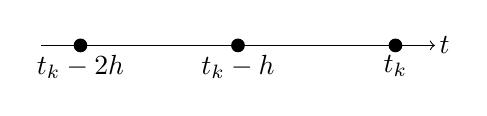
\begin{tikzpicture}[scale=2, domain=-0.5:2.5]
	\draw[->] (-.25,0) -- (2.25,0) node[pos=1.025] {$t$};
	\draw[fill=black] (0,0) circle [radius=0.04] node[below] {$t_k - 2h$};
	\draw[fill=black] (1,0) circle [radius=0.04] node[below] {$t_k - h$};
	\draw[fill=black] (2,0) circle [radius=0.04] node[below] {$t_k$};
	\end{tikzpicture}
	\end{center}

	For the Lagrange polynomials in the points $t_k$, $t_k -h$ resp. $t_k -2h$ we have
	\begin{gather*}
		L_0 (t) = \tfrac{t-(t_k-h)(t-t_k)}{2h^2}, \,
		L_1 (t) = \tfrac{(t-t_k)(t-t_kj-2h)}{h^2} \, \text{resp.} \,
		L_2 (t) =  \tfrac{(t-t_k+2h)(t-t_k+h)}{2h^2}.
	\end{gather*}

	As announced, we assume that the interpolation polynomial fulfilles the IVP in 
	the point $t_k$, i.e. there holds $f_k := f(t_k, y(t_k)) = y'(t_k) = \sum_{j=1} ^s 
		y_{k-j} L_{k-j} ' (t)$. The product rule and evaluation at $t=t_k$ yields

	\begin{gather*}
		L_0 '(t) = \tfrac{2t-2t_k+h}{2h^2} = \tfrac{1}{2h}, \,
		L_1 '(t) = -\tfrac{2t -2t_k + 2h}{h^2} = -\tfrac{2}{h}  \, \text{and} \,
		L_2 '(t) = \tfrac{2t-2t_k + 3h}{2h^2} = \tfrac{3}{2h}. 
	\end{gather*}

	Then, we obtain 
	\begin{gather*}
		f_k = \tfrac{1}{2h} y_{k-2} - \tfrac{2}{h}y_{k-1} + \tfrac{3}{2h} y_k.
	\end{gather*}
	Multiplication with $\tfrac{2}{3h}$ yields the scheme
	\begin{gather*}
		y_k - \tfrac{4}{3} y_{k-1} + 3y_{k-2} = \tfrac{2}{3h} f_k.
	\end{gather*}

%%% Local Variables: 
%%% mode: latex
%%% TeX-master: "notes"
%%% End: 

\bibliographystyle{alpha}
\bibliography{skript}
\printindex

%%% Local Variables: 
%%% mode: latex
%%% TeX-master: "notes"
%%% End: 



\printbibliography
\printindex


%%% Local Variables: 
%%% mode: latex
%%% TeX-master: "main"
%%% End: 
